\documentclass[a4paper,11pt,openany]{book} %draft faz aparecer uns quadrados pretos no fim de alguns math mode e imagens, então não esquenta se aparecer

\usepackage[portuguese]{babel}
\usepackage[utf8]{inputenc}
\usepackage{enumerate}
\usepackage[a4paper,includemp,includefoot, twoside=true, inner=1.25in, outer=0.75in]{geometry} 
\usepackage{marginnote}
\usepackage{multicol}
\usepackage{mathtools}
\usepackage{amssymb}
\usepackage{amsfonts}
\usepackage{amsthm}
\usepackage{pifont}
\usepackage[T1]{fontenc}
\usepackage[scaled]{berasans}
\usepackage{gensymb}
\usepackage[table, xcdraw]{xcolor}
\usepackage{tikz}
\usepackage{graphics}
\usepackage{graphicx}
\usepackage{pgfplots}
    \usetikzlibrary{intersections}
	\usetikzlibrary{patterns}
	\usetikzlibrary{calc}
    \usetikzlibrary{matrix}
    \usetikzlibrary{cd}
	\usepgfplotslibrary{fillbetween}
\usepackage[colorlinks=false]{hyperref}
\usepackage{blindtext}
\usepackage{float}
\usepackage{caption}
\usepackage{subcaption}
\usepackage[super, square]{natbib}
\usepackage{comment}
\usepackage{polynom}
\usepackage{framed}
\usepackage{minitoc}

\newtheorem{teo}{Teorema}[chapter]
\newtheorem{post}{Postulado}[part]
\newtheorem*{lema}{Lema}
\theoremstyle{definition} \newtheorem*{df}{Definição}
\newtheorem*{prop}{Propriedade}

\newcounter{examplecounter}
\newenvironment{exemplo}
	{\begin{framed}\noindent \refstepcounter{examplecounter} {\textbf{Exemplo \arabic{examplecounter}.}} }
    {\end{framed}}

\setcounter{parttocdepth}{2} %default
\setlength{\ptcindent}{0pt} %default
\renewcommand{\ptcfont}{\normalsize\rm} %default
\renewcommand{\ptcCfont}{\normalsize\bf} %default
\renewcommand{\ptcSfont}{\normalsize\rm} %default

\renewcommand\beforeparttoc{}
\renewcommand\afterparttoc{}

\mtcsettitle{parttoc}{Sumário}

\newenvironment{note}{\par \vspace{10pt} \textsc{Versão Humana}\\ \begin{small}}{\\ \noindent\hrule \vspace{10pt} \end{small}}

%%%%%%      TRIGONOMETRICAS - as que precisam e as que não precisam também      %%%%%%
\providecommand{\sin}{} \renewcommand{\sin}{\hspace{2pt}\mathrm{sen}}
\providecommand{\cos}{} \renewcommand{\cos}{\hspace{2pt}\mathrm{cos}}
\providecommand{\tan}{} \renewcommand{\tan}{\hspace{2pt}\mathrm{tg}}
\providecommand{\sec}{} \renewcommand{\sec}{\hspace{2pt}\mathrm{sec}}
\providecommand{\csc}{} \renewcommand{\csc}{\hspace{2pt}\mathrm{cossec}}
\providecommand{\cot}{} \renewcommand{\cot}{\hspace{2pt}\mathrm{cotg}}

\bibliographystyle{docs/plainnapt}

\captionsetup[table]{skip=10pt}

\author{(Cristian, Eduarda, Gustav, Tomás, Vanessa) \and Cristian Brenner\\ cristianbobsin@gmail.com \and Eduarda Machado\\ eduardamachado00@gmail.com \and Gustav Beier\\ gustavbeier@gmail.com \and Tomás Branco\\ tomasdbranco@hotmail.com \and Vanessa Martins\\ vanessadsilvamartins@gmail.com}
\title{ \textsc{5-upla} }
\date{}

\begin{document}

\maketitle
\newpage \thispagestyle{empty} \null
\newpage
%\chapter*{Agradecimentos}
%Zé, Vandoir, Daniela, [...] ?
\chapter*{Prefácio}
%objetivos desta apostila, como fizemos ela,gostariamos de ressaltar que as notas dos autores NÃO SÃO FORMAIS - apenas apontamentos de alunos que passaram pelo mesmo que você.
	\doparttoc
	\dopartlof
	\dopartlot
\faketableofcontents
\fakelistoffigures
\fakelistoftables

\part{Álgebra}
	\parttoc
%\chapter{Teoria dos Conjuntos}

Conjunto é uma coleção de elementos, não importando a ordem ou quantidade de vezes em que estes se apresentam. Qualquer coisa é um elemento em potencial. Se um elemento $x$ faz parte de um conjunto $A$, é dito $x \in A$. Se ele não faz parte, $x \not \in A$.

\begin{df}
Um conjunto é dito \emph{subconjunto} de outro se todos os elementos do primeiro pertencerem ao segundo. \[A \subset B \Leftrightarrow (\forall x) (x\in A \rightarrow x \in B)\].
\end{df}
\vspace{-24pt}
\begin{df}
Dois conjuntos são ditos \emph{iguais} se todos os elementos de um pertencerem ao outro e vice-versa.\[A=B \Leftrightarrow (\forall x)(x \in A \leftrightarrow x \in B)\]
\end{df}
\begin{df}
O número de elementos de um conjunto é chamado de \emph{cardinalidade} e é denotado por $|A|$.
\end{df}
\section{Representação de Conjuntos\cite{ticj}}
Conjuntos são usualmente denotados por letras latinas maiúsculas, enquanto seus elementos são normalmente denotados por letras latinas minúsculas ou por letras minúsculas munidas de índices numéricos. 

\subsection*{Extensão}
A forma mais simples de representar os elementos de um conjunto entre chaves, listando-os.
\begin{exemplo}
\[A=\{a_1,a_2,a_3,..., a_n\}\]
\end{exemplo}

\subsection*{Compreensão}
Podemos representar um conjunto especificando os seus elementos através de uma proposição. \begin{exemplo}
\[A=\{a_i | 0<i \le n\}\]
\end{exemplo}

\subsection*{Diagrama de Euler-Venn}
Podemos representar conjuntos através dos diagramas de Euler-Venn. Conjuntos finitos podem ser proveitosamente representados, por um plano determinado por uma linha fechada não entrelaçada inscrita em um quadrado ou retângulo. Nesse diagrama, os elementos do conjunto são representados por pontos internos ao recinto e elementos que não pertencem ao conjunto são representados por pontos externos. \par 
Um dos benefícios de representar conjuntos por meio de diagramas de Euler-Venn é a fácil visualização de subconjuntos, intersecções e outras regiões definidas nos conjuntos.
\begin{comment}
\begin{figure}[H]
  \caption{Diagrama de Euler-Venn}
  \centering
  \includegraphics[width=0.5\textwidth]{images/venn}
\end{figure}
\end{comment}

\section{Conjuntos Conhecidos}
Ao longo da nossa vida de estudante, somo expostos de maneira progressiva a conjuntos numéricos que se tornam, depois de um tempo, conhecidos. De início, temos os naturais, que também são conhecidos como números de contagem. Depois, se expandem para os Inteiros, que é quando somos apresentados aos números negativos.%colocar footnote sobre controversias nesta definição%. 
Na sequência temos os racionais e suas dizimas e frações, juntamente somos apresentados aos Irracionais. Para juntar todos estes números, unimos os conjuntos $\mathbb{Q}$ e $\mathbb{I}$ e obtemos os reais. Entretanto, observe a imagem abaixo:\\
%colocar uma imagem errada de conjuntos%
Se os reais podem ser definidos como a união dos conjuntos $\mathbb{Q}$ e $\mathbb{I}$, o que tem no espaço hashurado?
Por fim, temos os Complexos, que podem ou não ser trabalhados na educação básica, mas saiba você, aluno da graduação de matemática, que eles existem.

\subsection{Conjuntos Numéricos}
\subsubsection{$\mathbb{N}$ - Números Naturais}
Os números naturais são aqueles utilizados para contagem e ordenação. De forma ampla, os números naturais são uma propriedade de um conjunto: o conjunto $\{1,\alpha,4,a\}$ apresenta a propriedade $4$, pois possui quatro elementos. \[\mathbb{N}=\{0,1,2,3,4,5,\dots \}\]

\subsubsection{$\mathbb{Z}$ - Números Inteiros}
O conjunto dos números inteiros é formado pelos números naturais e seus opostos aditivos, constituindo um grupo com a operação adição definida. \[\mathbb{Z}=\{\dots, -3, -2, -1, 0, 1, 2, 3, \dots\}\]

\subsubsection{$\mathbb{Q}$ - Números Racionais}
O conjunto dos números racionais é derivado do conjunto dos números inteiros. Os números racionais são formados por frações de inteiros, representando partes de um inteiro. O conjunto $\mathbb{Q}$ é definido por \[\mathbb{Q}=\left\lbrace \frac{a}{b} \: | \: a,b \in \mathbb{Z}, b \neq 0 \right\rbrace\]

\subsubsection{$\mathbb{I}$ - Números Irracionais}
Os números irracionais são aqueles que não podem ser escritos como uma fração de inteiros (aqueles que não são racionais). Estes são constantes com infinitas casas decimais não-periódicas e raízes. São estes os números reais algébricos e transcendentes.
\subsubsection{$\mathbb{R}$ - Números Reais}
O conjunto dos números reais é definido por \[\mathbb{R}=\mathbb{Q} \cup \mathbb{I}\] e pode ser interpretado como todos os valores reais, como medidas.

\subsubsection{$\mathbb{C}$ - Números Complexos}
O conjunto dos números complexos é gerado a partir das raízes de índice par de números negativos. Os números são formados de uma parte real e uma parte imaginária - composta pela unidade $i$. O conjunto é definido como \[\mathbb{C}=\{a+bi \ | \ a,b \in \mathbb{R}, i^2=-1\}\]

\subsection{Conjunto Vazio}
O conjunto vazio, representado por $\emptyset$, é o conjunto que não possui elementos. Portanto, \[(\forall x)(x \in \emptyset) \: \Rightarrow \: F\]

\subsection*{Outros Conjuntos}
\begin{df}
O conjunto de todos os subconjuntos de $A$ é chamado de \emph{conjunto das partes}, conjunto potência ou apenas partes de $A$. É denotado por $\mathcal{P}(A)$ ou $2^A$. \begin{exemplo}
\[A=\{1, 2, 3\}\]
\[\mathcal{P}(A)=\{\emptyset, \{1\}, \{2\}, \{3\}, \{1,2\}, \{1,3\}, \{2,3\}, \{1,2,3\}\}\]
\end{exemplo}
O conjunto é denotado por $2^{A}$ pois possui exatamente $2^{|A|}$ elementos.
\end{df}
\begin{df}
Uma família de subconjuntos $\{A_i \: | \: i \in I\}$ de um conjunto $A$ é dita uma \emph{partição} de A se as seguintes propriedades são cumpridas:
\begin{itemize}
	\item $A_i \neq \emptyset, \forall i \in I$
	\item $\bigcup\limits_{i \in I} A_i = A$
	\item $A_i \cap A_j \neq \emptyset \Rightarrow A_i =A_j$
\end{itemize}
\end{df}

\section{Operações}
%texto, se quiser.
\subsection*{União}
O união de dois conjuntos resulta em um conjunto que possui os elementos de ambos os conjuntos.
\[A \cup B = \{x \: | \: x\in A \vee x \in B\}\]
\begin{figure}[H]
  \caption{União}
  \centering
  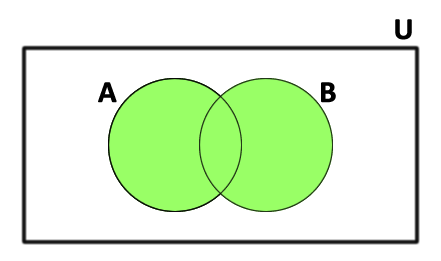
\includegraphics[width=0.5\textwidth]{algebra/imagens/uni}
\end{figure}

\subsection*{Intersecção}
A intersecção entre dois conjuntos é o subconjunto que possui os elementos que pertencem a ambos os conjuntos simultaneamente.
\[A \cap B = \{x \: | \: x\in A \wedge x \in B\}\]
\begin{figure}[H]
  \caption{Intersecção}
  \centering
  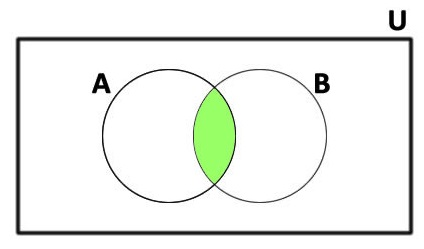
\includegraphics[width=0.5\textwidth]{algebra/imagens/intersect}
\end{figure}

\subsection*{Diferença}
A diferença entre $A$ e $B$ é o subconjunto que possui os elementos de $A$ que não são elementos de $B$.
\[A \smallsetminus B = \{x \: | \: x \in A \wedge x \not \in B\}\]
\begin{figure}[H]
  \caption{Diferença}
  \centering
  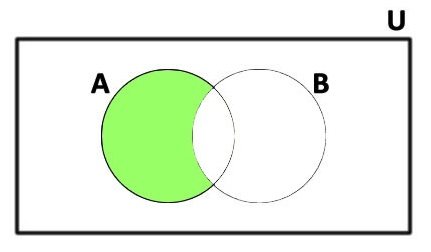
\includegraphics[width=0.5\textwidth]{algebra/imagens/diferen}
\end{figure}

\subsection*{Complementar}
O complementar de um conjunto $A$ é o conjunto de todos os elementos que não fazem parte de $A$.
\[A^{c}=\{x \: | \: x \not \in A\}\]
\begin{figure}[H]
  \caption{Complementar}
  \centering
  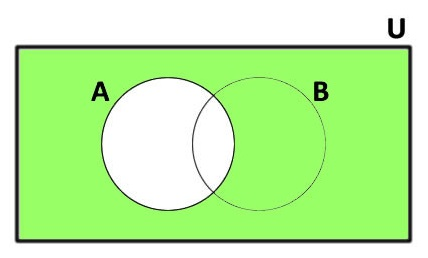
\includegraphics[width=0.5\textwidth]{algebra/imagens/comp}
\end{figure}

\subsection*{Diferença Simétrica}
A diferença simétrica $A \Delta B$ é o conjunto dos elementos que pertencem a apenas um dos conjuntos. Pode ser vista como a diferença entre a união e a intersecção $(A \cup B) - (A \cap B)$ ou como a união das diferenças $(A-B) \cup (B-A)$.
\[A \Delta B= \{x \: | \: x \in A \cup B \wedge x \not \in A \cap B\}\]
\begin{figure}[H]
  \caption{Diferença Simétrica}
  \centering
  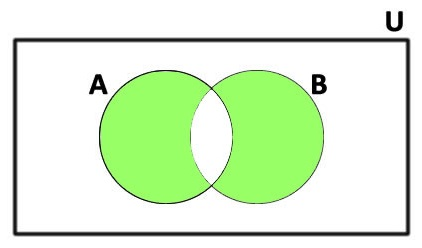
\includegraphics[width=0.5\textwidth]{algebra/imagens/difsim}
\end{figure}

\subsection*{Produto Cartesiano}
Originado apartir dos estudos de Descartes, que teve sua origem apartir da fundamentação da geometria analítica, o produto cartesiano (ou direto) é uma operação que relaciona  elementos de dois conjuntos em um elemento só.
\[A \times B = \{(x,y) \: | \: x \in A, y \in B\}\]
\chapter{Relações}
Uma relação é um subconjunto de um produto cartesiano. Pode ser definida por uma lei ou pares ordenados escolhidos manualmente. É importante, quando iniciar os estudos sobre relações, fazer uso das representações gráficas como recurso visual para compreender o que está sendo enunciado. Outra observação importante é consolidar o conceito de um conjunto contínuo e conjunto discreto, com estas duas noções bem estabelecidas, ter-se-a mais confiança nas afirmações e respostas sobre relações.

\section{Representação de Relações}
Relações são subconjuntos de produtos cartesianos. Quando lidamos com relações entre conjuntos numéricos, temos um conjunto de pontos do plano cartesiano. Essa relação pode ser contida em quaisquer subconjuntos dos números reais. \par 
Para representar os pontos que pertencem a relação, utilizamos linhas sólidas, delimitando extremidades de segmentos com pontos fechados e regiões com áreas pintadas. Para representar pontos que não pertencem a relação, utilizamos linhas tracejadas, pontos abertos e regiões não-pintadas.

\begin{exemplo}
A relação $R \subseteq \mathbb{Z} \times \mathbb{R}, xRy \Leftrightarrow x^2 \ge y$ pode ser representada como no plano cartesiano abaixo.
\begin{figure}[H] 
\centering
	\begin{tikzpicture}
		\begin{axis}[
		axis lines = middle,
        xtick = {-4,-3,...,4},
        ytick = {0,1,...,8},
		xmin = -4.5,
        xmax = 4.5,
		ymin = 0,
        ymax = 9, 
        xlabel = $x \in \mathbb{Z}$,
        ylabel = $y \in \mathbb{R}$]
        \addplot[
        domain = -5:5,
        samples = 100,
        loosely dashed
        ]{x^2};
        \addplot+[ycomb, mark=o, black] plot coordinates
{(-4,16) (-3,9) (-2,4) (-1,1) (0,0) (1,1) (2,4) (3,9) (4,16)};
		\end{axis}
	\end{tikzpicture}
    \caption[Exemplo de Relação]{$R=\{(x,y) \in \mathbb{Z} \times \mathbb{R} \mid y<x^2\}$}
\end{figure}
\end{exemplo}

\section{Operações entre Relações}
Relações são conjuntos de pares ordenados e, portanto, podemos utilizar as operações de conjuntos entre relações. Para facilitar a visualização, essas operações também são representadas no plano cartesiano.


\begin{exemplo}

Dadas as relações $R \subseteq \mathbb{R}^2, xRy \Leftrightarrow x^2+y^2 < 4$  e $S \subseteq \mathbb{R}^2, xSy \Leftrightarrow y \ge x+2$, temos:

\begin{center}
\begin{tikzpicture}
    \begin{axis}[
        unit vector ratio* = 1 1 1,
        axis lines = middle,
        xtick = {-2,2},
        ytick = {-2,2},
		xmin = -3,
        width = 0.8\textwidth,
        height = 0.6\textwidth,
        xmax = 3,
		ymin = -3,
        ymax = 3, 
        xlabel = $x$,
        ylabel = $y$
      ]  
      \addplot[samples=100, domain=-2:2, dashed, name path=A] {sqrt(-x^2+4)}; 
      \addplot[samples=100, domain=-2:2, dashed, name path=B] {-sqrt(-x^2+4)}; 
      \path[name path=xaxis] (\pgfkeysvalueof{/pgfplots/xmin}, -3) -- (\pgfkeysvalueof{/pgfplots/xmax},3);
      \addplot[gray, color=lime!60!white] fill between[of=A and B, soft clip={domain=-3:3}];
  \end{axis}
  \end{tikzpicture}%
\quad \begin{tikzpicture}
    \begin{axis}[
        unit vector ratio* = 1 1 1,
        axis lines = middle,
        xtick = {-2},
        ytick = {2},
		xmin = -3,
        xmax = 3,
		ymin = -3,
        ymax = 3, 
        xlabel = $x$,
        ylabel = $y$,
        width = 0.8\textwidth,
        height = 0.6\textwidth,
      ]  
      \addplot[samples=100, domain=-3:2, name path=A] {x+2}; 
      \addplot[samples=100, domain=-3:1, color=olive!60!white,  name path=B] {3}; 
      \path[name path=xaxis] (\pgfkeysvalueof{/pgfplots/xmin}, -3) -- (\pgfkeysvalueof{/pgfplots/xmax},3);
      \addplot[gray, color=olive!60!white] fill between[of=A and B, soft clip={domain=-3:3}];
  \end{axis}
  \end{tikzpicture} \\
  \end{center}
  E abaixo podemos visualizar algumas operações entre as relações.
  \begin{center}
  \begin{tikzpicture}
    \begin{axis}[
        unit vector ratio* = 1 1 1,
        axis lines = middle,
        xtick = {-2,2},
        ytick = {-2,2},
		xmin = -3,
        xmax = 3,
		ymin = -3,
        ymax = 3, 
        xlabel = $x$,
        ylabel = $y$,
        width = 0.8\textwidth,
        height = 0.6\textwidth,
      ]  
     \addplot[samples=100, domain=-2:2, color=olive!60!white, name path=A] {sqrt(-x^2+4)}; 
      \addplot[samples=100, domain=-2:2, color=lime, name path=B] {-sqrt(-x^2+4)}; 
       \addplot[samples=100, domain=-3:3,  name path=C] {x+2};
        \addplot[samples=100, domain=-3:1, color=white, name path=D] {3};
        \addplot[samples=100, domain=0:3, dashed, name path=E] {sqrt(-x^2+4)}; 
      \addplot[samples=100, domain=-3:3, dashed, name path=F] {-sqrt(-x^2+4)}; 
      \path[name path=xaxis] (\pgfkeysvalueof{/pgfplots/xmin}, -3) -- (\pgfkeysvalueof{/pgfplots/xmax},3);
      \addplot[gray, color=lime!60!white] fill between[of=A and B, soft clip={domain=-3:3}];
   \addplot[gray, color=olive!60!white] fill between[of=C and D, soft clip={domain=-3:3}];
  \end{axis}
  \end{tikzpicture}%
  \begin{tikzpicture}
    \begin{axis}[
        unit vector ratio* = 1 1 1,
		width = 0.8\textwidth,
        height = 0.6\textwidth,
        axis lines = middle,
        xtick = {-2,2},
        ytick = {-2,2},
		xmin = -3,
        xmax = 3,
		ymin = -3,
        ymax = 3, 
        xlabel = $x$,
        ylabel = $y$
      ]  
      \addplot[samples=100, domain=-2:0, dashed, name path=A] {sqrt(-x^2+4)}; 
       \addplot[samples=100, domain=-3:4, thin, dashed, name path=E] {x+2};
       \addplot[samples=100, domain=-2:0, name path=B] {x+2}; 
         \addplot[samples=100, domain=0:2, dashed, name path=C] {sqrt(-x^2+4)}; 
      \addplot[samples=100, domain=-2:2, dashed, name path=D] {-sqrt(-x^2+4)}; 
      \path[name path=xaxis] (\pgfkeysvalueof{/pgfplots/xmin}, -3) -- (\pgfkeysvalueof{/pgfplots/xmax},3);
      \addplot[gray, color=lime!60!white] fill between[of=A and B, soft clip={domain=-3:3}];
  \end{axis}
  \end{tikzpicture} \\
   \begin{tikzpicture}
    \begin{axis}[
        unit vector ratio* = 1 1 1,
        axis lines = middle,
        width = 0.8\textwidth,
        height = 0.6\textwidth,
        xtick = {-2,2},
        ytick = {-2,2},
		xmin = -3,
        xmax = 3,
		ymin = -3,
        ymax = 3, 
        xlabel = $x$,
        ylabel = $y$
      ]  
      \addplot[samples=100, domain= -5:0, white, name path=A] {sqrt(-x^2+4)};
       \addplot[samples=100, domain=-2:0, dashed, name path=B] {x+2}; 
         \addplot[samples=100, domain=-5:5, dashed, name path=C] {sqrt(-x^2+4)}; 
      \addplot[samples=100, domain=-5:5, dashed, name path=D] {-sqrt(-x^2+4)}; 
      \path[name path=xaxis] (\pgfkeysvalueof{/pgfplots/xmin}, -3) -- (\pgfkeysvalueof{/pgfplots/xmax},3);
      \addplot[gray, color=lime!60!white] fill between[of=C and D, soft clip={domain=-3:3}];
       \addplot[gray, color=white] fill between[of=B and A, soft clip={domain=-3:3}];
  \end{axis}
  \end{tikzpicture}%
  \begin{tikzpicture}
    \begin{axis}[
        unit vector ratio* = 1 1 1,
        axis lines = middle,
        xtick = {-2,2},
        ytick = {-2,2},
        width = 0.8\textwidth,
        height = 0.6\textwidth,
		xmin = -3,
        xmax = 3,
		ymin = -3,
        ymax = 3, 
        xlabel = $x$,
        ylabel = $y$
      ]  
      \addplot[samples=100, domain=-2:0,  name path=A] {sqrt(-x^2+4)};
      \addplot[samples=100, domain=-5:5, dashed, name path=A] {sqrt(-x^2+4)}; 
      \addplot[samples=100, domain=-5:5, dashed, name path=B] {-sqrt(-x^2+4)}; 
      \addplot[samples=100, domain=-5:5, dashed, name path=C] {x+2}; 
      \addplot[samples=100, domain=-5:-2, name path=C_1] {x+2}; 
      \addplot[samples=100, domain=0:5, name path=C_2] {x+2}; 
      \addplot[samples=100, domain=-5:1, color=lime!60!white,  name path=D] {3}; 
      \path[name path=xaxis] (\pgfkeysvalueof{/pgfplots/xmin}, -3) -- (\pgfkeysvalueof{/pgfplots/xmax},3);
      \addplot[gray, color=olive!60!white] fill between[of=C and D, soft clip={domain=-3:3}];
   \addplot[gray, white] fill between[of=A and B, soft clip={domain=-3:3}];
  \end{axis}
  \end{tikzpicture}
  \end{center}
É importante ressaltar o cuidado a ser tomado com as extremidades das relações, onde as linhas são tracejadas ou preenchidas.
\end{exemplo}


\section{Propriedades das Relações}
\begin{itemize}
	\item \textbf{Reflexiva}: uma relação é dita reflexiva quando todo elemento $x$ se relaciona consigo mesmo, ou seja, existe o par $(x,x)$ para qualquer $x$.
	\item \textbf{Irreflexiva}: uma relação é dita irreflexiva se nenhum $x$ se relaciona consigo mesmo, ou seja, não existe o par $(x,x)$ para qualquer $x$.
	\item \textbf{Simétrica}: uma relação é dita simétrica se para todo par $(x,y)$ da relação, existe o par $(y,x)$.
	\item \textbf{Anti-simétrica}: uma relação é dita anti-simétrica se para todo par $(x,y)$ da relação, o par $(y,x)$ existe apenas se $x=y$.
\item \textbf{Assimétrica}: uma relação é dita assimétrica se para todo par $(x,y)$ da relação, não existe o par $(y,x)$.
	\item \textbf{Transitividade}: uma relação é dita transitiva se para quaisquer pares $(x,y)$ e $(y,z)$ da relação existe o par $(x,z)$.
\end{itemize}

\section{Relações de Equivalência}
Relações são ditas de \emph{equivalência} quando apresentam a simetria, a transitividade e a reflexividade. Estas relações definem subconjuntos nos quais os elementos se relacionam apenas entre si. Esses subconjuntos, chamados classes de equivalência, geram uma partição do conjunto inicial.
\begin{exemplo}
A relação $R \subseteq \mathbb{Q} \times \mathbb{Q}$: \[R = \left\lbrace(\frac{a}{b},\frac{c}{d}) \in \mathbb{Q} \times \mathbb{Q} \: | \: ad=bc\right\rbrace\] gera uma partição em $\mathbb{Q}$, onde cada elemento da partição é uma classe de frações equivalentes.
\end{exemplo}

\section{Relações de Ordem}
Um conjunto de pessoas, assim como um conjunto qualquer, podem apresentar uma relação de ordem. Desta forma, não significa necessariamente que existe uma maior importância entre elementos, mas sim uma ordenação. É possível - por meio da observação, por exemplo - que exista uma certa ordem em um processo, um planejamento, uma empresa, ou entre números.\par 
Como estamos em um material matemático, uma relação de ordem em um conjunto, significa dizer que quando relacionando dois a dois, um sempre será maior ou igual ao outro.

\subsection{Ordem Parcial}
Uma relação de ordem é dita \emph{parcial} se existem elementos que não se relacionam (em qualquer ordem).
\[R \subset A \times A , \ \left(\exists x,y \in A \right)\left( (x,y), (y,x) \not \in R \right)\]

\paragraph*{Ampla}
Uma relação de ordem parcial ampla é aquela em que $x R x$, como na relação ``... maior ou igual a ...'', onde todo número é igual a ele mesmo e, portanto, é maior ou igual.
\begin{itemize}
\item \textbf{Transitividade}:``se $x\ge y$ e $y\ge z$, então $x\ge z$''
\item \textbf{Antissimetria}: ``se $x\ge y$ e $y \ge x$, então $y =x$''
\item \textbf{Reflexividade}: ``$x \ge x$''
\end{itemize}

\paragraph*{Estrita}
Uma relação de ordem parcial estrita é aquela em que $(x,x) \not \in R$, como na relação ``... maior do que ...'', onde nenhum número é maior do que ele mesmo.
Assim, pode ser definida a partir de três propriedades:
\begin{itemize}
\item \textbf{Transitividade}:``se $x>y$ e $y>z$, então $x>z$''
\item \textbf{Assimetria}: ``se $x>y$, $y\not > x$''
\item \textbf{Irreflexividade}: ``$x \not > x$''
\end{itemize}

\subsection{Ordem Total}
Uma relação de ordem é chamada de \emph{ordem total} quando quaisquer dois elementos se relacionam. 
\paragraph*{Ampla}
A relação é dita ampla quando existem apenas duas opções, como na relação ``... maior ou igual a ...''.
\[\forall x,y \in A \left( x \le y \vee y \le x \right)\]
Este tipo de relação apresenta a chamada \emph{dicotomia}, onde todos os elementos se encaixam em uma das duas opções.

\paragraph*{Estrita}
A relação é dita estrita quando existem duas opções, ou seja, quando $x=x \Rightarrow (x,x) \not \in R$ então temos três casos: 
\[\forall x,y \in A \left( x=y \vee x < y \vee y < x \right)\]
Este tipo de relação apresenta a chamada \emph{tricotomia}, onde todos os elementos se encaixam em uma das três opções.

\subsection{Ordem Densa}
Uma relação de ordem em um conjunto é dita \emph{densa} se para todos elementos $x,y \in A$ existe algum elemento $z$ entre $x$ e $y$.
\[\forall x,y \in A \left( x<y \Rightarrow \exists z \in A \left(x<z<y\right) \right)\] \par 
O conjunto dos números reais é o principal exemplo de conjunto com uma relação de ordem densa, pois para quaisquer elementos $x,y \in \mathbb{R}$ tais que $x < y$, existe $\frac{x+y}{2} \in \mathbb{R}$ tal que $x < \frac{x+y}{2} < y$.

\begin{figure}[H]
\centering
	\begin{subfigure}[b]{0.3\textwidth}
	\centering
		\begin{tikzpicture}
			\node (a) at (0,0) {$1$};
			\node (b) at (-1,1) {$2$};
			\node (c) at (1,1) {$3$};
			\node (d) at (0,2) {$6$};
			\node (e) at (1,2) {$9$};
			\node (f) at (-1,2) {$4$};
			\node (g) at (1,3) {$18$};
			\node (h) at (-1,3) {$24$};
			\node (i) at (0,4) {$72$};
			\draw (a) -- (b) -- (d) -- (g) -- (e) -- (c) -- (a);
			\draw (a) -- (b) -- (f) -- (h) -- (d) -- (c);
			\draw (h) -- (i) -- (g);
		\end{tikzpicture}
	\caption{Ordem Parcial}
	\end{subfigure}
	\quad
	\begin{subfigure}[b]{0.3\textwidth}
	\centering
		\begin{tikzpicture}
			\node (a) at (0,0) {$0$};
			\node (b) at (0,1) {$1$};
			\node (c) at (0,2) {$2$};
			\node (d) at (0,3) {$3$};
			\node (e) at (0,4) {$\vdots$};
			\draw (a) -- (b) -- (c) -- (d) -- (e);
		\end{tikzpicture}
	\caption{Ordem Total}
	\end{subfigure}
	\quad 
	\begin{subfigure}[b]{0.3\textwidth}
	\centering
		\begin{tikzpicture}
			\node (a) at (0,0) {$0$};
			\node (b) at (0,1) {$\vdots$};
			\node (c) at (0,2) {$1$};
			\node (d) at (0,3) {$\vdots$};
			\node (e) at (0,4) {$2$};
			\draw (a) -- (b) -- (c) -- (d) -- (e);
		\end{tikzpicture}
	\caption{Ordem Densa}
	\end{subfigure}
\caption{Diagramas de Hasse}
\end{figure}

\section{Funções}
\begin{df}
Sejam A e B dois conjuntos. Chamamos de \emph{função de $A$ em $B$} a uma relação que cada elemento de $A$ associa um único elemento de $B$, e denotamos simbolicamente por \begin{align*}
f: \ &A \rightarrow B \\
     &a \rightsquigarrow f(a)
\end{align*}
onde cada $a \in A$ está associado um único $b=f(a) \in B$. Chamamos $A$ de \emph{domínio da função $f$} e $B$ de \emph{contradomínio da função $f$}.
\end{df}
Uma função é uma relação entre dois conjuntos que relaciona um elemento de um conjunto (domínio) com um único do outro (contradomínio). Por definição, todo elemento do domínio precisa se relacionar com exatamente um elemento do contradomínio. O elemento do contradomínio correspondente ou do domínio é chamado de ``imagem'' ($\textrm{Im} \: f$). É importante saber que enquanto todo elemento do domínio precisa ter uma imagem, nem todo elemento do contradomínio precisa ter um correspondente do domínio.\par 

\begin{exemplo}
Seja a função $f$:\[f=\{(0,1),(2,5),(3,4),(5,8)\}\]
%imagem de funcao de um elipsoide pro outro
\end{exemplo}

Se $X \subset A$ e $f: A \rightarrow B$ denotamos por $f(X)$ ao conjunto $f(X)=\{f(x) : x \in X\} \subset B$ o qual chamamos de \textit{imagem de X pela f}. \par 
Se $f: A \rightarrow B$ é uma função e $y \in B$, denotamos por $f^{-1}(y)$ ao conjunto $f^{-1}(y)=\{x \in A : f(x)=y \}$ o qual chamamos de \emph{imagem inversa de $y$ pela $f$}. Se $y \not \in Im\:f$, $f^{-1}(y)= \emptyset$. \par 
Se $Y \subset B$ denotamos por $f^{-1}(Y)$ ao conjunto $f^{-1}(Y)=\{x\in A : f(x)=Y\}$ e chamamos tal conjunto de \emph{imagem inversa de $Y \subset B$ pela f}.

\subsection{Conjuntos}
\paragraph*{Domínio}
O \emph{domínio} de uma função, denotada como conjunto de partida, é o conjunto que contem todos os elementos de partida.
\paragraph*{Contradomínio}
O \emph{contradomínio} de uma função é o conjunto de chegada. O elemento parte do domínio e é associado a um do contradomínio.
\paragraph*{Imagem}
A \emph{imagem} de uma função é um conjunto contido no contradomínio cujos elementos são todos os elementos do contradomínio que são associados a um do domínio.\\
\begin{exemplo}
\begin{align*}
f: \ &\mathbb{N} \rightarrow \mathbb{R} \\
&x \rightsquigarrow x^2
\end{align*}
\end{exemplo}
Na nossa função f, nós temos como domínio $\mathbb{N}$ (conjunto de partida) e contradomínio $\mathbb{R}$ (conjunto de chegada). Nesse exemplo, podemos pegar um $x \in \mathbb{N}$, como 3, e seu elemento associado no contradomínio é o 9. O nosso conjunto $\textrm{Im} \, f$, portanto, é $\{0,1,4,9,16,25,\ldots\}$, que está contido em $\mathbb{R}$.

\subsection{Propriedades}
\paragraph{Injeção} Uma função é dita injetora quando: $\forall x,x'\in X, f(x)=f(x') \Rightarrow x=x'$. Ou seja, se dois elementos do domínio tem a mesma imagem, eles tem que ser o mesmo elemento. Isso nos diz que o conjunto $\textrm{Im} \,f$ tem o mesmo numero de elementos que nosso domínio.\\
\begin{exemplo}Seja a função $f$ definida por $f(x)=x^3$.\\
Vamos supor um x,x' tal que f(x)=f(x'). Para provarmos que a função é injetora, temos que provar que x=x'. Portanto:
\begin{align*}
&f(x)=f(x') &=\\
&(x)^3=(x')^3 &=\\
&\sqrt[3]{x^3}=\sqrt[3]{(x')^3}&=\\
&x=(x')
\end{align*}
\end{exemplo}

\paragraph{Sobrejeção} Uma função é sobrejetora quando $\forall y \in Y, \exists x \in X$ tal que $ y=f(x)$. Isso nos diz que todo y no contradomínio está contido na imagem, ou seja, $\textrm{Im} \, f$ e o contradomínio são iguais.\\
\begin{exemplo} Seja a função $f$ definida por $f(x)= x^3$. \par 
Queremos provar que todo y tem um x. Portanto:\\
\begin{align*}
&y=x^3 &=\\
&\sqrt[3]{y}=x
\end{align*}
Assim, temos que:
\begin{align*}
&f(\sqrt[3]{y}) &=\\
&(\sqrt[3]{y})^3 &= \\
&y
\end{align*}
\end{exemplo}

\paragraph{Bijeção} Uma função é bijetora quando ela satisfaz as condições de injeção e sobrejeção, ou seja, ela é sobrejetora e injetora. Como nos provamos nos últimos 2 seções que $f(x)=x^3$ é tanto injetora quanto sobrejetora, ela é uma função bijetora.\\
\begin{exemplo} Dada a função $f(x)= x+4$. 

%tabelinha de elipsoides que tem aqui: https://en.wikipedia.org/wiki/Bijection,_injection_and_surjection dai
\end{exemplo}

\subsection{Composição de Funções}
Se tivermos duas funções $f: A \rightarrow B$ e $g: B \rightarrow C$, uma função composta é denotada por: $f \circ g: A \rightarrow C$. $(f \circ g)(x)$ pode ser escrita em extenso como $f(g(x))$.\\
\begin{exemplo}
Se tivermos $f(x)=x+1$ e $g(x)=x^2$.\par 
$(f \circ g)(x)$ seria definida por:
\begin{align*}
&f(g(x)) &= \\
&f(x^2) &=\\
&x^2+1
\end{align*}
Enquanto $(g \circ f)(x)$ seria definida por:
\begin{align*}
&g(f(x)) &= \\
&g(x+1) &=\\
&(x+1)^2 &=\\
&x^2+2x+1
\end{align*}
\end{exemplo}
Com esse exemplo,podemos ver que a composição de funções não é comutativa.
%Elipsoides para mostrar comp. de funcoes. Aquela que tem 3 ovais e retas do 1 pro 2 pro 3. issae

\paragraph{Função Identidade} A função identidade, denominada por $\textrm{id}_x$, é uma função tal que $f \circ \textrm{id}_x=f$ e $\textrm{id}_x \circ f = f$. Essa função é $f(x)=x$.

\subsection{Função Inversa}
Uma função é \emph{inversível} se e somente se ela é bijetora. Ela leva um elemento do contradomínio para o domínio, e tem a propriedade $f^{-1}(f(x))=x$.
\begin{proof}
Suponhamos $f$ não-bijetora. Assim, $f$ não é injetora ou $f$ não é sobrejetora.\par 
Se $f$ não é injetora, existe $y \in CD f$ tal que $f^{-1}(y)={a,b} \subset D f$. Assim, existe $y \in D f^{-1}$ que possui duas imagens distintas e, portanto, $f^{-1}$ não é função.\par 
Se $f$ não é injetora, existe $y \in CD f$ tal que $f^{-1}(y)=\emptyset$. Assim, $f^{-1}$ possui um elemento de seu domínio que não possui imagem e, portanto, não é função.\par 
Logo, uma função é inversível se e somente se é bijetora.
\end{proof}

\section{Operações}
\begin{df}
Chamamos de \emph{operação (binária)} em um conjunto não vazio $A$ uma função
\begin{align*}
\mathcal{O}: A \times A &\rightarrow A \\
(a,b) &\rightsquigarrow \mathcal{O}(a,b)=a\mathcal{O}b
\end{align*}
A operação $\mathcal{O}$ é dita \emph{associativa} se $\forall a,b,c \in A$, tem-se $(a\mathcal{O}b)\mathcal{O}c=a\mathcal{O}(b\mathcal{O}c)$, e diz-se que é \emph{comutativa} se $\forall a,b \in A$, $a\mathcal{O}b=b\mathcal{O}a$.
\end{df}

%\chapter{Aritmética}
Para iniciarmos o estudo da Aritmética, precisamos definir o conjunto dos números naturais e o conjunto dos números inteiros. Assim, tomaremos a construção dos números naturais a partir do axiomas de Peano. \par 
Peano considera três entes primitivos: \emph{número natural}, \emph{zero}, e \emph{sucessor}. Iremos denotar \emph{zero} por $0$ e o sucessor de $n$ por $\sigma(n)$ Os axiomas apresentados são os seguintes: \begin{enumerate}[I.]
\item $0$ é um número natural;
\item $0$ não é sucessor de nenhum número natural;
\item Todo número natural $n$ tem um sucessor $\sigma(n)$;
\item Se $\sigma(m)=\sigma(n)$, então $m=n$.
\end{enumerate}
Tomemos agora um conjunto $\mathbb{N}$ de números naturais tal que $0\in \mathbb{N}$ e $\forall x \in \mathbb{N}, \sigma(x) \in \mathbb{N}$. Portanto, temos:
\begin{align*}
0 \in \mathbb{N} &\Rightarrow \sigma(0)=1 \in \mathbb{N} \\
1 \in \mathbb{N} &\Rightarrow \sigma(1)=2 \in \mathbb{N} \\
2 \in \mathbb{N} &\Rightarrow \sigma(2)=3 \in \mathbb{N} \\
&\vdots 
\end{align*}
Assim, $\mathbb{N}$ é o conjunto de números naturais que conhecemos. \par
Para definir a soma, usamos a função $\sigma: \mathbb{N} \rightarrow \mathbb{N}$ e definimos a função \[+ : \mathbb{N}\times\mathbb{N} \rightarrow \mathbb{N}\] em que $m+0=m$ e $m+\sigma(n)=\sigma(m+n)$.\par 
Podemos interpretar a soma como a contagem de ``sucessões'' que devemos tomar de $0$ a $m$ e a $n$, e $m+n$ seria equivalente a todas essas sucessões.

\section{Operações}
Já definimos uma operação nos Naturais, a \emph{adição}. Agora, iremos definir a \emph{multiplicação}:
\begin{align*}
\cdot: \mathbb{N}\times\mathbb{N} &\rightarrow \mathbb{N} \\
(a,b) &\mapsto ab=\begin{cases}
a\cdot 0 = 0 \\
a\cdot (b+1)=a \cdot b + a
\end{cases}
\end{align*} 
A partir de um certo número de propriedades (que podem ser demonstradas a partir dos axiomas de Peano e das definições acima), iremos construir as demais propriedades. São estas:
\begin{enumerate}[1)]
\item A adição e a multiplicação são \emph{bem definidas}: \[\forall a,b,a',b' \in \mathbb{N}, a=a',b=b' \Rightarrow a+b=a'+b'\textrm{ e }ab=a'b'\]
\item A adição e a multiplicação são \emph{comutativas}:\[\forall a,b \in \mathbb{N}, a+b=b+a \textrm{ e }ab=ba\]
\item A adição e a multiplicação são \emph{associativas}: \[\forall a,b,c \in \mathbb{N}, a+(b+c)=(a+b)=c \textrm{ e } a(bc)=(ab)c\]
\item A adição e a multiplicação possuem \emph{elementos neutros}: \[ \forall a \in \mathbb{N}, a+0=a \textrm{ e } a\cdot 1 =a\]
\item A multiplicação é \emph{distributiva }em relação à adição:\[\forall a,b,c \in \mathbb{N}, a(b+c)=ab+ac\]
\item \emph{Integridade}:
\[\forall a,b, \in \mathbb{N}, a\cdot b=0 \Rightarrow a=0 \textrm{ ou }b=0\]
\item \emph{Tricotomia}: Dados $a,b \in \mathbb{N}$, uma, e apenas uma, das seguintes possibilidades é verificada:
\[{a=b} \qquad  {\exists c \in \mathbb{N}^*, b=a+c} \qquad {\exists c \in \mathbb{N}^*, a=b+c}\]
Diremos que se $\exists c \in \mathbb{N}^*$ tal que $a=b+c$, então $a>b$. Assim, a tricotomia nos diz que, dados $a,b \in \mathbb{N}$ uma, e apenas uma, das seguintes condições é verificada:
\[{a=b} \qquad  {a>b} \qquad {a<b}\]
\end{enumerate}
A partir destas definições, podemos desenvolver as demais, todas estas conhecidas intuitivamente. Estas irão embasar nosso estudo de números inteiros mais adiante.

\begin{prop}
$\forall a \in \mathbb{N}^*,0<a$
\begin{proof}
Para qualquer $a \in \mathbb{N}^*$ temos que $0+a=a$. Sendo $a \in \mathbb{N}^*$, então $0<a$.
\end{proof}\end{prop}

\begin{prop}
$a+b=0 \Rightarrow a=b=0$
\begin{proof}
Suponhamos $a,b\in \mathbb{N}^*$. Assim, temos que $a<0$, o que é um absurdo. Portanto, $a=0$. Analogamente, provamos $b=0$. Portanto, se $a+b=0$, $a=b=0$.
\end{proof}\end{prop}

\begin{prop}
$\forall a \in \mathbb{N}, a\cdot 0 = 0$
\begin{proof}
\[a\cdot 0 = a \cdot (0+0) = a\cdot 0 + a\cdot 0\]
Se $a\cdot 0 = a\cdot 0 + a\cdot 0$, então $a\cdot 0 = 0$.
\end{proof}\end{prop}

\begin{prop}
A relação \emph{menor do que} é transitiva:
\[\forall a,b,c \in \mathbb{N}, a<b \textrm{ e }b<c \Rightarrow a<c\]
\begin{proof}
Se $a<b$ e $b<c$, então $\exists f ,g \in \mathbb{N}^*$ tais que $a+f=b$ e $b+g=c$. Portanto, $(a+f)+g=c$. Como $(f+g) \in \mathbb{N}^*$, então $a<c$.
\end{proof}\end{prop}
\begin{exemplo}
\begin{align*}
2<5 \textrm{ e } 5<6 &\Rightarrow 2<6 \\
4<9 \textrm{ e } 9<10 &\Rightarrow 4<10 \\
0<\alpha \textrm{ e } \alpha<\alpha+1 &\Rightarrow 0<\alpha+1
\end{align*}
\end{exemplo}

\begin{prop}
A adição é compatível e cancelativa com respeito à relação \emph{menor do que}:
\[\forall a,b,c \in \mathbb{N}, a<b \Leftrightarrow a+c<b+c\]
\begin{proof}
Se $a<b$, então existe $d\in \mathbb{N}^*$ tal que $a+d=b$. Assim, temos que $(a+d)+c=b+c$, ou seja, $(a+c)+d=(b+c)$. Como $d\in \mathbb{N}^*$, então $a+c<b+c$.\\ Suponhamos agora que $a+c<b+c$. Assim, temos três possibilidades:
\begin{enumerate}[(i)]
\item $a=b$. Se $a=b$, então $a+c=b+c$, o que é um absurdo.
\item $b<a$. Se $b<a$, então $b+c<a+c$, o que é um absurdo.
\item $a<b$. Esta é a única alternativa válida.
\end{enumerate}\end{proof}\end{prop}

\begin{prop}
A multiplicação é compatível e cancelativa em respeito à relação \emph{menor do que}:
\[\forall a,b \in \mathbb{N}, \forall c \in \mathbb{N}^*, a<b \Leftrightarrow a\cdot c < b \cdot c\]
\begin{proof}
Se $a<b$, então existe $d \in \mathbb{N}^*$ tal que $a+d=b$. Portanto, sendo $c \in \mathbb{N}^*$, temos que $c\cdot(a+d)=c\cdot b$, ou seja, $c\cdot a + c\cdot d = c\cdot b$. Como $c,d \in \mathbb{N}^*$, temos que $(c\cdot d) \in \mathbb{N}^*$ e, portanto, $c\cdot a < c\cdot b$.\\ Suponhamos agora que $a\cdot c<b\cdot c$. Assim, temos três possibilidades:
\begin{enumerate}[(i)]
\item $a=b$. Se $a=b$, então $a\cdot c=b\cdot c$, o que é um absurdo.
\item $b<a$. Se $b<a$, então $b\cdot c<a\cdot c$, o que é um absurdo.
\item $a<b$. Esta é a única alternativa válida.
\end{enumerate}\end{proof}\end{prop}

\begin{prop}
A adição é compatível e cancelativa com respeito à igualdade.
\[\forall a,b,c \in \mathbb{N}, a=b \Leftrightarrow a+c=b+c \]
\begin{proof}
A primeira implicação é direta, pois a adição é bem definida nos naturais. \\ Suponhamos agora que $a+c=b+c$. Assim, temos três possibilidades:
\begin{enumerate}[(i)]
\item $a<b$. Se $a<b$, então $a+c<b+c$, o que é um absurdo.
\item $b<a$. Se $b<a$, então $b+c<a+c$, o que é um absurdo.
\item $a=b$. Esta é a única alternativa válida.
\end{enumerate}\end{proof}\end{prop}

\begin{prop}
A multiplicação é compatível e cancelativa com respeito à igualdade.
\[\forall a,b \in \mathbb{N},\forall c \in \mathbb{N}^*, a=b \Leftrightarrow a\cdot c=b\cdot c \]
\begin{proof}
A primeira implicação é direta, pois a multiplicação é bem definida nos naturais. \\ Suponhamos agora que $a\cdot c=b\cdot c$. Assim, temos três possibilidades:
\begin{enumerate}[(i)]
\item $a<b$. Se $a<b$, então $a\cdot c<b\cdot c$, o que é um absurdo.
\item $b<a$. Se $b<a$, então $b\cdot c<a\cdot c$, o que é um absurdo.
\item $a=b$. Esta é a única alternativa válida.
\end{enumerate}
\end{proof}
\end{prop}

Para definirmos a subtração nos números naturais, temos que impor certas restrições:
\begin{df}
Dados dois números $a,b \in \mathbb{N}$ tais que $a\ge b$, sabemos que existe um número natural $c$ tal que $a=b+c$. Assim, denotaremos este número natural por $a-b=c$.
\begin{align*}
- : \mathbb{N}\times\mathbb{N}&\rightarrow\mathbb{N}\\
(a,b)&\mapsto a-b=c\Leftrightarrow a=b+c
\end{align*} \end{df}
\begin{exemplo}
\begin{align*}
3\ge 1 \textrm{ pois }\exists\: 2 \in\mathbb{N}\textrm{ tal que }& 3=2+1 \Rightarrow 3-1=2\\
8\ge 5 \textrm{ pois }\exists\: 3 \in\mathbb{N}\textrm{ tal que }& 8=5+3 \Rightarrow 8-5=3\\
0\ge 0 \textrm{ pois }\exists\: 0 \in\mathbb{N}\textrm{ tal que }& 0=0+0 \Rightarrow 0-0=0
\end{align*}
\end{exemplo}
Para ampliarmos o conjunto $\mathbb{N}$ dos números naturais, iremos criar o conjunto $\mathbb{Z}$ dos números inteiros. \par 

\section{Números Inteiros}
Consideremos o conjunto $\mathbb{N}$ dos números naturais e seja $E = \mathbb{N} \times \mathbb{N}$ o produto cartesiano de $\mathbb{N}$ por si mesmo. Já sabemos das propriedades definidas sobre $\mathbb{N}$, em relação a adição e a multiplicação. São estas:
\begin{align*}
(a+b)+c&=a+(b+c)& (ab)c&=a(bc)\\
a+b&=b+a& ab&=ba\\
a+0&=a& a\cdot 1&=a
\end{align*}
Além destas, temos:
\begin{align*}
a+c=b+c &\Rightarrow a=b\\
a(b+c)&=ab+ac
\end{align*}
Definiremos uma relação $\sim$ sobre $E$:
\[(a,b),(c,d) \in E, (a,b)\sim (c,d) \Leftrightarrow (a+d)=(b+c)\]
A relação $\sim$ é uma relação de equivalência, ou seja, é simétrica, reflexiva e transitiva.
\begin{proof}
Sejam $(a,b),(c,d),(e,f) \in E$. Assim, temos:
\[a+b=b+a \Rightarrow (a,b)\sim (a,b)\]
Suponhamos que $(a,b) \sim (c,d)$. Assim, $a+d=b+c$. Portanto, $d+a=c+b$, ou então $c+b=d+a$. Portanto, $(c,d)\sim (a,b)$. \\
Suponhamos $(a,b) \sim (c,d)$ e $(c,d) \sim (e,f)$. Portanto, $a+d=b+c$ e $c+f=d+e$. Consideremos, então, o número natural $(a+d)+f$. Conforme as propriedades das operações e as igualdades acima:
\begin{align*}
(a+d)+f &= a+(f+d) \\
(a+f)+d &= a+(d+f) \\
&= (a+d)+f \\
&= (b+c)+f \\
&= b+(c+f) \\
&= b+(d+e) \\
&= (b+e)+d \\
(a+f)+d &=(b+e)+d\\
a+f&=b+e \Rightarrow (a,b)\sim(e,f)
\end{align*}
\end{proof}
Assim, sendo esta uma relação de equivalência, $\mathbb{Z}=E/\sim$ é o conjunto de partições como a seguir:
\[\overline{(a,b)}=\{(x,y) \in E \mid (x,y) \sim (a,b)\}\]
Podemos definir, entre as classes, operações como as dos números naturais:
\[\overline{(a,b)} +\overline{(c,d)}= \overline{(a+c,b+d)}\]
Esta operação é bem definida, ou seja, \[\overline{(a,b)}=\overline{(a',b')} \textrm{ e } \overline{(c,d)}=\overline{(c',d')} \Rightarrow \overline{(a+c,b+d)}=\overline{(a'+c',b'+d')}\]
Definida a primeira operação em $\mathbb{Z}$, iremos demonstrar as propriedades associativa, comutativa, a existência do elemento neutro e a existência do elemento oposto.

\begin{proof}
Sejam $\overline{(a,b)},\overline{(c,d)},\overline{(e,f)}\in \mathbb{Z}$.
\begin{align*}
\overline{(a,b)}+\left(\overline{(c,d)}+\overline{(e,f)}\right) &= \overline{(a,b)}+\overline{(c+e,d+f)} \\
&= \overline{(a+(c+e),b+(d+f))} \\
&= \overline{((a+c)+e,(b+d)+f)} \\
&= \overline{(a+c,b+d)}+\overline{(e,f)}\\
&= \left(\overline{(a,b)}+\overline{(c,d)}\right)+\overline{(e,f)}
\end{align*}
Assim, a adição é associativa em $\mathbb{Z}$.
\begin{align*}
\overline{(a,b)}+\overline{(c,d)} &= \overline{(a+c,b+d)}\\
&= \overline{(c+a,d+b)} \\
&= \overline{(c,d)}+\overline{(a,b)}
\end{align*}

Portanto, a soma é comutativa em $\mathbb{Z}$.
Sejam $\overline{(a,b)}, \overline{(c,d)} \in \mathbb{Z}$ tais que $\overline{(a,b)}+\overline{(c,d)}=\overline{(a,b)}$, ou seja, $\overline{(c,d)}$ é o elemento neutro da soma. Logo,
\[\overline{(a+c,b+d)}=\overline{(a,b)} \Rightarrow \begin{cases}
a+c=a\\
b+d=b
\end{cases} \Rightarrow b=0 \textrm{ e } d=0
\]
Assim, o elemento neutro da soma é $\overline{(0,0)}$. Notemos que um par ordenado $\overline{(a,b)}=\overline{(0,0)}$ se, e somente se, $a=b$. Portanto, para qualquer par $\overline{(a,b)} \in \mathbb{Z}$, existe o par $\overline{(b,a)}$ tal que $\overline{(a+b,b+a)}=\overline{(0,0)}$, ou seja, $\overline{(b,a)}=-\overline{(a,b)}$
\end{proof}

Definimos, também, a multiplicação:
\[\overline{(a,b)}\cdot \overline{(c,d)}=\overline{(ac+bd,ad+bc)}\]
Verificaremos a existência do elemento neutro e a distributividade da multiplicação sobre a adição, considerando a associatividade e a comutatividade verdadeiras.\footnote{Estas podem ser provadas pelo leitor, ou buscadas na bibliografia.\cite{impa}}

\begin{proof}
Sejam $\overline{(a,b)},\overline{(1,0)} \in \mathbb{Z}$. Temos que $\overline{(a,b)}\cdot \overline{(1,0)}=\overline{(a\cdot 1+0\cdot b,b\cdot 1+0\cdot a)}=\overline{(a,b)}$. Portanto, $\overline{(1,0)}$ é o elemento neutro da multiplicação.\par  Sejam $\overline{(a,b)}, \overline{(c,d)}, \overline{(e,f)} \in \mathbb{Z}$. Temos, então:
\begin{align*}
\overline{(a,b)}\cdot\left(\overline{(c,d)}+\overline{(e,f)}\right) &= \overline{(a,b)} \cdot \overline{(c+e,d+f)}\\
&=\overline{(a(c+e)+b(d+f),b(c+e)+a(d+f))}\\
&=\overline{(ac+ae+bd+bf,bc+be+ad+af)}\\
&=\overline{(ac+bd,bc+ad)}+\overline{(ae+bf,be+af)}\\
&=\left(\overline{(a,b)}\cdot \overline{(c,d)}\right)+\left( \overline{(a,b)}\cdot\overline{(e,f)}\right)
\end{align*}
\end{proof}

Se $m \in \mathbb{Z}$, então $m=\overline{(a,0)}$ ou $\overline{(0,a)}$, para algum $a \in \mathbb{N}$. Assim, se definirmos

\[\overline{(0,0)}=0\]
\vspace{-20pt}
\begin{align*}
\overline{(1,0)}=+1& &\overline{(0,1)}=-1 \\
\overline{(2,0)}=+2& &\overline{(0,2)}=-2 \\
\overline{(3,0)}=+3& &\overline{(0,3)}=-3 \\
\vdots \qquad & &  \vdots \qquad \\
\overline{(a,0)}=+a& &\overline{(0,a)}=-a
\end{align*}%

podemos escrever $\mathbb{Z}=\{\dots,-2,-1,0,+1,+2,\dots\}$. Tomando o subconjunto dos elementos na forma $(a,0)$, podemos definir o conjunto $\mathbb{Z}_+=\{0,+1,+2,+3,\dots\}$ dos \emph{inteiros não-negativos}, enquanto os elementos da forma $(0,b)$ definem o subconjunto $\mathbb{Z}_-=\{\dots, -3,-2,-1,0\}$ dos \emph{inteiros não-positivos}. Notemos que se $m \in \mathbb{Z}_+$, então $-m\in \mathbb{Z}_-$. Partindo disso, podemos definir a relação de ordem em $\mathbb{Z}$.

\begin{df}
Um número inteiro é dito \emph{menor ou igual a} outro se, e somente se
\[a\le b \Leftrightarrow \exists c\in \mathbb{Z}_+, \: a+c=b\]
Assim como nos naturais, esta é uma relação de ordem - transitiva, antissimétrica e reflexiva - compatível e cancelativa em respeito à adição.
\end{df}
A relação é compatível com a multiplicação por $p\ge 0$.

\begin{proof}
Sejam $m,n\in \mathbb{Z}$ tais que $m\le n$ e $p\in\mathbb{Z}_+$. Por hipótese, temos que $n=m+r$, onde $r=\overline{(a,0)}$, para algum $a \in \mathbb{N}$. Supondo $p=\overline{(b,0)}$, como $pn=pm+pr$, onde $pr=\overline{(ab,0)}\in \mathbb{Z}_+$, então $pm\le pn$. \par 
Suponhamos, então, $p\in\mathbb{Z}_-$. Assim, $p=\overline{(0,b)}$ para algum $a \in \mathbb{N}$. Logo, $pn=pm+pr$, onde $pr=\overline{(0,b)}\cdot \overline{(a,0)}=\overline{(0,ab)}$. Assim, $pr \in \mathbb{Z}_-$, ou seja, $-pr \in \mathbb{Z}_+$. Portanto, \[pn=pm-(-pr) \Leftrightarrow pn+(-pr)=pm \Rightarrow pm \ge pn\]
Assim, temos que, $\forall m,n \in \mathbb{Z}$
\[m\le n \textrm{ e } p \in \begin{cases}
\mathbb{Z}_+ \Rightarrow pm \le pn \\
\mathbb{Z}_- \Rightarrow pm \ge pn
\end{cases}\]
\end{proof}


%\chapter{Estruturas Algébricas}
%\Blindtext
Quando trabalhamos com conjuntos e operações, estas podem apresentar propriedades - detalhes de seu funcionamento - que trazem consequências interessantes para o conjunto. Assim, passamos a classificar as estruturas conforme as propriedades apresentadas pelas operações sobre certos conjuntos.

\section{Grupoides}
Grupoides são estruturas $(G,*)$, onde $G\neq\emptyset$ e \begin{align*}
* : G \times G &\longrightarrow G \\
(a,b) &\longmapsto a*b
\end{align*} é uma operação binária \emph{fechada}, ou seja, $a*b\in G, \forall a,b \in G$. Assim, essa é a forma de todas as estruturas de uma operação sobre um conjunto.

\begin{df}
Seja $E$ um conjunto não-vazio e $*$ uma operação fechada em $E$, dizemos que a estrutura $(E,*)$ é um \emph{semigrupo} se, e somente se a operação $*$ é associativa em $E$, ou seja
\[a*(b*c)=(a*b)*c, \forall a,b,c \in E\]
\end{df}
\begin{exemplo}
O conjunto $\mathbb{R}$ dos números reais é um semigrupo com a operação de multiplicação. \par O conjunto $\mathbb{N}$ é um semigrupo com a operação de adição. \par O conjunto $\mathbb{Z}_4=\{\overline{0},\overline{1},\overline{2},\overline{3}\}$ é um semigrupo com a operação de multiplicação.
\end{exemplo}

\begin{df}
Seja $E$ um semigrupo e $a,b \in E$. Dizemos que $a,b$ são \emph{permutáveis} ou \emph{comutáveis} de $E$ se, e somente se \[a*b=b*a\]
\end{df}
\begin{exemplo}
No semigrupo $\left(M_2(\mathbb{R}), \cdot \right)$ os elementos $A=\begin{bmatrix}
1 & 2 \\
0 & 1
\end{bmatrix}$ e $B=\begin{bmatrix}
-2 & 1 \\
0 & -2
\end{bmatrix}$ são permutáveis.
\end{exemplo}
\begin{prop}
Sejam $a,b \in E$ elementos permutáveis. Assim, $a^m*b^n=b^n*a^m$ e $a^n*b^n=(ab)^n$.
\begin{proof}

\end{proof}
\end{prop}


\begin{df}
Seja $E\neq\emptyset$ e $*$ uma operação fechada em $E$. $E$ é um \emph{monoide} se, e somente se, $*$ é associativa em $E$ e existe $\alpha \in E$ tal que $\alpha * x= x = x* \alpha$, ou seja, a operação $*$ possui elemento neutro em $E$.
\end{df}
\begin{exemplo}
O conjunto dos números naturais é um monoide. \par 
O conjunto das funções reais, com a operação de composição, é um monoide.
\end{exemplo}
\begin{prop}
Se uma operação $*$ definida sobre um conjunto $G$ possui elemento neutro, então este é único.
\begin{proof}
Sejam $e,e'\in G$ elementos neutros da operação $*$. Assim, temos que $e'=e'*e$, pois $e$ é elemento neutro. Mas como $e'$ também é elemento neutro, temos que $e'*e=e$. Portanto, $e'=e$, ou seja, o elemento neutro é único.
\end{proof}\end{prop}

\begin{df}
Seja $(E,*)$ um monoide. Dizemos que $x\in E$ é um elemento \emph{simetrizável} ou \emph{inversível} se, e somente se
\[\exists y \in E \:\mid\: x*y=\alpha=y*x \]
onde $\alpha$ é o elemento neutro da operação $*$ em $E$. Dizemos que $x$ e $y$ são \emph{simétricos}.
\end{df}

\begin{prop}
Seja $E$ um monoide. Se $a\in E$ é um elemento simetrizável, então existe um único simétrico $a'$.
\begin{proof}
Seja $a$ um elemento simetrizável de $E$ e sejam $a'_1, a'_2$ simétricos de $a$. Assim, temos que
\begin{align*}
a*a'_1=e=a'_1*a \\
a*a'_2=e=a'_2*a
\end{align*}
onde $e$ é o elemento neutro da operação em $E$. Logo, \[a*a'_1=a*a'_2\] e \[a'_1*a=a'_2*a\]
Portanto,
\begin{align*}
a*a'_1&=a*a'_2 \\
a'_1*a*a'_1&=a'_1*a*a'_2\\
a'_1&=a'_2
\end{align*}
Da mesma forma, temos que 
\begin{align*}
a'_1*a&=a'_2*a \\
a'_1*a*a'_1&=a'_2*a*a'_1\\
a'_1&=a'_2
\end{align*}
Logo, $a'_1=a'_2$, ou seja, dado um elemento inversível $a \in E$, existe um único simétrico $a' \in E$.
\end{proof}
\end{prop}
\begin{prop}
Sejam $a,b$ elementos simetrizáveis de um monoide $(E,*)$. Portanto:
\begin{itemize}
\item se $a'$ é o simétrico de $a$, então $a'$ é simetrizável e seu simétrico é o próprio $a$.
\item $a*b$ é simetrizável e seu simétrico é $b'*a'$, onde $a'$ e $b'$ são, respectivamente, os simétricos de $a$ e $b$.
\end{itemize}
\begin{proof}
Por hipótese temos $a'*a=e=a*a'$. Portanto, pela definição, $a'$ é simetrizável e seu simétrico é $a$. Assim, $(a')'=a$. \par Se $a,b$ são simetrizáveis, temos que $a*a'=e=a'*a$ e $b*b'=e=b'*b$. Assim, temos \begin{align*}
(a*b)*(b'*a')&=a*(b*b')*a' \\
&=a*e*a' \\
&=a*a' \\
&=e
\end{align*} e também \begin{align*}
(b'*a')*(a*b)=b'*(a'*a)*b \\
=b'*(e)*b \\
=b'*b \\
=e
\end{align*}
Portanto, $(a*b)'=b'*a'$.
\end{proof}
\end{prop}

\begin{prop}
Seja $E$ um monoide e $a,b \in E$ elementos permutáveis. Se $b$ é invertível, então $a$ permuta com o inverso $b'$ de $b$.
\begin{proof}
Sejam $a,b$ elementos permutáveis de $E$. Assim, temos que
\begin{align*}
a*b&=b*a \\
a*b*b'&=b*a*b' \\
a&=b*a*b' \\
b'*a&=b'*b*a*b'\\
b'*a&=a*b'
\end{align*}
Portanto, $a$ comuta com $b'$.
\end{proof}
Além disso, se $a,b$ permutam e são inversíveis, então os inversos $a',b'$ comutam entre si.
\begin{proof}
Esta demonstração se baseia na propriedade acima. \par Se $a,b$ são permutáveis e $a$ é inversível, então $b$ permuta com $a'$. Se $a', b$ permutam e $b$ é inversível, então $a'$ permuta com $b'$.
\end{proof}
\end{prop}

\begin{df}
Seja $G\neq\emptyset$ e $*$ uma operação fechada sobre $G$. Se $*$ é associativa em $G$, existe um elemento neutro $e$ em $G$ e todo elemento de $G$ é inversível, então $G$ é um \emph{grupo}.
\end{df}
\begin{exemplo}
O conjunto $\mathbb{Z}$ é um grupo com a operação de adição. \par O conjunto das funções reais é um grupo com a operação de adição. \par Os grupos de Klein $(A,*)$, $A=\{a,b,c,e\}$, onde $e$ é o elemento neutro, dois elementos diferentes operados resultam no terceiro e todo elemento é seu próprio inverso (ou seja, $a^2=e$). Um exemplo dos grupos de Klein é o conjunto $\{\overline{1},\overline{3},\overline{5},\overline{7}\}\subset\mathbb{Z}_8$ com a multiplicação.
\end{exemplo}
\begin{prop}
Seja $(G,+)$ um grupo e $a,x,y \in G$. Portanto, $a+x=a+y \Rightarrow x=y$.
\begin{proof}
Sendo $a \in G$ e $G$ um grupo, sabemos que $a' \in G$. Assim temos
\begin{align*}
a+x&=a+y \\
a'+(a+x)&=a'+(a+y) \\
(a'+a)+x&=(a'+a)+y \\
0+x&=0+y\\
x&=y
\end{align*}
\end{proof}
\end{prop}


\begin{df}
Um \emph{grupo abeliano} $G$ é um grupo comutativo, ou seja, um grupo no qual
\[x*y=y*x, \forall x,y \in G\]
\end{df}
\begin{exemplo}
O conjunto $\mathbb{Q}^*$ é um grupo abeliano com a multiplicação usual. \par $\mathbb{Z}$ é um grupo abeliano com a operação de adição. \par O conjunto $\{1,i,-1,-i\}\subset\mathbb{C}$ é um grupo abeliano com a operação de multiplicação.
\end{exemplo}

\section{Anéis}
Historicamente, utilizamos mais de uma operação entre os números e, portanto %CRISTIAN LINDO
\begin{df}
Seja $\mathbb{A}$ um conjunto não-vazio e $+$ e $\cdot$ duas operações fechadas sobre $\mathbb{A}$. $\mathbb{A}$ é chamado \emph{anel} se, e somente se as operações apresentarem as seguintes propriedades:
\begin{enumerate}
\item $+$ é associativa
\item $+$ possui elemento neutro, que chamaremos de $0\in \mathbb{A}$
\item todo elemento possui inverso pela operação $+$
\item $+$ é comutativa
\item $\cdot$ é associativa
\item $\cdot$ é distributiva sobre $+$, ou seja, \[a\cdot (b+c) = a\cdot b + a\cdot c, \forall a,b,c \in \mathbb{A}\]
\end{enumerate}
Assim, $(\mathbb{A},+,\cdot)$ é um anel se $(\mathbb{A},+)$ é um grupo abeliano e as propriedades da segunda operação (associatividade e distributividade em relação à primeira) são satisfeitas.
\end{df}

\begin{df}
Seja $\mathbb{A}$ um anel. Se $\exists m\in \mathbb{A}$ tal que $x\cdot m = x = m \cdot x$, ou seja, se existe um elemento neutro $m$, dizemos que $\mathbb{A}$ é um \emph{anel com unidade}.
\end{df}

\begin{df}
Se $(\mathbb{A},+,\cdot)$ é um anel e $\cdot$ é uma operação comutativa, dizemos que $\mathbb{A}$ é um \emph{anel comutativo}.
\end{df}

\begin{df}
Se $\mathbb{A}$ é um anel e \[a\cdot b = 0 \Rightarrow a=0 \textrm{ ou }b=0\] então $\mathbb{A}$ é um \emph{anel sem divisores de zero}.
\end{df}

\subsection{Ideais}

\begin{df}
Seja $A$ um anel e $I \subseteq \mathbb{A}$ um subconjunto não-vazio. Dizemos que $I$ é \emph{ideal} de $\mathbb{A}$ se, e somente se
\begin{enumerate}
\item $0\in I$
\item $-x \in I, \forall x \in I$
\item $x+y \in I, \forall x,y \in I$
\item $\alpha x \in I, \forall x \in I, \forall \alpha \in \mathbb{A}$
\end{enumerate}
Para reduzir demonstrações, podemos reduzir estes itens para \[x-y \in I, \forall x,y \in I\]\[\alpha x \in I, \forall x \in I, \forall \alpha \in \mathbb{A}\]
\end{df}

Os conjuntos $\{ 0\}$ e $\mathbb{A}$ são ditos ideais triviais de $\mathbb{A}$. Ideais não-triviais são ditos ideais próprios.

\begin{exemplo}
$m\mathbb{Z}=\{x \in \mathbb{Z} \mid x=m\cdot k, k \in \mathbb{Z}\}$ é ideal de $\mathbb{Z}$ com as operações usuais. \par \begin{proof}
$0 \in \mathbb{Z}$, portanto $m\cdot 0 = 0 \in m\mathbb{Z}$. \par Sejam $x,y \in m\mathbb{Z}$. Assim, $\exists s,t \in \mathbb{Z}$ tais que $x=ms$ e $y=mt$. Assim, $x+y=ms+mt=m(s+t)$. Como $s,t \in \mathbb{Z}$, temos que $s+t\in \mathbb{Z}$ e, portanto, $x+y \in m\mathbb{Z}$. \par Se $x=ms$, então $\exists -s \in \mathbb{Z}$ tal que $m\cdot(-s)=-ms=-x$. \par Seja $\alpha \in \mathbb{Z}$. \begin{align*}
\alpha x&= \alpha ms \\
&= m(\alpha s)
\end{align*}
Logo, $\alpha x \in m\mathbb{Z}, \forall x \in m\mathbb{Z}, \forall \alpha \in \mathbb{Z}$. \par Assim, $m\mathbb{Z}$ é um ideal de $\mathbb{Z}$.
\end{proof} \end{exemplo}

\subsection{Outros Anéis}

\begin{df}
Seja $\mathbb{A}$ um anel com unidade. Um elemento $a \in \mathbb{A}$ é \emph{invertível} em $\mathbb{A}$ se existe $b \in \mathbb{A}$ tal que $a\cdot b=1$. Denotamos por $U(\mathbb{A})$ o conjunto dos elementos invertíveis de $\mathbb{A}$.
\end{df}
\begin{exemplo}
$1$ é um elemento invertível no anel $(\mathbb{Z},+, \cdot)$, pois existe $1 \in \mathbb{Z}$ tal que $1\cdot 1 = 1$. $U(\mathbb{Z})=\{-1, +1\}$. \par $\frac{3}{5}$ é um elemento invertível do anel $(\mathbb{Q}, +, \cdot )$, pois existe $\frac{5}{3}\in \mathbb{Q}$ tal que $\dfrac{3}{5}\cdot \dfrac{5}{3} = \dfrac{15}{15}=\dfrac{1}{1}$
\end{exemplo}

\begin{df}
Dois elementos $a,b \in \mathbb{A}$ são associados em $\mathbb{A}$ se existe $u \in U(\mathbb{A})$ tal que $a=u\cdot b$.
\end{df}
\begin{exemplo}
$3$ e $-3$ são associados em $\mathbb{Z}$, pois existe $-1 \in U(\mathbb{Z})$ tal que $3\cdot -1 = -3$. \par 
\end{exemplo}

\begin{df}
Um elemento $a \in \mathbb{A}$ é irredutível em $\mathbb{A}$ se as duas condições seguintes são satisfeitas:
\begin{itemize}
\item $a \notin U(\mathbb{A})$.\footnote{Ou seja, $a$ não é invertível em $\mathbb{A}$.}
\item $a$ possui apenas fatorações triviais em $\mathbb{A}$.\footnote{Isto é, se $ \forall b,c \in \mathbb{A}$  tais que $a=b \cdot c$ então $b$ ou $c$ é invertível em $\mathbb{A}$.}
\end{itemize}
\end{df}



\begin{df}
Se $D$ é um anel comutativo, com unidade e sem divisores de zero, chamamos $D$ de \emph{domínio de integridade}.
\end{df}
%corpo
%\chapter{Álgebra Linear}
%\Blindtext

A Álgebra Linear é o estudo detalhado dos sistemas de equações lineares, se utilizando dos espaços vetoriais e das transformações lineares para tal estudo. Neste livro, abordamos as equações e os sistemas lineares em uma seção, no capítulo X: Matrizes e Sistemas Lineares, na parte de Matemática Básica. Dessa forma, iremos iniciar o estudo da Álgebra Linear a partir dos espaços vetoriais.

\section{Espaços Vetoriais}
\begin{df}
Chamamos \emph{espaço vetorial} a estrutura $(V,K,+,\cdot,\oplus,\odot)$, onde as operações são definidas
\begin{align*}
+ : V \times V \longrightarrow V \\
\cdot : K \times V \longrightarrow V \\
\oplus : K \times K \longrightarrow K \\
\odot : K \times K \longrightarrow K
\end{align*}
e possui as seguintes propriedades:
\begin{enumerate}[I.]
\item $(V,+)$ é um grupo abeliano. Os elementos de $V$ são chamados \emph{vetores}.
\item $(K,\oplus,\odot)$ é um corpo. Os elementos do corpo são chamados \emph{escalares}.
\item Associatividade da multiplicação por escalar, isto é, dados $a,b \in K$ e $v \in V$, temos $(a \cdot b) \cdot v=a\cdot(b\cdot v)$.
\item Se $1$ é a unidade em $K$, então dado $v \in V$, temos que $1 \cdot v = v$, $\forall v \in V$.
\item A multiplicação é distributiva de um escalar em relação à soma de vetores, isto é, dados $a \in K$ e $v,w \in V$, temos $a\cdot (v+w)=a\cdot v + a \cdot w$.
\item A multiplicação é distributiva da soma de escalares em relação à um vetor, ou seja, dados $a,b \in K$ e $v \in V$, temos $(a+b)\cdot v= a\cdot v + b \cdot v$.
\end{enumerate}
\end{df}

\begin{exemplo}
O conjunto $M_2(\mathbb{C})$ é um espaço vetorial sobre $\mathbb{R}$. \par 
O conjunto dos polinômios reais de grau menor ou igual a $n\in\mathbb{N}$ forma um espaço vetorial sobre $\mathbb{R}$. \par 
Os conjuntos $\mathbb{R}^n$ e $\mathbb{C}^n$ são espaços vetoriais sobre $\mathbb{R}$. \par
O conjunto $P_n$ dos polinômios com coeficientes reais de grau menor ou igual a $n$ é um espaço vetorial sobre $\mathbb{R}$ com a operação de soma de polinômios.
\end{exemplo}
\part{Análise Matemática}
	\parttoc
\chapter{Limites}

\section{Noções Topológicas na Reta}

Apresentaremos noções do estudo topológico da reta que serão necessárias para o estudo de funções. Sempre que falarmos de ``número'' sem qualquer especificação, trataremos de número real. Como os números reais são comumente representados como pontos em uma reta, o ``ponto $x$'' significa o ``número $x$''.\par 
Um número real é dito \emph{ponto interior} de um dado conjunto $C$ se este conjunto contém um intervalo $(a,b)$, que por sua vez contém $x$, isto é, $x \in (a,b) \subset C$. O \emph{interior} de um conjunto $C$ é o conjunto de todos os seus pontos interiores. Assim, o intervalo $(a,b)$ é seu próprio interior, e é o interior do intervalo $[a,b]$ também. A partir disto, definimos conjunto \emph{aberto}. Um conjunto $C$ é dito \emph{aberto} se todo ponto $x$ de $C$ é um ponto interior de $C$, ou seja, o conjunto coincide com seu interior. O conjunto dos números reais é aberto, assim como o conjunto vazio (pois coincide com seu interior, que também é vazio). \par 
Denominamos \emph{vizinhança} de um ponto $a$ qualquer conjunto que contenha $a$ em seu interior. A menos que se diga o contrário, a vizinhança será sempre um intervalo aberto. Assim, tomando $\varepsilon > 0$, o intervalo $V_\varepsilon(a)=(a-\varepsilon,a+\varepsilon)$ é uma vizinhança de $a$, chamada naturalmente de vizinhança simétrica de $a$. Para denotar uma vizinhança de $a$, excluindo o próprio ponto $a$, escreveremos $V'_\varepsilon(a)$: \[V'_\varepsilon(a)=(a-\varepsilon,a+\varepsilon)-\{a\}=\{x \: | \: 0< |x-a| < \varepsilon \}\]
Diz-se que um número $a$ é \emph{ponto de acumulação} de um conjunto $C$ se toda vizinhança de $a$ contém infinitos elementos de $C$. Isso é o mesmo que dizer que toda vizinhança de $a$ contém algum elemento de $C$ diferente de $a$; ou ainda, $\forall \varepsilon>0, V'_\varepsilon(a)\neq \emptyset$. O conjunto dos pontos de acumulação de $C$ será denotado por $C'$. \par 
Um ponto de acumulação de um conjunto pode ou não pertencer ao conjunto; por exemplo, os extremos $a$ e $b$ do intervalo $(a,b)$ são pontos de acumulação desse intervalo, mas não pertencem a ele. Todos os pontos do intervalo também são seus pontos de acumulação e pertencem a ele. \par 
Podemos definir, também, pontos de acumulação \emph{à esquerda} e \emph{à direita} de um ponto $a$. Para isso, tomamos os intervalos $(a-\varepsilon,a)$ e $(a, a+\varepsilon)$, respectivamente. O conjunto dos pontos de acumulação à esquerda de $C$ é denotado por $C'_-$, enquanto o conjunto dos pontos de acumulação à direita de $C$ é denotado por $C'_+$. Assim, todos os pontos de acumulação laterais (à esquerda ou à direita) de $C$ são pontos de acumulação de $C$. \par 
Um ponto $a \in C$ é dito um \emph{ponto isolado} se $a$ não é um ponto de acumulação, ou seja, $\forall \varepsilon>0, (a-\varepsilon,a+\varepsilon)\cap C={a}$. Todo ponto $a \in \mathbb{Z}$ é um ponto isolado de $\mathbb{Z}$.

\section{Limites}

\begin{df}
Seja $X \subset \mathbb{R}$ e $f:X\rightarrow \mathbb{R}$ uma função e $p$ um ponto de acumulação de $X$. Diz-se que $L\in \mathbb{R}$ é \emph{limite de $f$ em $p$} se, dado qualquer número $\varepsilon>0$, existir um número $\delta >0$ (que em geral depende de $\varepsilon$ e $p$), tal que \[x\in X, 0<|x-p|<\delta \quad \Rightarrow \quad |f(x)-l|<\varepsilon\]
Para representarmos limites, utilizamos a notação\[ \lim_{x\rightarrow p}f(x)=L\]
\end{df}
A essência do conceito do limite de uma função é que se $L$ for um número real, $\lim_{x\rightarrow p}f(x)=L$ significa que o valor de $f(x)$ pode se aproximar de $L$ conforme $x$ se aproxima de $p$, com $x\neq p$.
\begin{teo}
Sejam $A \subset \mathbb{R}$, $f,g:A \rightarrow \mathbb{R}$ e $p \in \mathbb{R}$ um ponto de acumulação de $A$. Se \[\lim_{x\rightarrow p}f(x)=l\] \[\lim_{x\rightarrow p}g(x)=m\] existem então
\begin{enumerate}[(a)]
\item $\lim_{x\rightarrow p}\left( f(x) \pm g(x)\right)$ existe e $\lim_{x\rightarrow p}\left( f(x) \pm g(x)\right)=l\pm m$
\item $\lim_{x\rightarrow p}\left( f(x) \cdot  g(x)\right)$ existe e $\lim_{x\rightarrow p}\left( f(x) \pm g(x)\right)=l\cdot m$. Em particular, se $k$ for uma constante, $\lim_{x\rightarrow p}\left( k\cdot f(x) \right)$ existe e $\lim_{x\rightarrow p}\left(k\cdot f(x) \right)=kl$.
\item Se $m\neq 0$, então $\lim_{x\rightarrow p}\left( \frac{f(x)}{g(x)}\right)$ existe e $\lim_{x\rightarrow p}\left(\frac{f(x)}{g(x)}\right)=\dfrac{l}{m}$
\end{enumerate}
\end{teo}

%algo mais?
\newpage
\section{Apêndice}
\[\lim_{x\rightarrow  a}f(x)= L \Leftrightarrow \forall \varepsilon >0, \exists \delta > 0 \: | \: 0< |x-a|< \delta \Rightarrow |f(x)-L|<\varepsilon\]
\[\lim_{x\rightarrow  a^{+}}f(x)= L \Leftrightarrow \forall \varepsilon >0, \exists \delta > 0 \: | \: 0< x-a< \delta \Rightarrow |f(x)-L|<\varepsilon\]
\[\lim_{x\rightarrow  a^{-}}f(x)= L \Leftrightarrow \forall \varepsilon >0, \exists \delta > 0 \: | \: 0< a-x< \delta \Rightarrow |f(x)-L|<\varepsilon\]
\[\lim_{x\rightarrow  a}f(x)= +\infty \Leftrightarrow \forall A >0, \exists \delta > 0 \: | \: 0< |x-a|< \delta \Rightarrow f(x) > A\]
\[\lim_{x\rightarrow  a}f(x)= -\infty \Leftrightarrow \forall A <0, \exists \delta > 0 \: | \: 0< |x-a|< \delta \Rightarrow f(x)< -A\]
\[\lim_{x\rightarrow  +\infty}f(x)= L \Leftrightarrow \forall \varepsilon >0, \exists A > 0 \: | \: x>A \Rightarrow |f(x)-L|<\varepsilon\]
\[\lim_{x\rightarrow  -\infty}f(x)= L \Leftrightarrow \forall \varepsilon >0, \exists A > 0 \: | \: x<-A \Rightarrow |f(x)-L|<\varepsilon\]
\[\lim_{x\rightarrow  +\infty}f(x)= +\infty \Leftrightarrow \forall A >0, \exists B > 0 \: | \: x>B \Rightarrow f(x)>A\]
\[\lim_{x\rightarrow  +\infty}f(x)= -\infty \Leftrightarrow \forall A >0, \exists B > 0 \: | \: x>B \Rightarrow f(x)<-A\]
\[\lim_{x\rightarrow  -\infty}f(x)= +\infty \Leftrightarrow \forall A >0, \exists B > 0 \: | \: x<-B \Rightarrow f(x)>A\]
\[\lim_{x\rightarrow  -\infty}f(x)= -\infty \Leftrightarrow \forall A >0, \exists B > 0 \: | \: x<-B \Rightarrow f(x)<-A\]
\[\lim_{x\rightarrow  a^{+}}f(x)= +\infty \Leftrightarrow \forall A >0, \exists \delta > 0 \: | \: 0< x-a< \delta \Rightarrow f(x)>A\]
\[\lim_{x\rightarrow  a^{+}}f(x)= -\infty \Leftrightarrow \forall A >0, \exists \delta > 0 \: | \: 0< x-a< \delta \Rightarrow f(x)<-A\]
\[lim_{x\rightarrow  a^{-}}f(x)= +\infty \Leftrightarrow \forall A >0, \exists \delta > 0 \: | \: 0< a-x< \delta \Rightarrow f(x)>A\]
\[\lim_{x\rightarrow  a^{-}}f(x)= -\infty \Leftrightarrow \forall A >0, \exists \delta > 0 \: | \: 0< a-x< \delta \Rightarrow f(x) < -A\]
\part{Matemática Básica}
	\parttoc
\chapter{Polinômios}
\begin{df}
Polinômios em uma variável são séries de monômios em uma variável (termos na forma $a_nx^n$). Iremos trabalhar com polinômios de coeficientes reais, ou seja, $a_i \in \mathbb{R}$. Cada monômio é caracterizado por um coeficiente $a_n$, uma indeterminada\footnote{Utilizamos a notação ``indeterminada'' pois $x$ é um valor desconhecido, mas não definido. Como não é uma variável como nas funções, nem uma incógnita como nas equações. É uma indeterminada. Podemos definir o valor de $x$ sendo uma matriz, um vetor ou um número real, por exemplo.} $x$ e um expoente $n \in \mathbb{N}$. O grau de um polinômio é determinado pelo maior expoente $n$ tal que $a_n \neq 0$. A função grau de um polinômio é dada por $\partial (p(x))=n$.
\end{df}
\begin{exemplo}
\begin{align*}
P(x)&=7x^2-3x+9 &\partial(P(x))=2\\
Q(z)&=5z^5+4z^4+3z^3+2z^2+z-1 &\partial(Q(z))=5\\
M(a)&=3 &\partial(M(a))=0\\
S(t)&=t+1 &\partial(S(t))=1
\end{align*}
\end{exemplo}
Cada polinômio possui um valor numérico, que pode ser calculado atribuindo um valor a sua indeteminada.
\begin{exemplo}
\begin{align*}
P(2)&=7(2)^2-3(2)+9=&31\\
Q(0)&=5(0)^5+4(0)^4+3(0)^3+2(0)^2+(0)-1=&-1\\
M(1)&=3=&3\\
S(9)&=(9)+1=&10
\end{align*}
\end{exemplo}
As raízes de um polinômio são os valores que, quando atribuídos à indeterminada geram um valor numérico igual a 0. \par 
Para polinômios de primeiro e segundo grau, existem relações simples para obtermos as raízes do polinômio. Para polinômios de graus maiores, a obtenção é mais complexa.%texto
\begin{exemplo}
\[x^2-4=0 \Rightarrow S=\{-2, 2\} \]
\[x^5-3x^4+10x^3-30x^2+9x-27=0 \Rightarrow S=\{3\}\]
\end{exemplo}
Para polinômios de primeiro grau, podemos simplesmente isolar a incógnita e assim obter a raiz. \par 
Para polinômios de segundo grau, existe a relação de Bháskara.
\[x=\frac{-b\pm \sqrt{b^2-4ac}}{2a}\]
\begin{proof}
Tomemos a raiz de um polinômio de segundo grau, ou seja, a equação $ax^2+bx+c=0$ com $a \neq 0$. Assim, temos:
\begin{align*}
ax^2+bx+c&=0 \\
ax^2+bx&=-c \\
4a^2x^2+4abx&=-4ac \\
4a^2x^2+4abx+b^2&=b^2-4ac \\
(2ax+b)^2&=b^2-4ac \\
|2ax+b|&=\sqrt{b^2-4ac} \\
2ax+b&=\pm \sqrt{b^2-4ac} \\
2ax&=-b \pm \sqrt{b^2-4ac} \\
x&= \frac{-b \pm \sqrt{b^2-4ac}}{2a}
\end{align*}
\end{proof}
\section{Operações com Polinômios}
Podemos realizar operações com polinômios de forma similar as operações utilizadas entre seus coeficientes. Para isso, precisamos da definição de termos semelhantes.
\begin{df}
Monômios são divididos em duas partes: a \emph{parte literal} e a \emph{parte numérica} ou \emph{coeficiente}.
\end{df}
\begin{df}
Dois termos são \emph{semelhantes} se, e somente se, a parte literal for igual.
\end{df}
Assim, as operações de adição e multiplicação são definidas a seguir.
\subsection{Adição de Polinômios}
Dados os polinômios $p(x)=a_0+a_1x+a_2x^2+\cdots+a_nx^n$ e $q(x)=b_0+b_1x+b_2x^2+\cdots+b_mx^m$, a soma é realizada entre os termos semelhantes. Assim, $p(x)+q(x)=c_0+c_1x+c_2x^2+\cdots+c_qx^q$, onde $c_i=a_i+b_i$.
\subsubsection{Propriedades da Adição}
A adição nos polinômios com coeficientes reais adquire as seguintes propriedades, herdadas a partir dos números reais:
\begin{itemize}
\item Comutativa
\item Associativa
\item Elemento Neutro $e(x)=0$
\item Elemento Oposto $-p(x)$
\end{itemize}

\subsection{Produto de Polinômios}
Dados os polinômios $p(x)=a_0+a_1x+a_2x^2+\cdots+a_nx^n$ e $q(x)=b_0+b_1x+b_2x^2+\cdots+b_mx^m$, o polinômio resultante é dado por $r(x)=c_0+c_1x^1+c_2x^2+\cdots+c_{m+n}x^{m+n}$, em que $c_i=(a_0b_i)+(a_1b_{i-1})+\cdots+(a_ib_0)$.
\begin{exemplo}
Dados $p(x)=x^3+2x-1$ e $q(x)=5x^2+10$, o produto $p(x)\cdot q(x)$ é dado por
\begin{align*}
p(x)\cdot q(x) &=(x^3+2x-1)\cdot q(x) \\
&=x^3(q(x))+2x(q(x))-1(q(x)) \\
&=x^3(5x^2+10)+2x(5x^2+10)-1(5x^2+10) \\
&=(5x^5+10x^3)+(10x^3+20x)+(-5x^2-10) \\
&=5x^5+10x^3+10x^3-5x^2+20x-10 \\
&=5x^5 + 20x^3 -5x^2 +20x -10
\end{align*}
\end{exemplo}
\subsubsection{Propriedades da Multiplicação}
O produto de polinômios com coeficientes reais possui as seguintes propriedades, herdadas dos números reais:
\begin{itemize}
\item Comutativa
\item Associativa
\item Elemento Neutro $p(x)=1$
\item Não possui divisores de zero
\end{itemize}

\subsection{Divisão Euclidiana em Polinômios}
Dados dois polinômios $p(x), d(x) \in \mathbb{R}[x]$, sendo $d(x) \neq 0$, existem dois polinômios $q(x), r(x) \in \mathbb{R}[x]$ tais que $p(x)=d(x)q(x)+r(x)$, com $r(x)=0$ ou  $\partial(r(x)) < \partial(d(x))$.
\begin{exemplo} A divisão de $p(x)=6x^3-3x^2-10x-12$ por $d(x)=x-2$ é dada por:
\[\polylongdiv[style=B]{6x^3-3x^2-10x-12}{x-2}\]
A divisão de $p(x)=x^5+2x^3-2x^2-3x+2$ por $d(x)=x^2-1$ é:
\[\polylongdiv[style=B]{x^5+2x^3-2x^2-3x+2}{x^2-1}\]
\end{exemplo}
%\chapter{Trigonometria}
\section{Trigonometria no Triângulo Retângulo}
%Para realizar o estudo de triângulos retângulos, como na medida da altura de prédios e  árvores ou na largura de rios, podemos utilizar como um modelo um triângulo semelhante ao estudado, mas menor (ou maior, caso o problema envolva uma dimensão muito pequena). Dessa forma, podemos ver que a razão entre os lados dos triângulos é constante, e podemos estudar esta relação.
\begin{figure}[H]
	\centering
    \resizebox{.7\textwidth}{!}{
	\begin{tikzpicture}
        \filldraw[fill = white!60!lime, draw=black!60!lime] (0,0) -- (0.75,0) arc (0:45:0.75) -- (0,0);
        \filldraw[fill = white!60!lime!, draw=black!60!lime] (4.5,0) rectangle (5,0.5);
        \filldraw[fill = white!60!lime!, draw=black!60!lime] (1.5,0) rectangle (2,0.5);
        \filldraw[fill = white!60!lime!, draw=black!60!lime] (2.5,0) rectangle (3,0.5);
        \filldraw[fill = white!60!lime!, draw=black!60!lime] (7.5,0) rectangle (8,0.5);
        \draw[thick] (0,0) -- (5,0) -- (5,5) -- (3,3) -- (3,0) -- (2,0) -- (2,2) -- (0,0) -- (8,0) -- (8,8) -- (0,0);
        \draw[thick] (0,0) -- (5,5);
      \draw[thick,gray!60!black,dashed] (-0.5,-0.5) -- (8.5,8.5);  \draw[thick,gray!60!black,dashed] (-0.5,0) -- (8.5,0);
      \draw (0,0) node[above left] {$O$};
      \draw (8,0) node[below right] {$B$};
      \draw (8,8) node[below right] {$A$};
      \draw (2,2) node[above left] {$A_1$};
      \draw (3,3) node[above left] {$A_2$};
      \draw (5,5) node[above left] {$A_3$};
      \draw (2,0) node[below left] {$B_1$};
      \draw (3,0) node[below left] {$B_2$};
      \draw (5,0) node[below left] {$B_3$};
      \draw (0.6,0.4) node[right] {$\theta$};
	\end{tikzpicture}}
\end{figure}
Consideremos um ângulo $A\hat{O}B =\theta$, $0\degree<\theta<90\degree$, e tracemos a partir dos pontos $A_1, A_2, A_3 \in \overrightarrow{OA}$ segmentos $\overline{A_1B_1},\overline{A_2B_2}, \overline{A_3B_3}$, perpendiculares a $\overrightarrow{OB}$, como na figura acima. Estão construídos, assim, triângulos retângulos.

\begin{exemplo}
Sejam os triângulos retângulos semelhantes dados na figura abaixo
\begin{figure}[H]
	\centering
    \resizebox{.5\textwidth}{!}{
	\begin{tikzpicture}
		\draw[thick] (0,0) -- (3,0) -- (3,4) -- (0,0) -- (6,0) -- (6,8) -- (0,0) -- (9,0) -- (9,12) -- (0,0);
        \draw (0,0) node[below] {$A$};
        \draw (3,0) node[below] {$B$};
        \draw (3,4) node[above left] {$C$};
        \draw (6,0) node[below] {$D$};
        \draw (9,0) node[below] {$E$};
        \draw (6,8) node[above left] {$F$};
        \draw (9,12) node[above left] {$G$};
        \draw (1.5,0) node[below] {$3$};
        \draw (4.5,0) node[below] {$3$};
        \draw (7.5,0) node[below] {$3$};
        \draw (1.5,2) node[above left] {$5$};
        \draw (4.5,6) node[above left] {$5$};
        \draw (7.5,10) node[above left] {$5$};
        \draw (3,2) node[right] {$4$};
        \draw (6,4) node[right] {$8$};
        \draw (9,6) node[right] {$12$};
	\end{tikzpicture}}
\end{figure}
Assim, \[\sin(C\hat{A}B)=\frac{4}{5}=\frac{8}{10}=\frac{12}{15}\].

\end{exemplo}

A partir da relação de semelhança destes triângulos, temos que
\begin{align*}
\overline{A_1B_1} = k\cdot \overline{OA_1} \\
\overline{A_2B_2} = k\cdot \overline{OA_2} \\
\overline{A_1B_3} = k\cdot \overline{OA_3}
\end{align*}
ou seja,
\[\dfrac{\overline{A_1B_1} }{\overline{OA_1} } =\dfrac{\overline{A_2B_2} }{\overline{OA_2} } =\dfrac{\overline{A_3B_3} }{\overline{OA_3} }=k \]
Assim, esta relação é válida para todos os triângulos semelhantes ao triângulo $\triangle AOB$ e, portanto, a relação depende apenas do ângulo. Logo, definimos ela como função deste ângulo:
\[\dfrac{\overline{A_1B_1} }{\overline{OA_1} } =\dfrac{\overline{A_2B_2} }{\overline{OA_2} } =\dfrac{\overline{A_3B_3} }{\overline{OA_3} }=\sin \theta \]
Tomando outros lados do triângulo, podemos estabelecer razões - e portanto funções - diferentes.
\[\dfrac{\overline{OB_1} }{\overline{OA_1} } =\dfrac{\overline{OB_2} }{\overline{OA_2} } =\dfrac{\overline{OB_3} }{\overline{OA_3} }=\cos \theta \]
\[\dfrac{\overline{A_1B_1} }{\overline{OB_1} } =\dfrac{\overline{A_2B_2} }{\overline{OB_2} } =\dfrac{\overline{A_3B_3} }{\overline{OB_3} }=\tan \theta \]
Podemos definir estas relações facilmente no triângulo abaixo.

% O QUE É OPOSTO E O QUE É O ADJACENTE?
\begin{df}
Seja $\triangle ABC$ retângulo em $A$.
\begin{figure}[H]
	\centering
	\begin{tikzpicture}
        \filldraw[fill = white!60!lime, draw=black!60!lime] (0,0) -- (0.35,0) -- (0.35,0.35) -- (0,0.35) -- (0,0);
        \filldraw[fill = white!60!lime, draw=black!60!lime] (3.2,0) arc (180:152:0.8) -- (4,0);
		\draw[thick] (0,0) -- (4,0) -- (0,2) -- (0,0);
        \draw (0,1) node[left] {$c$};
        \draw (2,0) node[below] {$b$};
        \draw (2,1) node[above right] {$a$};
        \draw (0,0) node[below left] {$A$};
        \draw (4,0) node[right] {$C$};
        \draw (0,2) node[above] {$B$};
        \draw (3.2,0.2) node[left] {$\theta$};
	\end{tikzpicture}
\end{figure}


A partir deste triângulo, temos que 
\begin{align*}
&\sin \theta = \dfrac{c}{a}=\dfrac{\text{cateto oposto}}{\text{hipotenusa}}\\
&\cos \theta = \dfrac{b}{a}=\dfrac{\text{cateto adjacente}}{\text{hipotenusa}}\\
&\tan \theta = \dfrac{c}{b}=\dfrac{\text{cateto oposto}}{\text{cateto adjacente}}
\end{align*}
\end{df}
Várias relações podem ser formadas a partir destas definições, como consequências da construção do triângulo retângulo. 
\begin{prop}
\[\tan \theta = \dfrac{\sin \theta}{\cos \theta}\]
\begin{proof}
\begin{align*}
\tan \theta &= \dfrac{b}{c} \\
&=\dfrac{b}{a} \cdot \dfrac{a}{c} \\
&= \dfrac{b}{a} : \dfrac{c}{a} \\
&= \dfrac{\sin \theta}{\cos \theta}
\end{align*}
\end{proof}
\end{prop}
\begin{prop}[Relação Fundamental da Trigonometria]
\[\sin^2 \theta + \cos^2 \theta = 1\]
\begin{proof}
\begin{align*}
\sin^2\theta + \cos^2\theta &= \left(\dfrac{b}{a}\right)^2 + \left( \dfrac{c}{a}\right)^2 \\
&= \dfrac{b^2}{a^2}+\dfrac{c^2}{a^2}\\
&= \dfrac{b^2 + c^2}{a^2}
\end{align*}
Sendo $\triangle ABC$ retângulo em $A$, temos que $a^2=b^2+c^2$. Portanto
\begin{align*}
\sin^2\theta + \cos^2\theta &=\dfrac{a^2}{a^2} \\
&= 1
\end{align*}
\end{proof}
\end{prop}
\begin{prop}
Se dois ângulos $\alpha$ e $\beta$ são complementares ($\alpha+\beta=90\degree$), então $\sin \alpha = \cos \beta$ e $\tan\alpha= \frac{1}{\tan\beta}$.
\begin{proof}


\begin{figure}[H]
\centering
	\begin{tikzpicture}
        \filldraw[fill = white!60!lime, draw=black!60!lime] (1,0) arc (0:62:1) -- (0,0) -- (1,0);
		\filldraw[fill = white!60!lime, draw=black!60!lime] (3,5) arc (270:243:1) -- (3,6) -- (3,5);
    \filldraw[fill = white!60!lime, draw=black!60!lime] (3,0) -- (2.5,0) -- (2.5,0.5) -- (3,0.5) -- (3,0);
	\draw[thick] (0,0) -- (3,0) -- (3,6) -- (0,0);
    \draw (0.75,0.65) node[right] {$\alpha$};
    \draw (2.75,5) node[below] {$\beta$};
    \draw (0,0) node[left] {$B$};
    \draw (3,0) node[right] {$A$};
    \draw (3,6) node[above] {$C$};
    \draw (3,3) node[right] {$b$};
    \draw (1.5,3) node[above left] {$a$};
    \draw (1.5,0) node[below] {$c$};
	\end{tikzpicture}
\end{figure}

\[\sin \alpha = \dfrac{b}{a} = \cos \beta\]
\[\tan \alpha = \dfrac{b}{c}=\dfrac{1}{\frac{c}{b}}= \dfrac{1}{\tan \beta}\]
\end{proof}
\end{prop}
Além destas propriedades, podemos gerar várias outras, através da construção de triângulos retângulos. Assim, seguem as relações a seguir.
\begin{prop}
Se $\theta \in (0\degree;45\degree)$, então $\sin (2\theta) = 2\cdot\sin\theta\cdot\cos\theta$. Se $\theta \in (0\degree; 90\degree)$, então $\sin \frac{\theta}{2}=\sqrt{\frac{1-\cos \theta}{2}}$.
\begin{proof}
\begin{figure}[H]   %PARA QUEM QUISER PLOTAR ESTA IMAGEM LINDA
\centering
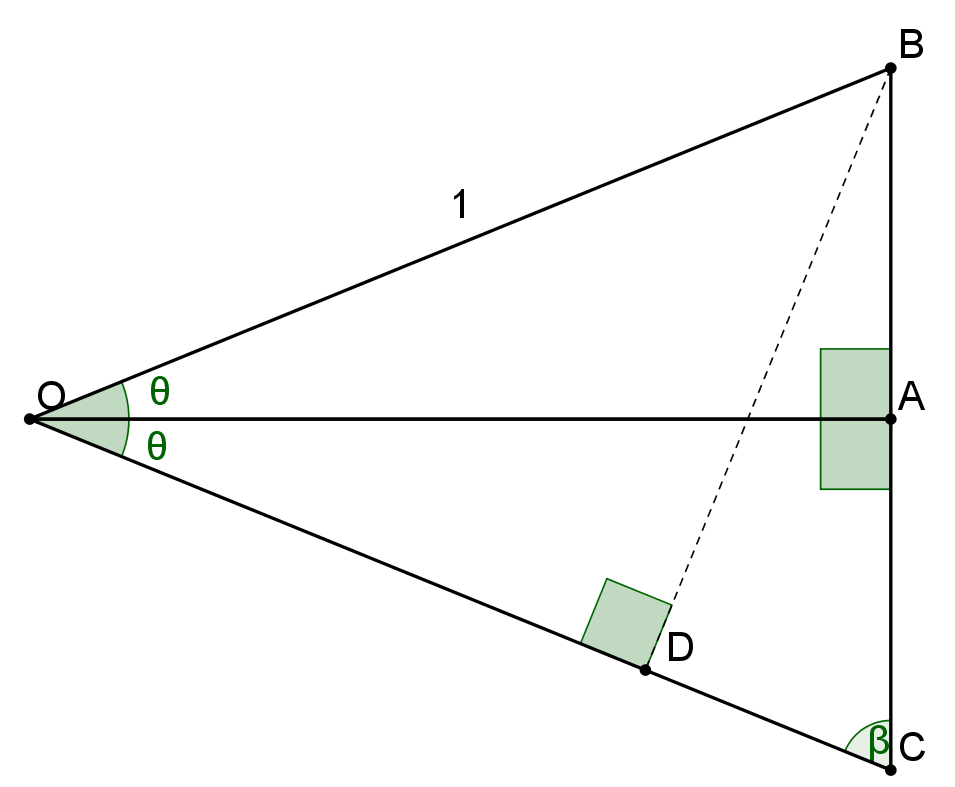
\includegraphics[width=0.8\textwidth]{basic/images/trigo4}
\end{figure}
Esta figura é formada por dois triângulos, $\triangle OAB$ e $\triangle OAC$ congruentes, retângulos em $A$, tais que $\overline{OB}=\overline{OC}=1$ e $A\hat{O}B = A\hat{O}C = \theta$. Nestas condições, temos $\overline{AB}=\overline{AC}=\sin \theta$ e $\overline{OA}=\cos \theta$. Traçando $\overline{BD}$ perpendicular a $\overline{OC}$ temos ainda $\overline{BD}=\sin(2\theta)$. O dobro da área de $\triangle OBC$ é igual a $\overline{BC}\cdot\overline{OA}$ e também igual a $\overline{OC}\cdot\overline{BD}$. Portanto,
\begin{align*}
\overline{BC}\cdot\overline{OA} &= \overline{OC}\cdot\overline{BD}\\
(\overline{AB} + \overline{AC})\cdot \cos \theta &= 1 \cdot \sin(2\theta) \\
(\sin\theta+\sin\theta)\cos\theta &= \sin(2\theta) \\
2\sin\theta\cos\theta &= \sin(2\theta)
\end{align*}
Observemos que $\overline{OD}+\overline{DC}=1$, ou $1\cdot\cos(2\theta)+\overline{BC}\cdot\cos\beta=1$. Como $\overline{BC}=2\cdot \sin \theta $ e $\cos \beta = \sin \theta$ ($\theta$ e $\beta$ são complementares), temos
\[cos(2\theta)+2\sin(\theta)\cdot\sin(\theta)=1\]
ou ainda, \[\sin \theta = \sqrt{\dfrac{1-cos(2\theta)}{2}}\]
Substituindo $2\theta$ por $\theta$ e consequentemente $\theta$ por $\frac{\theta}{2}$, obtemos a relação procurada.
\end{proof}
\end{prop}
%\chapter{Exponencial}
\begin{df}
Seja $a$ um número real e $n$ um número natural. Potência de base $a$ e expoente $n$ é o número $a^n$, tal que:\[a^0 = 1\]
\[a^n = a^{n-1}\cdot a \textrm{,} \,\forall \, n\textrm{,} \,n \geqslant 1\]
\section{Consequências da definição}
\[a^1 = a^0 \cdot a = 1 \cdot a = a\]
\[a^2 = a^1 \cdot a = a \cdot a\]
\[a^3 = a^2 \cdot a = (a \cdot a) \cdot a = a \cdot a \cdot a\]
temos também, de modo geral, para $p \in \mathbb{N} \textrm{ e } p \geq 2$ que $a^p$ é o produto de $p$ fatores iguais a $a$.
\begin{exemplo}
\[3^0 = 1\]

\end{exemplo}
\end{df}

%\chapter{Logaritmos}
Para simplificar cálculos relacionados a Astronomia e as Grandes Navegações, se desenvolveu a ferramenta dos logaritmos. Acima de tudo, o logaritmo é uma operação inversa a potência: enquanto nas raízes estamos buscando a base, o logaritmo nos fornece o expoente necessário para a base dada obter o resultado.
\begin{df}
Sendo $a$ e $b$ números reais e positivos, com $b \neq 1$, chama-se \emph{logaritmo de b na base a}, o expoente que se deve dar à base $b$ de modo que a potência obtida seja igual à $a$. \\ 

Se $a$, $b$ $\in \mathbb{R}$, $0 < b \neq 1$ e $a > 0$, então \[\log_b a = x \Leftrightarrow a^x = b\] onde $b$ é a base, $a$ é o logaritmando e $x$ é o logaritmo.
\end{df}

\begin{exemplo}
\[\log_5 25 = 2 \textrm{ pois } 5^2 = 25\]
\[\log_8 8 = 1 \textrm{ pois } 8^1 = 8\]
\[\log_3 1 = 0 \textrm{ pois } 3^0 = 1\]
\[\log_3  \dfrac{1} {27} = -3 \textrm{ pois } 3^{-3}= (\dfrac {1} {3})^3 = \dfrac {1}{27}\]
\[\log 10000 = 4 \textrm{ pois } 10^4 = 10000\]
\end{exemplo}
\section{Propriedades}
Temos quatro propriedades que são consequências da definição, acompanhe abaixo:

\begin{enumerate}[1.]
\item O logaritmo de $1$ na base $a$ é igual a $0$ para qualquer $a$.\[ \log_a 1 = 0\]
\item logaritmo da base $a$ de $a$ é $1$.\[ \log_a a = 1\]
\item A potência de base $a$ e expoente $\log_a b$  é igual a b.\[ a^{\log_a b} = b \]
A terceira propriedade existe porque o $\log_a b$ é o valor que a base $a$ deve ser elevada para obtermos o logaritmando $b$.
\item Dois logaritmos de uma mesma base são iguais se, e somente se, seus logaritmandos são iguais. \[ \log_a b = \log_a c \Leftrightarrow b = c \]
\end{enumerate}
\section{Sistemas de logaritmos}
O nome \emph{sistemas de logaritmos de base a} se dá ao conjunto de todos os logaritmos dos números reais e positivos em uma base $a$, sendo $0 < a \neq 1$. Como por exemplo o conjunto formado por todos os logaritmos de base 5 dos números reais e positivos é o sistema de logaritmos na base 5.
Dessa infinidade de sistemas de logaritmos, existem dois que são particularmente importantes, o de base 10 e o de base $e$.
O \emph{sistema de base 10} ou \emph{sistema de logaritmos decimais} também é chamado de sistema de logaritmos vulgares ou de Briggs. Indicaremos o logaritmos decimal pela notação $\log_10 x$ ou simplesmente $\log x$.
O \emph{sistema de base $e$ $(e = 2,71828...)$} ou \emph{sistema de logaritmos neperianos} é também chamado de \emph{sistema de logaritmos naturais}. Indicaremos o \emph{sistema de logaritmos naturais} pela notação $\log_e x$ ou $\ln x$.

\section[Operações com Logaritmos]{Propriedades das operações com logaritmos}
Nesta seção veremos algumas propriedades que facilitarão as operações com logaritmos.

\paragraph{Regra do produto}
Em qualquer base $a$ $(0 < a \neq 1)$, o logaritmo do produto de dois fatores reais positivos é igual a soma dos logaritmos dos fatores.
\[\log_a (b.c) = \log_a b + \log_a c\]
Esta propriedade também é válida para $b_n \in \mathbb{R}$, ou seja, $\log_a ( b_1 \cdot  b_2 \cdot  b_3 \cdot \ldots \cdot b_n) = \log_a b_1 + \log_a b_2 + \log_a b_3 + \ldots + \log_a b_n$.

\begin{exemplo}
\[\log_8 \,(5 \cdot 4) = \log_8 5 + \log_8 4\]
\[\log_2 \,(7 \cdot 5 \cdot 6) = \log_2 7 + \log_2 5 + \log_2 6\]\\
\end{exemplo}

\paragraph{Logaritmo do quociente}
Em qualquer base $a$ $(0 < a \neq 1)$, o logaritmo do quociente de dois números reais positivos é igual a diferença entre o logaritmo do dividendo e o logaritmo do divisor.
\[\log_a \dfrac{b}{c} = \log_a b - \log_a c\]
\begin{exemplo}
\[\log_2 \dfrac{5}{8} = \log_2 5 - \log_2 8=\log_2 5 - 3\]
\[\log \dfrac{3 \cdot 4}{7} = \log \,(3 \cdot 4) - \log7= \log 3 + \log 4 - \log 7\]
\[\log \frac{3}{2 \cdot 5} = \log 3\, - \,[\log \,(2 \cdot 5)] = \log 3 \, -\, \log 10 = \log 3\, -\, 1\]\\
\end{exemplo}

\paragraph{Logaritmo da potência}
Em qualquer base $a$ $(0 < a \neq 1)$, o logaritmo de uma potência de base real positiva e expoente real é igual ao produto do expoente pelo logaritmo da base da potência.
\[\textrm{Seja}\, \alpha \in \mathbb{R},\, \textrm{então} \log_a b^{\alpha} = \alpha \cdot \log_a b \]
Em qualquer base $a$ $(0 < a \neq 1)$, o logaritmo da raiz enézima de um número real positivo é igual ao produto do inverso do índice da raiz pelo logaritmo do radicando.
\[\textrm{Seja}\,\, b > 0 \,\,\textrm{e} \,n \in \mathbb{N}^{*}, \,\textrm{então}\, \log_a \sqrt[n]{b} = \log_a b^{\frac{1}{n}} = \frac{1}{n}\log_a b \]
\begin{exemplo}
\[\log_2 5^2 = 2\cdot\log_2 5\]
\[\log_5 \sqrt[3]{2} = \log_5 2^{\frac{1}{3}} = \frac{1}{3}\cdot \log_5 2\]
\[\log_3 \frac{1}{3^4} = \log_3 3^{-4} = -4 \cdot \log_3 3\]
\end{exemplo}
Note que não existem regras para obtermos o logaritmo de uma soma ou diferença, então para encontrarmos $\log_a (b + c)$ e $\log_a (b - c)$ devemos calcular primeiro $(b + c)$ e $(b - c)$.
\paragraph{Mudança de base}
Em certos momentos é conveniente igualarmos as bases de logaritmos para facilitar a solução, como por exemplo na aplicação das propriedades onde os logaritmos devem ter a mesma base. Vejamos o processo que nos permite transformar o logaritmo de um número positivo para outro em uma base conveniente. \par 
Se $a$, $b$ e $c$ são números reais positivos e $a$,\,$c \neq 1$, então temos:
\[\log_a b = \frac{\log_c b}{\log_c a}\]
Esta propriedade também pode ser representada por: \par 
Se $a$, $b$ e $c$ são números reais positivos e $a$,\,$c \neq 1$, então temos:
\[\log_a b = \log_c b \cdot \log_a c\]\\
\begin{exemplo}
\[\log_3 5 \,\, \textrm{transformado para base}\,\, 10 \,\,\textrm{fica:} \]
\[\log_3 5 = \frac{\log 5}{\log 3} \,\,\textrm{ou}\,\, \log_3 5 = \log 5 \cdot \log_3 10 \]
\end{exemplo}

\subsection{Propriedades complementares}
Se $a$ e $b$ são reais positivos e diferentes de $1$, então temos:
\[\log_a b = \frac{1}{\log_b a}\]
Se $a$ $b$ são números reais positivos com $a \neq 1$ e $\beta \in \mathbb{R}^{*}$ então temos:
\[log_{a^{\beta}} b = \frac{1}{\beta}\cdot\log_a b\]
\begin{exemplo}
\[\log_8 3 = \log_{2^{3}} 3 = \frac{1}{3}\cdot \log_2 3\]
\[\log_{\frac{1}{5}} 6 = \log_{5^{-1}} 6 = -\log_5 6\]
\end{exemplo}
\chapter{Matrizes e Sistemas Lineares}

%como chamar a seção que tem a noção de matriz e algumas informações legais de se falar? Definições?
\section{Definições}
Dados dois números naturais não nulos $m,n$, é chamada \emph{matriz m$\times$n} toda tabela com $m$ linhas e $n$ colunas. Se as entradas da tabela forem números reais, esta matriz é dita uma \emph{matriz real m$\times$n}. Neste capítulo iremos trabalhar com matrizes reais.\par 
Em uma matriz $A$ qualquer, seus elementos são simbolizados por $a_{ij}$, onde $i$ é o número da linha e $j$ é o número da coluna deste elemento. As linhas e colunas são numeradas (de $1$ a $m$ ou $n$) conforme a leitura usual: da esquerda para a direita, de cima para baixo, respectivamente. Assim, uma matriz genérica $A_{m\times n}$ é representada por:
\[A_{m\times n}={\begin{bmatrix}
a_{11} & a_{12} & \cdots & a_{1n} \\
a_{21} & a_{22} & \cdots & a_{2n} \\ 
\vdots & \vdots & \ddots & \vdots \\
a_{m1} & a_{m2} & \cdots & a_{mn} 
\end{bmatrix}}\]
Uma matriz do tipo $m \times n$ também pode ser indicada por $A=(a_{ij})_{m\times n}$.
\begin{exemplo}
\[A=(a_{ij})_{3\times 2}=\begin{bmatrix}
1 & -2  \\
2 & 1  \\
3 & 7 
\end{bmatrix}\]
\end{exemplo}

\subsection{Matrizes Especiais}
\subsubsection*{Matriz linha} Uma matriz do tipo $1 \times n$ é chamada matriz linha, pois é uma matriz que tem uma única linha.
\begin{exemplo}
\[L_{5}=\begin{bmatrix} 
-1 & 7 & 3 & 1 & 2 \\
\end{bmatrix}\]
\end{exemplo}
\subsubsection*{Matriz coluna} Uma matriz do tipo $n \times 1$ é chamada coluna, pois é uma matriz que tem uma única coluna.
\begin{exemplo}
\[C_4=\begin{bmatrix} 
2 \\
9 \\
-3 \\
4 
\end{bmatrix}\]
\end{exemplo}

\subsubsection*{Matriz nula} Uma matriz nula é uma matriz que tem todos os elementos iguais a zero.
\subsubsection*{Matriz quadrada de ordem $n$} Chamamos uma matriz $n \times n$ de \emph{matriz quadrada de ordem $n$}, ou seja, uma matriz que tem o mesmo número de linhas e colunas.
\subsubsection*{Matriz diagonal}
Uma matriz onde todos os elementos diferentes de zero estão em sua diagonal principal é chamada \emph{matriz diagonal}.
\paragraph{Diagonal principal} Chamamos de diagonal principal o conjunto de elementos $a_{ij}$ tais que $i=j$.
\paragraph{Diagonal secundária} Chamamos de diagonal secundária o conjunto de elementos $a_{ij}$ tais que $i+j=n+1$.
\subsubsection*{Matriz identidade de ordem $n$} Chamamos de matriz identidade a matriz quadrada e diagonal que possui todos os elementos da diagonal principal iguais a um.
\begin{exemplo}
\[I_{4}=\begin{bmatrix} 
1 & 0 & 0 & 0 \\
0 & 1 & 0 & 0 \\
0 & 0 & 1 & 0 \\
0 & 0 & 0 & 1
\end{bmatrix}\]
\end{exemplo}

\subsection{Igualdade e Operações entre Matrizes}
\[\begin{bmatrix}
a_{11}&\cdots&a_{1n}\\
\vdots&\ddots&\vdots\\
a_{m1}&\cdots&a_{mn}
\end{bmatrix}=\begin{bmatrix}
b_{11}&\cdots&b_{1n}\\
\vdots&\ddots&\vdots\\
b_{m1}&\cdots&b_{mn}
\end{bmatrix}\] Duas matrizes $A_{m\times n},B_{m \times n}$ são ditas iguais se, e somente se, $a_{ij}=b_{ij}$ para todo $i\in \{1,2,\dots,m\}$ e todo $j\in\{1,2,\dots,n\}$. Assim, duas matrizes são ditas iguais se possuem o mesmo tamanho e seus elementos correspondentes são iguais.
\subsubsection{Adição de Matrizes}
\begin{df}
Dadas duas matrizes $A=(a_{ij})_{m \times n}$ e $B=(b_{ij})_{m\times n}$, a matriz \emph{soma} $A+B=(c_{ij})_{m\times n}$, tal que $c_{ij}=a_{ij}+b_{ij}$, para todo $i$ e para todo $j$.
\end{df}
 Assim, a adição é definida entre matrizes de mesmo tamanho e a soma é a matriz (de mesmo tamanho) cujos elementos são a soma dos elementos correspondentes.\par 
A adição de matrizes é associativa, comutativa, possui elemento neutro, todo elemento possui inverso.
\begin{exemplo}
\[\begin{bmatrix}
1 & 0 \\
8 & 1 \\
0 & 4 \\
\end{bmatrix}+\begin{bmatrix}
-1 & 3 \\
0 & 2 \\
-3 & 1
\end{bmatrix}=\begin{bmatrix}
0 & 3 \\
8 & 3 \\
-3 & 5
\end{bmatrix}\]
\end{exemplo}
\subsubsection{Multiplicação de Número por Matriz}
\begin{df}
Dado $k\in \mathbb{R}$ e uma matriz $A=(a_{ij})_{m \times n}$, chama-se o produto $k\cdot A$ a matriz $B=(b_{ij})_{m\times n}$ tal que $b_{ij}=k(a_{ij})$ para todo $i$ e para todo $j$.
\end{df}
Assim, o produto entre um número e uma matriz tem como resultado a matriz de mesmo tamanho, em que todos os elementos são o resultado do produto pelo número.\par 
\begin{exemplo}
\[3\cdot\begin{bmatrix}
1 & -2 & 3 & 0 \\
0 & 1 & -2 & 1
\end{bmatrix}=\begin{bmatrix}
3 & -6 & 9 & 0 \\
0 & 3 & -6 & 3
\end{bmatrix}\]
\end{exemplo}
O produto entre um número e uma matriz é comutativo e possui as seguintes propriedades:
\begin{itemize}
\item $a\cdot (b\cdot A)=(ab)\cdot A$
\item $a\cdot (A+B) = a\cdot A+a\cdot B$
\item $(a+b)\cdot A=a\cdot A+b\cdot A$
\item $1\cdot A=A$
\end{itemize}
\subsubsection{Multiplicação de Matrizes}
\begin{df}
Dadas duas matrizes $A=(a_{ij})_{m \times n}$ e $B=(b_{jk})_{n \times p}$, chama-se produto $AB$ a matriz $C=(c_{ik})_{m\times p}$ tal que \[c_{ik}=a_{i1}b_{1k}+a_{i2}b_{2k}+\cdots +a_{in}b_{nk}=\sum_{j=1}^{n}a_{ij}b_{jk}\]
para todo $i \in \{1,2,3,\dots, m\}$ e para todo $k \in \{1,2,3,\dots, p\}$.
\end{df}
Assim, a multiplicação $AB$ só pode ser realizada se o número de colunas de $A$ for igual ao número de linhas de $B$, e a matriz resultante possui o mesmo número de linhas da matriz $A$ e o número de colunas da matriz $B$. Além disso, o produto pode ser realizado a linha $i$ da matriz $A$ e a coluna $k$ da matriz $B$ para obter o elemento $c_{ik}$ da matriz resultante.
\begin{exemplo}
\[\begin{bmatrix}
1 & 4 & -1 \\
0 & 1 & 2
\end{bmatrix}_{2\times3} \cdot \begin{bmatrix}
1 \\
9 \\
1
\end{bmatrix}_{3\times1}=\begin{bmatrix}
(1\cdot1)+(4\cdot9)+(-1\cdot1)\\
(0\cdot1)+(1\cdot9)+(2\cdot1)
\end{bmatrix}=\begin{bmatrix}
36\\
11
\end{bmatrix}_{2\times1}\]
\end{exemplo}
A multiplicação entre matrizes é associativa, distributiva em relação à adição (à direita e à esquerda) e $(kA)B=k(AB)=A(kB)$, mas não é comutativa e apresenta divisores de zero\footnote{Não é verdade que se $AB=0$, então $A=0$ ou $B=0$, ou seja, nem todo produto de matrizes que resulta na matriz nula envolve uma matriz nula.}.

\subsubsection{Matriz Transposta}
A transposição de matrizes é uma operação unária\footnote{Realizada sobre uma única matriz.} que, intuitivamente, transforma a linha $i$ de uma matriz na coluna $i$, transformando uma matriz $A_{m\times n}$ em uma matriz $A_{n\times m}$.
\begin{df}
Dada uma matriz $A=(a_{ij})_{m\times n}$, chama-se \emph{transposta de $A$} a matriz $A^t=(a'_{ji})_{n\times m}$ tal que $a'_{ji}=a_{ij}$, para todo $i$ e para todo $j$.
\end{df}
\begin{exemplo}
\[\begin{bmatrix}
1 & 1 & 3 \\
0 & 2 & 4
\end{bmatrix}^t= \:
\begin{bmatrix}
1 & 0\\
1 & 2\\
3 & 4
\end{bmatrix}\]
\end{exemplo}

A transposição de matrizes possui as seguintes propriedades:
\begin{itemize}
\item $(A^t)^t=A$
\item $(A+B)^t=A^t+B^t$
\item $(kA)^t=kA^t$
\item $(AB)^t=A^tB^t$
\end{itemize}
\paragraph{Matriz Simétrica}
\begin{df}
Chama-se \emph{matriz simétrica} toda matriz $A$ tal que $A^t=A$. Assim, matrizes simétricas são matrizes quadradas em que $a_{ij}=a_{ji}$, para toda linha $i$ e para toda coluna $j$.  Isto é, $A$ é simétrica se, e somente se, $A^{t} = A$. 
\end{df}
\begin{exemplo}
\[\begin{bmatrix}
0 & 3 & 5 & 7 \\
3 & 0 & 6 & 2 \\
5 & 6 & 0 & 1 \\
7 & 2 & 1 & 0
\end{bmatrix}\]
\end{exemplo}

\subsection{Matrizes Inversíveis}
\begin{df}
Dizemos que uma matriz quadrada de ordem $n$ $A$ é \emph{inversível} se existe $B$ tal que $AB=BA=I_n$. Se $A$ não é inversível, dizemos que $A$ é uma \emph{matriz singular}.
\end{df}
\begin{teo}
Se $A$ é inversível, então é única a matriz $B$ tal que $AB=BA=I_n$.
\begin{proof}
Admitamos que exista $C$ tal que $AC=CA=I_n$. Assim, temos que \[C=I_nC=(BA)C=B(AC)=BI_n=B\]
\end{proof}
\end{teo}
Chamamos a única matriz $B$ tal que $AB=BA=I_n$ de \emph{inversa de $A$} ou $A^{-1}$. \par 
Podemos obter a inversa de $A$ através de sistemas lineares. Como esta resolução é extensa (pois para uma matriz quadrada de ordem $n$, temos de obter $n^2$ incógnitas, resolvendo $n$ sistemas de $n$ equações de $n$ incógnitas cada um), este método será apenas demonstrativo. Segue abaixo um exemplo da resolução.
\begin{exemplo}
\begin{align*}
&A=\begin{bmatrix}
3 & 0 & 1 \\
0 & 1 & 0 \\
2 & 1 & 1
\end{bmatrix} &A^{-1}=\begin{bmatrix}
1 & 1 & -1 \\
0 & 1 & 0 \\
-2 & -3 & 3 
\end{bmatrix} \\ \\
&B=\begin{bmatrix}
1 & 0 \\ -2 & 2
\end{bmatrix} 
&B^{-1}=\begin{bmatrix}
1 & 0 \\
1 & \frac{1}{2}
\end{bmatrix}
\end{align*}
\end{exemplo}

\section{Determinantes}
A teoria dos determinantes foi muito estudada para resolução de sistemas lineares. Atualmente, por não serem um instrumento prático, os determinantes são números vinculados a matrizes, utilizados em demonstrações e para sintetizar certas expressões matemáticas. \par 
O determinante é, também, a área ou o volume determinado entre os vetores dispostos nas colunas da matriz. Disso, decorrem várias das propriedades que trataremos.\footnote{Neste capítulo, traremos uma abordagem algébrica dos determinantes. A parte de Geometria Analítica abordará de forma mais profunda os vetores enquanto entes geométricos.}
A partir de agora, tomaremos $M$ como uma matriz quadrada de ordem $n$.
\subsection{Definições}
\begin{df}
Consideremos uma matriz $M$ de ordem $n\ge 2$; seja $a_{ij}$ um elemento de $M$. Definimos \emph{menor complementar do elemento $a_{ij}$}, e indicamos por $D_{ij}$, o determinante da matriz que se obtém suprimindo a linha $i$ e a coluna $j$ da matriz $M$.
\end{df}
\begin{exemplo}
Dada a matriz \[\begin{bmatrix}
1 & 3 \\
0 & 2
\end{bmatrix}\] determine $D_{21}$. \\ Temos que
\[D_{21}=\begin{Vmatrix}
\not{1} & 3 \\
\not{0} & \not{2}
\end{Vmatrix}=\begin{Vmatrix}
3
\end{Vmatrix}=3\]
\end{exemplo}

\begin{df}
Consideremos uma matriz $M$ de ordem $n \ge 2$; seja $a_{ij}$ um elemento de $M$. Definimos \emph{cofator de $a_{ij}$}, e indicamos por $A_{ij}$, como sendo o número $(-1)^{i+j}\cdot D_{ij}$.
\end{df}
\begin{exemplo}
Determine a matriz dos cofatores de \[A=\begin{bmatrix}
1 & 2 \\
-1 & 0
\end{bmatrix}\]
Para determinar a matriz dos cofatores, precisamos calcular o cofator de cada elemento da matriz. Assim, temos:
\begin{align*}
A_{11}&=(-1)^{1+1}\cdot \begin{Vmatrix}
0
\end{Vmatrix}=0 \\
A_{12}&=(-1)^{1+2}\cdot \begin{Vmatrix}
-1
\end{Vmatrix}=1 \\
A_{21}&=(-1)^{2+1}\cdot \begin{Vmatrix}
2
\end{Vmatrix}=-2 \\
A_{22}&=(-1)^{2+2}\cdot \begin{Vmatrix}
1
\end{Vmatrix}=1
\end{align*}
Assim, a matriz dos cofatores de $A$ é
\[\begin{bmatrix}
0 & -1 \\
2 & 1
\end{bmatrix}\]
\end{exemplo}
\begin{df}
Dada uma matriz quadrada $A$, a \emph{matriz adjunta de $A$}, representada por $\bar{A}$ é a transposta da matriz dos cofatores de $A$.
\end{df}
\begin{exemplo}
Tomando o exemplo anterior, determinaremos a matriz adjunta de $A$ transpondo a matriz dos cofatores. Assim, 
\[\bar{A}=\begin{bmatrix}
0 & 2 \\
-1 & 1
\end{bmatrix} \]
\end{exemplo}
\begin{df}[Teorema Fundamental de Laplace - por recorrência]
Seja $M$ uma matriz de ordem $n$. Definimos o \emph{determinante de $M$}, e denotamos por $\det M$, da seguinte forma:
\begin{enumerate}[i)]
\item Se $n=1$, então $M=\bigl[\begin{smallmatrix}a_{11} \end{smallmatrix}\bigr]$ e $\det M = a_{11}$.
\item Se $n>1$, então $\det M = \displaystyle\sum_{i=1}^{n}a_{ij}\cdot A_{ij}=\displaystyle\sum_{j=1}^{n}a_{ij}\cdot A_{ij}$ ou , ou seja, \emph{o determinante é a soma dos produtos dos elementos de uma fila\footnote{Fila é o nome dado para uma linha ou coluna de uma matriz.} pelos respectivos cofatores}.
\end{enumerate}
\end{df}
\begin{exemplo}
\[\det M=\begin{Vmatrix}
1 & 2 \\
3 & 4
\end{Vmatrix}=(1)(-1)^{1+1}(4)+(3)(-1)^{1+2}(2)=-2\]
\end{exemplo}
\subsubsection{Determinante de Ordem 2}
Para calcular o determinante de uma matriz $M$ de ordem $2$, através da definição, podemos chegar a um método mais simples.
\[\det M=\begin{Vmatrix}
a_{11} & a_{12}\\
a_{21} & a_{22}
\end{Vmatrix}=a_{11}a_{22}-a_{12}a_{21}\]
O determinante é o produto da diagonal principal, subtraindo-se o produto da diagonal secundária.
\subsubsection{Regra de Sarrus}
Se $M$ é de ordem $3$, podemos utilizar a regra de Sarrus para calcular $\det M$. Para isso, copiamos as duas primeiras colunas ao lado da matriz, obtendo assim
\begin{figure}[H]
\centering
\begin{tikzpicture}[>=stealth]
    \matrix [%
      matrix of math nodes,
      column sep=1em,
      row sep=1em
    ] (sarrus) {%
      a_{11} & a_{12} & a_{13} & a_{11} & a_{12} \\
      a_{21} & a_{22} & a_{23} & a_{21} & a_{22} \\
      a_{31} & a_{32} & a_{33} & a_{31} & a_{32} \\
    };
    \path ($(sarrus-1-1.north west)-(0.5em,0)$) edge ($(sarrus-3-1.south west)-(0.5em,0)$)
          ($(sarrus-1-3.north east)+(0.5em,0)$) edge ($(sarrus-3-3.south east)+(0.5em,0)$)
          (sarrus-1-1)              edge            (sarrus-2-2)
          (sarrus-2-2)              edge[->]        (sarrus-3-3)
          (sarrus-1-2)              edge            (sarrus-2-3)
          (sarrus-2-3)              edge[->]        (sarrus-3-4)
          (sarrus-1-3)              edge            (sarrus-2-4)
          (sarrus-2-4)              edge[->]        (sarrus-3-5)
          (sarrus-3-1)              edge[dashed]    (sarrus-2-2)
          (sarrus-2-2)              edge[->,dashed] (sarrus-1-3)
          (sarrus-3-2)              edge[dashed]    (sarrus-2-3)
          (sarrus-2-3)              edge[->,dashed] (sarrus-1-4)
          (sarrus-3-3)              edge[dashed]    (sarrus-2-4)
          (sarrus-2-4)              edge[->,dashed] (sarrus-1-5);

    \foreach \c in {1,2,3} {\node[anchor=south] at (sarrus-1-\c.north) {$+$};};
    \foreach \c in {1,2,3} {\node[anchor=north] at (sarrus-3-\c.south) {$-$};};
  \end{tikzpicture}
\end{figure}
Dessa forma, o determinante é dado pela soma dos produtos das diagonais, onde as três diagonais ``principais'' possuem sinal positivo e as diagonais  ``secundárias'' possuem sinal negativo. Assim, \begin{align*}
\det M =
\underbrace{\bigl[ (a_{11}a_{22}a_{33})+(a_{12}a_{23}a_{31})+(a_{13}a_{21}a_{32})\bigr]}_{\text{Diagonais principais}} \\ -\underbrace{\bigl[(a_{13}a_{22}a_{31})+(a_{32}a_{23}a_{11})+(a_{33}a_{21}a_{12})\big]}_{\text{Diagonais secundárias}}
\end{align*}

\subsection{Propriedades do Determinantes}
Para simplificar o cálculo dos determinantes, podemos utilizar as seguintes propriedades, baseadas na definição 

\begin{prop}[Matriz Transposta]
\[\det M = \det M^t\]
\begin{proof}
Para matrizes de ordem $n=1$, a demonstração é imediata. Suponhamos a propriedade válida para matrizes de ordem $n-1$ e provemos que ela também será válida para matrizes de ordem $n$. Temos:
\[M=\begin{bmatrix}
a_{11} & \cdots & a_{1n} \\
\vdots & \ddots & \vdots \\
a_{n1} & \cdots & a_{nn}
\end{bmatrix} \quad M^t=\begin{bmatrix}
b_{11} & \cdots & b_{1n} \\
\vdots & \ddots & \vdots \\
b_{n1} & \cdots & b_{nn}
\end{bmatrix}\]
em que $b_{ij}=a_{ji}, \forall i,j \in \{1,\dots,n\}$.\\
$\det M =a_{11}A_{11} + a_{21}A_{21}+\dots +a_{n1}A_{n1}$ (pela 1ª linha)\\
$\det M^t =b_{11}B_{11} + b_{21}B_{21}+\dots +b_{n1}B_{n1}$ (pela 1ª coluna)\par 
Mas, por definição de matriz transposta temos: \[a_{11}=b_{11}, a_{21}=b_{12}, \dots, a_{n1}=b_{1n}\] e pela hipótese de indução temos: \[A_{11}=A'_{11}, A_{21}=A'_{12},\dots,A_{n1}=A'_{1n}\]. \par 
Logo, $\det M = \det M^t$
\end{proof}
Tomando esta propriedade, todas as demonstrações a seguir não necessitam ser realizadas para linhas e colunas, ou seja, toda propriedade válida para linhas é automaticamente válida para colunas.
\end{prop}

\begin{prop}[Fila Nula]
Se os elementos de uma fila qualquer de uma matriz $M$ de ordem $n$ forem todos nulos, $\det M =0$.
\begin{proof}
Suponhamos a $j$-ésima coluna de $M$ tenha todos seus elementos nulos. Assim, $a_{1j}=a_{2j}=\dots=a_{nj}=0$. \par 
Tomemos o determinante de $M$ a partir da $j$-ésima coluna. Temos, então:
\[\det M= 0\cdot A_{1j}+0\cdot A_{2j}+\dots +0\cdot A_{nj}=0\]
\end{proof}
\end{prop}

\begin{prop}[Multiplicação de uma Fila por Constante]
Se todos os elementos de uma fila qualquer de uma matriz $M$ de ordem $n$ forem multiplicados por uma constante $k$, então determinante da nova matriz $M'$ será $\det M' = k \det M$.
\begin{proof}
Seja $M=(a_{ij})_{n\times n}$ uma matriz de ordem $n$, e $M'=(b_{ij})_{n\times n}$, onde $b_{ij}=a_{ij}$ se $j \neq t$ e $b_{it}=k\cdot a_{it}$, $t \in \{1,2,\dots,n\}$, ou seja, a $t$-ésima coluna de $M'$ é igual a $k$ vezes a $t$-ésima coluna de $M$. \par 
Os cofatores da $t$-ésima coluna de $M$ são os mesmo da $t$-ésima coluna de $M'$. Tomando o determinante de $M$ e $M'$, temos: \[\det M = a_{1t}A_{1t}+a_{2t}A_{2t}+\dots+a_{nt}A_{nt}\] \[\det M'= k(a_{1t}A_{1t}) + k(a_{2t}A_{2t}) + \dots + k(a_{nt}A_{nt})=k \det M\]
\end{proof}
\end{prop}

\begin{prop}[Filas Paralelas Iguais]
Se uma matriz $M$ possui filas paralelas iguais, ou seja, $\exists j,k$ tais que $a_{ij}=a_{ik}, \forall i$ então $\det M =0$. \par 
Esta propriedade pode ser verificada por meio do conceito de determinante: em uma matriz de ordem 2, temos que o determinante desta matriz $M$ é igual à área do paralelogramo determinado pelos vetores das colunas desta matriz. Assim, se uma matriz possui dois vetores iguais, estes não determinam área, ou seja, $\det M =0$. Caso a matriz seja de ordem 3, temos o volume de um paralelepípedo determinado por três vetores que, se existem dois vetores iguais, não possui uma dimensão, logo não possui volume. Analogamente para matrizes de ordem superior.
%\begin{proof}
%falta
%\end{proof}
\end{prop}

\begin{prop}[Troca de Filas Paralelas]
Quando trocamos filas paralelas de lugar em uma matriz $M$, o determinante da nova matriz $M'$ é $\det M'=-\det M$.
\begin{exemplo}
\begin{align*}
\det(M)=\begin{Vmatrix}
a & b\\
c & d
\end{Vmatrix}&=ad-bc \\
\det(M')=\begin{Vmatrix}
c & d \\
a & b
\end{Vmatrix}&=bc-ad=-(ad-bc)=-\det(M)
\end{align*}
\end{exemplo}
\end{prop}

\begin{prop}[Filas paralelas proporcionais] \marginnote{Esta propriedade é de fácil verificação, utilizando-se das propriedades de filas paralelas iguais e multiplicação de fila por constante.}
Se uma matriz $M$ possui filas paralelas proporcionais, ou seja, $a_{im}=k \cdot a_{in}$ ou $a_{gj}=k \cdot a_{hj}$, para quaisquer $m,n \in \{1,\dots,n\}$ ou quaisquer $g,h \in \{1,\dots,n\}$, $\det M = 0$.
\end{prop}

\section{Sistemas Lineares}
\begin{df}
Chamamos de \emph{equação linear }nas incógnitas $x_1,x_2,x_3,\dots,x_n$ toda equação do tipo $a_{11}x_1+a_{12}x_2+\dots+a_{1n}x_n=b$. \\ Os números reais $a_{11},a_{12},\dots,a_{1n}$ são chamados \emph{coeficientes}, enquanto $b$ é o \emph{termo independente}. \\ Dizemos que uma $n$-upla $(\alpha_1,\alpha_2,\dots,\alpha_n)$ é \emph{solução} de uma equação linear $a_{11}x_1+a_{12}x_2+\dots+a_{1n}x_n=b$ se, e somente se $a_{11}\alpha_1+a_{12}\alpha_2+\dots+a_{1n}\alpha_n=b$ é uma afirmativa verdadeira.
\end{df}
\begin{exemplo}
Seja a equação linear: \[2x_1+3x_2-x_3-2x_4=7\] 
Temos que a $n$-upla $(4,0,7,-3)$ é solução da equação acima, enquanto $(2,5,4,1)$ não é uma solução. \\
Para a equação $0x_1+0x_2+0x_3=4$, podemos claramente ver que não existem soluções, pois a afirmativa será falsa para qualquer $(\alpha_1,\alpha_2,\alpha_3)$.\\
Da mesma forma, qualquer $n$-upla é solução da equação linear $0x_1+0x_2+0x_3=0$.
\end{exemplo}
\begin{df}
Um \emph{sistema linear} é um conjunto de $m$, $m\ge 1$, equações lineares nas incógnitas $x_1,x_2,x_3,\dots,x_n$. Assim, o sistema
\[S=\begin{cases}
a_{11}x_1+a_{12}x_2+\dots+a_{1n}x_n=b_1 \\
a_{21}x_1+a_{22}x_2+\dots+a_{2n}x_n=b_2 \\
\cdots \cdots \cdots \cdots \cdots \cdots \cdots \cdots \cdots\cdots\cdots\\
a_{m1}x_1+a_{m2}x_2+\dots+a_{mn}x_n=b_m\\
\end{cases}\]
Usando a definição de multiplicação de matrizes, podemos escrever o sistema linear acima na forma matricial
\[\underbrace{\begin{bmatrix}
a_{11} & a_{12} & a_{13} & \cdots & a_{1n} \\ 
a_{21} & a_{22} & a_{23} & \cdots & a_{2n} \\ 
\vdots & \vdots & \vdots & \ddots & \vdots \\
a_{m1} & a_{m2} & a_{m3} & \cdots & a_{mn} 
\end{bmatrix}}_{\text{Coeficientes}} \cdot \underbrace{\begin{bmatrix}
x_1 \\
x_2 \\
\vdots \\
x_n
\end{bmatrix}}_{\text{Incógnitas}}=\underbrace{\begin{bmatrix}
b_1 \\
b_2 \\
\vdots \\ 
b_n 
\end{bmatrix}}_{\text{Termos Independentes}}\]
Dizemos que uma $n$-upla é solução de um sistema $S$ se ela é solução de todas as equações do sistema.
\end{df}
\begin{exemplo} Dado o sistema de equações lineares
\[\begin{cases}
-4x+3y=0\\
-5x+6y=18
\end{cases} \text{ou} \quad  \begin{bmatrix}
-4 & 3 \\ -5 & 6
\end{bmatrix}\begin{bmatrix}
x \\ y
\end{bmatrix}=\begin{bmatrix}
0 \\ 18
\end{bmatrix}\] o par ordenado $(x,y)=(6,8)$ é a solução do sistema, enquanto $(3,4)$ não é solução do sistema, pois satisfaz a primeira equação, mas não a segunda. \\
Essa afirmativa é verificável por meio das equações e das matrizes.
\end{exemplo}

\subsection{Discussão de Sistemas Lineares\cite{matriz}} 
Podemos classificar os sistemas lineares quanto as suas soluções. Chamamos isto de \emph{discutir} um sistema linear. Para isso, analisamos as equações para determinar quantas soluções o sistema possui: se ele possui apenas uma solução, se possui infinitas soluções, ou se o sistema não possui soluções.

\[\text{Sistema} \begin{cases}
\text{ Possível}\quad 
	\begin{cases}
	\text{ Determinado} \\
    \\
    \text{ Indeterminado}
	\end{cases}\\
    \\
\text{ Impossível}
\end{cases}\] \par
Um sistema linear é dito \emph{possível} se ele apresenta soluções, ou seja, se $S\neq\emptyset$. Assim, se existe alguma $n$-upla que satisfaz todas as equações do sistema, este sistema é possível. \par 
Se um sistema possível apresenta apenas uma solução, ou seja, $S=\{(\alpha_1,\alpha_2,\dots,\alpha_n)\}$, este sistema é dito um \emph{sistema possível determinado}. Caso o sistema apresente mais de uma solução - infinitas soluções - ele é chamado de \emph{sistema possível indeterminado}. \par 
Um sistema linear que não apresenta soluções, ou seja, $S=\emptyset$ é dito um \emph{sistema impossível}. \par
Tratando geometricamente, podemos utilizar um sistema de duas equações em duas variáveis no plano cartesiano: as equações definem duas retas, e as soluções são a intersecção das retas. Assim, podemos ter retas que se cruzam em um único ponto (sistema possível determinado), retas paralelas, que não se cruzam (sistema impossível) ou retas coincidentes, onde existem infinitas soluções (sistema possível indeterminado). \par 
Para realizar a verificação, podemos utilizar o determinante da matriz $A$ dos coeficientes. Se $\det A \neq 0$, então o sistema é possível e determinado. Se $\det A = 0$, então o sistema é impossível ou indeterminado.

\subsection{Resolução de Sistemas Lineares}
Existem várias técnicas - e teoremas - que podem nos auxiliar a determinar a solução de sistemas lineares. Podemos utilizar a forma matricial para simplificar as equações, para tornas as coordenadas da $n$-upla claras, podemos substituir as equações em outras para reduzir o número de incógnitas, ou até mesmo utilizar determinantes para determinar a solução. Nesta seção, iremos abordar as diferentes formas de determinarmos as soluções de sistemas lineares e as vantagens e desvantagens de cada uma delas.

\subsubsection{Adição}
Quanto trabalhamos com equações lineares de duas - ou até três - incógnitas, é fácil utilizar a técnica da adição. Esta técnica consiste em multiplicar equações do sistema por constantes, de forma que, ao somarmos dada equação do sistema com outra, reduza o número de incógnitas.
\begin{exemplo}
Dadas as equações lineares $3x-5y=6$ e $6x+12y=2$, determine a solução do sistema.
\[\begin{cases}
3x-5y=6 \\
6x+12y=4 \qquad \cdot\left( -\frac{1}{2}\right)
\end{cases} \Rightarrow \begin{cases}
3x-5y=6 \\
-3x -6y = -2
\end{cases}\]
A partir deste sistema, somando as equações, podemos obter a seguinte equação:
\begin{align*}
(3x-5y)+(-3x-6y)&=(6)+(-2) \\ 
-11y&= 4 \\
 y&= -\frac{4}{11}
\end{align*}
Obtendo o valor de uma incógnita, podemos substituir o valor nas equações, reduzindo uma incógnita. Como temos apenas duas incógnitas, a partir do valor de $y$, obtemos diretamente o valor de $x$:
\begin{align*}
3x-5\left(-\frac{4}{11}\right)=&6 \\
3x+\frac{20}{11}=&6 \\
3x=&\frac{66-20}{11}\\
3x=&\frac{46}{11} \\
x=& \frac{46}{33}
\end{align*}
Assim, a solução do sistema é o par ordenado $\left(\frac{46}{33},-\frac{4}{11} \right)$.
\end{exemplo}

\subsubsection{Substituição}
Este método consiste em escrever uma incógnita em função de outras, permitindo a substituição da mesma em outra equação, nos fornecendo o resultado de forma semelhante à adição.
\begin{exemplo}
\[\begin{cases}
4x+2y=14 \\
x-3y=0
\end{cases}\]
Pela segunda equação, sabemos que $x=3y$. Retomando a primeira equação, temos:
\begin{align*}
4x+2y&=14 \\
4(3y)+2y&=14 \\
12y+2y&=14 \\
14y&=14 \\
y&=1
\end{align*}
A partir do valor de $y$, obtemos o valor de $x=3y$.
\begin{align*}
x=&3y\\
x=&3(1)\\
x=&3
\end{align*}
Assim, a solução do sistema é $(3,1)$.
\end{exemplo}
A técnica de substituição é de grande ajuda quando temos uma equação igual a zero.

\subsubsection{Resolução Gráfica}
Quando temos acesso a softwares que geram gráficos, como o GeoGebra ou o GrafEq, é fácil obter a resolução de sistemas de até três variáveis através da intersecção dos planos (ou retas). Esta intersecção é o ponto que satisfaz (pertence aos planos/retas) as equações.
\begin{exemplo}
\[\begin{cases}
3x-y=0 \\
9x+y=36
\end{cases}\]
Cada equação gera uma reta. Aqui temos os gráficos destes planos:  

%arrumar o NODE, TOMÁS
\begin{figure}[H]
\begin{center}
\begin{tikzpicture}
	\begin{axis}[
    	axis x line = center,
        axis y line = center,
        ymin = -10,
        ymax = 10,
        xmin = -10,
        xmax = 10
        ]
		\addplot[mesh,color=red,opacity=0.7]{3*x};
        \addplot[mesh,color=blue,opacity=0.7]{-9*x+36};
        \node[anchor=west] (a) at (axis cs:3,9) {$(3,9)$};
        \node (a) at (axis cs:3,9) {\textbullet};
	\end{axis}
\end{tikzpicture}
\end{center}
\end{figure}

Assim, a intersecção entre os três planos - o ponto que satisfaz as três equações - é o ponto $(3,-1,-1)$.
\end{exemplo}
Mesmo que este método seja o que envolve menos cálculos, só é realmente eficiente com auxilio de um software. Além disso, para utilizar esta técnica em equações lineares com mais de três incógnitas, precisamos reduzir o número de incógnitas - por substituição ou determinando o valor desta incógnita através de outro método específico.


\subsubsection{Teorema de Cramer\cite{fme4}}
O teorema de Cramer é uma forma de resolver sistemas lineares que ``avisa'' se o sistema é determinado ou não antes de grandes cálculos, sendo necessário apenas um determinantes para tal. É uma forma extensa de cálculo para matrizes de ordem maior ou igual a 4.
\begin{teo}
Seja $S$ um sistema linear com número de equações igual ao número de incógnitas e seja $A$ a matriz dos coeficientes de $S$. \\ Se $\det(A)=\Delta\neq 0$, então, o sistema será possível e terá solução única $(\alpha_1,\alpha_2,\dots,\alpha_n)$, tal que
\[\alpha_i= \dfrac{\Delta_i}{\Delta}\]
em que $\Delta_i$ é o determinante da matriz obtida de $A$, substituindo-se a $i$-ésima coluna pela coluna dos termos independentes das equações do sistema.
\end{teo}
\begin{exemplo}
\[\begin{cases}
3x+2y=4
x-y=5
\end{cases}\]
A partir da matriz dos coeficientes, obtemos o valor de $\Delta$.
\[\Delta=\begin{Vmatrix}
3 & 2 \\
1 & -1
\end{Vmatrix}=(-3) - (2)=-5\]
Como $\Delta \neq 0$, sabemos que o sistema é possível e determinado. Assim, encontramos $\Delta_x$ e $\Delta_y$ para resolver o sistema.
\begin{align*}
\Delta_x=&\begin{Vmatrix}
4 & 2 \\
5 & -1
\end{Vmatrix}=(-4)-(10)=-14 \\
\Delta_y=&\begin{Vmatrix}
3 & 4 \\
1 & 5
\end{Vmatrix}=(15)-(4)=11
\end{align*}
Portanto, temos que
\begin{align*}
x=\dfrac{\Delta_x}{\Delta}&=-\dfrac{14}{5}\\
y=\dfrac{\Delta_y}{\Delta}&=\dfrac{11}{5}
\end{align*}
ou seja, $\left(-\dfrac{14}{5},\dfrac{11}{5}\right)$ é a solução do sistema.
\end{exemplo}
Podemos utilizar o teorema de Cramer para discutir um sistema linear. 
\[\begin{cases}
\Delta \neq 0 \Rightarrow \textrm{(SPD)}\\
\\
\Delta = 0 \begin{cases}
\Delta_1=0 \Rightarrow \textrm{(SPI)}\\
\Delta_1 \neq 0 \Rightarrow \textrm{(SI)}
\end{cases}
\end{cases}\]

\subsubsection{Escalonamento}
Para utilizarmos a técnica da adição em sistemas maiores, foi desenvolvido o escalonamento, que consiste em trabalhar com adições e produtos por constantes na matriz dos coeficientes. \par 
\begin{df}
Dado um sistema linear em que cada equação existe pelo menos um coeficiente não nulo, dizemos que $S$ está na \emph{forma escalonada} se o número de coeficientes nulos, antes do primeiro coeficiente não nulo, aumenta de equação para equação.
\end{df}
\begin{exemplo}
\begin{align*}
S_1&=\begin{cases}
3x_1+4x_2-x_3=0 \\
	 5x_2+x_3=3 \\
		 8x_3=1
\end{cases}  &A_1=\begin{bmatrix}
3 & 4 & -1 \\
0 & 5 & 1 \\
0 & 0 & 8
\end{bmatrix} \\
S_2&=\begin{cases}
x=0\\
2y=1\\
4z=7
\end{cases}  &A_2=\begin{bmatrix}
1 & 0 & 0 \\
0 & 2 & 0 \\
0 & 0 & 4
\end{bmatrix} \\
S_3&=\begin{cases}
x+4y-z+w=0 \\
y+2z-3w=3\\
z-w=-15
\end{cases} &A_3=\begin{bmatrix}
1 & 4 & -1 & 1 \\
0 & 1 & 2 & -3 \\
0 & 0 & 1 & -1
\end{bmatrix}
\end{align*}\end{exemplo}
Repare que a matriz dos coeficientes de um sistema escalonado é uma matriz triangular, onde todos os elementos abaixo da diagonal principal são iguais a zero. \par
Para obter a solução de um sistema escalonado, existem dois casos: quando o número de equações é igual ao número de incógnitas, ou quando o número de equações é menor do que o número de incógnitas. \par 
Se o número de equações é igual ao número de incógnitas, temos, pelo teorema de Cramer, que $\det A= a_{11}\cdot a_{22}\cdot \dots \cdot a_{nn} \neq 0$. Portanto, o sistema é possível e determinado, e podemos realizar a substituição a partir da última equação. \par 
Um sistema escalonado com número de incógnitas maior  do que o número de equações é indeterminado, e acaba se tornando um ``sistema-função'': podemos tomar as \emph{variáveis livres} (as incógnitas que não aparecem no começo de nenhuma das equações) e transpô-las para o segundo membro, junto com o termo independente. Assim, podemos atribuir valores para as variáveis livres e definir infinitos sistemas possíveis e determinados. Logo, o sistema original é indeterminado. Chamamos de \emph{grau de indeterminação} o número de variáveis livres do sistema.\par 
Para realizar o escalonamento de um sistema, devemos tomar a \emph{matriz completa}, a matriz formada pela matriz dos coeficientes, com a coluna de termos independentes, para que as operações realizadas não alterem as equações do sistema linear.
\begin{exemplo}
\begin{align*}
&S=\begin{cases}
x+y+z=3 \\
x+2y-z=2 \\
2x-3y+z=0
\end{cases} &M_S=\begin{bmatrix}
1 & 1 & 1 & \vdots & 3 \\
1 & 2 & -1 & \vdots & 2 \\
2 & -3 & 1 & \vdots & 0
\end{bmatrix}
\end{align*}
Partindo da matriz $M_S$, iremos buscar reduzir os coeficientes abaixo da diagonal principal para 0. Podemos realizar as operações de soma de linhas, troca de linhas e produto de linhas por constante.
\begin{align*}
&\begin{bmatrix}
1 & 1 & 1 & \vdots & 3 \\
1 & 2 & -1 & \vdots & 2 \\
2 & -3 & 1 & \vdots & 0
\end{bmatrix}\Rightarrow &(L_2=L_2-L_1) \\
&\begin{bmatrix}
1 & 1 & 1 & \vdots & 3 \\
0 & 1 & -2 & \vdots & -1 \\
2 & -3 & 1 & \vdots & 0
\end{bmatrix}\Rightarrow &(L_3-L_3-2\cdot L_1) \\
&\begin{bmatrix}
1 & 1 & 1 & \vdots & 3 \\
0 & 1 & -2 & \vdots & -1 \\
0 & -5 & -1 & \vdots & -6
\end{bmatrix}\Rightarrow &(L_3=L_3+5\cdot L_2) \\
&\begin{bmatrix}
1 & 1 & 1 & \vdots & 3 \\
0 & 1 & -2 & \vdots & -1 \\
0 & 0 & -11 & \vdots & -11
\end{bmatrix} &\text{Sistema escalonado}
\end{align*}
A partir de agora, iremos determinar as incógnitas por meio de substituições e equações de uma incógnita. Temos então
\[-11z=-11 \Rightarrow z=1\]
Substituindo o valor de $z$ na próxima equação:
\[y-2=-1 \Rightarrow y=1\]
E, por fim, o valor de $y$ e $z$ na última equação:
\[x+2=3\Rightarrow x=1\]
Portanto, a solução do sistema é a terna $(1,1,1)$. \\ 
Tomando o sistema escalonado, podemos dar continuidade com o método de eliminação de Gauss-Jordan. O método consiste em tornar o pivô (o primeiro coeficiente não nulo) igual a $1$ e todos os elementos da coluna de um pivô devem ser iguais a zero. Assim, partindo do sistema escalonado, temos:
\begin{align*}
&\begin{bmatrix}
1 & 1 & 1 & \vdots & 3 \\
0 & 1 & -2 & \vdots & -1 \\
0 & 0 & -11 & \vdots & -11
\end{bmatrix}\Rightarrow &(L_3 =\frac{-L_3}{11}) \\
&\begin{bmatrix}
1 & 1 & 1 & \vdots & 3 \\
0 & 1 & -2 & \vdots & -1 \\
0 & 0 & 1 & \vdots & 1
\end{bmatrix}\Rightarrow &(L_2 =L_2+2L_3) \\
&\begin{bmatrix}
1 & 1 & 1 & \vdots & 3 \\
0 & 1 & 0 & \vdots & 1 \\
0 & 0 & 1 & \vdots & 1
\end{bmatrix}\Rightarrow &(L_1 =L_1-L_3) \\
&\begin{bmatrix}
1 & 1 & 0 & \vdots & 2 \\
0 & 1 & 0 & \vdots & 1 \\
0 & 0 & 1 & \vdots & 1
\end{bmatrix}\Rightarrow &(L_1 =L_1-L_2) \\
&\begin{bmatrix}
1 & 0 & 0 & \vdots & 1 \\
0 & 1 & 0 & \vdots & 1 \\
0 & 0 & 1 & \vdots & 1
\end{bmatrix}\Rightarrow &(L_1 =L_1-L_2) \\
\end{align*}
Com a eliminação de Gauss %continuar
\end{exemplo}

\begin{df}
Dizemos que a matriz $A$ é \emph{linha-equivalente} a matriz $A'$ se $A'$ for obtida de $A$ por meio de uma sequência finita de \emph{operações elementares sobre linhas}. Estas operações são:
\begin{itemize}
\item Troca de posição de duas linhas
\item Multiplicação de uma linha qualquer por um número $k\neq0$
\item Substituição de uma linha, pela soma desta com outra qualquer.
\end{itemize}
\end{df}
\part{Cálculo Diferencial e Integral}
	\parttoc
\chapter{Funções Reais de Uma Variável}
\Blindtext %discute sobre como isso é util pra vida e tals
\section{Polinomial}
%\blindtext
As funções polinomiais são ótimas ferramentas para avaliar situações de Modelagem, como a área de uma folha de alumínio, o volume que ela pode gerar,  o lucro em função das unidades vendidas, em criptografia ou até para modelar a trajetória de um corpo na Física. Polinômios também podem ser usados para visualizar curvas, e por isso podem ser usados para a construção de montanhas-russas. \par 
Na Matemática, os polinômios são também uma grande ferramenta, pois se comportam de forma semelhante a vários outros conjuntos que podem ser alvo de nosso interesse.

\subsection{Constante}
A função constante é dada pela seguinte equação:
\[f(x)=c\], para $c \in \mathbb{R}$.\par
Ela é um polinômio de grau $0$, e tem a forma de uma reta horizontal que passa pelo ponto $(0,c)$. Por ela ser horizontal, todos pontos contida nessa reta são da forma $(x,c)$.
\begin{figure}[H] 
\centering
	\begin{tikzpicture}
		\begin{axis}[
		axis lines = middle,
        xtick = {-4,-3,...,4},
        ytick = {0,1,...,4},
        ymin = 0,
        ymax = 5, 
        xlabel = $x$,
        ylabel = $y$]
        \addplot[
        domain = -5:5,
        samples = 5,
        ]{3.14};
		\end{axis}
	\end{tikzpicture}
    \caption[Função Constante]{$y=\pi$}
\end{figure}

\subsection{Primeiro Grau}
A função de primeiro grau, também chamada de função da reta, é escrita de tal forma:
\[f(x)=ax+b\] para $a,b\in \mathbb{R}$ e $a \neq 0$.\par
Funções que passam pela origem, ou seja, se $b=0$, são chamadas \emph{funções lineares}. Se $b\neq 0$, são ditas \emph{funções afim}. \par
\paragraph{Coeficiente Angular} O coeficiente angular $a$ da função determina o quão rápido ela cresce ou decresce, portanto ela é responsável pela inclinação da reta. Para determinarmos o coeficiente angular da função, dado dois pontos $(x_1,y_1)$ e $(x_2,y_2)$, podemos usar a formula:\[a=\frac{y_2-y_1}{x_2-x_1}\]
Se tivermos um $a>0$, temos uma função crescente. Se $a<0$, temos uma função decrescente, como mostrado a seguir: 

\begin{figure}[H]
\centering
	\begin{subfigure}[b]{0.35\linewidth}
	\centering
		\begin{tikzpicture}
		\begin{axis}[
		axis lines = middle,
        xtick = {-3,-2,...,3},
        width=\linewidth,
        scale only axis,
        ymin = -4,
        ymax = 4, 
		xmin = -3,
        xmax = 3,
        xlabel = $x$,
        ylabel = $y$]
        \addplot[
        domain = -3:3,
        samples = 100,
        ]{2*x+1};
		\end{axis}
        \end{tikzpicture}
	\caption{$y=2x+1$}
	\end{subfigure}
	\qquad
	\begin{subfigure}[b]{0.35\textwidth}
	\centering
		\begin{tikzpicture}
        \begin{axis}[
		axis lines = middle,
        xtick = {-3,-2,...,3},
        ymin = -4,
        ymax = 4,
        xmin = -3,
        xmax = 3,
        width=\linewidth,
        scale only axis, 
        xlabel = $x$,
        ylabel = $y$]
        \addplot[
        domain = -3:3,
        samples = 100,
        ]{-3*x+1};
		\end{axis}
		\end{tikzpicture}
	\caption{$y=-3x+1$}
	\end{subfigure}
\caption{Funções Afim}
\end{figure}

\paragraph{Coeficiente Linear} O coeficiente linear $b$ da função determina aonde a função corta o eixo y. Portanto, se tivermos um coeficiente angular $b$, a função $ax+b$ corta o eixo y no ponto $(0,b)$. Dado a função e o gráfico da função, podemos determinar o coeficiente linear de duas formas:
\begin{enumerate}
\item Substituir x por 0, portanto f(x)=b
\item Encontrar onde a reta corta o eixo y
\end{enumerate}
Caso tivermos somente dois pontos, precisamos primeiro determinar o coeficiente angular, e depois substituir-lo na formula padrão do reta
\begin{exemplo}
Determine a equação da reta que passa pelos pontos $(1,2)$ e $(4,8)$.
\begin{align*}
&a=\frac{8-2}{4-1}=\frac{6}{3}=2&
\end{align*}
\begin{align*}
&b=y_1 - ax_1 \quad \textrm{ou} \quad b=y_2 - ax_2& \Rightarrow\\
&b=2 - 2\cdot1 \quad \textrm{ou} \quad b=8 - 2\cdot4 &\Rightarrow\\ 
&b=0 \quad \textrm{ou} \quad b=0 &
\end{align*}
Nota-se que podemos pegar qualquer um dos dois pontos dados para determinar o coeficiente linear. \\
Achando $a$ e $b$, inserimos eles na equação da reta. Então a reta que passa pelo pontos $(1,2)$ e $(4,8)$ é $y=2x$
\end{exemplo}
\paragraph{Função Identidade} A função identidade é um caso especial da função linear. Sua forma é $f(x)=x$. Ela se chama ``identidade'' pois para qualquer valor $p$ de x, temos $y=p$. Portanto cada ponto tem coordenada x e y idênticas. 

\begin{figure}[H] 
\centering
	\begin{tikzpicture}
		\begin{axis}[
		axis lines = middle,
        xtick = {-4,-3,...,4},
        ytick = {-4,-3,...,4},
        xlabel = $x$,
        ylabel = $y$]
        \addplot[
        domain = -5:5,
        samples = 5,
        ]{x};
		\end{axis}
	\end{tikzpicture}
    \caption[Função Identidade]{$y=x$}
\end{figure}

\subsection{Segundo Grau}
Uma função de segundo grau, comumente chamade de função Quadrática, tem a equação:
\[f(x)=ax^2+bx+c\]
para $a,b,c \in \mathbb{R}$ e $a \neq 0$.\par
O gráfico dessa função pode ter duas aparências, uma para $a>0$, e outra para $a<0$: \par

\begin{figure}[H]
\centering
	\begin{subfigure}[b]{0.4\linewidth}
	\centering
		\begin{tikzpicture}
		\begin{axis}[
		axis lines = middle,
        xtick = {-3,-2,...,3},
        width=\linewidth,
        scale only axis,
        ymin = 0,
        ymax = 6, 
		xmin = -3,
        xmax = 3,
        xlabel = $x$,
        ylabel = $y$]
        \addplot[
        domain = -3:3,
        samples = 100,
        ]{2*x^2};
		\end{axis}\
        \end{tikzpicture}
	\caption{$y=2x^2$}
	\end{subfigure}
	\qquad
	\begin{subfigure}[b]{0.4\textwidth}
	\centering
		\begin{tikzpicture}
        \begin{axis}[
		axis lines = middle,
        xtick = {-3,-2,...,3},
        ymin = -6,
        ymax = 0,
        xmin = -3,
        xmax = 3,
        y axis line style = {stealth-},
        every axis y label/.style={at={(current axis.south)},right=2mm},
        width=\linewidth,
        scale only axis, 
        xlabel = $x$,
        ylabel = $y$]
        \addplot[
        domain = -3:3,
        samples = 100,
        ]{(-2)*x^2};
		\end{axis}
		\end{tikzpicture}
	\caption{$y=-2x^2$}
	\end{subfigure}
\caption{Funções Quadráticas}
\end{figure}

\paragraph{Termo Independente} O termo independente na função quadrática é o $c$. Ele determina onde o gráfico corta o eixo y. Na função quadrática genérica, a função corta o eixo y no ponto $(0,c)$
\paragraph{Raízes} Antes de tentar achar as raízes da função quadrática, precisamos primeiro determinar quantas raízes existem. Para isso, usamos o determinante, que chamamos de $\Delta$:
\[\Delta = b^2-4ac\] Depois de determinar o valor de $\Delta$, podemos cair em 3 casos, e cada uma determina quantas raízes existem na função: 
\begin{enumerate}
\item Se $\Delta$ > 0 , temos 2 raízes reais
\item Se $\Delta$ = 0 , temos 1 raiz real
\item Se $\Delta$ < 0 , temos 0 raízes reais.
\end{enumerate}
\par Para determinar as raízes de uma função quadrática, podemos aplicar a formula de Bháskara:
\[x= \frac{-b \pm \sqrt{b^2-4ac}}{2a} \quad \textrm{ou} \quad x= \frac{-b \pm \sqrt{\Delta}}{2a} \]
Por termos um $\pm$, essa formula nos dá dois resultados:
\[x' = \frac{-b + \sqrt{\Delta}}{2a} \quad \textrm{e} \quad x''= \frac{-b - \sqrt{\Delta}}{2a}\]
Quando nós temos 2 raízes reais, esses dois números serão diferentes. Caso tivermos 1 raiz, os dois serão iguais.
%soma/produto?
\begin{exemplo}
Encontre as raízes da função: $y=x^2-1x-12$
\begin{align*}
& \Delta=(-1)^2-4\cdot 1 \cdot (-12) &\Rightarrow\\
& \Delta=(1)-(-48) &\Rightarrow\\
& \Delta=49
\end{align*}
O nosso $\Delta$ é positivo, portanto temos duas raízes positivas reais. Então usando a formula de Bháskara, temos:
\begin{align*}
&x=\frac{-(-1)\pm \sqrt{49}}{2\cdot 1}& \Rightarrow\\
&x=\frac{1\pm 7}{2} & \Rightarrow\\
&x'=\frac{1+7}{2} \quad \textrm{e} \quad x''= \frac{1-7}{2}& \Rightarrow\\
&x'=4 \quad \textrm{e} \quad x''= -3&
\end{align*}
Portanto nossas duas raízes são 4 e -3.
\end{exemplo}


\subsection{Maiores Graus}
Como discutido antes, se tivermos um grau n de uma função, podemos ter no máximo n raízes para tal função.  Podemos achar certas semelhanças entre funções de graus par e ímpar. 

\begin{figure}[H]
\centering
	\begin{subfigure}[b]{0.4\linewidth}
	\centering
		\begin{tikzpicture}
		\begin{axis}[
		axis lines = middle,
        xtick = {-3,-2,...,3},
        ymin = -5,
        ymax = 5,
        xmin = -3,
        xmax = 3,
        width=\linewidth,
        scale only axis, 
        xlabel = $x$,
        ylabel = $y$]
        \addplot[
        domain = -3:3,
        samples = 50,
        ]{x^3};
		\end{axis}\
        \end{tikzpicture}
	\caption{$y=x^3$}
	\end{subfigure}
	\qquad
	\begin{subfigure}[b]{0.4\textwidth}
	\centering
		\begin{tikzpicture}
        \begin{axis}[
		axis lines = middle,
        xtick = {-3,-2,...,3},
        ymin = -5,
        ymax = 5,
        xmin = -3,
        xmax = 3,
        width=\linewidth,
        scale only axis, 
        xlabel = $x$,
        ylabel = $y$]
        \addplot[
        domain = -3:3,
        samples = 50,
        ]{x^5};
		\end{axis}
		\end{tikzpicture}
	\caption{$y=x^5$}
	\end{subfigure}
\caption{Funções de Grau Ímpar}
\end{figure}

Como podemos ver, as funções $x^3$ e $x^5$ são parecidas. Se olharmos para uma função de grau 3 com o máximo possível de raízes (3), e comprar com uma função de grau 5 com suas máximas possíveis raízes (5), ainda podemos ver essa semelhança:

\begin{figure}[H]
\centering
	\begin{subfigure}[b]{0.4\linewidth}
	\centering
		\begin{tikzpicture}
		\begin{axis}[
		axis lines = middle,
        xtick = {-3,-2,...,3},
        ymin = -5,
        ymax = 5,
        xmin = -3,
        xmax = 3,
        width=\linewidth,
        scale only axis, 
        xlabel = $x$,
        ylabel = $y$]
        \addplot[
        domain = -3:3,
        samples = 50,
        ]{(x+2)*(x-2)*(x)};
		\end{axis}\
        \end{tikzpicture}
	\caption{$y=x^3-4x$}
	\end{subfigure}
	\qquad
	\begin{subfigure}[b]{0.4\textwidth}
	\centering
		\begin{tikzpicture}
        \begin{axis}[
		axis lines = middle,
        xtick = {-3,-2,...,3},
        ymin = -5,
        ymax = 5,
        xmin = -3,
        xmax = 3,
        width=\linewidth,
        scale only axis, 
        xlabel = $x$,
        ylabel = $y$]
        \addplot[
        domain = -3:3,
        samples = 50,
        ]{(x+1)*(x-1)*(x-2)*(x+2)*(x)};
		\end{axis}
		\end{tikzpicture}
	\caption{$y=x^5-5x^3+4x$}
	\end{subfigure}
\caption{Funções de Grau Ímpar}
\end{figure}

Podemos ver que para essas funções, %texto

Quanto à funções com grau par, também podemos ver semelhanças:

\begin{figure}[H]
\centering
	\begin{subfigure}[b]{0.4\linewidth}
	\centering
		\begin{tikzpicture}
		\begin{axis}[
		axis lines = middle,
        xtick = {-3,-2,...,3},
        ymin = -5,
        ymax = 5,
        xmin = -3,
        xmax = 3,
        width=\linewidth,
        scale only axis, 
        xlabel = $x$,
        ylabel = $y$]
        \addplot[
        domain = -3:3,
        samples = 50,
        ]{(x+1)*(x-1)};
		\end{axis}\
        \end{tikzpicture}
	\caption{$y=x^2-2x+1$}
	\end{subfigure}
	\qquad
	\begin{subfigure}[b]{0.4\textwidth}
	\centering
		\begin{tikzpicture}
        \begin{axis}[
		axis lines = middle,
        xtick = {-3,-2,...,3},
        ymin = -5,
        ymax = 5,
        xmin = -3,
        xmax = 3,
        width=\linewidth,
        scale only axis, 
        xlabel = $x$,
        ylabel = $y$]
        \addplot[
        domain = -3:3,
        samples = 50,
        ]{(x+1)*(x-1)*(x-2)*(x+2)};
		\end{axis}
		\end{tikzpicture}
	\caption{$y=x^4-5x^2+4$}
	\end{subfigure}
\caption{Funções de Grau Par}
\end{figure}


\section{Exponencial}
\begin{df}
 Sendo $a\in \mathbb{R}_+^*-\{1\}$, uma função exponencial $f(x)$ é escrita como:
 \[f(x)=a^x\]
\end{df}
Toda função exponencial tem tais características:
\begin{enumerate}
\item $y>0$, portanto nunca corta o eixo x
\item Quando $x=0$, para qualquer $a$, $y=1$
\item Quando $x=1$, $y=a$
\end{enumerate}
Temos 2 casos para funções exponencias, para quando $a>1$ e para $0<x<1$. 

\begin{figure}[H]
\centering
	\begin{subfigure}[b]{0.4\linewidth}
	\centering
		\begin{tikzpicture}
		\begin{axis}[
		axis lines = middle,
        xtick = {-3,-2,...,3},
        width=\linewidth,
        scale only axis,
        ymin = 0,
        ymax = 6, 
		xmin = -3,
        xmax = 3,
        xlabel = $x$,
        ylabel = $y$]
        \addplot[
        domain = -3:3,
        samples = 100,
        ]{2^x};
		\end{axis}\
        \end{tikzpicture}
	\caption{$y=2^x$}
	\end{subfigure}
	\qquad
	\begin{subfigure}[b]{0.4\textwidth}
	\centering
		\begin{tikzpicture}
        \begin{axis}[
		axis lines = middle,
        xtick = {-3,-2,...,3},
        ymin = 0,
        ymax = 6,
        xmin = -3,
        xmax = 3,
        width=\linewidth,
        scale only axis, 
        xlabel = $x$,
        ylabel = $y$]
        \addplot[
        domain = -3:3,
        samples = 100,
        ]{(0.5)^x};
		\end{axis}\
		\end{tikzpicture}
	\caption{$y=(\frac{1}{2})^x$}
	\end{subfigure}
\caption{Funções Exponencias}
\end{figure}

\section{Logarítmica}
\begin{df}
Uma função logarítmica $f(x)$ com base b, para $b>0$ e $b \neq 1$, é escrita de tal forma:
\[f(x)=\log_b x\]
\end{df}
Em geral, toda função logarítmica:
\begin{enumerate}
\item tem $x>0$, portanto nunca corta o eixo y
\item tem $x=1$, quando $y=0$
\item tem $y=1$, quando $x=b$
\end{enumerate}
Como em funções exponencias, temos 2 casos para funções logarítmicas, quando $b>1$ e quando $0<b<1$.

\begin{figure}[H]
\centering
	\begin{subfigure}[b]{0.4\linewidth}
	\centering
		\begin{tikzpicture}
		\begin{axis}[
		axis lines = middle,
        xtick = {0,1,2,...,6},
        width=\linewidth,
        scale only axis,
        ymin = -1,
        ymax = 1, 
        xlabel = $x$,
        ylabel = $y$]
        \addplot[
        domain = 0:7,
        samples = 100,
        ]{log10(x)};
		\end{axis}\
        \end{tikzpicture}
	\caption{$y=\log_{10} x$}
	\end{subfigure}
	\qquad
	\begin{subfigure}[b]{0.4\textwidth}
	\centering
		\begin{tikzpicture}
        \begin{axis}[
		axis lines = middle,
        xtick = {0,1,2,...,6},
        ymin = -1,
        ymax = 1,
        width=\linewidth,
        scale only axis, 
        xlabel = $x$,
        ylabel = $y$]
        \addplot[
        domain = 0:7,
        samples = 100,
        ]{-log10(x)};
		\end{axis}\
		\end{tikzpicture}
	\caption{$y=\log_\frac{1}{10}x$}
	\end{subfigure}
\caption{Funções Logarítmicas}
\end{figure}

\section{Raiz} %applets
Uma função de raiz tem a forma: $\sqrt[a]{x}$, onde $a \in \mathbb{N}$ e $a>1$. \par 
A função raiz é a inversa da função potência.\par 
Quando fazemos uma função dessas, podemos escolher o índice da raiz para a função. Dependendo de se escolhermos um índice par ou impar, temos diferentes formas para o gráfico da função.
\subsection{Índice Par}
Uma função raiz de índice par tem a forma: $\sqrt[2k]{x}$, onde $k \in \mathbb{N}^*$. 
\begin{exemplo}
\[f(x)=\sqrt[2]{x}\]
\[f(x)=\sqrt[6]{x}\]
\end{exemplo}
Raízes de índice par tem uma certa restrição no seu domínio, pois não podemos ter uma raiz de índice par de um número negativo. Portanto, o domínio dessa função é: $Df = [0,+\infty[$\par 
Além disso, temos também que a raiz de um índice par de um número pode ser tanto negativo quanto positivo. Nessas funções, usamos, por definição, somente os números positivos. Ou seja, se $y^{2k}=x$ então $y= + \sqrt[2k]{x}$
Aqui estão alguns exemplos dos gráficos de funções de raiz de índice par: 

\begin{figure}[H]
\centering
	\begin{subfigure}[b]{0.4\linewidth}
	\centering
		\begin{tikzpicture}
		\begin{axis}[
		axis lines = middle,
        xtick = {0,1,2,...,6},
        width=\linewidth,
        scale only axis,
        ymin = 0,
        ymax = 6, 
        xlabel = $x$,
        ylabel = $y$]
        \addplot[
        domain = 0:7,
        samples = 100,
        ]{x^(0.5)};
		\end{axis}\
        \end{tikzpicture}
	\caption{$y=\sqrt[2]{x}$}
	\end{subfigure}
	\qquad
	\begin{subfigure}[b]{0.4\textwidth}
	\centering
		\begin{tikzpicture}
        \begin{axis}[
		axis lines = middle,
        xtick = {0,1,2,...,6},
        ymin = 0,
        ymax = 6,
        width=\linewidth,
        scale only axis, 
        xlabel = $x$,
        ylabel = $y$]
        \addplot[
        domain = 0:7,
        samples = 100,
        ]{x^(1/6)};
		\end{axis}\
		\end{tikzpicture}
	\caption{$y=\sqrt[6]{x}$}
	\end{subfigure}
\caption{Funções Raiz de Índice Par}
\end{figure}

\subsection{Índice Impar}
Uma função raiz de índice par tem a forma: $\sqrt[2k+1]{x}$, onde $k \in \mathbb{N}$. 
\begin{exemplo}
\[f(x)=\sqrt[3]{x}\] \vspace{-1.6cm} \[f(x)=\sqrt[7]{x}\]
\end{exemplo}
Raízes de índice ímpar não tem a mesma restrição no seu domínio que as de índice par, pois podemos ter a raiz de índice ímpar de um número negativo. Ela também não tem a restrição da imagem.

\begin{figure}[H]
\centering
	\begin{subfigure}[b]{0.4\linewidth}
	\centering
		\begin{tikzpicture}
		\begin{axis}[
		axis lines = middle,
        width=\linewidth,
        scale only axis,
        xtick = {-4,-3,...,4},
        xmin = -4,
        xmax = 4,
        ymin = -4,
        ymax = 4, 
        xlabel = $x$,
        ylabel = $y$]
        \addplot[
        domain = -4:4,
        samples = 100,
        ]{x/abs(x)*abs(x)^(1/3)};
		\end{axis}\
        \end{tikzpicture}
	\caption{$y=\sqrt[3]{x}$}
	\end{subfigure}
	\qquad
	\begin{subfigure}[b]{0.4\textwidth}
	\centering
		\begin{tikzpicture}
        \begin{axis}[
		axis lines = middle,
        xtick = {-4,-3,...,4},
        xmin = -4,
        xmax = 4,
        ymin = -4,
        ymax = 4,
        width=\linewidth,
        scale only axis, 
        xlabel = $x$,
        ylabel = $y$]
        \addplot[
        domain = -4:4,
        samples = 100,
        ]{x/abs(x)*abs(x)^(1/7)};
		\end{axis}\
		\end{tikzpicture}
	\caption{$y=\sqrt[7]{x}$}
	\end{subfigure}
\caption{Funções Raiz de Índice Impar}
\end{figure}
% coloca y=f(x) nos caption plis, fica tão mais... FUNÇÃO
\section{Racionais Polinomias}
Tendo dois polinômios $P(x)$ e $Q(x)$ com coeficientes reais, funções racionais tem a forma: 
\[y=\dfrac{P(x)}{Q(x)}\]
\begin{exemplo}
\[f(x)= \dfrac{x^2+1}{x^3+x^2+4}\]
\[g(x) = \dfrac{x^2-1}{x^2-1}\]
\end{exemplo}

\marginnote{Se interpretarmos as funções $g$ e $y=1$ como conjuntos de pares ordenados, as funções são diferentes pois o par $(1,1)\not\in g$ e $(1,1) \in c$.}
É importante notar que mesmo podendo simplificar a função $g$, ela não é igual à função constante $c(x)=1$. Podemos ver isso pelo domínio das funções, onde o domínio de $\frac{x^2-1}{x^2-1}$ é $\textrm{Dom }g=\mathbb{R}-\{\pm 1\}$ e $\textrm{Dom }c=\mathbb{R}$.

\section{Trigonométricas}
\blindtext
\subsection{Seno}
\blindtext
\subsection{Cosseno}
\blindtext
\subsection{Tangente}
\blindtext
\subsection{Cossecante}
\blindtext
\subsection{Secante}
\blindtext
\subsection{Cotangente}
\blindtext
\chapter{Taxas de Variação e Limites}
\section{Limites}
Intuitivamente\footnote{Para definições precisas, veja a parte de Análise Matemática.}, dizer que \emph{o limite de $f(x)$ quando $x$ tende a $p$ é $L$} significa que quando os valores de $x$ se aproximam de $p$, os valores de $f(x)$ se aproximam de $L$. Simbolizamos esta relação por
\[\displaystyle\lim_{x \rightarrow p} f(x)=L\]
\begin{exemplo}
\[\displaystyle\lim_{x\rightarrow 4}x^2\]
Temos $f(x)=x^2$ e $x$ tendendo a $4$. Assim, analisamos os valores de $f(x)$ quando $x$ se aproxima de $4$:
\begin{table}[H]
\centering
\begin{tabular}{c|c}
$x$  & $x^2$ \\ \hline
2    & 4     \\
3    & 9     \\
3,5  & 12,25 \\
3,9  & 15,21 \\
3,99 & 15,92
\end{tabular}
\end{table}
Assim, quando $x<4$, $f(x)$ está se aproximando de $16$.
\begin{table}[H]
\centering
\begin{tabular}{c|c}
$x$  & $x^2$ \\ \hline
5    & 25    \\
4,6  & 21,16 \\
4,2  & 17,64 \\
4,01 & 16,08
\end{tabular}
\end{table}
Assim, quando $x>4$, $f(x)$ também está se aproximando de $16$. Portanto, podemos concluir que $\lim_{x \rightarrow 4}x^2=16$.
\end{exemplo}
É importante ressaltar que quando $x$ se aproxima de um valor $p$, ele não é \emph{igual} a $p$, apenas toma valores próximos (e diferentes) de $p$. \par 
\begin{exemplo}
\[\displaystyle\lim_{x\rightarrow 1}\dfrac{x^2-1}{x-1}\]
O domínio desta função é $\mathbb{R}-\{1\}$, ou seja, $f(x)$ não está definida para $x=1$. Assim, para $x\neq1$, $x-1\neq 0$, o que nos possibilita simplificar a função para o cálculo do limite.
\[\displaystyle\lim_{x\rightarrow 1}x+1=2\]
Assim, podemos afirmar que $lim_{x\rightarrow 1}\frac{x^2+1}{x-1}=2$.
\end{exemplo}

\subsection{Leis dos Limites}
Para calcularmos limites, podemos utilizar propriedades de limites para facilitar os cálculos. Para isso, precisamos apenas que os limites existam.
\begin{align*}
&\lim_{x \rightarrow a}f(x) \pm g(x)  = \lim_{x \rightarrow a}f(x) \pm \lim_{x \rightarrow a} g(x) \\
&\lim_{x \rightarrow a}f(x) \cdot g(x) = \lim_{x \rightarrow a}f(x) \cdot \lim_{x \rightarrow a}g(x) \\
&\lim_{x \rightarrow a}\dfrac{f(x)}{g(x)} = \dfrac{\lim_{x \rightarrow a}f(x)}{\lim_{x \rightarrow a}g(x)},\textrm{ se }\lim_{x \rightarrow a}g(x) \neq 0 \\
&\lim_{x \rightarrow a}kf(x)=k\lim_{x \rightarrow a}f(x) \\
&\lim_{x \rightarrow a}f(x)^{m/n}=\left(\lim_{x \rightarrow a}f(x)\right)^{m/n}
\end{align*}

\subsection{Continuidade}
Se tomarmos $f(x)=x+1$, $g(x)=\dfrac{x^2-1}{x-1}$ e $h(x)=\begin{cases} \frac{x^2-1}{x-1} &\textrm{se } x \neq 1 \\ 
1 & \textrm{se } x = 1 \end{cases}$. Os limites de $f(x)$, $g(x)$ e $h(x)$ quando $x$ se aproxima de $1$ são iguais a $2$, mas apenas $f(1)=2=\lim_{x\rightarrow 1}f(x)$. Assim, $f$ é dita \emph{contínua em 1}, enquanto $g$ e $h$ apresentam uma descontinuidade.
\begin{df}
Uma função $f$ é dita \emph{contínua} em um ponto $x=a$ se três condições forem cumpridas:
\begin{enumerate}[i)]
\item $\lim_{x\rightarrow a}=L$
\item $f(a)=A$ ou $a\in Dom f$
\item $f(a)=\lim_{x\rightarrow a}f(x)$
\end{enumerate}
\end{df}
As condições podem ser interpretadas de forma intuitiva como ``explicações'' da necessidade delas na definição:
\begin{enumerate}[i)]
\item A função se aproxima de $L$ para valores de $x$ ``pelos dois lados'', ou seja, para $x$ tendendo a $a^+$ e $x$ tendendo a $a^-$.
\item Existe $f(a)$ - ou seja, $f(x)$ não deixa um ``buraco'' em $x=a$.
\item Não existe salto: $f(x)$ se aproxima do mesmo valor de $f(a)$ quando $x$ se aproxima de $a$.
\end{enumerate}

\subsection{Limites Laterais}
Podemos analisar os limites de $f$ com valores de $x$ de apenas uma direção. Intuitivamente, realizamos isto para determinar os limites acima. Assim, representamos os \emph{limites laterais} por
\[\displaystyle\lim_{x\rightarrow a^+}f(x) \qquad \qquad \displaystyle\lim_{x\rightarrow a^-}f(x)\]
sendo $x\rightarrow a^+$ o \emph{limite pela direita} (valores $x>a$), e $x \rightarrow a^-$ o \emph{limite pela esquerda} (valores $x<a$).\footnote{Podemos interpretar como ``$x$ tendendo a $a$, mas um pouquinho mais que $a$'' ou ``$x$ tendendo a $a$, mas um pouquinho menos que $a$''.}\par 
O \emph{limite bilateral}, ou apenas \emph{limite}, existe apenas se os limites bilaterais existirem e forem iguais.
\begin{exemplo}
\[\displaystyle\lim_{x \rightarrow 0}\dfrac{1}{x}\]
Para obter o limite, calcularemos os limites laterais.
\[\displaystyle\lim_{x \rightarrow 0^-}\dfrac{1}{x}\]
Para valores de $x$ tendendo a $0$ pela esquerda, temos valores cada vez menores de $f(x)$, não obtendo um valor. Assim, $\lim_{x \rightarrow 0^-}\dfrac{1}{x}=-\infty$.
\[\displaystyle\lim_{x \rightarrow 0^+}\dfrac{1}{x}\]
Para valores de $x$ tendendo a $0$ pela direita, temos valores cada vez maiores de $f(x)$, e dizemos que $\lim_{x \rightarrow 0^+}\dfrac{1}{x}=+\infty$.\par 
Como $\lim_{x \rightarrow 0^-}\dfrac{1}{x} \neq \lim_{x \rightarrow 0^+}\dfrac{1}{x}$, dizemos que a função $f(x)=\frac{1}{x}$ não existe limite para $x$ tendendo a $0$.
\end{exemplo}

\subsection{Limites no Infinito}
O símbolo $\infty$ não representa um número real, mas sim a ideia de valores de magnitude muito grande, que crescem ou descrescem ilimitadamente. Assim, quando queremos analisar o comportamento de uma função para valores muito altos (ou muito baixos), analisamos $x \rightarrow \pm \infty$. \par 
Dizemos que $f(x)$ possui limite $L$ quando $x$ tende ao infinito se a função se aproxima de algum número.
\begin{exemplo}
Seja a função $f(x)=3^x$. Assim, analisaremos os limites dessa função no infinito.
\begin{figure}[H]
	\centering
		\begin{tikzpicture}
		\begin{axis}[
		axis lines = middle,
        xtick = {-3,-2,...,3},
        ytick = {0.3,1,3,9},
        ymin = 0,
        ymax = 6, 
		xmin = -3,
        xmax = 3,
        xlabel = $x$,
        ylabel = $y$]
        \addplot[
        domain = -3:3,
        samples = 100,
        ]{3^x};
		\end{axis}
        \end{tikzpicture}
	\caption[Limites no Infinito]{$f(x)=3^x$}
\end{figure}
Para calcularmos os limites, devemos observar o comportamento da função. Quando $x$ assume valores muito grandes, a $f(x)$ também aumenta ilimitadamente. Assim, dizemos que a função é ilimitada.
\[\lim_{x\rightarrow + \infty}3^x = +\infty\]
Utilizando a notação acima, não estamos dizendo que o limite existe, apenas estamos informando que $f(x)$ assume valores muito altos. \par 
Para valores de $x$ muito pequenos, a função também assume valores cada vez mais próximos de $0$. Portanto,
\[\lim_{x\rightarrow - \infty}3^x = 0\]
ou seja, a função $f(x)=3^x$ possui limite para $x$ tendendo a $-\infty$.
\end{exemplo}
Para calcularmos os limites tendendo ao infinito, usamos propriedades semelhantes às dos limites finitos se as funções apresentam limite. Além disso, temos as seguintes propriedades:
\begin{align*}
&\lim_{x\rightarrow \pm \infty}k= k \\
&\lim_{x\rightarrow \pm \infty}\dfrac{1}{x}= 0
\end{align*}

\subsubsection{Limites no Infinito de Funções Racionais}
Quando estivermos determinando o limite de uma função racional quando \\ $x \rightarrow \pm \infty$, podemos observar apenas a maior potência de $x$ que aparece no numerador e no denominador.
\begin{exemplo}
\[\lim_{x \rightarrow +\infty}\dfrac{x^2+3x}{2x^4-5x^3}\]
Para determinarmos esse limite, temos duas formas de considerar. Podemos dividir tanto o numerador quando o denominador pela maior potência de $x$ e, após isso, aplicar as leis dos limites:
\[\lim_{x \rightarrow +\infty}\dfrac{x^2+3x}{2x^4-5x^3}=\lim_{x \rightarrow +\infty}\dfrac{(x^2/x^4)+(3x/x^4)}{(2x^4/x^4)-(5x^3/x^4)}\]
\[\lim_{x \rightarrow +\infty}\dfrac{(x^2/x^4)+(3x/x^4)}{(2x^4/x^4)-(5x^3/x^4)}=\dfrac{0+0}{2-0}=0\]
Esta é uma forma clara de se obter a resolução. Podemos, também, considerar apenas os monômios de maior grau (uma forma mais simples de determinar o limite).
\[\lim_{x \rightarrow +\infty}\dfrac{x^2+3x}{2x^4-5x^3}=\lim_{x \rightarrow +\infty}\dfrac{x^2}{2x^4}=\lim_{x \rightarrow +\infty}\dfrac{1}{2x^2}=0\]
Tomando outra função, podemos calcular os limites da mesma forma:
\[\lim_{x\rightarrow + \infty}\dfrac{2x^3-3x+1}{x^3-2x^2-5}\]
Dividindo o numerador e o denominador pela maior potência de $x$, neste caso $x^3$.
\[\lim_{x\rightarrow + \infty}\dfrac{2x^3-3x+1}{x^3-2x^2-5}=\lim_{x\rightarrow + \infty}\dfrac{(2x^3/x^3)-(3x/x^3)+(1/x^3)}{(x^3/x^3)-(2x^2/x^3)-(5/x^3)}\]
\[\lim_{x\rightarrow + \infty}\dfrac{(2x^3/x^3)-(3x/x^3)+(1/x^3)}{(x^3/x^3)-(2x^2/x^3)-(5/x^3)}=\dfrac{2-0+0}{1-0-0}=2\]
Da mesma forma, tomando a parcela de maior grau, temos:
\[\lim_{x\rightarrow + \infty}\dfrac{2x^3-3x+1}{x^3-2x^2-5}=\lim_{x\rightarrow + \infty}\dfrac{2x^3}{x^3}=\lim_{x\rightarrow + \infty}\dfrac{2}{1}=2\]
\end{exemplo}
\subsection{Limites Infinitos}
Limites infinitos são usados para descrever o comportamento de funções nas quais os valores se tornam arbitrariamente grandes, positivos ou negativos. Este é o caso da função $f(x)=\frac{1}{x}$, quando $x \rightarrow 0^+$. Quando os valores de $x$ se aproximam de $0$ pela direita, temos valores de $f(x)$ cada vez maiores. Descrevemos que a função tende a $\infty$ conforme $x \rightarrow 0^+$. Ainda assim, o limite não existe, nem o número real $\infty$. Isso significa que o limite não existe por que $\frac{1}{x}$ assume valores cada vez maiores quando $x$ se aproxima de $0$ pela direita.
\[\lim_{x \rightarrow 0^+}\dfrac{1}{x}=+\infty\] \par 
Algo semelhante ocorre quando $x \rightarrow 0^-$. Os valores de $f(x)$ ficam cada vez maiores (em módulo) e negativos. Para qualquer valor negativo $-b$, os valores que $f(x)$ pode assumir são ainda menores do que $f(x)$. Assim, escrevemos
\[\lim_{x \rightarrow 0^-}\dfrac{1}{x}=-\infty\]
Novamente, o limite não existe, nem o número real $-\infty$.
\subsection{Assíntotas}
Caso existam, as assíntotas de uma função são retas das quais a função se aproxima. Por exemplo, na função $f(x)=1/x$, os eixos são assíntotas.
\subsubsection{Assíntotas Verticais}
Quando obtemos o $\lim_{x\rightarrow p^-}= \pm \infty$ e $\lim_{x\rightarrow p^+}= \pm \infty$, obtemos uma assíntota vertical: os valores próximos a $p$ se aproximam de uma reta $x=p$, onde a função é indefinida.
\begin{exemplo}
EXEMPLO DE ASSÍNTOTAS VERTICAIS % GRAFICOS, TOMÁS
\end{exemplo}

\subsubsection{Assíntotas Horizontais}
Assíntotas horizontais são retas das quais os valores de uma função se aproximam quando $x$ se afasta de zero, ou seja, $x \rightarrow \pm \infty$. Assim, podemos ter assíntotas horizontais à esquerda ($x\rightarrow - \infty$) ou à direita ($x\rightarrow + \infty$).
\begin{exemplo}
EXEMPLO DE ASSÍNTOTA HORIZONTAL
\end{exemplo}

\section{Taxas de Variação}
Iniciaremos o estudo sobre taxas de variação tomando o exemplo da velocidade média: a variação do deslocamento em relação ao tempo. \par 
A velocidade média de um corpo em movimento durante um intervalo de tempo é obtida pela razão entre o deslocamento pelo tempo gasto. Assim, sendo $s$ o deslocamento (em metros) e $t$ o tempo gasto (em segundos), a velocidade média é obtida por:
\[V_m=\dfrac{\Delta s}{\Delta t}=\dfrac{s_f-s_i}{t_f-t_i}\] \par 
Geometricamente, a velocidade média pode ser encarada como o coeficiente angular da reta que passa pelos pontos $(t_i,s_i)$ e $(t_f,s_f)$. Portanto é uma boa estimativa de valores, mas pode ser muito imprecisa, dependendo do intervalo de tempo (neste caso a variável livre, ou no eixo das abscissas). Para identificar variações mais precisas, devemos reduzir o intervalo. \par 
Com base no conceito acima, estudaremos as taxas de variações de quaisquer funções reais.
\begin{exemplo}
Analise a variação média entre os pontos $(0,0)$ e $(\pi, \pi)$ no gráfico abaixo.
\begin{figure}[H] 
\centering
	\begin{tikzpicture}
		\begin{axis}[
		axis lines = middle,
        ymin = 0,
        xmin = 0,
        ymax = 6.28,
        xmax = 6.28,
        ytick = {0,1.57,3.1415,4.71,6.28},
        yticklabels = {$0$,$\frac{\pi}{2}$,$\pi$,$\frac{3\pi}{2}$,$2\pi$},
        xtick = {0,1.57,3.14,4.71,6.28},
        xticklabels = {$0$,$\frac{\pi}{2}$,$\pi$,$\frac{3\pi}{2}$,$2\pi$},
        xlabel = $x$,
        ylabel = $y$]
        \addplot[
        domain = -2:3.14,
        samples = 100,
        ]{x-ln(x)*sin(deg(x))};
        \addplot[
        dashed,
        domain = 3.14:6.28,
        samples = 100,
        ]{x-ln(x)*sin(deg(x))};
        \addplot[
        color = red,
        dashed,
        domain = 0:3.14,
        samples = 100
        ]{x};
        \addplot[
        dashed,
        samples=50, 
        domain=0:6,
        ] coordinates {(3.14,0)(3.14,3.14)};
        \addplot[
        dashed,
        domain = 0:3.14,
        samples = 100
        ]{3.14};
		\end{axis}
	\end{tikzpicture}
    \caption[Variação média]{$f(x)=x-\ln(x)\sin(x)$} 
\end{figure}
Se tomarmos o intervalo $[0, \pi]$, temos que $M = \frac{\pi - 0}{\pi -0}=1$. Ainda assim, podemos ver que a função oscila entre valores maiores e menores do que a reta que passa por esses pontos.
\end{exemplo}
Para identificar a variação instantânea de uma função, devemos tomar o menor valor de $\Delta x$. Para isso, passaremos a utilizar a ideia de derivada.
\chapter{Derivadas}
A \emph{derivada} de uma função $f$ em um ponto $x$ é o coeficiente angular da reta tangente ao gráfico desta função no ponto $(x, f(x))$.\par Para determinarmos a reta tangente, definimos uma reta secante à função, como a reta em vermelho no gráfico abaixo. A partir da reta secante, reduzimos a \emph{distância incremental} $h$, aproximando os pontos $(x,f(x))$ e $(x+h,f(x+h))$. \par 
Como não podemos definir uma reta por apenas um ponto, tomamos o limite de $h \rightarrow 0$, aproximando os pontos ao máximo.

\begin{figure}[H]
	\centering
		\begin{tikzpicture}
		\begin{axis}[
		axis lines = middle,
        ytick = {0.48168,0.73146},
        yticklabels = {$f(x)$,$f(x+h)$},
        xtick = {0.13814,0.49277},
        xticklabels = {$x$,$x+h$},
        ymin = 0,
        restrict y to domain = 0:2,
        ymax = 1, 
		xmin = 0,
        xmax = 1,
        xlabel = $x$,
        ylabel = $y$]
        \addplot[
        domain = 0:2,
        samples = 100,
        ]{((4*(x+0.033)-1.126)^7)/3.5+0.01*(x-1.09)+0.49};
        \addplot[ %secante
        domain = 0:2,
        samples = 3,
        olive!40!lime,
        thick,
        ]{0.704*x+0.3843};
        \addplot[
        domain = 0:0.13814,
        samples = 100,
        dashed
        ]{0.48168};
        \addplot[  %ponto (x+h,f(x+h))
        domain = 0:0.49277,
        samples = 3,
        dashed
        ]{0.73146};
        \addplot[
        dashed,
        samples=3, 
        domain=0:6,
        ] coordinates {(0.49277,0)(0.49277,0.73146)};        
        \addplot[ %ponto (x, f(x))
        domain = 0:0.13814,
        samples = 3,
        dashed
        ]{0.48168};
        \addplot[
        dashed,
        samples=3, 
        domain=0:6,
        ] coordinates {(0.13814,0)(0.13814,0.48168)};
		\end{axis}
        \end{tikzpicture}
\end{figure}

\begin{df}
Sejam $f$ uma função. A \emph{derivada} da função $f$ é chamada $f'$ e definida por
\[f'(x)=\displaystyle\lim_{h\rightarrow 0}\dfrac{f(x+h)-f(x)}{h}\] desde que exista o limite. \\
A \emph{reta tangente} à curva $f$ em $(a,f(a))$ é a reta que passa por $(a,f(a))$ e tem coeficiente angular $f'(a)$.
\end{df}
A equação da reta tangente em um ponto $x=p$ é dada por $(y-y_p)=f'(p)(x-x_p)$.

\begin{exemplo}
Dada $f(x)=x^2$, determine a reta tangente a $f$ no ponto de $x=2$. \par 
Para isso, iremos utilizar a definição de derivada:
\begin{align*}
\lim_{h\rightarrow0}\dfrac{(2+h)^2-(2)^2}{h} &= \lim_{h\rightarrow0}\dfrac{(4+4h+h^2)-(4)}{h} \\
&= \lim_{h\rightarrow0}\dfrac{(4h+h^2)}{h} \\
&= \lim_{h\rightarrow0}\dfrac{4+h}{1} \\
f'(2)&= 4
\end{align*}
Para encontrarmos a equação da reta tangente, usaremos $f(2)=2^2=4$. Assim, temos:
\begin{align*}
(y-y_p)&=f'(p)(x-x_p) \\
y-4&=4(x-2) \\
y-4 &=4x-8 \\
y &= 4x-4
\end{align*}
Dada $g(x)=\frac{1}{x}$, determine a inclinação reta tangente no ponto $x=2$. \par 
Novamente, utilizaremos a definição:
\begin{align*}
\lim_{h\rightarrow0}\dfrac{\frac{1}{2+h}-\frac{1}{2}}{h}=&\lim_{h\rightarrow0}\dfrac{1}{h}\cdot\dfrac{2-(2+h)}{2(2+h)} \\
=&\lim_{h\rightarrow0}\dfrac{-h}{2h(2+h)} \\
=&\lim_{h\rightarrow0}\dfrac{-1}{2(2+h)} \\
=&\lim_{h\rightarrow0}\dfrac{-1}{4+2h} \\
g'(2)=&\dfrac{-1}{4}
\end{align*}
\end{exemplo} \par 
Podemos, também, visualizar a derivada como uma função.
\begin{exemplo}
Determine a função $f'(x)$ que fornece o coeficiente angular da reta tangente aos pontos da função definida por $f(x)=3x^2$. \par
Para isso, basta não atribuirmos valores a $x$.
\begin{align*}
\lim_{h\rightarrow0}\dfrac{3(x+h)^2-3(x)^2}{h}=&\lim_{h\rightarrow0}\dfrac{3(x^2+2xh+h^2)-3x^2}{h} \\
=&\lim_{h\rightarrow0}\dfrac{{3x^2}+6xh+3h^2-{3x^2}}{h} \\
=&\lim_{h\rightarrow0}\dfrac{6xh+3h^2}{h} \\
=&\lim_{h\rightarrow0}\dfrac{6x+h}{1} \\
f'(x)=&6x
\end{align*}
Com a função $f'(x)=6x$, podemos determinar facilmente o coeficiente angular da reta tangente a $f$ para qualquer ponto do domínio de $f$.
\end{exemplo} \par 
Podemos utilizar uma versão equivalente da definição de derivada, que pode facilitar o cálculo:
\[\lim_{z\rightarrow x}\dfrac{f(z)-f(x)}{z-x}\]

\section{Funções Diferenciáveis}
\begin{df}
Uma função $y=f(x)$ será \emph{diferenciável} em um intervalo aberto (finito ou infinito) se tiver uma derivada em cada ponto do intervalo. Será diferenciável em um intervalo fechado $[a,b]$ se for diferenciável no intervalo $(a,b)$ e se os limites
\[\lim_{h\rightarrow 0^+}\dfrac{f(a+h)-f(a)}{h} \qquad \textbf{Derivada à direita em a}\]
\[\lim_{h\rightarrow 0^-}\dfrac{f(b+h)-f(b)}{h} \qquad \textbf{Derivada à esquerda em b}\]
existirem nas extremidades do intervalo.
\end{df} \par
As derivadas à direita e à esquerda podem ser definidas em qualquer ponto do domínio, mas são especialmente interessantes para determinar se a função é diferenciável em um intervalo fechado. Por isso, não iremos trabalhar com exemplos de derivadas laterais. \par 
Resumindo a definição, temos que funções são diferenciáveis no domínio de sua derivada.
\subsection{Pontos não-diferenciáveis}
Uma função possui derivada quando possui o limite do coeficiente angular da reta tangente. Quando as retas secantes não apresentam um limite (que resultaria na derivada) ou se tornam verticais a medida que $h \rightarrow 0$, a derivada não existe. Assim, a diferenciabilidade de uma função depende da ``suavidade'' do gráfico da função.
\paragraph{Bico} Ponto contínuo do domínio onde as derivadas laterais são diferentes.
\paragraph{Ponto Cuspidal} Onde o coeficiente angular tende a $\infty$ por um lado e $-\infty$ por outro.
\paragraph{Tangente Vertical} Onde o coeficiente angular tende a $\infty$ (ou $-\infty$) por ambos os lados.
\paragraph{Descontinuidade} A função apresenta uma descontinuidade no ponto.

\begin{teo}\marginnote{Devemos tomar cuidado com a recíproca deste teorema. Nem toda função contínua em um intervalo é diferenciável neste intervalo. Por exemplo, $f(x)=\sqrt[3]{x^2}$, contínua em $\mathbb{R}$, cuja derivada $f'(x)=\frac{2}{3\sqrt[3]{x}}$ não existe no ponto $x=0$).}
Se $f$ tem uma derivada em $x=c$, então $f$ é contínua em $x=c$.
\begin{proof}
Como $f'(c)$ existe, devemos mostrar que $\lim_{x\rightarrow c}f(x)=c$ ou, de maneira equivalente, que $\lim_{h\rightarrow 0}f(c+h)=f(c)$. Se $h\neq0$, então
\begin{align*}
f(c+h)=&f(c)+(f(c+h)-f(c))\\
=&f(c)+\dfrac{\left[f(c+h)-f(c)\right]}{h}\cdot h
\end{align*}
Agora, tomando o limite quando $h \rightarrow 0 $, temos
\begin{align*}
\lim_{h\rightarrow0}f(c+h)=&\lim_{h\rightarrow0}f(c)+\lim_{h\rightarrow0}\dfrac{f(c+h)-f(c)}{h}\cdot \lim_{h\rightarrow0}h \\
=&f(c)+f'(c)\cdot0\\
=&f(c)
\end{align*}
Assim, se uma função possui derivada em um ponto, a função é contínua no ponto.
\end{proof}
\end{teo}

\section{Regras de Derivação}
Para evitar a aplicação da definição em derivadas, foram desenvolvidas certas regras para tornar o processo mais rápido. Estas regras permitem derivar uma grande variedade de funções, como as polinomiais, trigonométricas, produtos e quocientes. Além disso, todas as regras aqui apresentadas podem ser demonstradas a partir da definição. \par Utilizaremos $c$ como uma constante qualquer e $u,v$ como funções de $x$ para evitar confusão com $f$ e $g$.

\subsection{Polinomiais}
\begin{align*}
\dfrac{d}{dx}(c)&=0 \\ \dfrac{d(x)}{dx}&=1 \\ \dfrac{d}{dx}(x^n)&=nx^{n-1}, \: \forall n \neq 0 \\ \dfrac{d}{dx}\left(c\cdot u\right)&=c\cdot \left(\dfrac{du}{dx}\right) \\ \dfrac{d}{dx}(u\pm v)&=\dfrac{du}{dx}\pm \dfrac{dv}{dx} \\ 
\end{align*}
\begin{exemplo}
\begin{align*}
f(x)=3x^2+10 \Rightarrow \dfrac{df}{dx}&=\dfrac{d}{dx}(3x^2+10)\\ &=\dfrac{d}{dx}(3x^2)+\dfrac{d}{dx}(10) \\ &=3\dfrac{d}{dx}(x^2)+0 \\ &=3\cdot 2x^{2-1}\\ &=6x
\end{align*}
\begin{align*}
\dfrac{d(\sqrt[3]{x})}{dx}&=\dfrac{d(x^{\frac{1}{3}})}{dx}\\
&=\dfrac{1}{3}x^{\frac{1}{3}-1}\\
&=\dfrac{x^{-\frac{2}{3}}}{3}\\
&=\dfrac{1}{3\sqrt[3]{x^2}}
\end{align*}
\end{exemplo}

\subsection{Produto e Quociente}
\begin{align*}
\dfrac{d}{dx}(uv)&=u\dfrac{dv}{dx}+v\dfrac{du}{dx}\\
\dfrac{d}{dx}\left(\dfrac{u}{v}\right)&=\dfrac{v\frac{du}{dx}-u\frac{dv}{dx}}{v^2}
\end{align*}
\begin{exemplo}
\begin{align*}
g(x)&=(3x^2-5)(x^3+2x) \\ \dfrac{dg}{dx} &=\dfrac{d}{dx}(3x^2-5)\cdot (x^3+2x) + \dfrac{d}{dx}(x^3+2x) \cdot (3x^2-5) \\
&=(6x)(x^3+2x)+(3x^2+2)(3x^2-5) \\
&= 6x^4+12x^2+9x^4-15x^2+6x^2-10 \\
&= 15x^4+3x^2-10
\end{align*}
\begin{align*}
f(x)=\dfrac{3x}{x^2+1} \Rightarrow \dfrac{df}{dx}&=\dfrac{d}{dx}\left(\dfrac{3x}{x^2+1}\right)\\
&=\dfrac{(x^2+1)\cdot\frac{d}{dx}(3x)-3x\cdot\frac{d}{dx}(x^2+1)}{(x^2+1)^2}\\
&=\dfrac{3\cdot(x^2+1)-3x\cdot(2x)}{(x^2+1)^2} \\
&=\dfrac{3x^2+3-6x^2}{(x^2+1)^2} \\
&=\dfrac{-3x^2+3}{(x^2+1)^2}
\end{align*}
Tomemos a função $y=1/x$. Repare que podemos resolvê-la de duas formas, obtendo o mesmo resultado:
\begin{align*}
\dfrac{dy}{dx}&=\dfrac{d(x^{-1})}{dx}\\ &=-1\cdot x^{-1-1}=-x^{-2}\\ &=-\dfrac{1}{x^2} \\
\textrm{Ou então:}\\
\dfrac{dy}{dx}&=\dfrac{d}{dx}\left(\dfrac{1}{x}\right)\\
&=\dfrac{(1)'(x)-(x)'(1)}{(x)^2}\\
&=-\dfrac{1}{x^2}
\end{align*}
\end{exemplo}

\subsection{Exponencial e Logarítmica}
\begin{align*}
\dfrac{d}{dx}\log_a x=\dfrac{1}{x\ln(a)} &\Rightarrow \dfrac{d(\ln x)}{dx}=\dfrac{1}{x}\\
\dfrac{d}{dx}(a^x)=a^x \ln(a) &\Rightarrow \dfrac{d(e^x)}{dx}=e^x
\end{align*}
\begin{exemplo}
\begin{align*}
\dfrac{d}{dx}\left(e^x\cdot \ln(x)\right)&=(e^x)'\ln(x) + \left(\ln(x)\right)'e^x\\
&=e^x\ln(x)+\frac{e^x}{x}=e^x\left(\ln(x)+\frac{1}{x}\right)
\end{align*}
\begin{align*}
\dfrac{d}{dx}(xe^x)&=\dfrac{dx}{dx}e^x+\dfrac{d(e^x)}{dx}x\\
&=e^x+x e^x\\
&=e^x(x+1)
\end{align*}
\end{exemplo}

\subsection{Trigonométricas}
\begin{align*}
 \marginnote{Repare que todas as derivadas de funções trigonométricas que iniciam com ``co'' possuem o sinal negativo e ``co'' nas funções trigonométricas da derivada (exceto o cosseno).} \dfrac{d(\sin (x))}{dx}&=\cos(x) \\
\dfrac{d(\cos(x))}{dx}&=-\sin(x) \\
\dfrac{d(\tan(x))}{dx}&=\sec^2(x) \\
\dfrac{d(\cot(x))}{dx}&=-\csc^2(x) \\
\dfrac{d(\sec(x))}{dx}&=\sec(x)\tan(x) \\
\dfrac{d(\csc(x))}{dx}&=-\csc(x)\cot(x) \\
\end{align*}
\begin{exemplo}
\begin{align*}
\dfrac{d}{dx}\tan(x)&=\dfrac{d}{dx}\left(\dfrac{\sin(x)}{\cos(x)}\right)\\
&=\dfrac{\cos(x)\frac{d(\sin(x))}{dx}-\sin(x)\frac{d(\cos(x))}{dx}}{(\cos(x))^2}\\
&=\dfrac{\cos^2(x)+\sin^2(x)}{\cos^2(x)}\\
&=\dfrac{1}{\cos^2(x)}\\
&=\sec^2(x)
\end{align*}
\end{exemplo}

\section[Regra da Cadeia]{Funções Compostas}
\begin{exemplo}
Seja $y=f(x)=9x^2-6x+1=(3x-1)^2$. Assim, podemos escrever $f(u)=u^2$, sendo $u=3x-1$. Calculando as derivadas de $\dfrac{dy}{dx}$, $\dfrac{dy}{du}$ e $\dfrac{du}{dx}$, temos:
\begin{align*}
\dfrac{dy}{dx}&=18x-6 \\
\dfrac{dy}{du}&=2u \\
\dfrac{du}{dx}&=3 \\
\dfrac{dy}{du}\cdot \dfrac{du}{dx}&=6u=6(3x-1)=18x-6
\end{align*}

Assim, temos que $\dfrac{dy}{dx}=\dfrac{dy}{du}\cdot \dfrac{du}{dx}$.
\end{exemplo}

\begin{teo}[Regra da Cadeia]
Se $f(u)$ é diferenciável no ponto $u=g(x)$ e $g(x)$ é diferenciável em $x$, então a função composta $(f\circ g)(x)=f(g(x))$ é diferenciável em $x$ e \[(f\circ g)'(x)=f'(g(x))\cdot g'(x)\] Na notação de Leibniz, se $y=f(u)$ e $u=g(x)$, então \[\dfrac{dy}{dx}=\dfrac{dy}{du}\cdot \dfrac{du}{dx}\].
\end{teo}

Após desenvolver as regras práticas para a derivação de funções simples, utilizamos a \emph{Regra da Cadeia} para derivar funções compostas, como $y=\sin(x^2)$, onde temos $y=\sin(u)$ e $u=f(x)$. Para isso, devemos considerar a derivada da função interna (neste caso, $x^2$) e a relação com a derivada da externa (neste caso, $\sin(u)$).
\begin{exemplo}
Resolvendo o exemplo acima:
\begin{align*}
y&=\sin(x^2)\\
\dfrac{dy}{dx}&=\dfrac{dy}{du}\cdot \dfrac{du}{dx}\\
&=\cos(x^2)\cdot 2x\\
&=2x\cos(x^2)
\end{align*}
\end{exemplo}

Podemos, também, lembrar da regra da cadeia como ``deriva a de fora, conservando a de dentro, vezes a derivada da de dentro''. Isso facilita para resolver regras da cadeia com mais de duas funções compostas.
\begin{exemplo}
Seja $y=\sin^2(2x+1)$. Assim, temos $y=u^2$, onde $u=\sin(v)$, sendo $v=2x+1$. Aplicando repetidamente a definição, temos:
\[\dfrac{dy}{dx}=\dfrac{dy}{du}\cdot \dfrac{du}{dv} \cdot \dfrac{dv}{dx}\]
Para resolver, realizamos o mesmo procedimento:
\begin{align*}
y &=\sin^2(2x+1) \\
y' &=2\sin(2x+1) \cdot [ \sin(2x+1)]' \\
y' &=2\sin(2x+1) \cdot \cos(2x+1) \cdot (2x+1)' \\
y' &=2\sin(2x+1) \cdot \cos(2x+1) \cdot 2 \\
y' &=4\sin(2x+1) \cos(2x+1)
\end{align*}
\end{exemplo}

\subsection{Derivação Implícita}
A maioria das funções com que lidamos são da forma $y=f(x)$, onde temos explicitamente $y$ em função de $x$. Quando encontramos equações do tipo $F(x,y)=0$, nem sempre podemos escrevê-las na forma $y=f(x)$ para derivá-la de maneia usual. Ainda assim, podemos determinar $dy/dx$ por intermédio da \emph{derivação implícita}. \par Para isso, simplesmente derivamos ambos os lados da equação em relação a $x$, considerando $y=f(x)$ como uma função diferenciável de $x$.
\begin{exemplo}
Seja a equação $y^2=x$. Esta define duas funções diferenciáveis, $y_1=\sqrt{x}$ e $y_2=-\sqrt{x}$. No entanto, podemos determinar $dy/dx$ sem conhecer estas funções:
\begin{align*}
y^2=x\\
\dfrac{d}{dx}(y^2)=\dfrac{dx}{dx}\\
2y\cdot y' =1\\
y'=\dfrac{1}{2y}
\end{align*}

\begin{center}
	\begin{tikzpicture}
		\begin{axis}[
		axis lines = middle,
        ymin = -3,
		ytick = {-2,-1,...,1,2},
        ymax = 3, 
		xmin = 0,
        xmax = 5.5,
        xlabel = $x$,
        ylabel = $y$]
        \addplot[ %curva superior
        domain = 0:8,
        samples = 150,
        ]{sqrt(x)};
        \addplot[ %curva inferior
        domain = 0:8,
        samples=150,
        ]{-sqrt(x)};        
		\end{axis}
	\end{tikzpicture}
\end{center}
Esta fórmula sozinha fornece as derivadas para as funções explícitas $y_1$ e $y_2$.
\end{exemplo}
Podemos determinar $dy/dx$ facilmente por meio destes três passos a seguir:
\begin{enumerate}[1.]
\item Derive os dois lados da equação em realação a $x$, considerando $y=f(x)$ - ou seja, aplicando a regra da cadeia em $y$.
\item Reúna os termos que contêm $y'=dy/dx$ em um lado da equação.
\item Encontre $dy/dx$.
\end{enumerate}
Podemos utilizar $dy/dx$ determinado implicitamente para encontrar a reta tangente a curva e a \emph{reta normal} a esta. A reta normal é a reta perpendicular a reta tangente no ponto de tangência.
\begin{exemplo}
Seja a curva definida implicitamente pela equação $x^3+y^3-9xy=0$. Determinaremos a reta normal a curva no ponto $(2,4)$.
Assim, precisamos do coeficiente angular da reta, dado por $dy/dx$.
\begin{center}
	\begin{tikzpicture}
		\begin{axis}[
		axis lines = middle,
        ymin = -1,
		ytick = {0,1,2,3,4},
        ymax = 5, 
		xmin = -1,
        xtick = {0,1,2,3,4},
        xmax = 5,
        xlabel = $x$,
        ylabel = $y$,
        width = 0.7\textwidth]
        \addplot[ %reta tangente
        domain = 0:8,
        samples = 2,
        ]{0.8*x+2.4};
        \draw[samples=200,domain=125:-35]plot(\x:{9*sin(\x)*cos(\x)/(sin(\x)^3+cos(\x)^3)}); % AINDA NÃO
        \addplot[ %reta normal
        domain = 0:8,
        samples = 2,
        ]{-1.25*x+6.5};        
		\end{axis}
	\end{tikzpicture}%
\end{center}%
\begin{align*}
x^3+y^3-9xy&=0 \\
\dfrac{d}{dx}(x^3)+\dfrac{d}{dx}y^3 -9 \dfrac{d}{dx}(xy)&=0 \\
3x^2+3y^2y'-9\cdot \left[x\dfrac{dy}{dx}+y\dfrac{dx}{dx}\right]&=0 \\
3x^2+3y^2y'-9\left(xy'+y\right)&=0\\
3x^2+3y^2y'-9xy'-9y&=0\\
3y^2y'-9xy'&=9y-3x^2 \\
y'=\dfrac{9y-3x^2}{3y^2-9x}&=\dfrac{3y-x^2}{y^2-3x} \\
\end{align*}
A partir desta equação, podemos determinar $dy/dx$:
\begin{align*}
y'&=\dfrac{3(4)-(2)^2}{(4)^2-3(2)} \\
y'&=\dfrac{12-4}{16-6}\\
y'&=\dfrac{8}{10}=\dfrac{4}{5}
\end{align*}
Assim, a reta tangente a curva no ponto $(2,4)$ é:
\begin{align*}
y-(4)&=\dfrac{4}{5}(x-2) \\
y&=\dfrac{4x}{5}-\dfrac{8}{5}+\dfrac{20}{5}\\
y&=\dfrac{4x}{5}+\dfrac{12}{5}
\end{align*}
A reta normal a curva em $(2,4)$ é a reta perpendicular a tangente, tendo coeficiente angular igual a $-5/4$:
\begin{align*}
y-(4)&=-\dfrac{5}{4}(x-2) \\
y&=-\dfrac{5x}{4}+\dfrac{10}{4}+\dfrac{16}{4}\\
y&=-\dfrac{5x}{4}+\dfrac{26}{4}\\
y&=-\dfrac{5x}{4}+\dfrac{13}{2}
\end{align*}
\end{exemplo}

\subsection{Funções Parametrizadas}
Uma curva parametrizada $x=f(t)$ e $y=g(t)$ será \emph{diferenciável} em $t$ se $x$ e $y$ forem diferenciáveis em $t$. Em um ponto de uma curva parametrizada diferenciável, onde $y$ também é função diferenciável de $x$, as derivadas $dy/dt$, $dx/dt$ e $dy/dx$ estão relacionadas com a regra da cadeia:
\[\dfrac{dy}{dt}=\dfrac{dy}{dx}\cdot \dfrac{dx}{dt}\]
Se $dx/dt \neq 0 $, então podemos dividir ambos os lados da equação, obtendo então $dy/dx$.
\begin{prop}
Se existirem $dy/dt$, $dx/dt$ e $dy/dx$ e $dx/dt \neq 0$, então
\[\dfrac{dy}{dx}=\dfrac{dy/dt}{dx/dt}\]
\end{prop}
\begin{exemplo}
A reta tangente a circunferência parametrizada por
\begin{align*}
\begin{cases}
x=5\cos(t)\\
y=5\sin(t)
\end{cases} , 0\leq t \leq 2\pi \Rightarrow
\begin{cases}
\cos(t)=x/5 \\
\sin(t)=y/5
\end{cases}
\end{align*}
no ponto $(3,4)$.
\begin{align*}
\dfrac{dx}{dt}&=-5\sin(t)\\
\dfrac{dy}{dt}&=5\cos(t)
\end{align*}
Então,
\begin{align*}
\dfrac{dy}{dx}&=\dfrac{-5\cos(t)}{5\sin(t)}\\
\dfrac{dy}{dx}&=\dfrac{-5(x/5)}{5(y/5)} \\
\dfrac{dy}{dx}&=\dfrac{-x}{y}
\end{align*}
Portanto, o coeficiente angular da reta tangente à circunferência no ponto $(3,4)$ é $-3/4$. A reta tangente é definida por:
\begin{align*}
y&=4-\dfrac{3}{4}(x-3)\\
y&=4-\dfrac{3x}{4}+\dfrac{9}{4} \\
y&=\dfrac{25}{4}-\dfrac{3x}{4}
\end{align*}
\end{exemplo}

\section{Taxas Relacionadas}
Nesta seção estudaremos problemas em que temos que determinar taxas de alguma variável, ampliando nossos conhecimentos de velocidade média do capítulo anterior. Para determinarmos, escrevemos uma equação que relaciona as variáveis envolvidas e a derivamos, buscando assim uma relação entre as taxas.
\begin{exemplo}
Suponha que tenhamos um tanque cilíndrico vertical. A que taxa o nível do líquido diminui se bombearmos o líquido para fora a uma taxa de $3.000 \ell/\min$? \\
Imagine um tanque cilíndrico parcialmente cheio: a quantidade de líquido em seu interior varia, mudando o volume $V$ e o nível $h$ do líquido, mas o raio $r$ permanece constante. Assim, sabemos que $h$ e $V$ são funções diferenciáveis do tempo $t$. Sabemos que \[\dfrac{dV}{dt}=-3.000\] Repare que a taxa é negativa, pois o volume está diminuindo.
Devemos determinar $dh/dt$. Para isso, escrevemos uma equação que relacione o volume do cilindro com sua altura.
\[V=\pi r^2 h\]
Com $V$ em litros e $h$ e $r$ em metros, devemos ajustar a equação:
\[V=1000 \pi r^2 h\]
pois um metro cúbico contém $1.000 \ell$.
A partir dessa relação, temos:
\[\dfrac{dV}{dt}=1000\pi r^2 \dfrac{dh}{dt} \]
Não derivamos $r$ em relação a $t$ pois o raio do cilindro não altera. Assim, podemos substituir os valores conhecidos, neste caso $dV/dt$, e determinamos $dh/dt$:
\begin{align*}
\dfrac{-3000}{1000\pi r^2}=\dfrac{dh}{dt}\\
\dfrac{dh}{dt}=\dfrac{-3}{\pi r^2}
\end{align*}
Sendo assim, o nível do líquido diminui a uma taxa de $dh/dt=(3/\pi r^2) m/\min$. Esta equação mostra como o raio do cilindro se relaciona com a variação do nível do líquido: se o raio for grande, a variação do nível será pequena; se o raio for pequeno, a variação do nível será maior.
\end{exemplo}
A maior parte dos problemas de taxas relacionadas são variações em função do tempo. Assim, existem certas estratégias para a resolução dos problemas de taxas relacionadas:\cite{thomas}
\begin{enumerate}
\item Desenhe uma figura e identifique as variáveis e as constantes. 
\item Escreva as informações numéricas.
\item Escreva aquilo que você deve encontrar.
\item Encontre uma equação que relacione as variáveis.
\item Derive em relação a $t$.
\item Calcule.
\end{enumerate}

\section{Linearização e Diferenciais}
Muitas vezes o cálculo de uma função pode ser complexo, devido a valores muito precisos de $x$ ou funções mais complicadas. Para simplificar estes cálculos, podemos realizar aproximações que funcionam de forma semelhante a arredondamentos: você recebe uma estimativa, que está próxima do resultado real. \par Quando nos aproximamos de um ponto do gráfico de uma função em que a função é derivável, podemos ver que o gráfico se torna mais semelhante a sua tangente. Quando utilizamos a reta tangente como aproximação do gráfico de uma função, chamamos isto de \emph{linearização}
\begin{df}
Se $f$ é diferenciável em $x=a$, então a função aproximação \[L(a)=f(a)+f'(a)(x-a)\] é a \emph{linearização} de $f$ em $a$. A aproximação $f(x)\approx L(x)$ é a \emph{aproximação linear padrão} de $f$ em $a$. O ponto $x=a$ é o \emph{centro} da aproximação.
\end{df}
Repare que esta aproximação é chamada ``aproximação linear padrão'', existindo muitas outras formas de se estimar a imagem de uma função. Além disso, esta forma de aproximação só é precisa para valores próximos ao centro da linearização. Assim, se estivermos realizando uma aproximação linear de $f$ em $x=3$, não podemos garantir uma boa aproximação em $x=5$.
\begin{exemplo}
Seja a função $f(x)=\sin(x)$. Tomando como centro o ponto $x=\pi$, faremos a aproximação linear para $x=3$.
\begin{center}
	\begin{tikzpicture}
    \begin{axis}[
    	axis lines = middle,
        ymin = -2,
		ytick = {-1,1},
        ymax = 2, 
		xmin = -0.8,
        xtick = {0,1,2,3,4},
        xmax = 4,
        xlabel = $x$,
        ylabel = $y$,
        width = 0.9\textwidth]
    \addplot[
    domain = -1:4,
    samples = 200
    ]{sin(deg(x))};
    \addplot[
    domain = -1:4,
    samples = 2,
    dashed
    ]{-x+pi};
    \end{axis}
	\end{tikzpicture}%
\end{center}%
Tomando a função, temos que $y=\sin(\pi)=0$. Assim, realizaremos uma aproximação ao ponto $(\pi,0)$. A reta tangente a esta função possui coeficiente angular determinado através da derivada:
\[(\sin(x))'=\cos(x) \Rightarrow \cos(\pi)=-1\]
Portanto, a reta é dada pela equação $y=\pi -x$. Assim, a aproximação linear para $x=3$ é $L(x)=\pi - 3 \approx 0.14159$. \par Pela função, temos $\sin(3) \approx 0.14112$, um valor muito próximo, mas perceba que $\sin (\pi/2) = 1$, enquanto pela linearização temos $L(\pi/2)=\pi/2\approx 1.57$, valor que não pertence à imagem da função seno.
\end{exemplo}

Para iniciar o estudo de diferenciais, iremos nos basear no gráfico da página a seguir:
\newpage
\begin{figure}[H]
\centering
\begin{tikzpicture}
	\begin{axis}[
    axis lines = middle,
    xmin = -1,
    xmax = 5, 
    xtick = {-1,1,2,3,4},
    ymin = -1,
    ymax = 5,
    ytick = {-1,1,2,3,4},
    xlabel = $x$,
    ylabel = $y$,
    width= \textwidth
    ]
	\addplot[
    domain = -2:6,
    samples = 500
    ]{((x + 4.1) / 3)^2 - 0.9};
    \addplot[
    domain=-2:6,
    samples=3
    ]{0.92*x + 0.97};
	\draw [dotted,ultra thick, draw=red!80!orange]
    	(axis cs: 0,1) -- (axis cs: 2.7,1)
        node[pos=0.5, below] {$dx=\Delta x$};
    \draw [dotted,ultra thick, draw=green!30!olive]
    	(axis cs: 2.7,3.45) -- (axis cs: 2.7,1)
        node[pos=0.5, right] {$\Delta L$};
    \draw [dotted,ultra thick, draw=blue!50!cyan] 
        (axis cs: 2.7,3.45) -- (axis cs: 2.7,4.23)
        node[pos=0.5, right] {$\Delta y - \Delta L$};
	\end{axis}
\end{tikzpicture}
\caption{Diferenciais}
\end{figure}
Seja $x=a$ e estabelecemos $dx=\Delta x$. A variação correspondente em $y=f(x)$ é
\[\Delta y=f(a+dx)-f(a)\]
enquanto a variação correspondente em $y=L(x)$ é
\begin{align*}
\Delta L &= L(a+dx)-L(a) \\
&= \underbrace{f(a)+f'(a)[(a+dx)-a]}_{L(a+dx)} - \underbrace{f(a)}_{L(a)} \\
\Delta L&=f'(a)dx
\end{align*}

\begin{df}
Seja $y=f(x)$ uma função diferenciável. A \emph{diferencial $dx$} é uma variável independente. A \emph{diferencial $dy$} é \[dy=f'(x) \cdot dx\]
\end{df}
Ao contrário do que parece, a notação de Leibniz $dy/dx$ não indica uma razão. Agora, os \emph{diferenciais} $dx$ e $dy$ são duas novas variáveis que possuem a propriedade de que, caso exista a razão, $dy/dx=f'(x)$. \par 
Suponha que saibamos o valor de uma função diferenciável $f(x)$ em um ponto $a$ e queiramos estimar a variação que esse valor sofrerá se tomarmos o ponto $a+dx$ próximo. Se $dx$ for pequeno, observamos que $\Delta y$ é aproximadamente igual a diferencial $dy$. Uma vez que \[f(a+dx)=f(a)+\Delta y\] a aproximação diferencial resulta em \[f(a+dx) \approx f(a) + dy\] onde $dx=\Delta x$. 
\begin{exemplo}
O raio $r$ de uma circunferência aumenta de $a=10$m para $10,1$m. Utilize $dA$ para estimar o aumento na área $A$ da circunferência. \par Como $A=\pi r^2$, o aumento estimado é $dA=A'(a)dr=2\pi a\cdot  dr=2\pi (10)(0.1)=2\pi$m$^2$. Através da aproximação diferencial, temos:
\begin{align*}
A(10+0.1) &\approx A(10)+2\pi \\
&= 10^2\pi + 2\pi = 102\pi
\end{align*}
Enquanto a área real seria:
\[A(10.1)=\pi(10.1)^2=102.01\pi\]
O erro de nossa estimativa é $0.01\pi$m$^2$, que corresponde a diferença $\Delta A - dA$.
\end{exemplo}

\section{Estudo da Função}
Como a derivada é uma função que apresenta o coeficiente angular da reta tangente a sua primitiva, podemos analisar o comportamento de uma função a partir de sua derivada.
\[f'(x)\begin{cases}
>0 \textrm{ em x=a} \Rightarrow f\textrm{ é crescente em }x=a\\
<0 \textrm{ em x=a} \Rightarrow f\textrm{ é decrescente em }x=a\\
\end{cases}\]

A partir destas informações, já podemos dizer parte do comportamento da função, como onde ela é crescente ou decrescente.
\begin{df}
Um ponto do interior do domínio de uma função $f$ onde $f'$ é zero ou indefinida é um \emph{ponto crítico} de $f$.
\end{df}
\begin{df}
Uma função $f$ tem um valor \emph{máximo local} em um ponto interior $c$ de seu domínio se \[f(x)\le f(c)\] para qualquer $x$ em um intervalo aberto que contenha $c$. \\ Uma função $f$ tem um valor \emph{mínimo local} em um ponto interior $c$ de seu domínio se \[f(x)\ge f(c)\] para qualquer $x$ em um intervalo aberto que contenha $c$.
\end{df}
Mas, se uma função contínua possui derivada positiva em um intervalo, e negativa em outro, o ponto de transição é uma raiz da derivada: um ponto crítico, onde a reta tangente é horizontal. Assim, se uma função é crescente num intervalo $(a,b)$, e se torna decrescente em $(b,c)$, temos que $x=b$ é um ponto de \emph{máximo local}. Se ocorre o contrário: $f'(x)<0$ para $(a,b)$ e em $(b,c)$ temos $f'(x)>0$, temos que $a$ é um ponto de \emph{mínimo local}. Este é o \emph{teste da derivada primeira}.
\begin{teo}[Teste da Primeira Derivada]
Se $f$ possui um valor máximo ou mínimo local em um ponto $c$ interior de seu domínio e se $f'$ é definida em $c$, então $f'(c)=0$.
\end{teo}
Máximos e mínimos absolutos são chamados \emph{extremos absolutos} ou \emph{globais} para diferencias dos extremos locais.
\begin{df}
Seja $f$ uma função de um domínio $D$. Então $f$ tem um valor máximo absoluto em $D$ em um ponto $c$ se \[f(x) \le f(c)\] para qualquer $x$ em $D$, e um valor \emph{mínimo absoluto} em $D$ no ponto $x=c$ se \[f(x)\ge f(c)\] para qualquer $x$ em $D$.
\end{df}
Uma função que seja contínua em qualquer ponto de um intervalo fechado $[a,b]$ apresenta um mínimo e um máximo absoluto nesse intervalo:

\begin{figure}[H]
	\centering
	\begin{tikzpicture}
	\begin{axis}[
    axis lines = middle,
    xmin = -4,
    xmax= 4,
    xtick = {-3,-2,-1,1,2,3},
    xlabel= {$x$},
    ymin = -1,
    ymax=7,
    ytick = {1,2,3,4,5,6},
    ylabel = {$y$},
    width = 0.9\textwidth
    ]
	\addplot[ %função
    domain = -4:4,
    samples = 200,
    ]{x^2+1};
    \addplot[
    domain = -1:2,
    ultra thick,
    samples = 200,
    olive!30!lime,
    ]{x^2+1};
    \addplot+[ycomb,
    dashed, 
    mark=*,
    olive!30!lime] plot coordinates
{(-1,2) (2,5) (-1,0) (2,0)};
	\addplot[
    domain = -1:2,
    ultra thick,
    samples=2,
    olive!30!lime
    ]{0};
	\end{axis}
	\end{tikzpicture}
\end{figure}
A função acima possui, no intervalo fechado $[-1,2]$ um mínimo absoluto em $(0,1)$ e um máximo absoluto $(2,5)$. Em seu domínio $(-\infty,+\infty)$, a função apresenta apenas o mínimo absoluto $(0,1)$, não possuindo um máximo absoluto. \par 
Repare que todo extremo absoluto também é um extremo local em um intervalo que o contenha. \par 
Assim, os únicos locais que uma função pode assumir valores extremos (locais ou absolutos) são os pontos críticos ou as extremidades.
\begin{teo}[Teorema do Valor Extremo]
Se $f$ é contínua em um intervalo fechado $[a,b]$, então $f$ assume tanto um valor máximo $M$ como um valor mínimo $m$ em $[a,b]$. Ou seja, há números $x_1$ e $x_2$ em $[a,b]$ tais que $f(x_1)=m$ e $f(x_2)=M$ e $m \le f(x) \le M$ para qualquer outro valor de $x$ em $[a,b]$
\end{teo}

\begin{exemplo}
Para o estudo da função, iremos analisar o seu comportamento a partir do gráfico a seguir:
\begin{center}
\begin{tikzpicture}
	\begin{axis}[
    axis lines = middle,
    width = \textwidth,
    xmin = -2,
    xmax = 12,
    xlabel = {$x$},
    xtick = \empty,
    ymin = -6,
    ymax = 6,
    ylabel = {$y$},
    ytick = \empty,
    hide y axis
    ]
	\addplot[
    domain = 0:10,
    samples = 100,
    thick
    ]{sin(deg(x))+ln(x^2)};
	\addplot+[ycomb,
    dashed, 
    olive!60!lime,
    mark=*,
	mark options = {color=olive!60!lime},
    thick,
    loosely dashed
    ] plot coordinates
	{(0.1,-4.5) (2.5,2.43) (4.2,2) (8.1,5.15)};
	\node[coordinate,pin=above:{\small Mínimo Local}] at (axis cs:4.2,2) {};
	\node[coordinate,pin=right:{\small Mínimo Absoluto}] at (axis cs:0.1,-4.5) {};
    \node[coordinate,pin=left:{\small Máximo Absoluto}] at (axis cs:8.1,5.15) {};
    \node[coordinate,pin=above left:{\small Máximo Local}] at (axis cs:2.5,2.43) {};
    \end{axis}
\end{tikzpicture}
\end{center}
Assim, suponha que temos apenas os pontos críticos, como no gráfico abaixo:
\begin{center}
\begin{tikzpicture}
	\begin{axis}[
    axis lines = middle,
    width = 0.8\textwidth,
    xmin = -2,
    xmax = 12,
    xlabel = {$x$},
    xtick = \empty,
    ymin = -6,
    ymax = 6,
    ylabel = {$y$},
    ytick = \empty,
    hide y axis
    ]
	\addplot+[ycomb,
    dashed, 
    olive!60!lime,
    mark=*,
    mark options = {color=olive!60!lime},
    thick,
    loosely dashed
    ] plot coordinates
	{(0.1,-4.5) (2.5,2.43) (4.2,2) (8.1,5.15)};
    \end{axis}
\end{tikzpicture}
\end{center}
Apenas com estes quatro pontos já temos uma ideia de como será o gráfico desta função.
\end{exemplo}
Podemos, então, utilizar a derivada para construir um esboço do gráfico de uma função:
\begin{exemplo}
Para esboçar a função $y=x^3-3x^2+1$, iremos determinar os pontos críticos através de sua derivada:
\begin{align*}
y&=x^3-3x^2+1 \\
y'&=3x^2-6x\\
y'&=3x(x-2) \\
3x(x-2)&=0 \Rightarrow\begin{cases}
3x=0 \Rightarrow x=0 \\
x-2=0 \Rightarrow x=2
\end{cases}
\end{align*}
Sabemos, então, que existem pontos críticos em $x=0$ e $x=2$. Para determinar se eles são máximos ou mínimos locais, devemos analisar o sinal da derivada. A derivada é uma parábola voltada para cima, com raízes $x=0$ e $x=2$. Então temos que
\[f'(x)>0 \textrm{ para } x\in (-\infty,0) \cup (2, +\infty)\]
\[f'(x)<0 \textrm{ para } x \in (0,2)\]
Então, como a função crescia no intervalo $(-\infty,0)$ e passou a descrescer no ponto $x=0$, sabemos que $x=0$ é um máximo local. Da mesma forma, a função decrescia no intervalo $(0,2)$, e passou a crescer no intervalo $(2,+\infty)$. Assim, $x=2$ é um ponto de mínimo local. \\ Sendo $f(0)=1$ e $f(2)=-3$, temos o seguinte esboço do gráfico:
\begin{center}
\begin{tikzpicture}
	\begin{axis}[
    axis lines = middle, 
    xmin = -5,
    xmax = 5,
    xlabel = {$x$},
    xtick = {2},
    ymin = -5,
    ymax = 5,
    ylabel = {$y$},
    ytick = {-3,1},
    ]
	\addplot+[
    ycomb,
    mark = *,
    olive!50!lime,
    loosely dashed,
    mark options = {color = olive!50!lime}
   	] plot coordinates
	{(0,1) (2,-3)};
    \addplot+[
    xcomb,
    mark = *,
    olive!50!lime,
    loosely dashed,
    mark options = {color = olive!50!lime}
   	] plot coordinates
	{(0,1) (2,-3)};
    \addplot[
    domain = -6:0.5,
    samples = 100,
    gray!80!black,
    thick
    ]{x*x*x-3*x*x+1};
    \addplot[
    domain = 1.5:6,
    samples = 100,
    gray!80!black,
    thick
    ]{x*x*x-3*x*x+1};
	\end{axis}
\end{tikzpicture}
\end{center}
Assim, este é um ótimo exemplo da facilidade de desenhar o gráfico de uma função conhecendo seus pontos críticos.
\end{exemplo}


%\chapter{Integrais}
\Blindtext
%\input{calculo/funcoes-2var}
%\input{calculo/derivadas2}
%\input{calculo/integrais2}
\part{Geometria Analítica}
	\parttoc
\chapter{Vetores}

Neste capítulo, teremos os conceitos básicos do estudo de vetores.

\section{O vetor geométrico}

Muitas quantidades físicas tais como área, comprimento, massa, temperatura, ficam completamente determinadas quando é fornecida sua magnitude (seu ``tamanho'', ``valor''). Essas quantidades são chamadas \textbf{escalares}.

Outras, no entanto, não estarão bem determinadas se, além da magnitude não são apresentados uma direção e um sentido. Essas grandezas são chamadas \textbf{vetoriais}. São exemplos de grandezas vetoriais: o movimento do vento, a força e o deslocamento.

Para compreender o conceito de vetor, as ideias de direção e sentido são fundamentais. Portanto, vamos discuti-las mais detalhadamente.

\textbf{Direção:} é aquilo que existe em comum num feixe de retas paralelas.

\textbf{Sentido:} podemos percorrer uma direção em dois sentidos.

\begin{figure}[H]
\begin{minipage}[b]{0.37\linewidth}
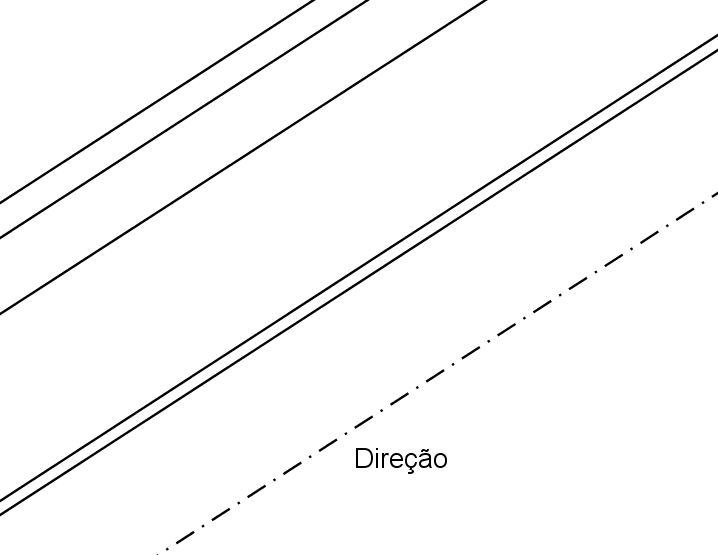
\includegraphics[width=\linewidth]{analitica/imagens/vetor1.png}
\caption{Direção}
\label{fig:direcao}
\end{minipage} \hfill
\begin{minipage}[b]{0.37\linewidth}
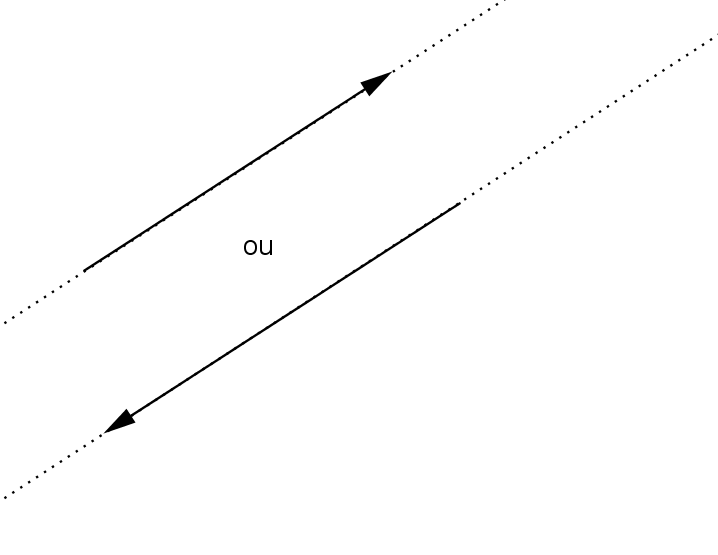
\includegraphics[width=\linewidth]{analitica/imagens/vetor2.png}
\caption{Sentido}
\label{fig:direc}
\end{minipage}
\end{figure}

Chamamos de \textbf{vetor} uma coleção de setas (ou flechas) que têm mesmo \textbf{comprimento} ou módulo, mesma \textbf{direção} e mesmo \textbf{sentido}. Cada seta é um representante do vetor. Assim, a ideia de vetor nos conduz a algo do tipo:

\begin{figure}[H]
\centering
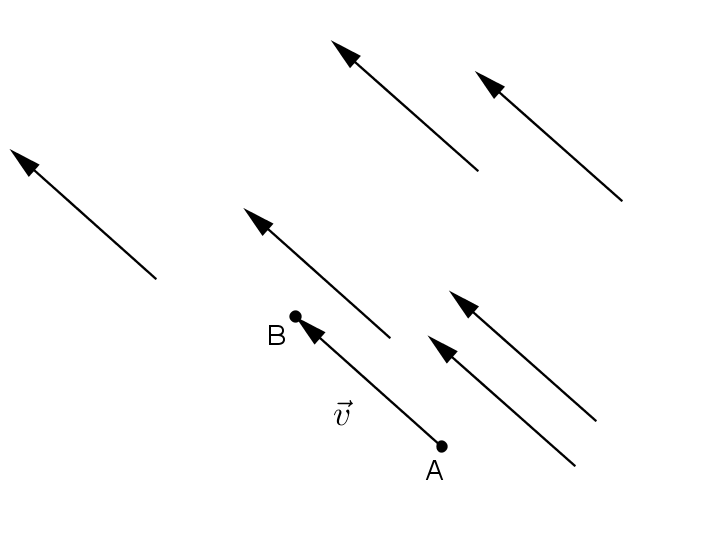
\includegraphics[scale=0.92]{analitica/imagens/vetor3.png}
\caption{Diversos representantes do mesmo vetor $\vec{v}$.}
\label{fig:vetor}
\end{figure}

\vspace{-0.4cm}
Quando escrevermos $\vec{v}=\overrightarrow{AB}$ significa que $\vec{v}$ é representado pela seta $\overrightarrow{AB}$. Porém, qualquer outra seta com o mesmo módulo (o módulo de $\vec v$ é indicado por $\Vert \vec v \Vert$), direção e sentido, representa também o mesmo vetor $\vec{v}$.

Dados os vetores $\vec{v}$ e $\vec{w}$ temos que:
\begin{enumerate}[i)]
\item o vetor de comprimento zero é chamado vetor nulo e denotado com $\overrightarrow{0}$;
\item o vetor $-\vec{v}$ é um vetor com o mesmo ``tamanho'' e mesma direção de $\vec{v}$ apenas com sentido oposto;
\item a soma dos vetores é obtida colocando a origem de $\vec{w}$ na extremidade de $\vec{v}$. O vetor soma tem origem no ponto inicial de $\vec{v}$ e extremidade no ponto final de $\vec{w}$;
 
\begin{figure}[H]
\centering
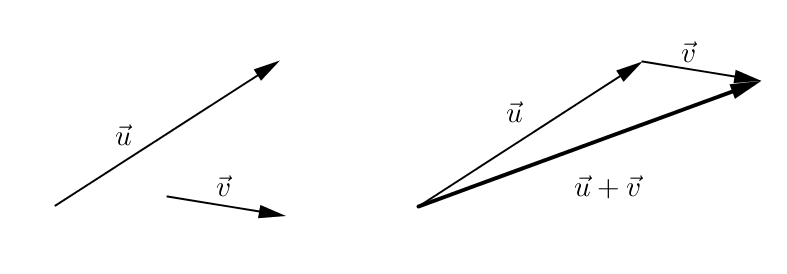
\includegraphics[scale=1.2]{analitica/imagens/vetor4.png}
\caption{Soma de dois vetores.}
\label{fig:somavetor}
\end{figure}

\vspace{-0.4cm}
\item se $k\in \mathbb{R}^{*}$ e $\vec{v}$ não é o vetor nulo, então $k\vec{v}$ é um vetor com a mesma direção de $\vec{v}$, comprimento igual a $|k|$ vezes o de $\vec{v}$, e sentido igual ao de $\vec{v}$ para $k>0$ e contrário ao de $\vec{v}$ para $k<0$.
\end{enumerate}

\subsection{Casos particulares de vetores}

Para a continuação do estudo, é preciso que identifiquemos situações específicas de vetores:
\begin{enumerate}[(1)]
 \item \textbf{paralelos} - Dois vetores $\vec u$ e $\vec v$ são \textit{paralelos}, e indica-se por $\vec u \parallel \vec v$, se os seus representantes tiverem a mesma direção.
 \item \textbf{iguais} - Dois vetores $\vec u$ e $\vec v$ são \textit{iguais}, e indica-se por $\vec u=\vec v$, se tiverem o mesmo módulo, mesma direção e mesmo sentido.
 \item \textbf{unitário} - É chamado de vetor \textit{unitário} aquele que tiver comprimento ou módulo igual a 1. Se $\Vert \vec v \Vert\neq 0$, o \textit{versor} de $\vec v$ é o vetor unitário com mesma direção e sentido de $\vec v$. Por exemplo, se $\Vert \vec v \Vert =3$, então o versor de $\vec v$ será $\frac{\vec v}{\Vert \vec v \Vert}=\frac{\vec v}{3}$.
 \item \textbf{oposto} - A cada vetor não-nulo $\vec v$ é associado um vetor \textit{oposto} $-\vec v$, que possui mesmo módulo e direção, mas sentido contrário de $\vec v$.
 \item \textbf{ortogonais} - Dois vetores $\vec u$ e $\vec v$ são \textit{ortogonais}, indicando-se $\vec u \perp \vec v$, se algum representante de $\vec u$ formar ângulo reto com algum representante de $\vec v$.
 \item \textbf{coplanares} - Dois ou mais vetores são \textit{coplanares} se existir algum plano onde estes vetores estão representados. Observe que \textit{dois vetores} são sempre coplanares, pois basta escolher um ponto $P$ e representar ambos a partir deste ponto. 
\end{enumerate}

\section{Abordagem algébrica: vetores no plano}

\begin{df}
Um vetor $\vec{v}$ é representado por diferentes setas no plano cartesiano.
\end{df}

\begin{figure}[H]
\centering
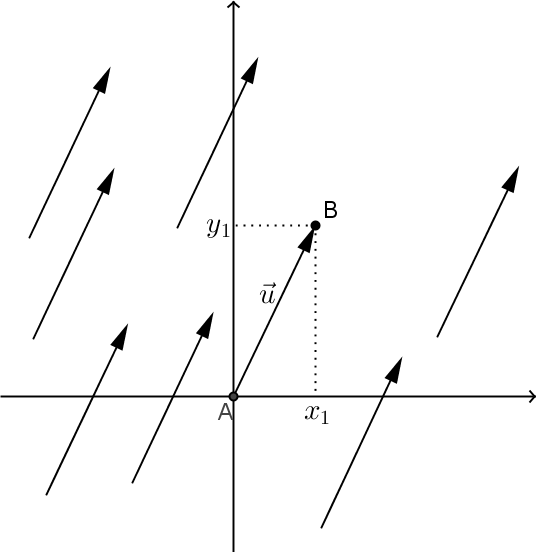
\includegraphics[scale=1.2]{analitica/imagens/vetor5.png}
\caption{Vetores no plano.}
\label{fig:vetorplano}
\end{figure}

Posicionando $\vec{v}$ com seu ponto inicial na origem do sistema, as coordenadas do ponto $B(x_1, y_1)$ (seu ponto final) são chamadas de componentes de $\vec{v}$ e escrevemos $\vec{v}=(x_1, y_1)$. A seta $\overrightarrow{AB}$ é chamada de representação posicional de $\vec{v}$.

\begin{exemplo} trace a representação posicional de $\vec{v}=(4, 2)$ e responda qual o:

\begin{figure}[H]
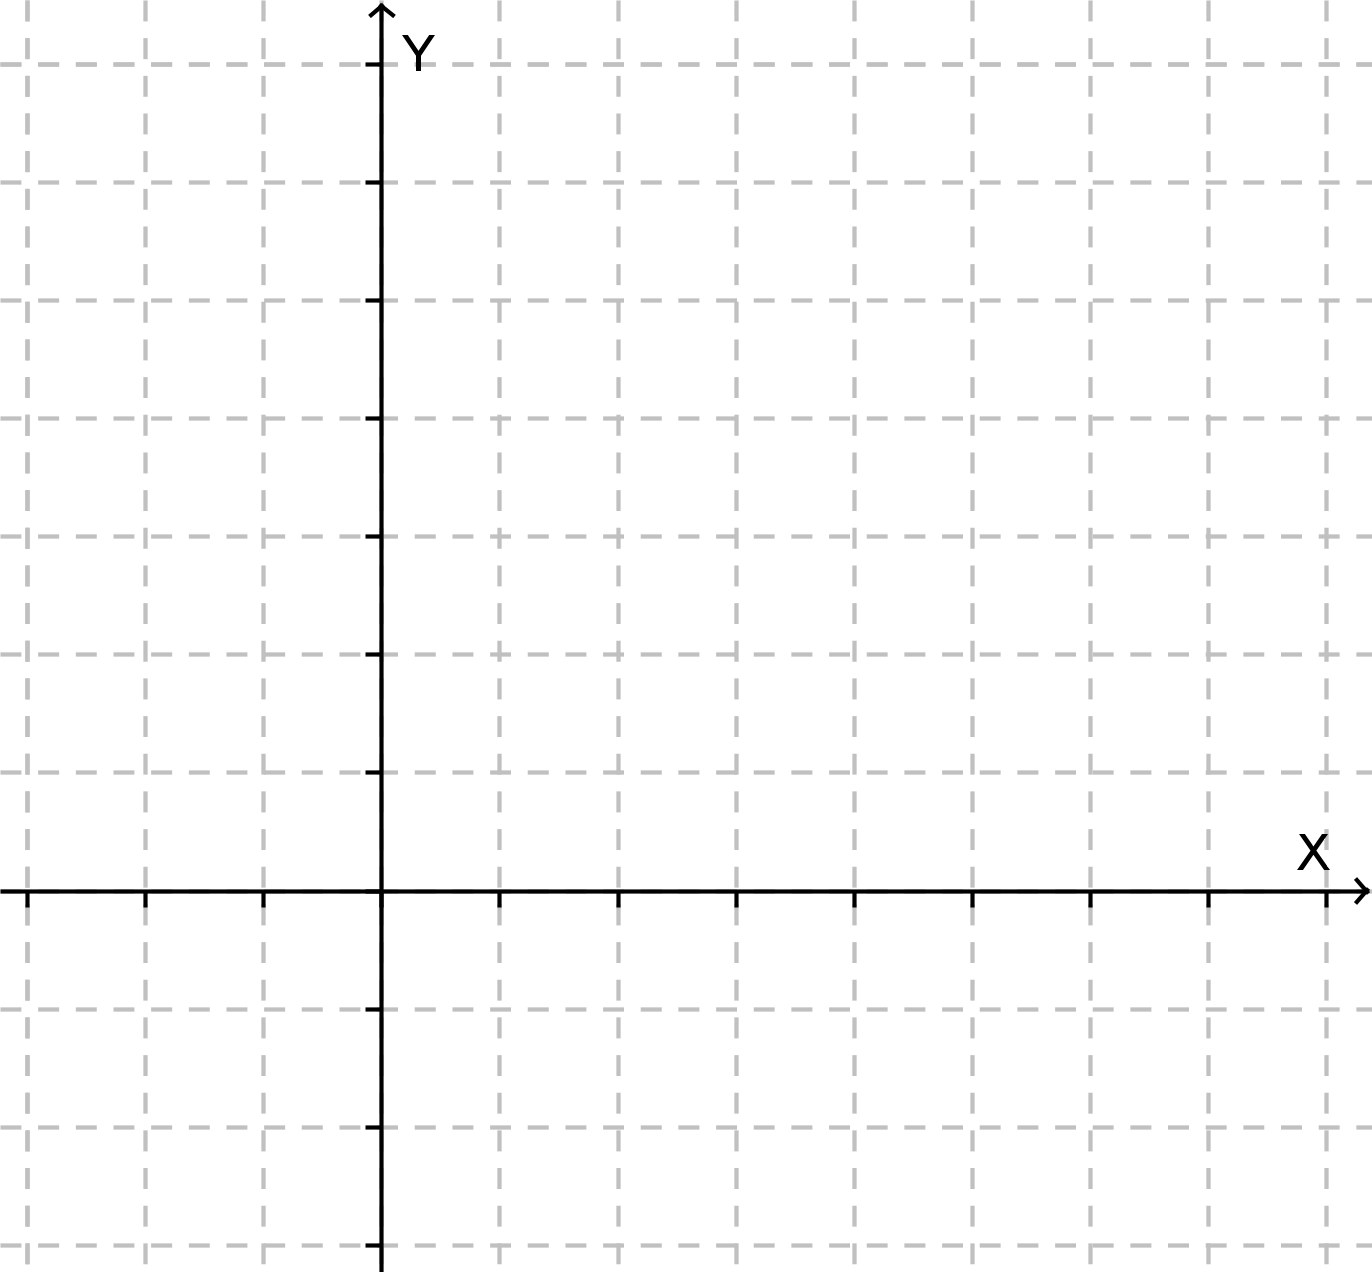
\includegraphics[scale=0.47]{analitica/imagens/malha.png}
\end{figure}

\begin{enumerate}[a)]
  \item ponto terminal de $\vec{v}$, se o ponto inicial for $(-2, 3)$.
  \item ponto inicial de $\vec{v}$, se o ponto terminal for $(6, 1)$.
\end{enumerate}
\end{exemplo}

\begin{df}
Os vetores $\vec{u}=(x_1, y_1)$ e $\vec{v}=(x_2, y_2)$ são iguais se e somente se $x_1=x_2$ e $y_1=y_2$.
\end{df}

\subsection{Operações com vetores}

Dados os vetores $\vec{u}=(x_1, y_1)$ e $\vec{v}=(x_2, y_2)$ temos que:

\begin{itemize}
\item $\vec{u}+\vec{v}=(x_1+x_2, y_1+y_2)$
\item $\vec{u}-\vec{v}=(x_1-x_2, y_1-y_2)$
\item $k\cdot \vec{u}=(k\cdot x_1, k\cdot y_1)$
\end{itemize}

\begin{exemplo} Sendo $\vec{u}=(3, 1)$ e $\vec{v}=(1, 2)$, determine o que é pedido:

\begin{figure}[H]
\begin{minipage}[b]{0.3\linewidth}
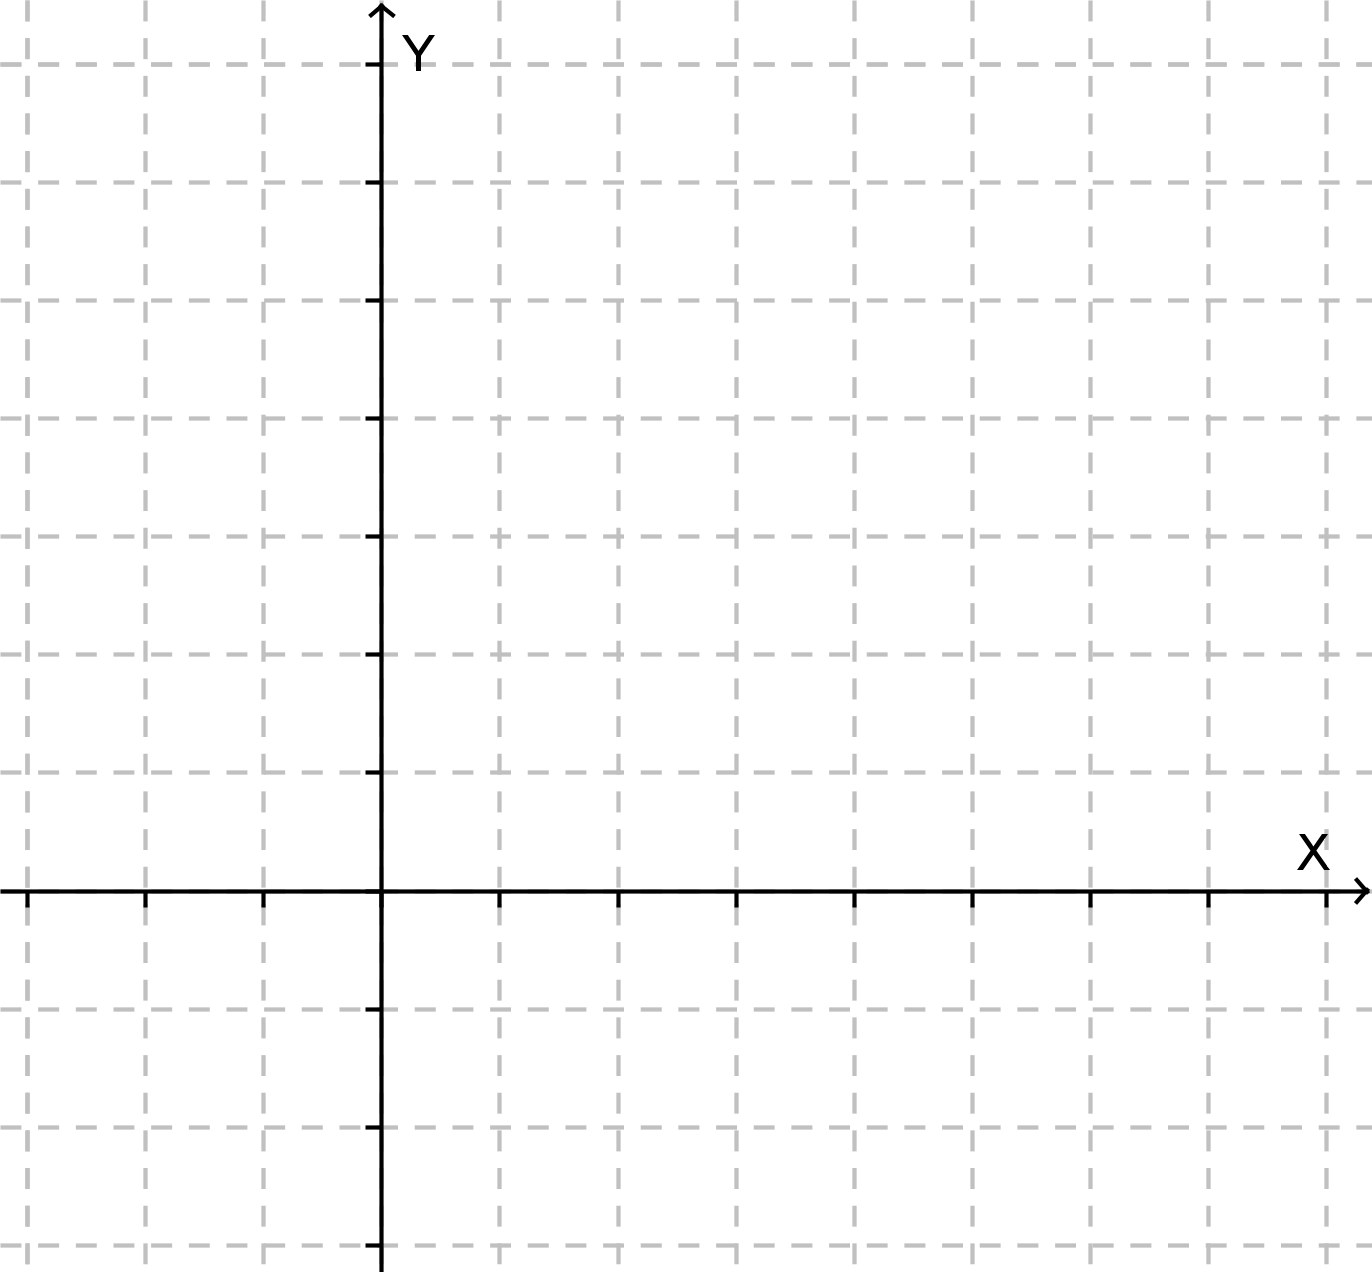
\includegraphics[width=\linewidth]{analitica/imagens/malha.png}
\caption{a) $\vec{u}+\vec{v}=$}
\end{minipage} \hfill
\begin{minipage}[b]{0.3\linewidth}
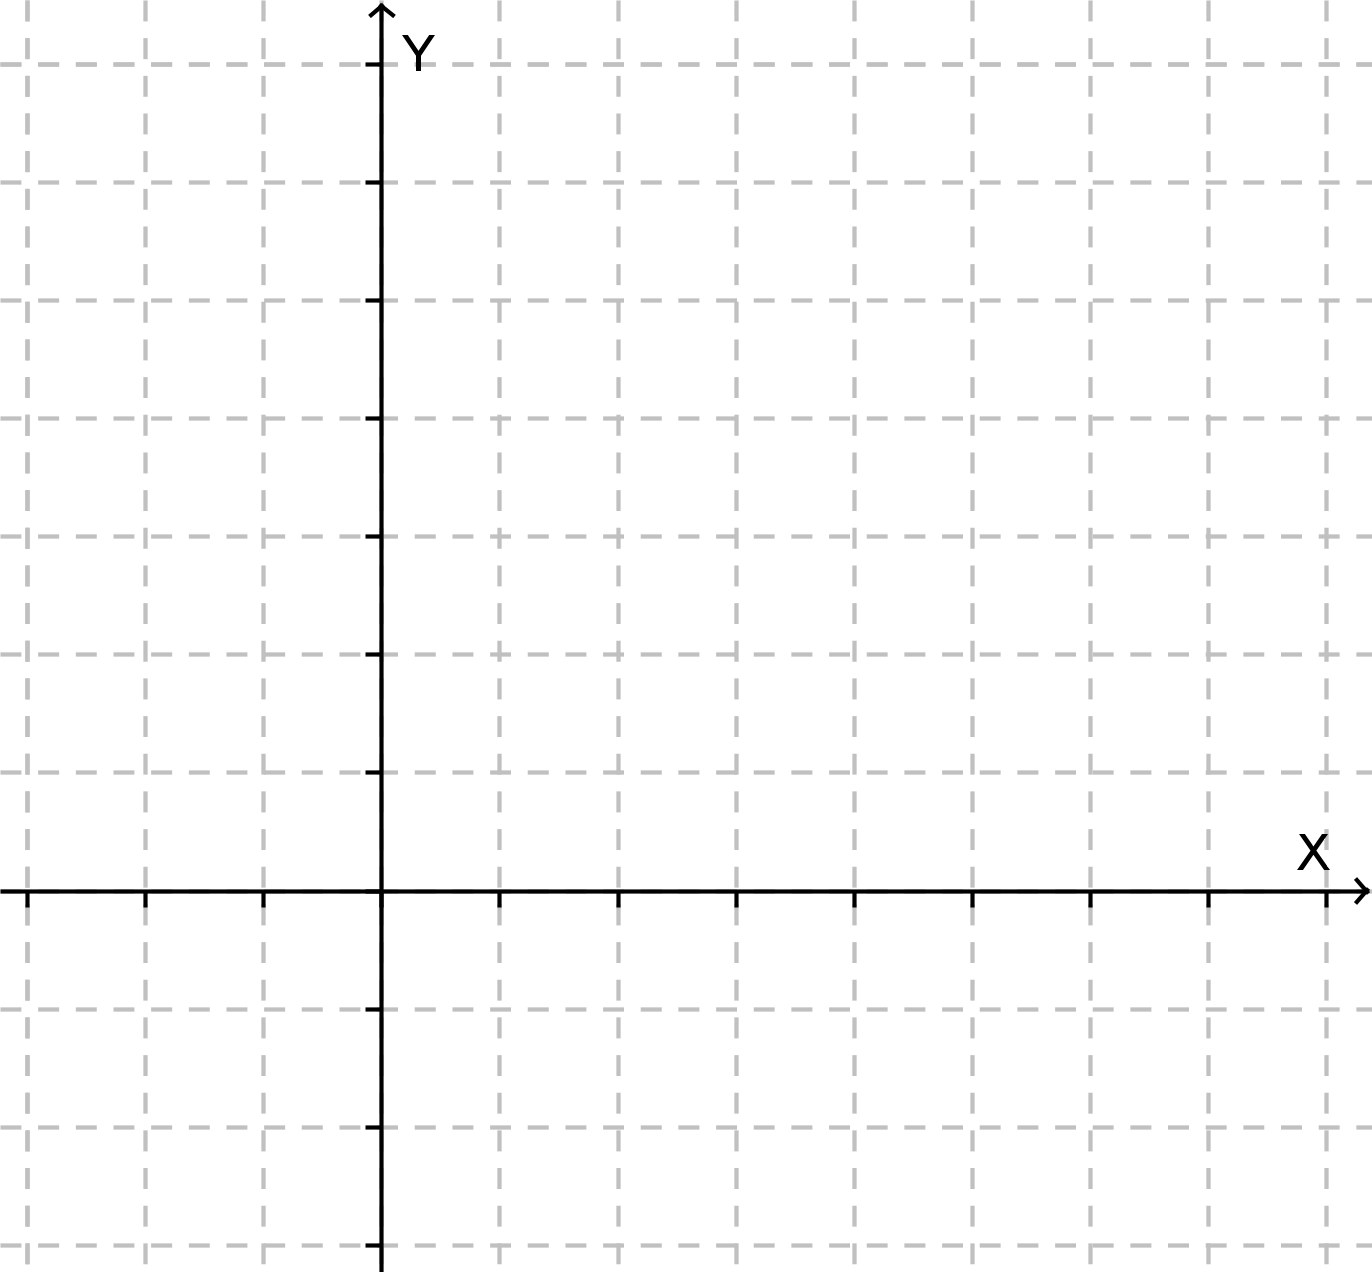
\includegraphics[width=\linewidth]{analitica/imagens/malha.png}
\caption{b) $\vec{u}-\vec{v}=$}
\end{minipage}\hfill
\begin{minipage}[b]{0.3\linewidth}
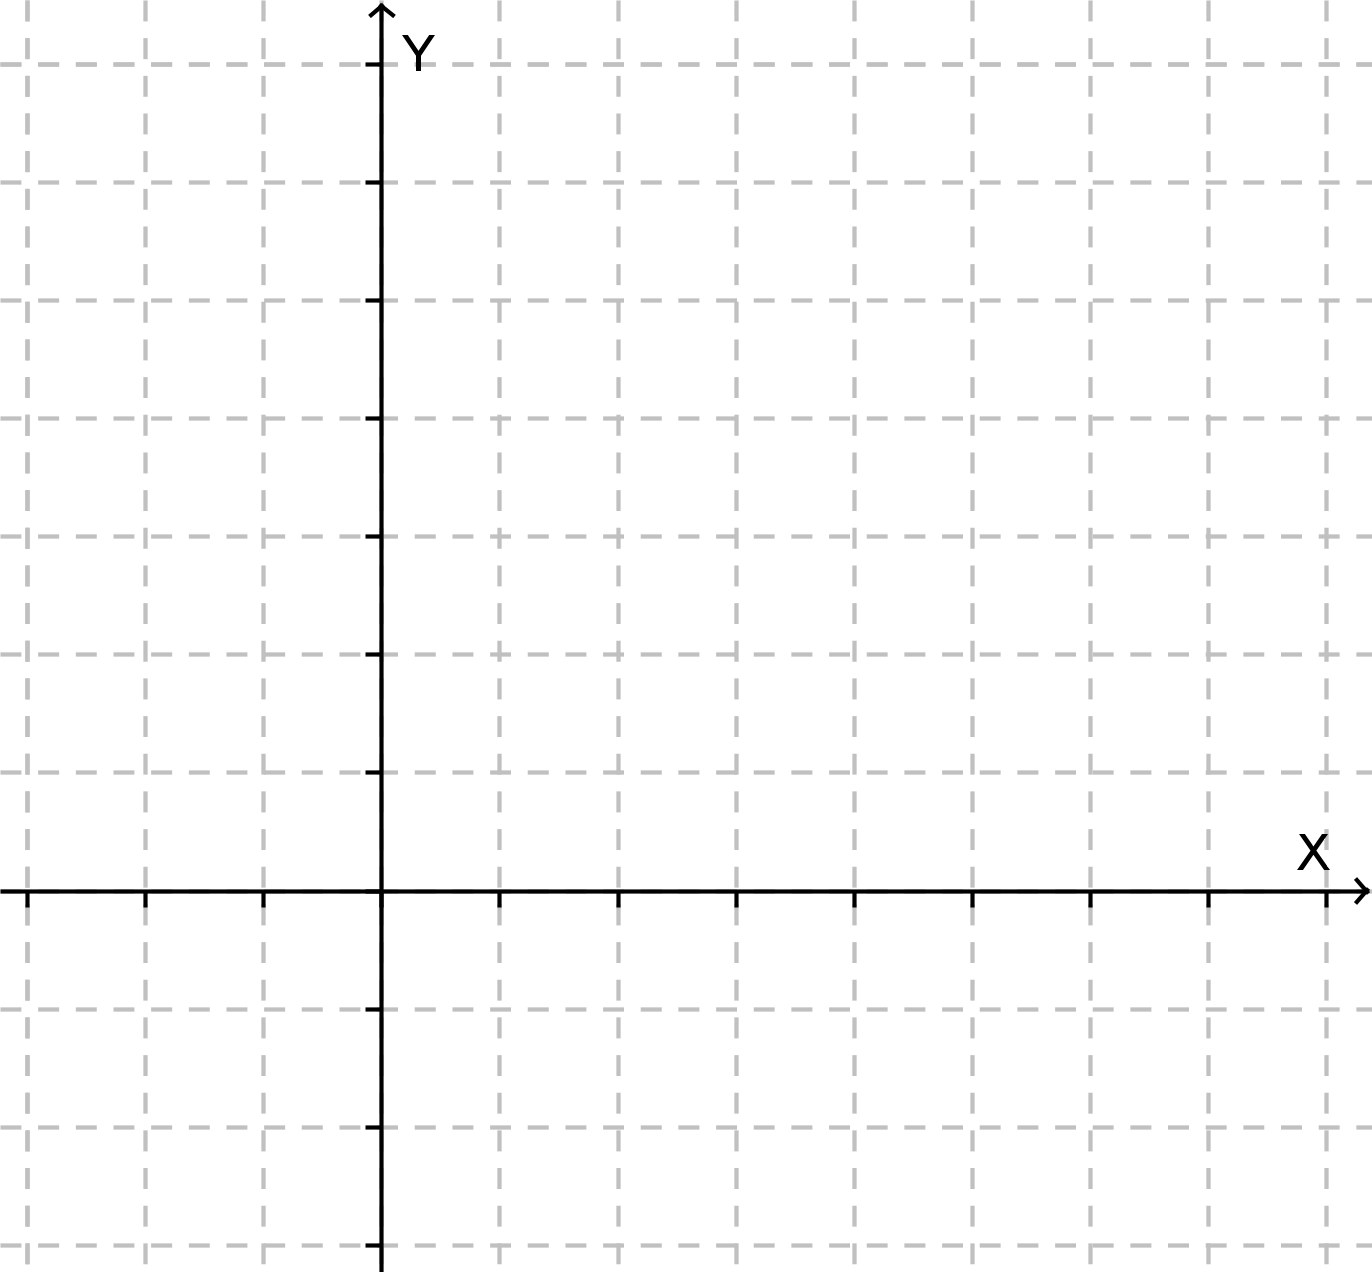
\includegraphics[width=\linewidth]{analitica/imagens/malha.png}
\caption{c) $3\cdot \vec{v}=$}
\end{minipage}
\end{figure}

d) $a$ e $b$ sabendo que $a\cdot \vec{u}+b\cdot \vec{v}=(9, 8)$.
\end{exemplo}
\vspace{2cm}

\subsection{Expressão analítica de um vetor}

Consideremos agora o vetor $\vec{i}=(1,0)$ e $\vec{j}=(0,1)$. Será que poderemos dizer que o vetor $\vec{v}=(2,3)$, por exemplo, pode ser escrito como $\vec{v}=2\vec{i}+3\vec{j}$? Verifique graficamente.

É fácil ver que esse fato ocorre para todo vetor do plano. Mais tarde estudaremos que esses vetores $\vec{i}$ e $\vec{j}$ formam uma base do $\mathbb{R}^2$. Isto é, dado um vetor $\vec{v}$, existe um único par de números reais, $x$ e $y$, tais que $\vec{v}=x\vec{i}+y\vec{j}$.

\begin{figure}[H]
\centering
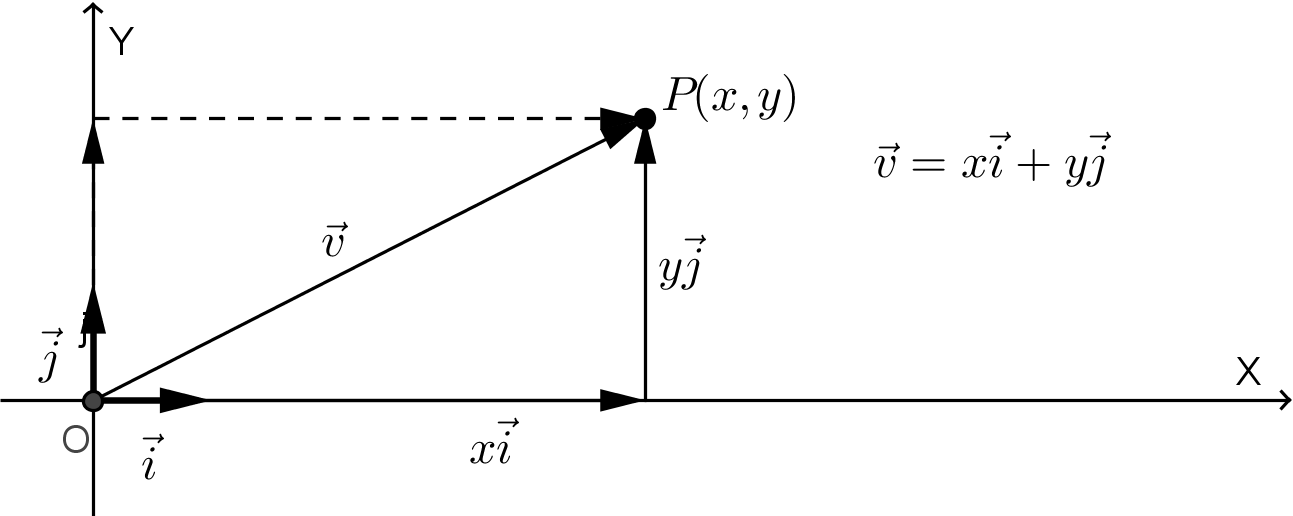
\includegraphics[scale=0.82]{analitica/imagens/combinalinear.png}
\end{figure}

\subsection{Vetor definido por dois pontos}

Muitas vezes um vetor é representado por uma seta que não parte da origem do sistema. Sendo $\vec{v}=\overrightarrow{AB}$, com $A(x_a, y_a)$ e $B(x_b, y_b)$, como podemos determinar as componentes de $\vec{v}$?

\begin{multicols}{2}
\begin{figure}[H]
\centering
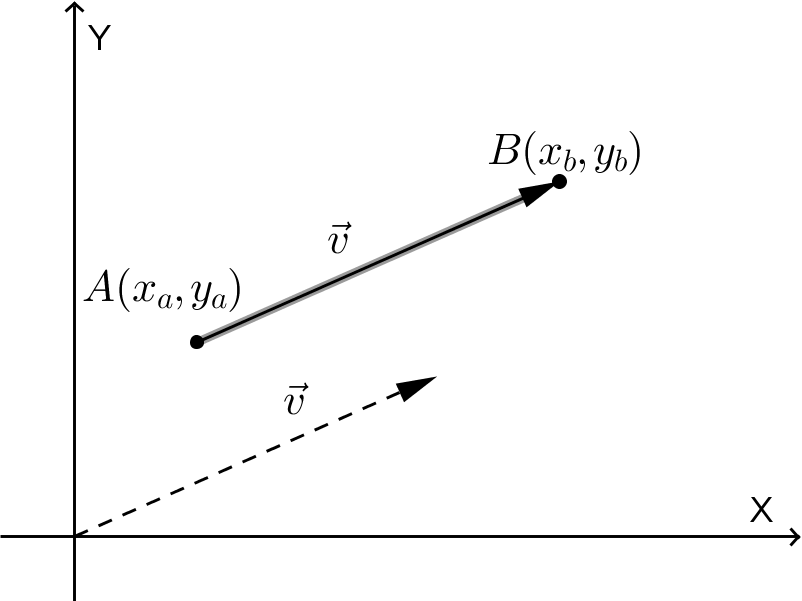
\includegraphics[scale=0.87]{analitica/imagens/doispontos.png}
\end{figure}

$$\vec{v}=\overrightarrow{AB}=\ldots$$
\end{multicols}


\begin{exemplo} sendo $A(1, 2)$, $B(7, 3)$ e $C(5, 7)$, determine os vetores:
\begin{enumerate}[a)]
 \item $\overrightarrow{AB}$
 \item $\overrightarrow{CB}$
 \item $\overrightarrow{AC}$
\end{enumerate}
\end{exemplo}

\subsection{Paralelismo de vetores}

Se dois vetores $\vec{u}$ e $\vec{v}$ são paralelos, então existe um número $\alpha$ tal que $\vec{u}=\alpha \vec{v}$.

Se $\vec{u}=(x_1, y_1)$ e $\vec{v}=(x_2, y_2)$ então $(x_1, y_1)=\alpha(x_2, y_2)$ e portanto $x_1=\alpha x_2$ e $y_1=\alpha y_2$ de onde se conclui que $\displaystyle \alpha=\frac{x_1}{x_2}=\frac{y_1}{y_2}$. Logo

$$\vec{u} \parallel \vec{v}  \qquad \Longleftrightarrow \qquad \frac{x_1}{x_2}=\frac{y_1}{y_2}$$

Observações:
\begin{enumerate}[a)]
 \item o vetor nulo $\vec{0}=(0, 0)$ é paralelo a qualquer vetor.
 \item se uma das componentes do vetor $\vec{v}$ é nula, a componente correspondente de qualquer vetor paralelo a $\vec{v}$ também é nula.
\end{enumerate}

\subsection{Módulo ou norma de um vetor}

A distância entre os pontos inicial e final do segmento orientado que representa um vetor $\vec{v}$ é chamada de módulo de \textit{módulo} ou \textit{norma} de $\vec{v}$ e denotada por $\Vert\vec{v}\Vert$. 

Essa distância não muda se o vetor for transladado, logo, para propósitos  de  cálculo  da  norma, podemos supor que o vetor está posicionado com seu ponto inicial na origem.

\begin{figure}[H]
\centering
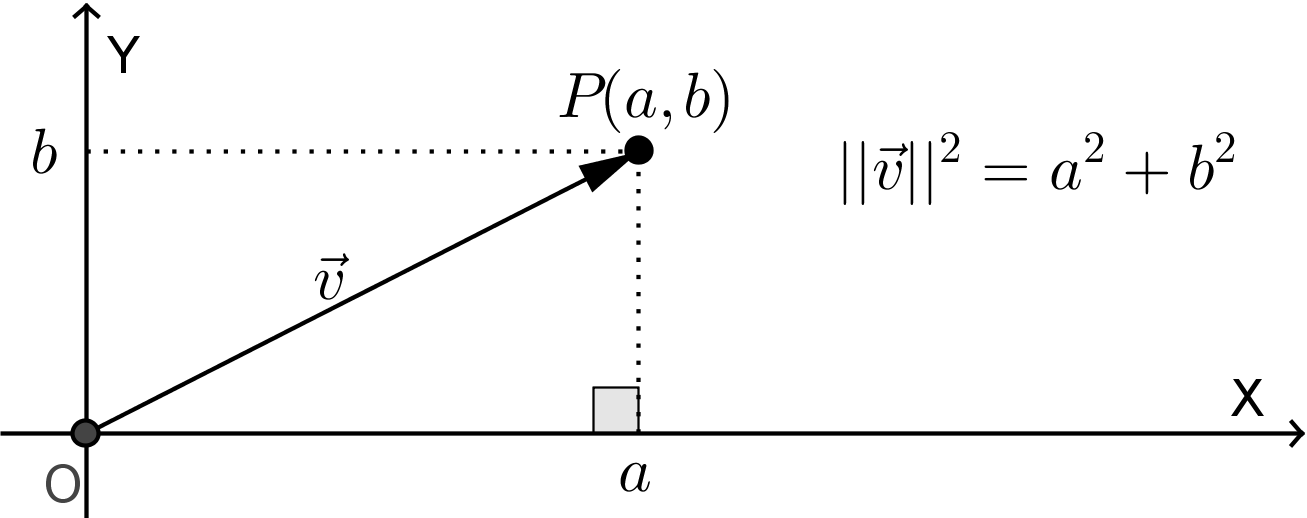
\includegraphics[scale=0.8]{analitica/imagens/norma.png}
\end{figure}

Pelo teorema de Pitágoras temos que a norma do vetor $\vec{v}=(a)$ é dada por: $$\Vert\vec{v}\Vert=\sqrt{a^2+b^2}$$

\begin{exemplo} sendo $\vec{v}=(4, 2)$, determine:

\begin{enumerate}[a)]
 \item o módulo de $\vec{v}$. \vspace{1cm}
 \item um vetor unitário com mesma direção e sentido de $\vec{v}$. \vspace{1cm}
 \item um vetor unitário com mesma direção e sentido contrário de $\vec{v}$. \vspace{2cm}
\end{enumerate}
\end{exemplo}

\section{Abordagem algébrica: vetores no espaço}

Como os elementos do $\mathbb{R}^2$ e $\mathbb{R}^3$ são representados, respectivamente, por pares $(x,y)$ e ternas $(x,y,z)$, estes elementos podem ser interpretados como pontos ou vetores. Então, $(x,y)$ e $(x,y,z)$ são as coordenadas de um ponto que marca uma posição ou de um vetor que define um deslocamento.

No espaço, como todo elemento do $\mathbb{R}^3$, os vetores serão representados por três componentes: $$\vec v=(a,b,c)$$

\begin{figure}[H]
\centering
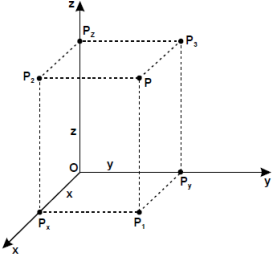
\includegraphics[scale=0.7]{analitica/imagens/vetor-r3-3.png}
\end{figure}

No plano, os vetores $\vec i=(1,0)$ e $\vec j=(0,1)$ formam uma base do $\mathbb{R}^2$, e com isso um vetor $\vec v=(a,b)$ pode ser escrito como $\vec v=a\vec i+b\vec j$.

No espaço, os vetores $\vec i=(1,0,0)$, $\vec j=(0,1,0)$ e $\vec k=(0,0,1)$ formam uma base do $\mathbb{R}^3$, e com isso um vetor $\vec v=(a,b,c)$ pode ser escrito como $\vec v=a\vec i+b\vec j+c\vec k$.

As relações algébricas para o espaço, são análogas ao do plano, pois basta acrescentar uma componente na representação:
\begin{enumerate}[I)]
 \item Dois vetores $\vec u=(x_1, y_1, z_1)$ e $\vec v=(x_2, y_2, z_2)$ são \textbf{iguais} se, e somente se, $x_1=x_2$, $y_1=y_2$ e $z_1=z_2$.
 \item Dados os vetores $\vec u=(x_1, y_1, z_1)$ e $\vec v=(x_2, y_2, z_2)$ e $\alpha \in \mathbb{R}^2$, define-se:
   \begin{enumerate}
     \item $\vec u +\vec v=(x_1+x_2, y_1+y_2, z_1+z_2)$
     \item $\alpha \vec u=(\alpha x_1, \alpha y_1, \alpha z_1)$
   \end{enumerate}
 \item Se $A=(x_1, y_1, z_1)$ e $B=(x_2, y_2, z_2)$ são \textbf{dois pontos} quaisquer do espaço, então $\overrightarrow{AB}=B-A=(x_2-x_1, y_2-y_1, z_2-z_1)$. E se $\vec v=\overrightarrow{AB}=B-A$, então $$B=A+\vec v$$
 \item Se os vetores $\vec u=(x_1, y_1, z_1)$ e $\vec v=(x_2, y_2, z_2)$ são \textbf{paralelos}, então $\vec u=\alpha \vec v$ ou $$\frac{x_1}{x_2}=\frac{y_1}{y_2}=\frac{z_1}{z_2}$$

Observações:
 \begin{enumerate}[a)]
  \item o vetor nulo $\vec{0}=(0, 0, 0)$ é paralelo a qualquer vetor.
  \item se uma das componentes do vetor $\vec{v}$ é nula, a componente correspondente de qualquer vetor paralelo a $\vec{v}$ também é nula.
 \end{enumerate}
 
 \item O \textbf{comprimento} (norma ou módulo) do vetor $\vec v=(a, b, c)$ é dado por $$\Vert \vec v \Vert=\sqrt{a^2+b^2+c^2}$$

\end{enumerate}

\section{Combinação linear de vetores}

Sejam os vetores $\vec v_1, \vec v_2, \vec v_3, \ldots, \vec v_n $. Um vetor $v$ é combinação linear (CL) dos vetores $\vec v_1, \vec v_2, \vec v_3, \ldots, \vec v_n $ se existirem as constantes $a_1, a_2, a_3, \ldots, a_n \in \mathbb{R}$, tais que $$\vec v=a_1\vec v_1+a_2\vec v_2+a_3\vec v_3+\ldots+a_n\vec v_n$$

Nem sempre é possível expressar um dado vetor como combinação linear de outros dois e, quando possível, pode existir mais de uma solução. Para entender esta afirmação, repare que este problema é equivalente a achar a solução de um sistema de equações lineares. O número de componentes do vetor fornece o número de equações do sistema. Se o sistema for determinado será possível resolver o problema dado.
\chapter{Produto Escalar}

\begin{df} Chama-se produto escalar (ou produto interno usual) de dois vetores $\vec u$ e $\vec v$ o número real representado por $\vec u \cdot \vec v$ ou $<\vec u, \vec v>$ e calculado pela soma dos produtos das componentes correspondentes dos vetores.

No plano, $\mathbb{R}^2$, se $\vec u=(x_1, y_1)$ e $\vec v=(x_2, y_2)$ então $\vec u \cdot \vec v = x_1\cdot x_2 + y_1\cdot y_2$.

No espaço, $\mathbb{R}^3$, se $\vec u=(x_1, y_1, z_1)$ e $\vec v=(x_2, y_2, z_2)$ então $\vec u \cdot \vec v = x_1\cdot x_2 + y_1\cdot y_2+z_1\cdot z_2$.
\end{df}


\section{Propriedades do produto escalar}

\begin{enumerate}[(1)]
\item $\vec u\cdot \vec v=\vec v\cdot \vec u$
\item $\vec u\cdot (\vec v+\vec w)=\vec u\cdot \vec v+\vec u\cdot \vec w$
\item $\alpha(\vec u\cdot \vec v)=(\alpha \vec u)\cdot \vec v=\vec u\cdot (\alpha \vec v)$, com $\alpha \in \mathbb{R}$.
\item $\vec u\cdot \vec u=\Vert \vec u \Vert^2$
\item $\Vert \vec u\cdot \vec v\Vert \leq \Vert \vec u \Vert \Vert \vec v \Vert$ (Desigualdade de Schwarz)
\item $\Vert \vec u + \vec v\Vert \leq \Vert \vec u \Vert+ \Vert \vec v \Vert$ (Desigualdade Triangular)
\end{enumerate}

\subsection{Ângulo entre dois vetores}

Note que quando realizamos o produto escalar entre dois vetores, obtemos um número e que a definição na sua primeira forma nos dá informação sobre o ângulo entre os dois vetores, pois $$\cos{\theta}=\frac{\vec{u} \cdot \vec{v}}{\Vert\vec{u}\Vert \cdot \Vert\vec{v}\Vert}$$

\noindent onde $\theta$ é o ângulo entre os vetores com $0\leq \theta \leq \pi$. A demonstração deste fato pode ser obtida com a utilização da lei dos cossenos e de algumas propriedades (veja bibliografia específica indica.)

Com isso obtemos outra maneira de definir o produto escalar: $$\vec u \cdot \vec v=\Vert \vec u \Vert \cdot \Vert \vec v \Vert \cdot \cos{\theta}$$

Observação: da fórmula acima podemos ver que o sinal de $\vec{u} \cdot \vec{v}$ é o mesmo que o sinal de $\cos{\theta}$ e a partir daí, concluir se o ângulo entre os dois vetores é agudo, obtuso ou reto (vetores ortogonais).

\begin{figure}[H]
\begin{minipage}[b]{0.3\linewidth}
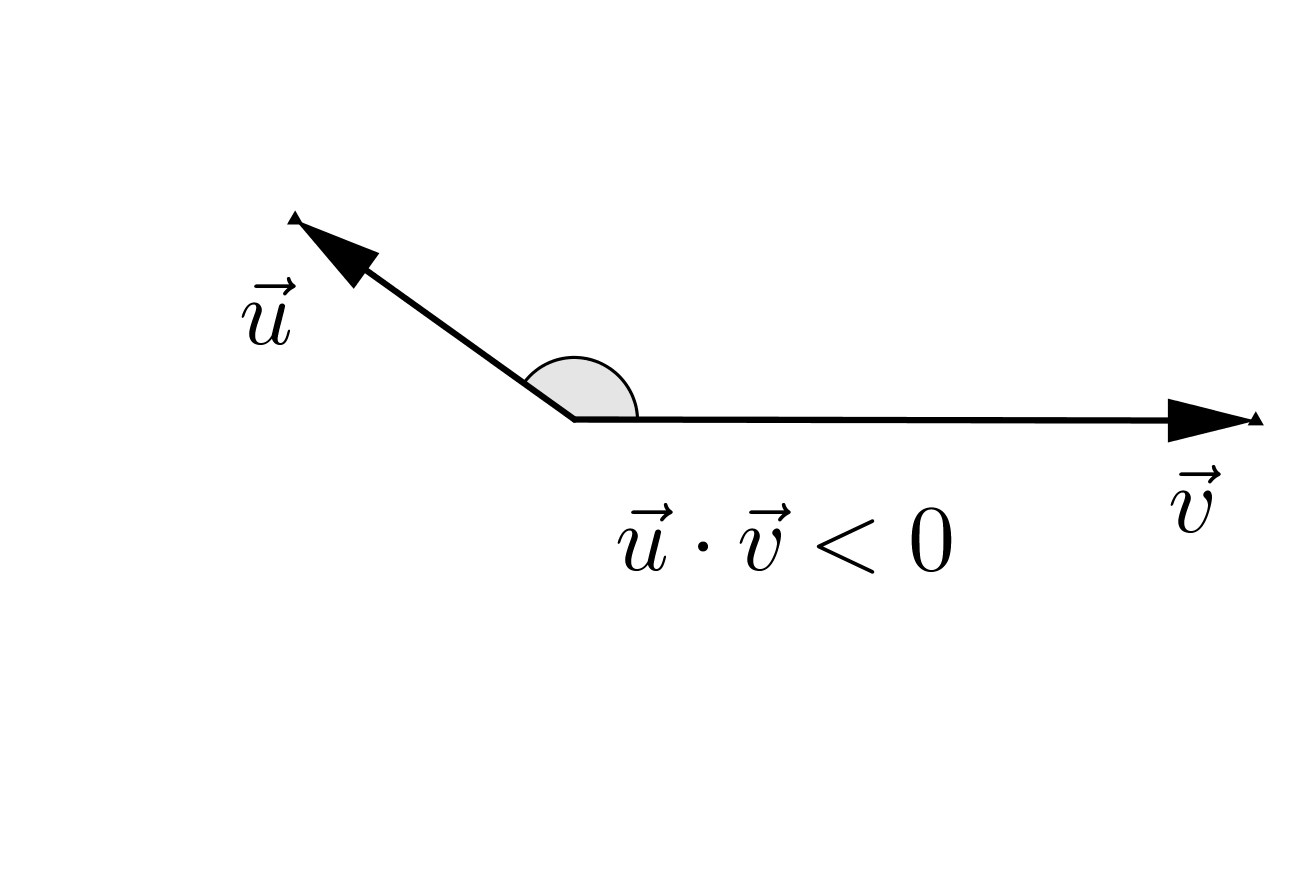
\includegraphics[width=\linewidth]{analitica/imagens/angvetores1.png}
\caption{Ângulo obtuso}
\end{minipage} \hfill
\begin{minipage}[b]{0.3\linewidth}
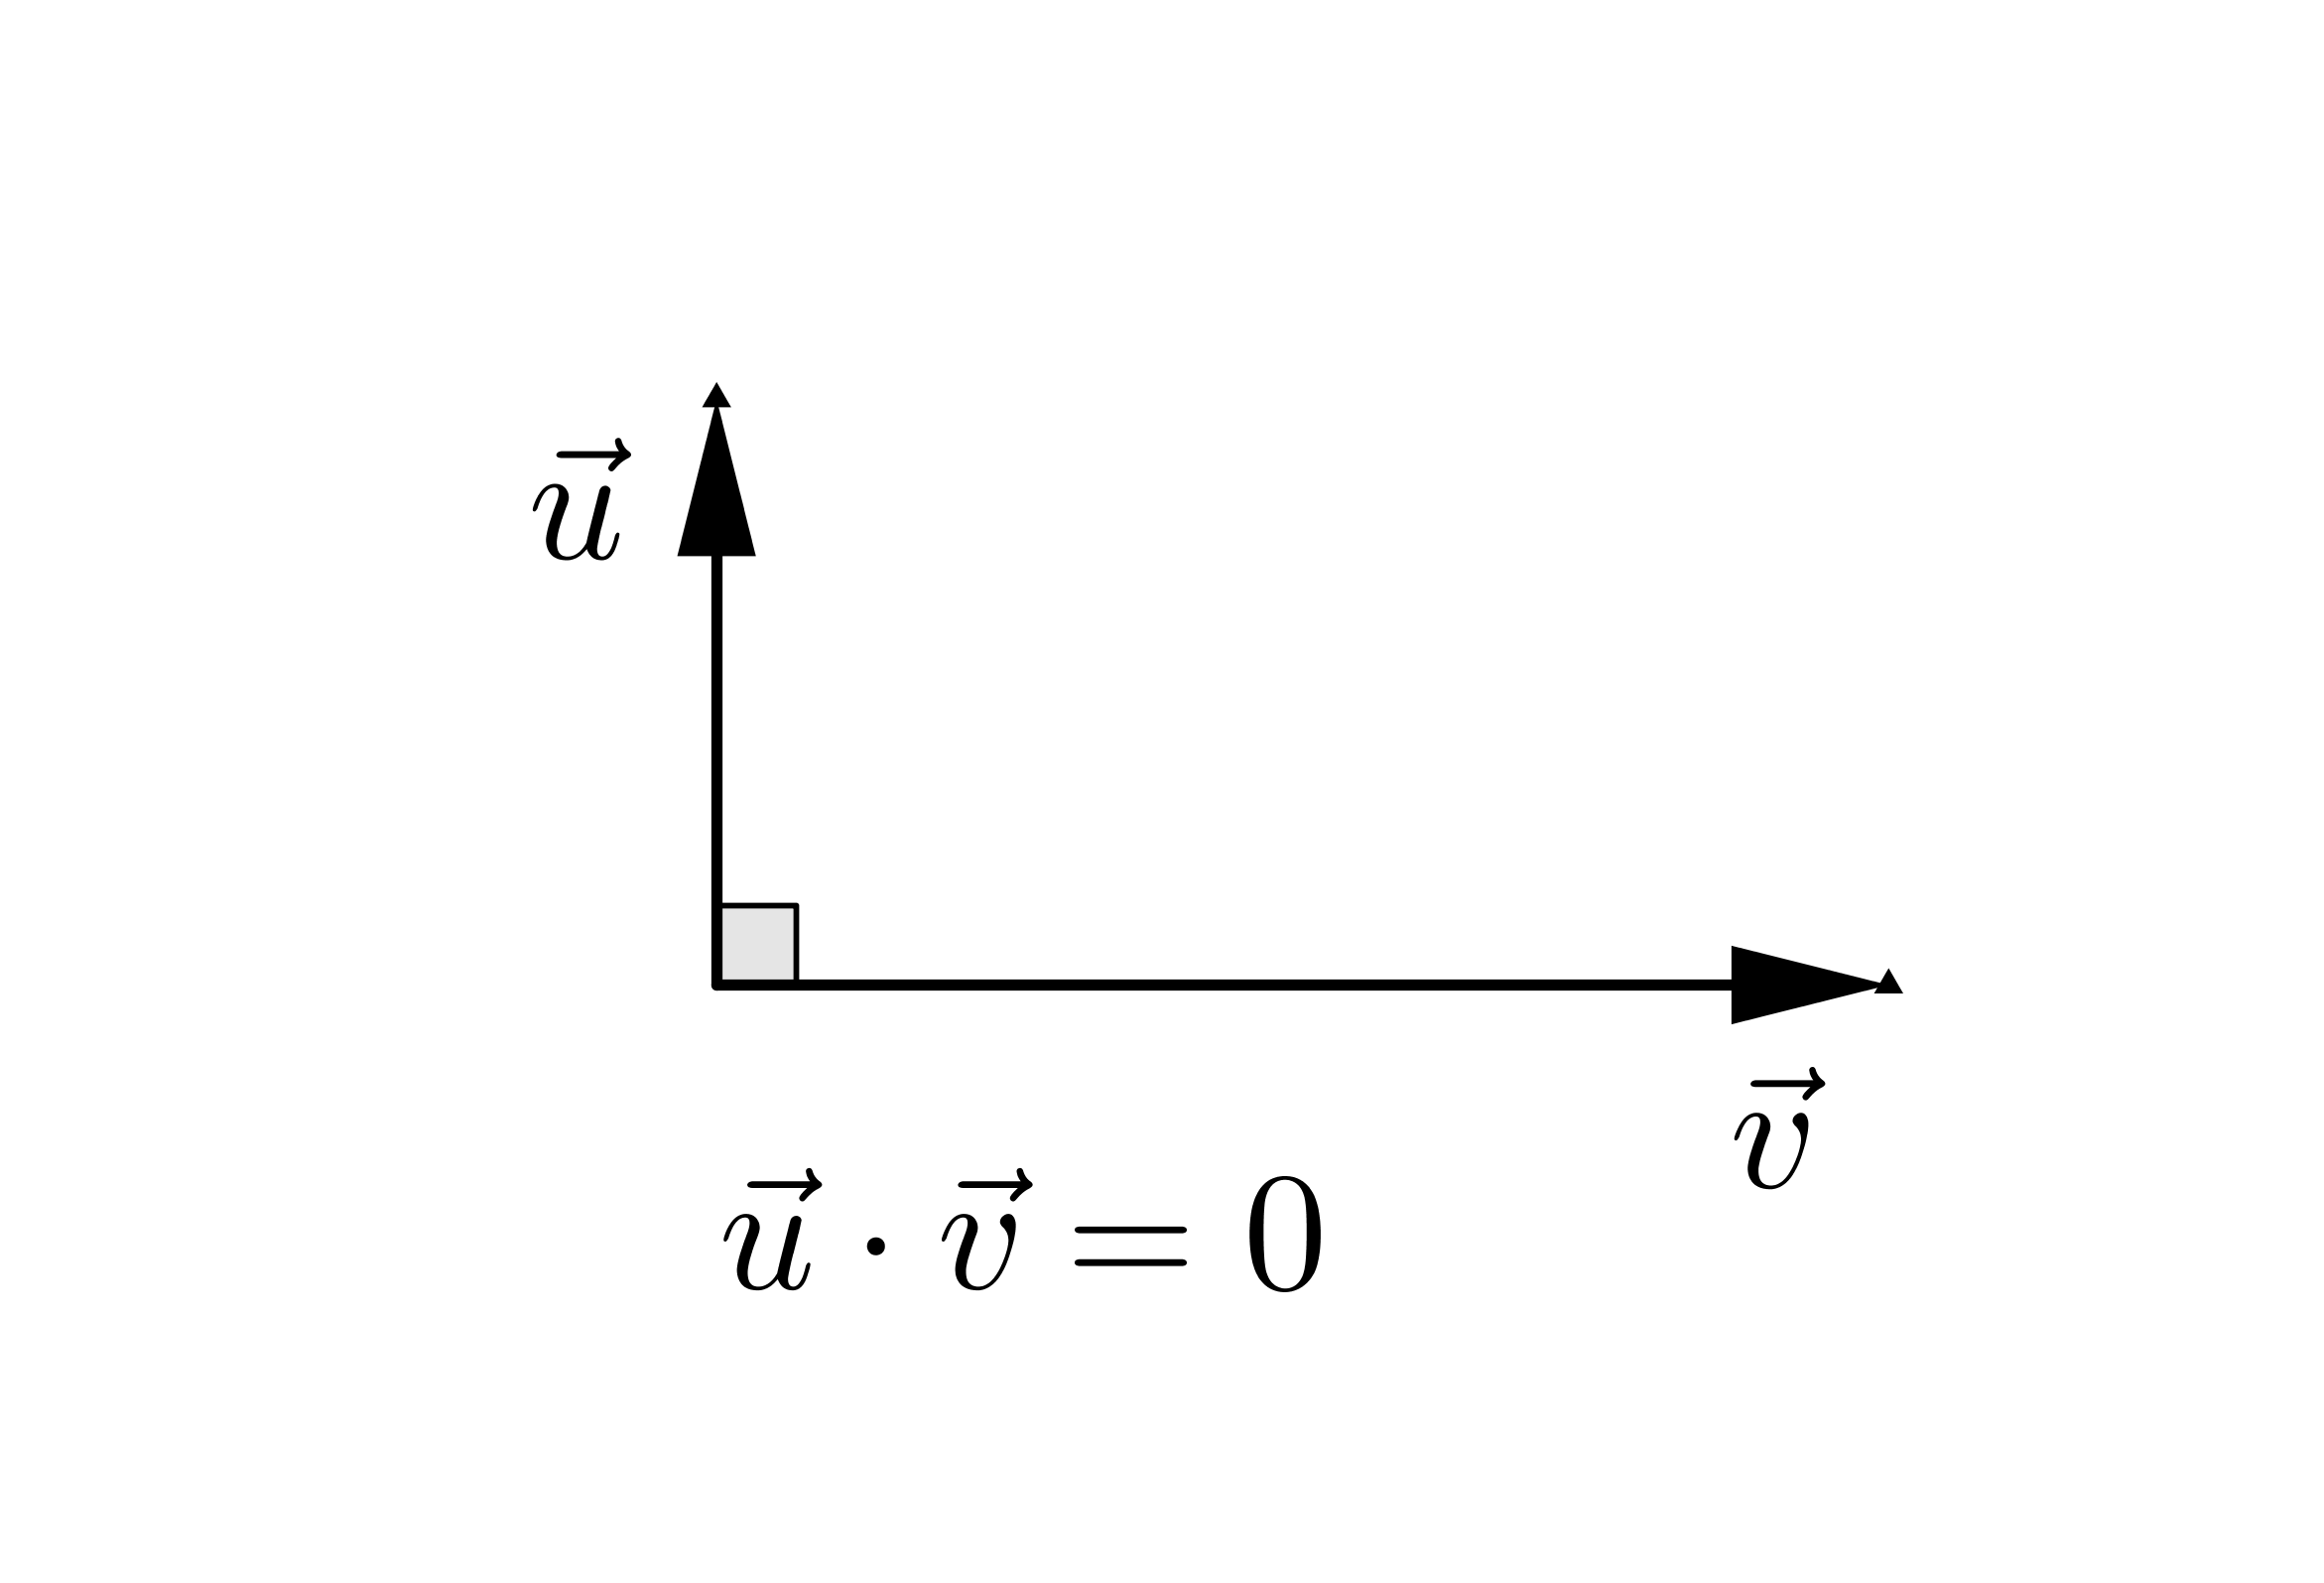
\includegraphics[width=\linewidth]{analitica/imagens/angvetores2.png}
\caption{Ângulo reto}
\end{minipage}\hfill
\begin{minipage}[b]{0.3\linewidth}
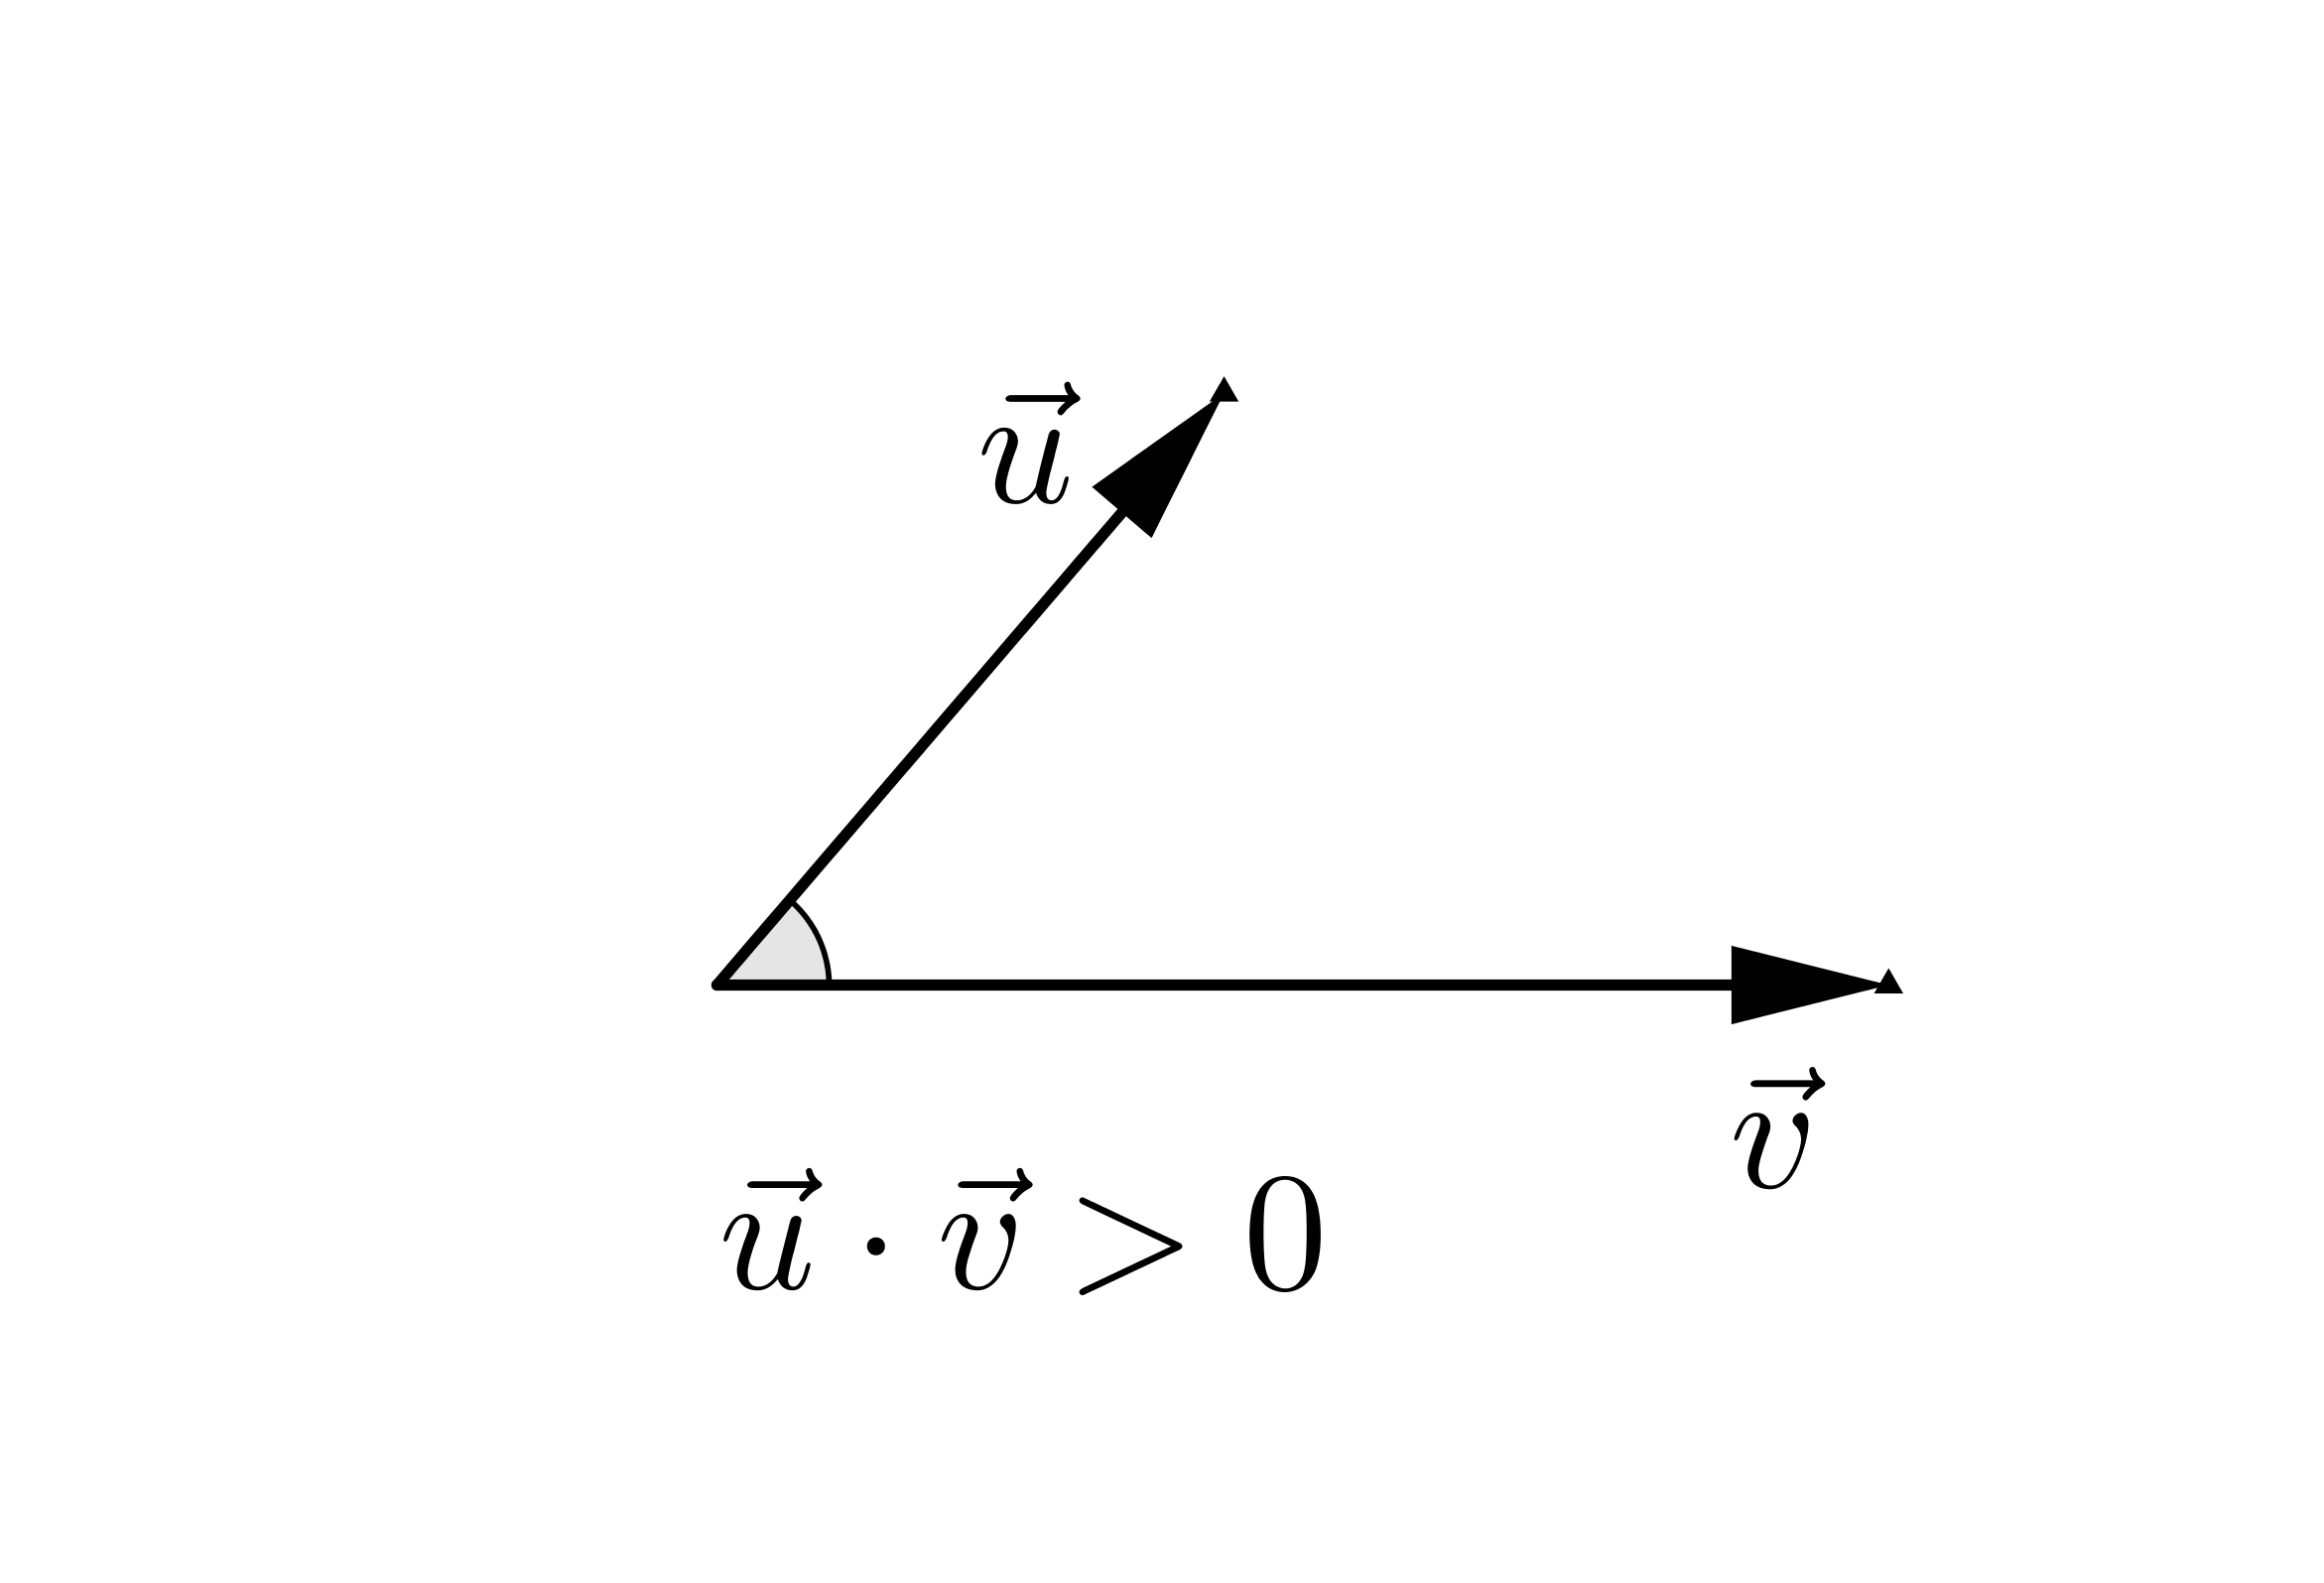
\includegraphics[width=\linewidth]{analitica/imagens/angvetores3.png}
\caption{Ângulo agudo}
\end{minipage}
\end{figure}

\begin{exemplo} dados os vetores $\vec{u}= (4, 3)$ e $\vec{v}=(2,-2)$, determine o cosseno do ângulo formado pelos vetores $\vec{u}$ e $\vec{v}$.
\end{exemplo}

\vspace{2cm}

\begin{exemplo} Qual o ângulo entre os vetores $\vec{u}=(1,-2, 3)$ e $\vec{v}=(4,5,2)$?
\end{exemplo}

\vspace{2cm}

\subsection{Projeção de um vetor sobre outro}

Sejam os vetores $\vec u$ e $\vec v$, pretendemos decompor um dos vetores, digamos $\vec v$, tal que $$\vec v=\vec v_1+\vec v_2$$ sendo $\vec v_1\parallel\vec u$ e $\vec v_2 \perp \vec u$.

\begin{figure}[H]
\centering
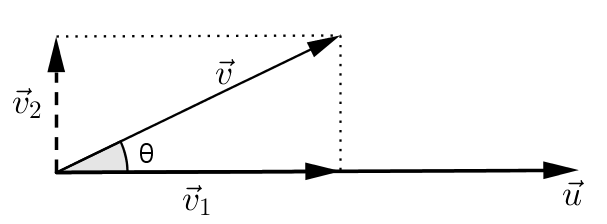
\includegraphics[scale=1]{analitica/imagens/projecao.png}
\end{figure}

O vetor $\vec v_1$ é chamado \textit{projeção ortogonal} de $\vec v$ sobre $\vec u$ e indicado por $$\vec v_1=proj_{\vec u}\vec v$$

\textbf{Demonstração:} Sendo $\vec v_1\parallel \vec u$, temos $\vec v_1=\alpha \vec u$, e como $\vec v_2=\vec v-\vec v_1=\vec v-\alpha\vec u$ é ortogonal a $\vec u$, temos\footnote{Observe que $\alpha$ é uma constante, já que o resultado do produto escalar é um número real.}

\begin{eqnarray*}
(\vec v-\alpha \vec u) \cdot \vec u & = & 0 \\
\vec v \cdot \vec u-\alpha \vec u \cdot \vec u& = &  0\\
\alpha \vec u \cdot \vec u& = &  \vec v \cdot \vec u\\
\alpha & = & \frac{\vec v \cdot \vec u}{\vec u \cdot \vec u}
\end{eqnarray*}

Lembrando que $\vec v_1=\alpha \vec u$, concluímos que  $\vec v_1= \left(\frac{\vec v \cdot \vec u}{\vec u \cdot \vec u}\right) \vec u$.

Portanto, a \textit{projeção ortogonal} de $\vec v$ sobre $\vec u$ é dada por $$proj_{\vec u}\vec v=\left(\frac{\vec v \cdot \vec u}{\vec u \cdot \vec u}\right) \vec u$$
\chapter{Produto vetorial}

O produto vetorial de dois vetores $\vec{u}\times \vec{v}$ apresenta como resultado um vetor, ao contrário do que acontece com o produto escalar $\vec{u}\cdot \vec{v}$ que resulta em um escalar (número real).

\begin{df} Dados os vetores $\vec{u}=(x_1, y_1, z_1)$ e $\vec{v}=(x_2, y_2, z_2)$, chama-se produto vetorial de $\vec{u}$ por $\vec{v}$, nesta ordem, ao vetor representado por $\vec{u}\times \vec{v}$ e calculado por:$$\vec{u}\times \vec{v}= \left|
\begin{array}{ccc}
\vec i & \vec j & \vec k \\
x_1 & y_1 & z_1 \\
x_2 & y_2 & z_2 \\
\end{array}
\right|$$

O produto vetorial não está definido no $\mathbb{R}^2$.
\end{df} 

\section{Propriedades do produto vetorial}
\begin{enumerate}[(1)]
 \item $\vec{u}\times \vec{u}=0$
 \item $\vec{u}\times \vec{v}=-\vec{v}\times \vec{u}$
 \item $\vec{u}\times (\vec{v}+\vec{w})=\vec{u}\times \vec{v}+\vec{u}\times \vec{w}$
 \item $\alpha (\vec{u}\times \vec{v})=(\alpha \vec{u})\times \vec{v}=\vec{u} \times (\alpha \vec{v})$, com $\alpha \in \mathbb{R}$
 \item $\vec{u}\times \vec{v}=0$ se e somente se, um dos vetores é nulo ou os dois são colineares.
 \item \label{prop}$\vec{u}\times \vec{v}$ é simultaneamente ortogonal aos vetores $\vec{u}$ e $\vec{v}$ e o sentido de $\vec{u}\times \vec{v}$ é  dado  pela  \textit{regra da mão direita} ou pela \textit{regra do saca rolhas}.
 \begin{figure}[H]
 \centering
 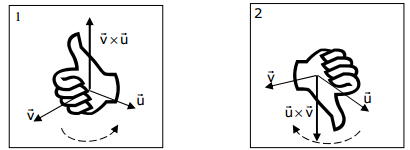
\includegraphics[width=0.4\linewidth]{analitica/imagens/rmd.png}
 \end{figure}
 
 \item $\vec{u} \times \vec{v} = \Vert \vec{u} \Vert \cdot \Vert \vec{v} \Vert \cdot \sin{\theta}$, onde $\theta$ é o ângulo entre os vetores $\vec{u}$ e $\vec{v}$.
\begin{figure}[H]
\centering
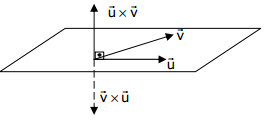
\includegraphics[width=0.4\linewidth]{analitica/imagens/prop.png}
\end{figure}
\end{enumerate}

\textbf{Importante:} Da propriedade (\ref{prop}), $\vec{u} // \vec{v} \quad \Leftrightarrow \quad \vec{u} \times \vec{v}=0$

\section{Interpretação geométrica do módulo do produto vetorial}

O módulo do produto vetorial de dois vetores $\vec u$ e $\vec v$ é igual a área do paralelogramo cujos lados são determinado pelos vetores $\vec u$ e $\vec v$.

\begin{figure}[H]
\centering
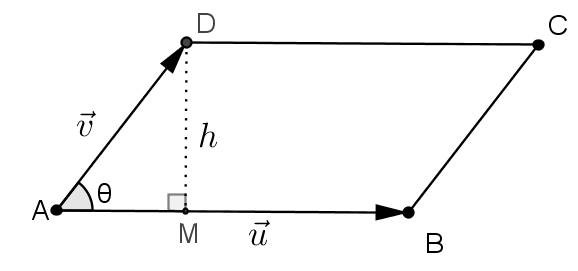
\includegraphics[width=0.4\linewidth]{analitica/imagens/prodvet.png}
\end{figure}

\textbf{Demonstração}: observe inicialmente que o paralelogramo $ABCD$ é determinado pelos vetores $\vec u=\overrightarrow{AB}$ e $\vec v=\overrightarrow{AD}$. Note que a altura do paralelogramo é dada por $h=\Vert v\Vert\cdot \sin{\theta}$

Em todo paralelogramo, a área é dada pela multiplicação da base pela altura, portanto:
\begin{eqnarray*}
A_{ABCD} & = & \Vert\vec u\Vert\cdot h \\
A_{ABCD} & = & \Vert\vec u\Vert\cdot \Vert v\Vert\cdot \sin{\theta} \\
A_{ABCD} & = & \Vert \vec u \times v \Vert
\end{eqnarray*}

Também é possível verificar que a área do triângulo $ABD$ é $$ A_{ABD}= \frac{\Vert\vec u \times v \Vert}{2}$$
\chapter{Produto misto}

\begin{df} Dados os vetores $\vec{u}=(x_1, y_1, z_1)$, $\vec{v}=(x_2, y_2, z_2)$ e $\vec{w}=(x_3, y_3, z_3)$ chama-se produto misto dos vetores $\vec{u}$, $\vec{v}$ e $\vec w$, nesta ordem, ao número real representado por $\vec{u}\cdot (\vec{v}\times \vec w)$ ou $$(\vec{u}, \vec{v}, \vec w)= \left|
\begin{array}{ccc}
x_1 & y_1 & z_1 \\
x_2 & y_2 & z_2 \\
x_3 & y_3 & z_3 \\
\end{array}
\right|$$

O produto misto não está definido no $\mathbb{R}^2$.
\end{df} 

\section{Propriedades do produto misto}

\begin{enumerate}[(1)]
 \item $(u,v,w)=0$ se um dos vetores é nulo, se dois deles são colineares, ou se os três são coplanares.
 \item Na permutação de dois dos três vetores, o produto misto $(u,v,w)$  muda de sinal.
 \item $\alpha(u,v,w)= (\alpha u,v,w)=(u,\alpha v,w)=(u,v,\alpha w)$, com $\alpha \in \mathbb{R}$.
\end{enumerate}

\subsection{Vetores coplanares}

Vetores coplanares são vetores que possuem representantes num mesmo plano.
\begin{enumerate}[a)]
 \item Dois vetores são sempre coplanares.
 \item Três vetores $\vec u$, $\vec v$ e $\vec w$ do $\mathbb{R}^3$ são coplanares se $(u,v,w)=0$.
 \item Três vetores $\vec u$, $\vec v$ e $\vec w$ do $\mathbb{R}^3$ são coplanares se $\vec u=a\vec v + b\vec w$.
 \item Quatro pontos do $\mathbb{R}^3$ são coplanares se três vetores quaisquer escolhidos dentre eles são coplanares.
\end{enumerate}

\section{Interpretação geométrica do módulo do produto misto}

O módulo do produto misto (u,v,w) é igual ao volume do paralelepípedo cujas arestas são determinadas 
pelos vetores  u, v e 

\begin{figure}[H]
\centering
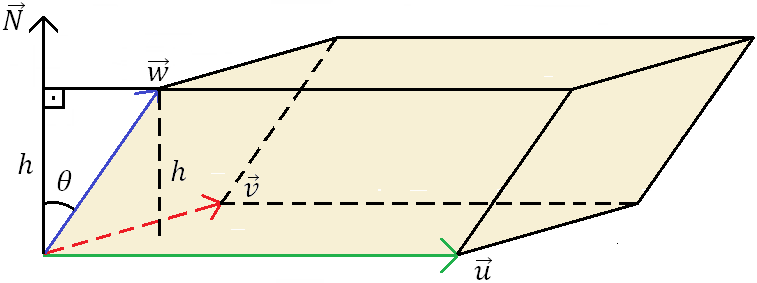
\includegraphics[width=0.4\linewidth]{analitica/imagens/misto.png}
\end{figure}

\textbf{Demonstração}: observe inicialmente que o volume do paralelepípedo é dado pela multiplicação da área da base pela altura $h$. A base é um paralelogramo determinado pelos vetores $\vec u$ e $\vec v$, cuja área é dada por $\vec u \times \vec v$. Note que a altura é dada por $h=\Vert \vec w \Vert \cdot|\cos{\theta}|$.

\begin{eqnarray*}
V & = & (\textrm{área da base})\cdot h \\
V & = & \Vert \vec u \times \vec v\Vert \cdot \Vert w\Vert\cdot |\cos{\theta}|\\
V & = & |\vec w  \cdot ( \vec u \times \vec v)|\\
V & = & |(\vec w, \vec u, \vec v )|
\end{eqnarray*}
\chapter{Retas}

\section{Equações da reta}

Uma reta $r$ pode ser representada por diferentes equações.

\subsection{Equação vetorial da reta}

Seja $A$ um ponto de uma reta $r$ que tem a direção de um vetor $v\neq 0$. Se um ponto $P$ pertence a $r$ então os vetores $\overrightarrow{AP}$ e $\vec v$ são colineares, isto é, existe um real $t$, tal que $\overrightarrow{AP}=t\vec v$ ou $P=A+t\vec v$.
\begin{multicols}{2}
\begin{figure}[H]
\centering
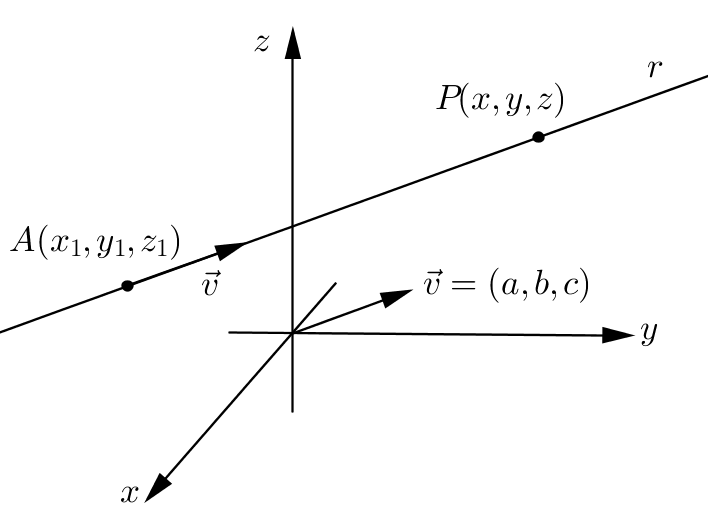
\includegraphics[scale=1]{analitica/imagens/reta-vetorial.png}
\end{figure}

$(x, y, z)=(x_1, y_1, z_1)+t(a,b,c)$

$\vec v$: vetor diretor da reta

$t$: parâmetro
\end{multicols}

\subsection{Equações paramétricas da reta}

Da equação vetorial da reta $r$, vem:

$$r:\left\{ \begin{array}{l}
x=x_1+at\\
y=y_1+bt\\
z=z_1+ct \end{array} \right. $$

\subsection{Equações simétricas da reta}

Admitindo-se $a$, $b$ e $c$ não nulos nas equações paramétricas e isolando o parâmetro $t$, vem:

$$\frac{x-x_1}{a}=\frac{y-y_1}{b}=\frac{z-z_1}{c}$$

\subsection{Equações reduzidas da reta}

Nas equações simétricas, escrevendo-se $y$ como função de $x$ e $z$ como função de $x$, vem:

$$r:\left\{ \begin{array}{l}
y=mx+n\\
z=px+q \end{array} \right. $$

\section{Retas paralelas aos eixos coordenados}

$r\parallel Ox \quad\Longleftrightarrow \quad \vec v \parallel \vec i \quad\Longleftrightarrow \quad r:\left\{ \begin{array}{l}
y=y_1\\
z=z_1 \end{array} \right.$

$r\parallel Oy \quad\Longleftrightarrow \quad \vec v \parallel \vec j \quad\Longleftrightarrow \quad r:\left\{ \begin{array}{l}
x=x_1\\
z=z_1 \end{array} \right.$

$r\parallel Oz \quad\Longleftrightarrow \quad \vec v \parallel \vec k \quad\Longleftrightarrow \quad r:\left\{ \begin{array}{l}
x=x_1\\
y=y_1 \end{array} \right.$


\textbf{Importante:}  Se duas componentes do vetor diretor forem nulas, a reta  é  paralela  ao  eixo  correspondente a componente não nula.

\section{Retas paralelas aos planos coordenados}

$r\parallel xOy \quad\Longleftrightarrow \quad \vec v \perp \vec k \quad\Longleftrightarrow \quad \vec v=(a,b,0) \quad\Longleftrightarrow \quad r:\left\{ \begin{array}{l}
x=x_1+at\\
y=y_1+bt\\
z=z_1 \end{array} \right.$

$r\parallel xOz \quad\Longleftrightarrow \quad \vec v \perp \vec j \quad\Longleftrightarrow \quad \vec v=(a,0,c) \quad\Longleftrightarrow \quad r:\left\{ \begin{array}{l}
x=x_1+at\\
y=y_1\\
z=z_1+ct \end{array} \right.$

$r\parallel yOz \quad\Longleftrightarrow \quad \vec v \perp \vec i \quad\Longleftrightarrow \quad \vec v=(0,b,c) \quad\Longleftrightarrow \quad r:\left\{ \begin{array}{l}
x=x_1\\
y=y_1+bt\\
z=z_1+ct \end{array} \right.$

\textbf{Importante:} Se uma das componentes do vetor diretor é nula, a reta é  paralela  ao  plano correspondente as componentes não nulas.

\section{Ângulo de duas retas}

O ângulo entre duas retas é o menor ângulo formado por dois vetores diretores das retas.

Se $\vec u$ e $\vec v$ são os vetores diretores das retas $r$ e $s$, então o ângulo entre as retas será dado por $\theta$, onde: $$\cos{\theta}=\frac{|\vec u \cdot \vec v|}{\Vert \vec u \Vert \Vert \vec v \Vert} \qquad 0\leq \theta \leq \frac{\pi}{2}$$

\subsection{Retas paralelas}

$r_1\parallel r_2 \quad\Longleftrightarrow \quad \vec v_1 \parallel \vec v_2$

\subsection{Retas ortogonais}

$r_1\perp r_2 \quad\Longleftrightarrow \quad \vec v_1 \perp \vec v_2$

\subsection{Reta ortogonal a duas retas}

Seja $r$ é uma reta ortogonal à duas retas não paralelas $r_1$ e $r_2$ com vetores diretores $\vec v_1$ e $\vec v_2$.

O vetor diretor de $r$ é qualquer vetor com a direção de $\vec v=\vec v_1 \times \vec v_2$.


\section{Intersecção de duas retas}

Sejam $r$ e $s$ duas retas concorrentes, então o ponto de intersecção $I$, é a solução do sistema formado pelas equações das retas $r$ e $s$.

\section{Retas coplanares}

Duas retas são coplanares se são paralelas ou concorrentes.

\textbf{Observação:} Duas retas não-coplanares são chamadas reversas

\textbf{Importante:} Retas perpendiculares são retas ortogonais e coplanares.
\chapter{Planos}

\section{Equação geral do plano}

Seja $A$ um ponto de um plano $\pi$ e $\vec n$ um vetor não nulo ortogonal a $\pi$. Um ponto $P$ pertence a $\pi$ se os vetores $\vec n$ e $\overrightarrow{AP}$ são ortogonais, isto é, $\vec n \cdot \overrightarrow{AP}=0$.

\begin{multicols}{2}
\begin{figure}[H]
\centering
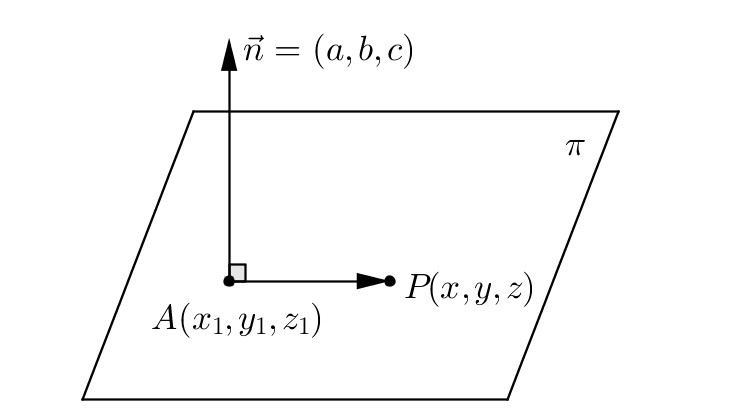
\includegraphics[scale=1]{analitica/imagens/plano.png}
\end{figure}

$$\pi: ax + by + cz + d = 0$$

\end{multicols}


\section{Equação vetorial do plano}

Sejam $A$ um ponto de um plano $\pi$ e, $\vec u$ e $\vec v$ são dois vetores não colineares paralelos a $\pi$. Se o ponto $P$ pertence ao plano $\pi$ então existem dois números reais $h$ e $t$, tais que $\overrightarrow{AP}=h\vec u+t\vec v$ ou $P=A+h\vec u+t\vec v$.

\begin{multicols}{2}
\begin{figure}[H]
\centering
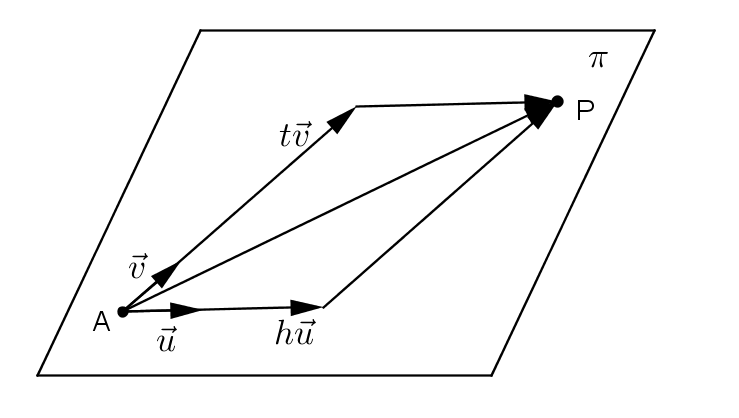
\includegraphics[scale=1]{analitica/imagens/plano-vet.png}
\end{figure}

$(x,y,z)=(x_1,y_1,z_1)+h(a_1,b_1,c_1)+t(a_2,b_2,c_2)$
\end{multicols}

\section{Equações paramétricas do plano}

Da equação vetorial do plano, vem:

$$\left\{ \begin{array}{l}
x=x_1+a_1h+a_2t\\
y=y_1+b_1h+b_2t\\
z=z_1+c_1h+c_2t \end{array} \right. $$

\section{Planos paralelos aos eixos coordenados}

\begin{enumerate}[(a)]
 \item Se um plano $\pi$ é paralelo ao eixo $Ox$, o seu vetor normal $\vec n$ é ortogonal ao vetor $\vec i$, e  portanto $\vec n=(0,b,c)$. Neste caso, a equação de $\pi$  tem a forma $by + cz + d = 0$.
 \item Se um plano $\pi$ é paralelo ao eixo $Oy$, o seu vetor normal $\vec n$ é ortogonal ao vetor $\vec j$, e  portanto, $\vec n=(a,0,c)$. Neste caso, a equação de $\pi$ tem a forma $ax+cz+d=0$.
 \item Se um plano $\pi$ é paralelo ao eixo $Oz$, o seu vetor normal $\vec n$ é ortogonal ao vetor $\vec k$, e portanto, $\vec n=(a,b,0)$. Neste caso, a equação de $\pi$ tem a forma $ax+by+d=0$.
\end{enumerate}

\textbf{Importante:} Se uma das componentes do vetor normal é nula, o plano é paralelo ao eixo correspondente a componente nula (a variável ausente na equação, indica o eixo ao qual o plano é paralelo).

\section{Planos paralelos aos planos coordenados}

\begin{enumerate}[(a)]
 \item Se um plano $\pi$ é paralelo ao plano $xOy$, qualquer vetor normal $\vec n$ tem a direção do vetor $\vec k$, e portanto, $\vec n=(0,0,c)$. Neste caso, a equação de $\pi$ tem a forma $cz+d=0$.
 \item Se um plano $\pi$ é paralelo ao plano $xOz$, qualquer vetor normal $\vec n$ tem a  direção do vetor $\vec j$,e portanto, $\vec n=(0,b,0)$. Neste caso, a equação de $\pi$ tem a forma $by+d=0$.
 \item Se um plano $\pi$ é paralelo ao plano $yOz$, qualquer vetor normal $\vec n$ tem a direção do vetor $\vec i$, e portanto, $\vec n=(a,0,0)$. Neste caso, a equação de $\pi$ tem a forma $ax+d=0$.
\end{enumerate}

\textbf{Importante:} Se duas componentes do vetor normal forem nulas, o plano é  paralelo ao plano correspondente as componentes nulas (as variáveis ausentes na equação, indicam o plano coordenado ao qual o plano é paralelo).

\section{Ângulo de dois planos}

O ângulo entre dois planos $\pi_1$ e $\pi_2$ é a medida do ângulo entre duas retas $r_1$ e $r_2$, respectivamente, perpendiculares a $\pi_1$ e $\pi_2$.

\begin{multicols}{2}
\begin{figure}[H]
\centering
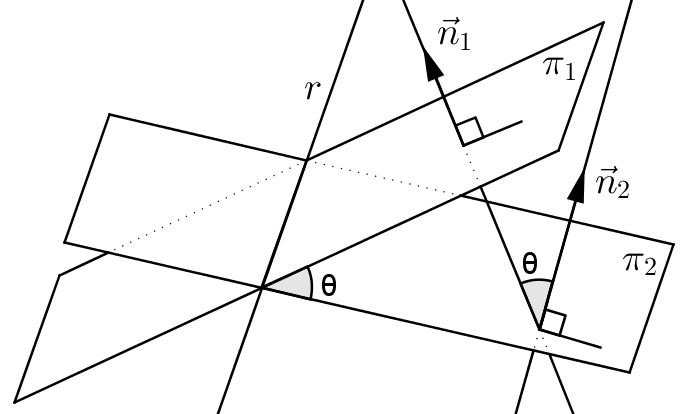
\includegraphics[scale=1]{analitica/imagens/planos-ang.png}
\end{figure}

$$\cos{\theta}=\frac{|\vec n_1 \cdot \vec n_2|}{\Vert \vec n_1 \Vert \Vert \vec n_2 \Vert} \qquad 0\leq \theta \leq \frac{\pi}{2}$$

\end{multicols}

$\pi_1\parallel \pi_2 \quad\Longleftrightarrow \quad \vec n_1 \parallel \vec n_2$

$\pi_1\perp \pi_2 \quad\Longleftrightarrow \quad \vec n_1 \perp \vec n_2$

\section{Intersecção de dois planos}

\begin{multicols}{2}
\begin{figure}[H]
\centering
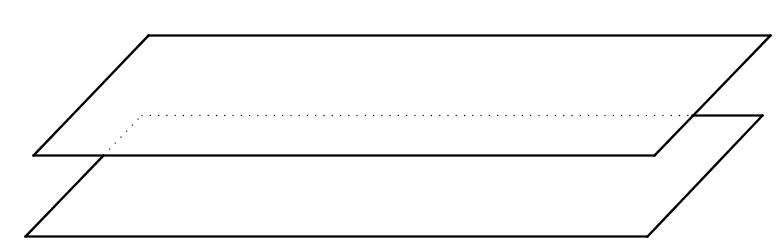
\includegraphics[scale=1]{analitica/imagens/planos-par.png}
\end{figure}

\noindent Planos paralelos não possuem intersecção.

\end{multicols}

\begin{multicols}{2}
\begin{figure}[H]
\centering
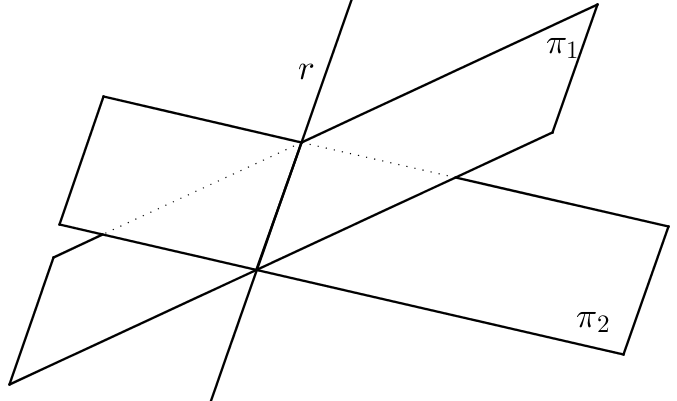
\includegraphics[scale=1]{analitica/imagens/planos-inter.png}
\end{figure}

\noindent A intersecção dos planos $\pi_1$ e $\pi_2$ é a reta $r$ cujas equações são obtidas resolvendo-se o sistema formado pelas equações de $\pi_1$ e $\pi_2$.

$$\left\{ \begin{array}{l} \pi_1: a_1x+b_1y+c_1z+d_1=0\\   \pi_2: a_2x+b_2y+c_2z+d_2=0 \end{array} \right.$$


\end{multicols}




\textbf{Observação:} Sejam $\left\{ \begin{array}{l} y=mx+n\\   z=px+q \end{array} \right.$ as equações reduzidas da reta $r$, intersecção dos planos $\pi_1$ e $\pi_2$. Cada equação de $r$ pode ser obtida através da  eliminação no sistema acima da variável ausente na equação.

\section{Ângulo de uma reta com um plano}

O ângulo $\phi$, da reta $r$ com o plano é o complementar do ângulo entre a reta $r$ e uma reta $s$ perpendicular a $\pi$, com $0\leq \phi \leq \frac{\pi}{2}$.


\begin{multicols}{2}
\begin{figure}[H]
\centering
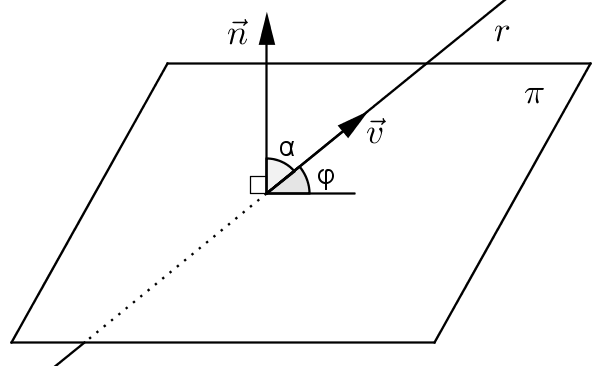
\includegraphics[scale=1]{analitica/imagens/plano-reta-a.png}
\end{figure}

$$\cos{\alpha}=\frac{|\vec v \cdot \vec n|}{\Vert \vec v \Vert \Vert \vec n \Vert}$$

$$\phi=\frac{\pi}{2}-\alpha$$

\end{multicols}




\section{Intersecção de reta com plano}

\begin{multicols}{2}
\begin{figure}[H]
\centering
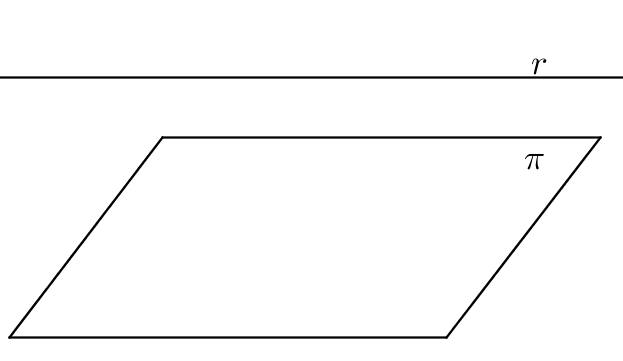
\includegraphics[scale=1]{analitica/imagens/plano-reta2.png}
\end{figure}

\noindent Quando a reta $r$ for paralela ao plano $\pi$, então não haverá interseção entre reta e plano. Neste caso, o sistema formado pelas equações da reta $r$ e do plano $\pi$ não possuirá solução.
\end{multicols}

\begin{multicols}{2}
\begin{figure}[H]
\centering
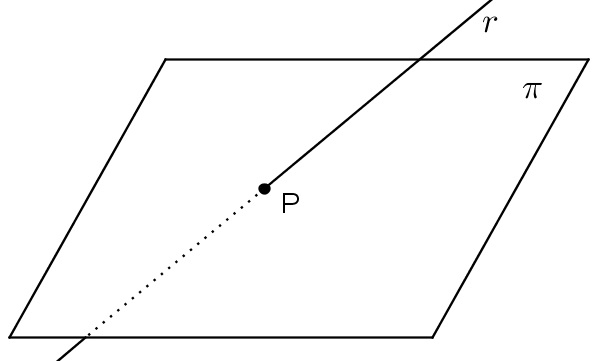
\includegraphics[scale=1]{analitica/imagens/plano-reta.png}
\end{figure}

\noindent Quando a reta $r$ for concorrente ao plano $\pi$, então a intersecção entre plano e reta será um ponto $P$. As coordenadas deste ponto são obtidas com a solução do sistema formado pelas equações da reta $r$ e do plano $\pi$.
\end{multicols}

Há ainda a situação em que a reta $r$ está contida no plano, e neste caso, todos os pontos da reta estarão no plano. Neste caso, o sistema formado pelas equações da reta $r$ e do plano $\pi$ será considerado indeterminado, pois possuirá infinitas soluções.
\chapter{Distâncias}

Neste tópico, abordaremos algumas relações importantes para obtenção das distâncias enter elementos do $\mathbb{R}^3$.

\section{Distância entre dois pontos}

Se considerarmos dois pontos $A(x_1, y_1, z_1)$ e $B(x_2, y_2, z_2)$ do $\mathbb{R}^3$, então a distância entre estes pontos é definida por
\begin{equation}
d(A, B)=\sqrt{(x_2-x_1)^2+(y_2-y_1)^2+(z_2-z_1)^2}
\end{equation}

\begin{exemplo} Qual a distância entre os pontos $P(-1, 2, 0)$ e $Q(3, 2, -1)$?

Basta utilizar a relação acima
\begin{eqnarray*}
d(P, Q)   & = & \sqrt{(x_2-x_1)^2+(y_2-y_1)^2+(z_2-z_1)^2} \\
          & = &  \sqrt{(3+1)^2+(2-2)^2+(-1-0)^2} \\
          & = &  \sqrt{4^2+0^2+(-1)^2} \\
          & = &  \sqrt{16+0+1} \\
          & = & \sqrt{17}
\end{eqnarray*}

\end{exemplo}

\section{Distância de um ponto a uma reta}

Para obter a distância entre um ponto $P$ a uma reta $r$, precisamos considerar o vetor diretor $\vec{v}$ da reta e um ponto $A$ qualquer sobre a reta $r$. A distância entre a reta $r$ e o ponto $P$ será obtida através da da seguinte relação
\begin{equation} 
d(P, r)=\frac{\|\vec{v}\times \overrightarrow{AP}\|}{\|\vec{v}\|}
\label{distpr}
\end{equation}

\begin{exemplo} 
Determine a distância do ponto $P(1, 0, -2)$ a reta $r: \left\{
\begin{array}{l}
x=3+4t \\
y=-2-t \\
z=4+t \\
\end{array} \right.$

Observe que o vetor diretor da reta $r$ é $\vec{v}=(4,-1,1)$, e $\|v\|=\sqrt{4^2+(-1)^2+1^2}=\sqrt{16+1+1}=\sqrt{18}=3\sqrt{2}$.

Obtenha um ponto qualquer da reta $r$, por exemplo para $t=0$ temos o ponto $A(3,-2,4)$. E então o vetor $\overrightarrow{AP}$ será $\overrightarrow{AP}=P-A=(-2,2,-6)$.

$\vec{v} \times \overrightarrow{AP}= \left|
\begin{array}{ccc|cc}
\vec i & \vec j & \vec k & \vec i & \vec j \\
4 & -1 & 1 &4 & -1 \\
-2 & 2 & -6 &-2 & 2 \\
\end{array}
\right|= 4\vec{i} +22\vec{j} +6\vec{k}
$

E portanto temos $\|v \times \overrightarrow{AP}\|=\sqrt{4^2+22^2+6^2}=\sqrt{16+484+36}=\sqrt{536}=2\sqrt{134}$

E agora, utilizando a expressão \ref{distpr}, temos $d(P, r)=\frac{\|\vec{v}\times \overrightarrow{AP}\|}{\|\vec{v}\|}=\frac{2\sqrt{134}}{3\sqrt{2}}=\frac{4\sqrt{67}}{3}$.
\end{exemplo}

\section{Distância de um ponto a um plano}

A distância entre o ponto $P_0(x_0, y_0, z_0)$ e o plano $\pi: ax+by+cz+d=0$ é dada por: 
\begin{equation}
d(P_0, \pi)=\frac{|ax_0+by_0+cz_0+d|}{\sqrt{a^2+b^2+c^2}}
\end{equation}

\begin{exemplo} Obtenha a distância do ponto $A(1, 2, -5)$ ao plano $\pi: 12x+3y-4z+7=0$. 

Aplicando a relação acima, temos:
\begin{eqnarray*}
d(P_0, \pi) & = &\frac{|ax_0+by_0+cz_0+d|}{\sqrt{a^2+b^2+c^2}} \\
d(A, \pi) & = & \frac{|12x_0+3y_0-4z_0+7|}{\sqrt{12^2+3^2+(-4)^2}} \\
          & = &  \frac{|12\cdot 1+3\cdot 2-4\cdot (-5)+7|}{\sqrt{169}} \\
          & = & \frac{|12+6+20+7|}{13}= \frac{45}{13}
\end{eqnarray*}

\end{exemplo}

\section{Distância entre duas retas}

Consideremos o caso em que as duas retas $r$ e $s$ são reversas. Vamos considerar $P$ um ponto da reta $r$, e $\vec{v}_r$ o seu vetor diretor. Da mesma forma, $Q$ é um ponto da reta $s$ e $\vec{v}_s$ seu vetor diretor.

Desta forma, através das propriedades do produto misto, temos:
\begin{equation}
d(r, s)=\frac{|(\vec{v}_r, \vec{v}_s, \overrightarrow{PQ})|}{\| \vec{v}_r \times \vec{v}_s \|} \label{distrs}
\end{equation}

Se duas retas são paralelas, a distância entre elas é definida pela distância de um ponto de uma delas até a outra reta. Ou seja, se resume a um problema de distância entre ponto e reta.

\begin{exemplo} Obtenha a distância entre as retas $\displaystyle r: \frac{x-2}{3}=1-z \; ; \; y=2$ e $s:\left\{ \begin{array}{l}
y=4-2x\\
z=3x+1 \end{array} \right. $.

Na reta $r$ temos o vetor diretor $\vec{v}_r=(3,0,-1)$ e escolhemos um ponto qualquer, por exemplo, $P(2,2,1)$. Na reta $s$ temos o vetor diretor $\vec{v}_s=(1,-2,3)$ e escolhemos um ponto qualquer, por exemplo, $Q(2,0,7)$.

Assim, temos o vetor $\overrightarrow{PQ}=Q-P=(0,-2,6)$

$(\vec{v}_r, \vec{v}_s, \overrightarrow{PQ})= \left|
\begin{array}{ccc|cc}
3 & 0 & -1 & 3 & 0 \\
1 & -2 & 3 &1 & -2 \\
0 & -2 & 6 &0 & -2 \\
\end{array}
\right|= -16
$

$\vec{v}_r \times \vec{v}_s= \left|
\begin{array}{ccc|cc}
\vec i & \vec j & \vec k & \vec i & \vec j \\
3 & 0 & -1 & 3 & 0 \\
1 & -2 & 3 &1 & -2 \\
\end{array}
\right|= -2\vec{i} -10\vec{j} -6\vec{k}
$

Calculamos $\|\vec{v}_r \times \vec{v}_s\|=\sqrt{(-2)^2+(-10)^2+(-6)^2}=\sqrt{4+100+36}=\sqrt{140}=2\sqrt{35}$

E agora basta utilizar a relação \ref{distrs}, e obter a distância entre as retas $r$ e $s$:

$ d(r, s)=\frac{|(\vec{v}_r, \vec{v}_s, \overrightarrow{PQ})|}{\| \vec{v}_r \times \vec{v}_s \|}=\frac{|-16|}{2\sqrt{35}}=\frac{8}{\sqrt{35}}=\frac{8\sqrt{35}}{35}$

\end{exemplo}

\section{Distância entre uma reta e um plano}

Se uma reta e um plano não forem paralelos, então a distância ente eles será $0$ (zero), pois sempre terão um ponto de interseção.

No caso de uma reta paralela a um plano, basta considerar um único ponto da reta em questão, e calcular a distância deste ponto ao plano dado.

\section{Distância entre dois planos}

Se dois planos são paralelos, basta considerar o ponto de um dos planos, e calcular a distância deste ponto ao outro plano.

Se os planos não são paralelos, então a distância será $0$ (zero) pois os mesmos terão interseção.
\chapter{Cônicas}

A fórmula da distância entre dois pontos é muitas vezes usada para achar a equação de uma curva cuja definição geométrica depende de uma ou mais distâncias. Um das curvas mais simples desta espécie é a circunferência, mas outras curvas como parábolas, elipses e hipérboles também estão relacionadas a distâncias entre elementos geométricos (pontos, retas).

\section{Parábola}
Curva do plano formada pelos pontos equidistantes de um ponto fixo $F$ (foco) e de uma reta $d$ (diretriz). Ou seja, um ponto $P(x, y)$ pertence à parábola, se e somente se, $$d(P, F)=d(P, d)$$

Uma parábola possui os seguintes elementos:
\begin{itemize}
  \item \textbf{foco:} é o ponto $F$.
  \item \textbf{diretriz:} é a reta $d$.
  \item \textbf{eixo:} é a reta que passa por $F$ e é perpendicular a $d$. Observe que toda parábola é simétrica em relação ao seu eixo.
  \item \textbf{vértice:} é o ponto V de interseção da parábola com o seu eixo.
\end{itemize}

Para este texto, chamaremos a distância entre o foco $F$ e a reta diretriz $d$ por parâmetro da parábola e será dado por: $p=d(F, d)$. Observe que a distância entre o vértice e a reta diretriz, e o vértice e o foco são metade deste valor, ou seja $\displaystyle d(V, d)=d(V, F)= \frac{p}{2}$.

\subsection{Parábola com eixo vertical}

Inicialmente vamos considerar a parábola com eixo vertical, ou seja, o eixo é paralelo ao eixo $Oy$. Mais particularmente, consideremos o próprio eixo $Oy$ como eixo da parábola, e o vértice sendo $V(0, 0)$.

Neste caso, o foco F será um ponto sobre o eixo $Oy$, e possuirá coordenadas $\displaystyle F(0, \frac{p}{2})$. A reta diretriz será dada pela equação $y=-\frac{p}{2}$.

A parábola será dada pelos pontos $P(x, y)$, de modo que\footnote{Observe que ponto da projeção de $P$ sobre $d$ será dado por $P'(x,-\frac{p}{2})$.}:
\begin{eqnarray*}
d(P, F) & = & d(P, d)   \\
d(P, F) & = & d(P, P')   \\
\sqrt{(x-0)^2+\left(y-\frac{p}{2}\right) ^2} & = & \sqrt{(x-x)^2+\left(y+\frac{p}{2}\right)^2}  \\
x^2+\left(y-\frac{p}{2}\right)^2 & = & 0^2+\left(y+\frac{p}{2}\right)^2  \\
x^2+y^2-py+\frac{p^2}{4} & = & y^2+py+\frac{p^2}{4} \\
x^2 & = & 2py 
\end{eqnarray*}

Ou seja, a equação reduzida da parábola com vértice $V(0, 0)$, foco $\displaystyle F(0,\frac{p}{2})$ e diretriz $\displaystyle y=-\frac{p}{2}$ será dada por: $$x^2=2py$$

\begin{figure}[H]
\centering
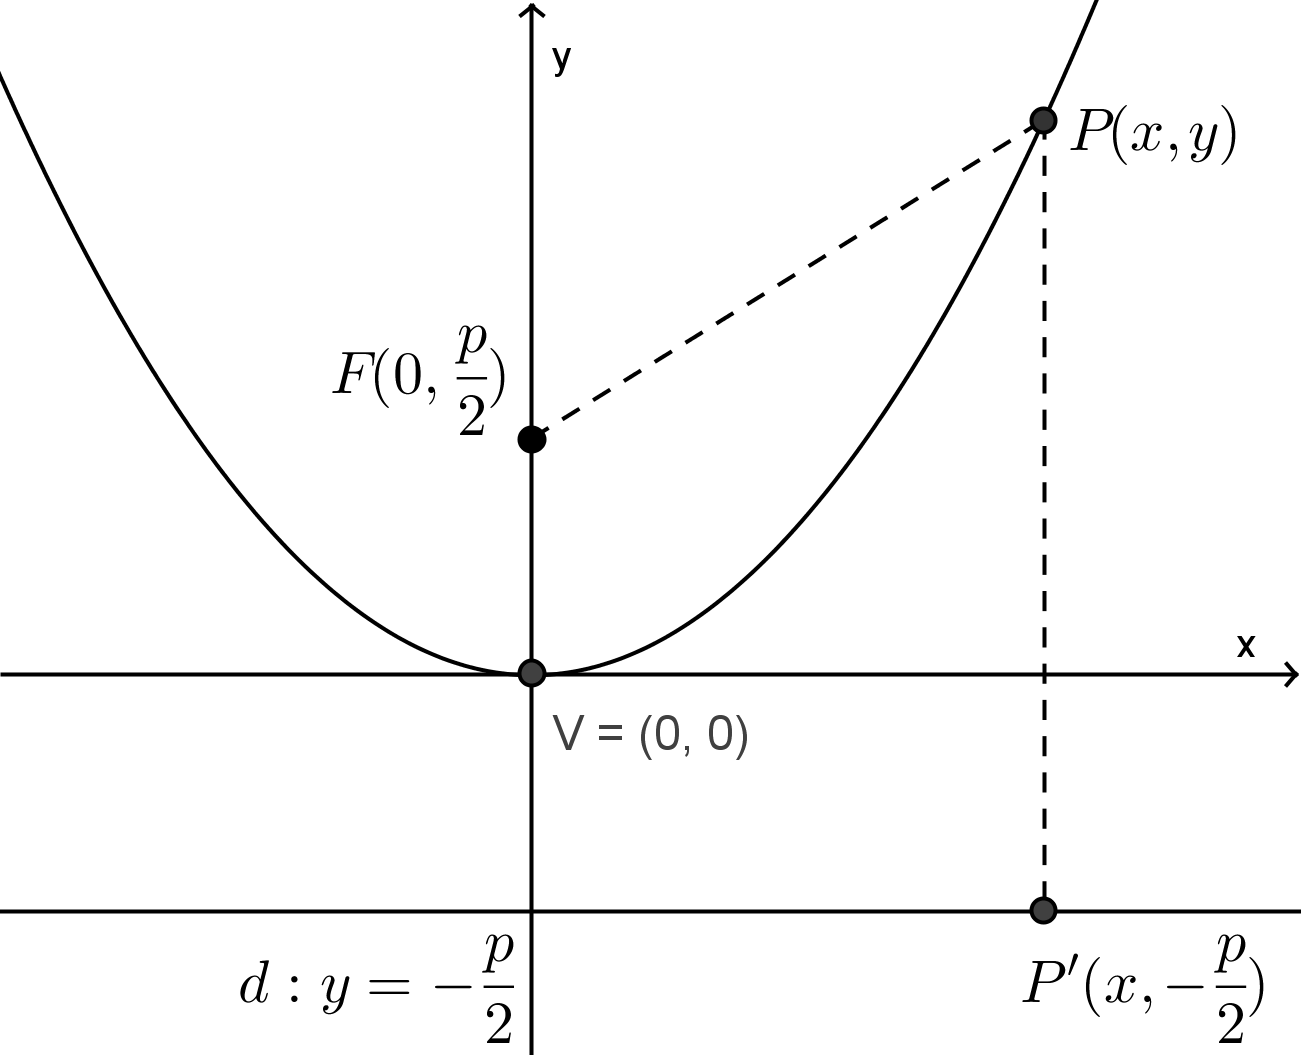
\includegraphics[width=0.4\linewidth]{analitica/imagens/parabolav1.png}
\caption{Parábola com eixo $Oy$}
\label{fig:para1}
\end{figure}

Observe que:
\begin{itemize}
  \item $p>0$: concavidade (abertura) da parábola para cima.
  \item $p<0$: concavidade (abertura) da parábola para baixo.
\end{itemize}

Mais genericamente, se considerarmos como eixo da parábola, qualquer reta vertical paralela a $Oy$, considerando o vértice $V(h, k)$, teremos a equação: $$(x-h)^2=2p(y-k)$$

%\begin{multicols}{2}

\begin{exemplo} Obtenha a equação da parábola com vértice $V(-1, 2)$, eixo paralelo ao eixo $Oy$, e que $d(F, V)=1$.

Primeiramente devemos observar que $d(F, V)=\frac{p}{2}$, e portanto:
\begin{eqnarray*}
\frac{p}{2} & = & d(F, V)   \\
\frac{p}{2} & = & 1   \\
p & = & 2
\end{eqnarray*}

Como a equação é paralela ao eixo $Oy$, então sua equação é da forma:
\begin{eqnarray*}
(x-h)^2&=&2p(y-k)  \\
(x+1)^2&=&4(y-2)
\end{eqnarray*}


\begin{figure}[H]
\centering
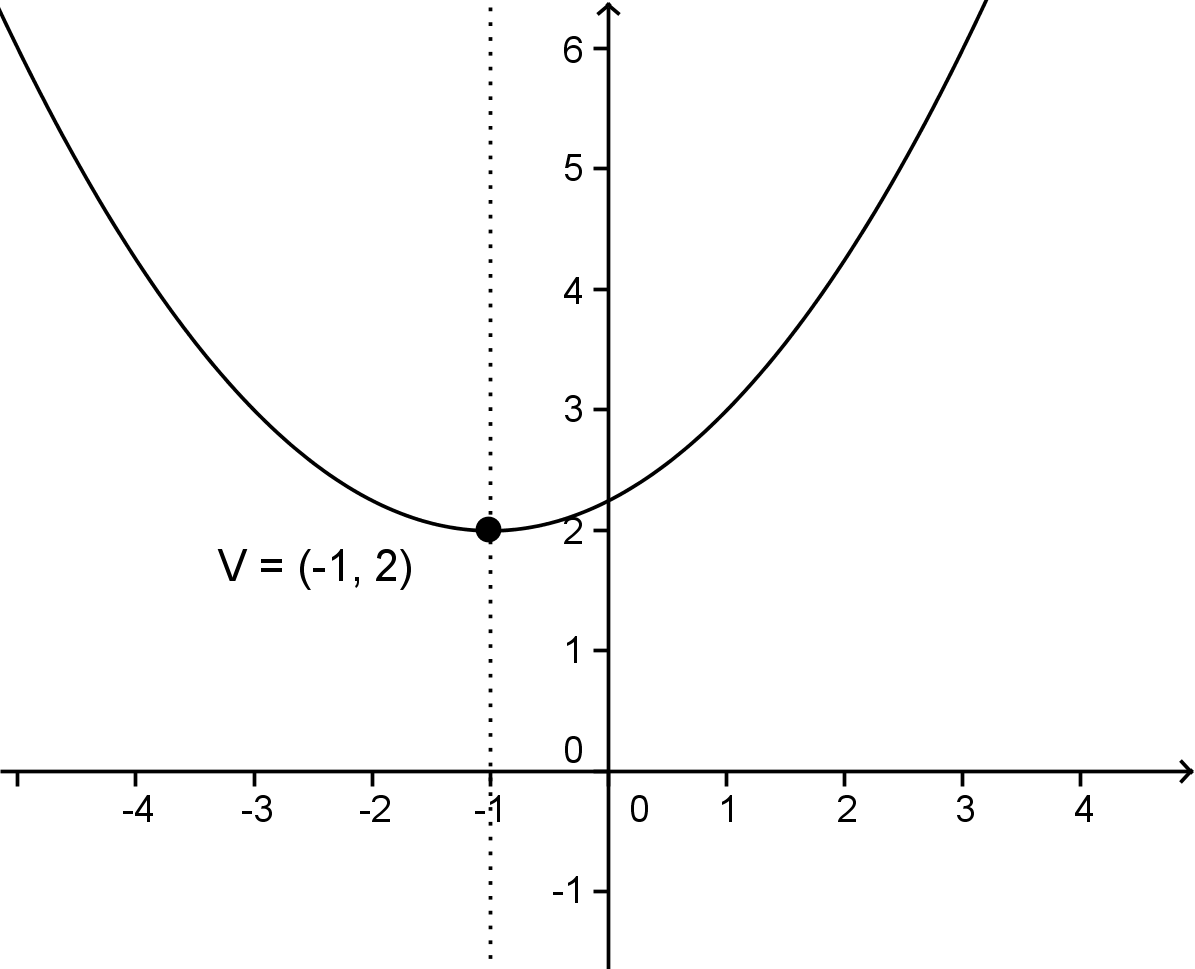
\includegraphics[width=0.4\linewidth]{analitica/imagens/exemplo1.png}
%\caption{Circunferência}
\label{fig:exe1}
\end{figure}

A equação acima ainda pode receber a forma chamada de \textit{equação geral}
\begin{eqnarray*}
(x+1)^2&=&4(y-2) \\
x^2+2x+1&=&4y-8 \\
x^2+2x-4y+9&=&0
\end{eqnarray*}


Se isolarmos o $y$, temos a forma chamada de \textit{equação explícita}
\begin{eqnarray*}
0&=&x^2+2x-4y+9 \\
4y&=&x^2+2x+9 \\
y&=&\frac{x^2}{4}+\frac{x}{2}+\frac{9}{4}
\end{eqnarray*}


\end{exemplo}
%\end{multicols}


\subsection{Parábola com eixo horizontal}

Agora, vamos considerar a parábola com eixo horizontal, ou seja, o eixo é paralelo ao eixo $Ox$. Mais particularmente, consideremos o próprio eixo $Ox$ como eixo da parábola, e o vértice sendo $V(0, 0)$. Neste caso, o foco F será um ponto sobre o eixo $Ox$, e possuirá coordenadas $\displaystyle F\left(\frac{p}{2}, 0\right)$. A reta diretriz será dada pela equação $\displaystyle x=-\frac{p}{2}$.

A parábola será dada pelos pontos $P(x, y)$, de modo que\footnote{Observe que ponto da projeção de $P$ sobre $d$ será dado por $P'(-\frac{p}{2},y)$.}:

\begin{eqnarray*}
d(P, F) & = & d(P, d)   \\
d(P, F) & = & d(P, P')   \\
\sqrt{\left(x-\frac{p}{2}\right)^2+(y-0)^2} & = & \sqrt{\left(x+\frac{p}{2}\right)^2+(y-y)^2}  \\
\left(x-\frac{p}{2}\right)^2+y^2 & = & \left(x+\frac{p}{2}\right)^2+0^2  \\
x^2-px+\frac{p^2}{4}+y^2 & = & x^2+px+\frac{p^2}{4}   \\
y^2 & = & 2px 
\end{eqnarray*}

Ou seja, a equação reduzida da parábola com vértice $V(0, 0)$, foco $F(\frac{p}{2},0)$ e diretriz $\displaystyle x=-\frac{p}{2}$ será dada por: $$y^2=2px$$

\begin{figure}[H]
\centering
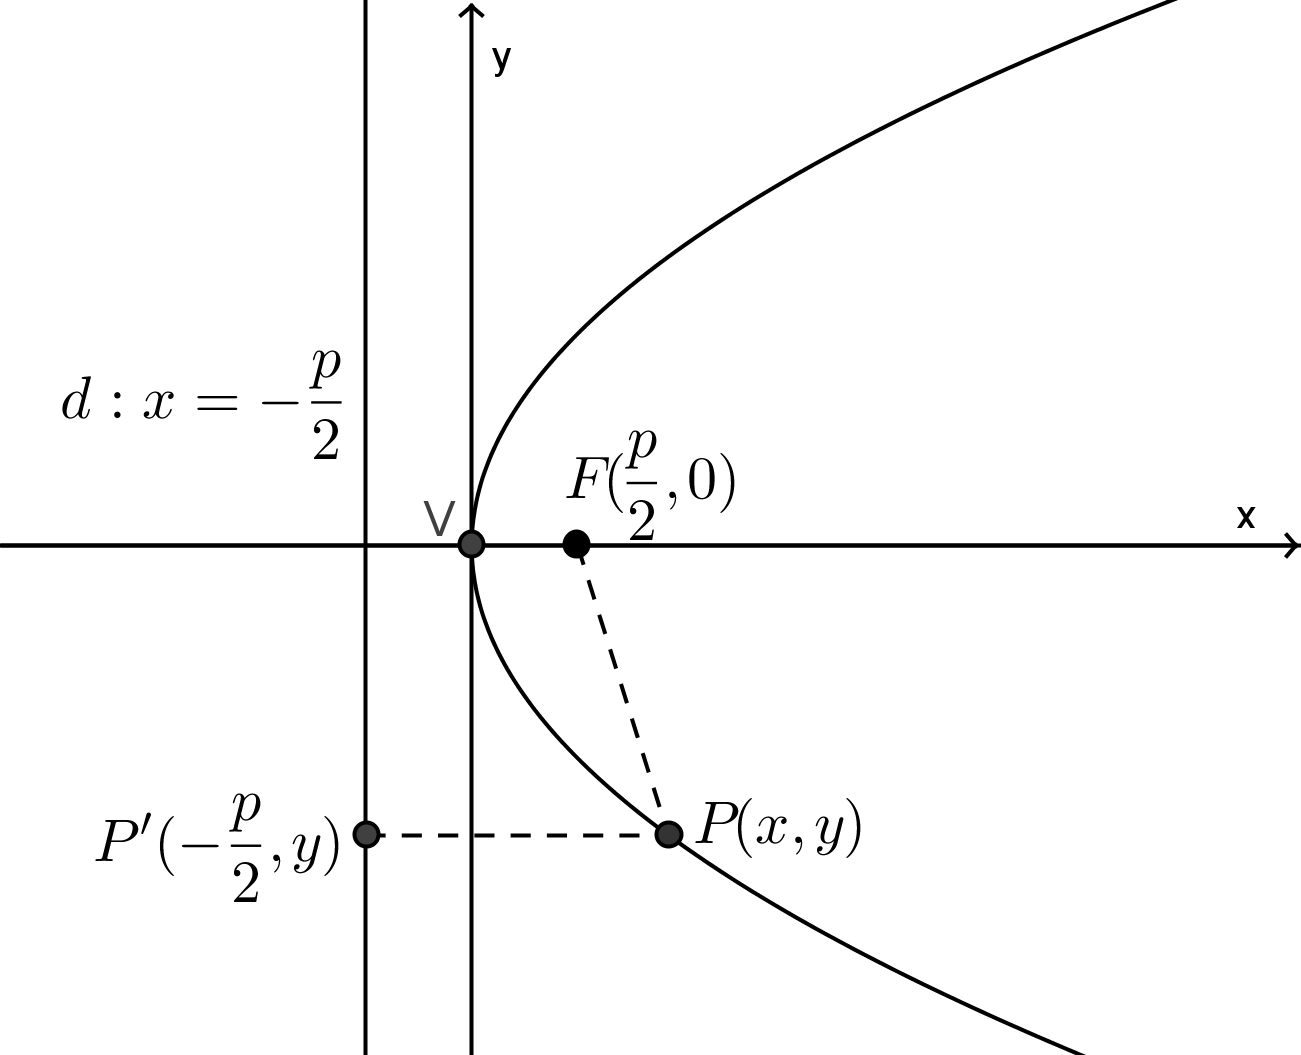
\includegraphics[width=0.5\linewidth]{analitica/imagens/parabolah1.png}
\caption{Parábola com eixo $Ox$}
\label{fig:parah1}
\end{figure}

Observe que:
\begin{itemize}
  \item $p>0$: concavidade (abertura) da parábola para direita.
  \item $p<0$: concavidade (abertura) da parábola para esquerda.
\end{itemize}

Mais genericamente, se considerarmos como eixo da parábola, qualquer reta horizontal paralela a $Ox$, considerando o vértice $V(h, k)$, teremos a equação: $$(y-k)^2=2p(x-h)$$

\section{Circunferência}

A circunferência pode ser definida como o conjunto de todos os pontos que equidistam de um ponto fixo $C$. O ponto fixo é chamado centro da circunferência e a distância de qualquer de seus pontos ao centro é o raio dessa circunferência. Se o centro é o ponto $C(a, b)$ e o raio é o número positivo $r$, e se $P(x, y)$ é um ponto qualquer da circunferência, então a definição acima se traduz

\begin{multicols}{2}
\begin{figure}[H]
\centering
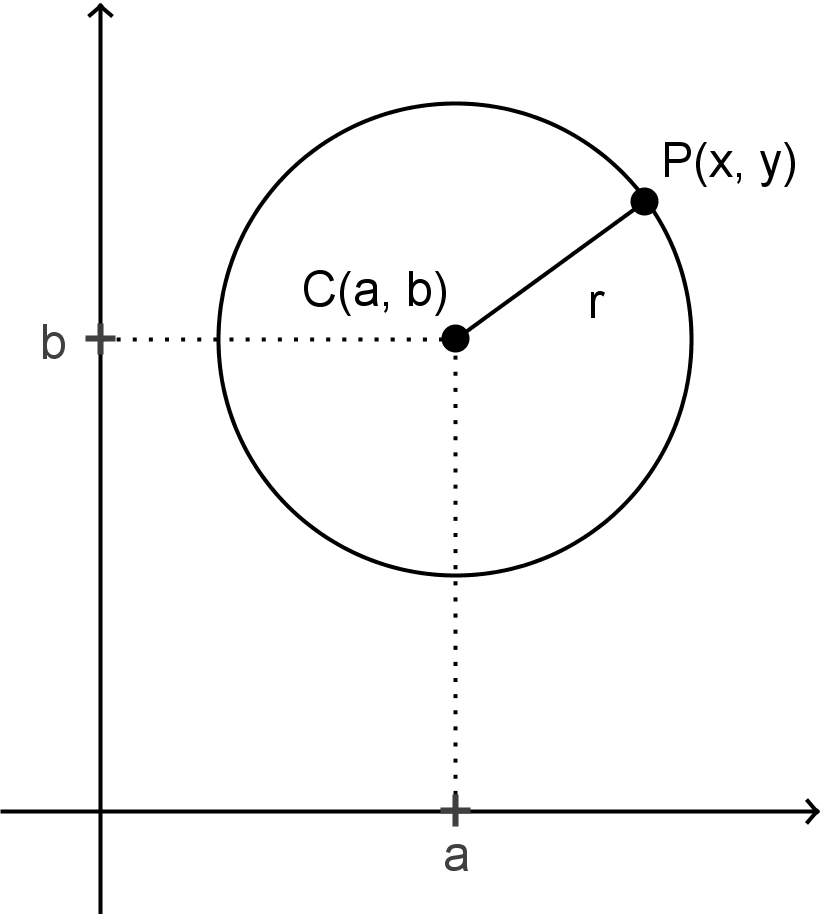
\includegraphics[width=0.45\linewidth]{analitica/imagens/circ1.png}
\caption{Circunferência}
\label{fig:circ1}
\end{figure}

\begin{eqnarray*}
d(P, C) & = & r   \\
\sqrt{(x-a)^2+(y-b)^2} & = & r  \\
(x-a)^2+(y-b)^2 & = & r^2
\end{eqnarray*}
\end{multicols}


Ou seja, a circunferência de centro $C(a, b)$ e raio $r$ é dada por $$(x-a)^2+(y-b)^2= r^2$$

\section{Elipse}

Elipse é o conjunto de todos os pontos de um plano cuja soma das distâncias a dois pontos fixos $F_1$ e $F_2$ desse plano é constante.

Consideremos no plano dois pontos distintos $F_1$ e $F_2$, tal que a distância $d(F_1, F_2)=2c$, e um número real positivo $a$, de modo que $a>c$.

Seja $P(x, y)$ um ponto do plano, $P$ pertence à elipse se, e somente se,

$$d(P, F_1)+d(P, F_2)=2a$$


\begin{figure}[H]
\centering
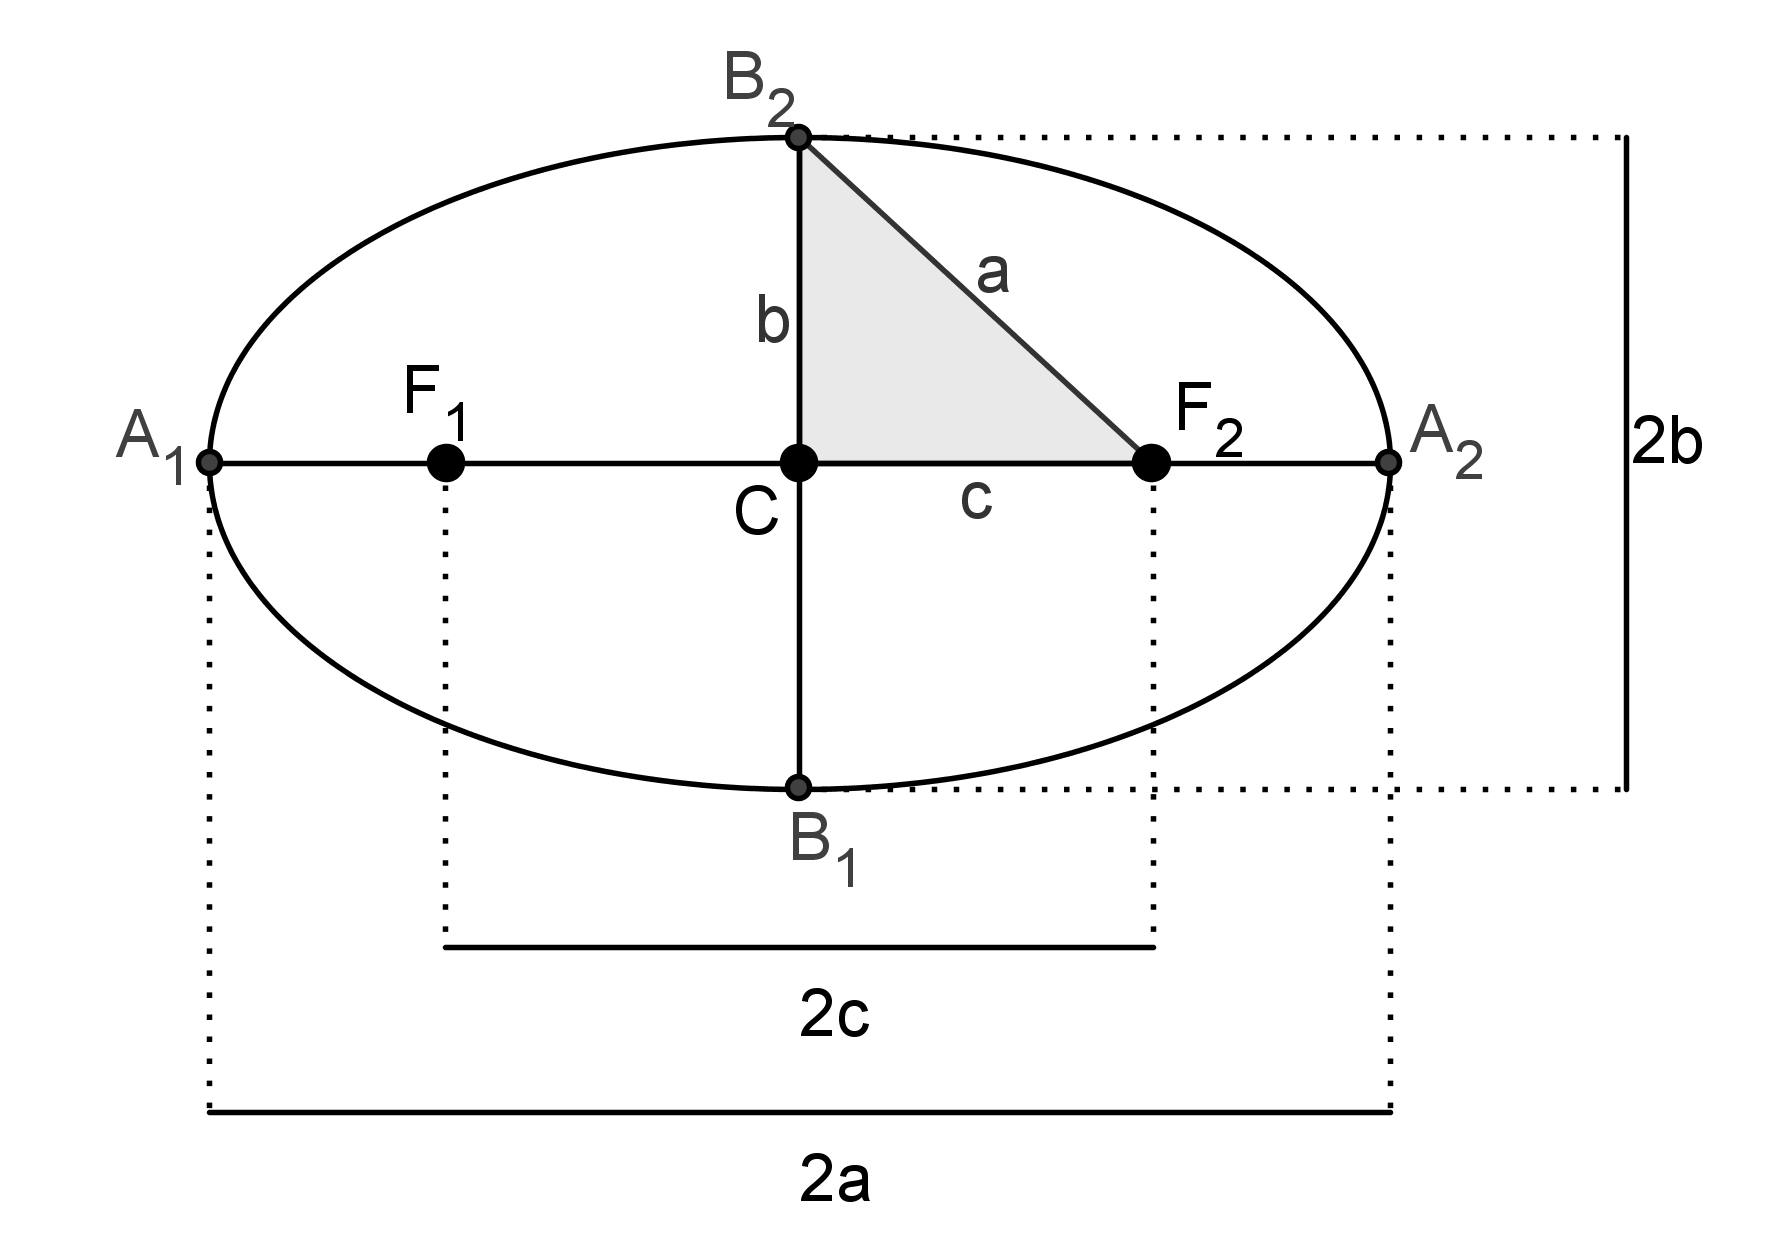
\includegraphics[width=0.45\linewidth]{analitica/imagens/elipse.png}
\caption{Elementos da Elipse}
\label{fig:elipse}
\end{figure}

A elipse possui os seguintes elementos:
\begin{itemize}
  \item \textbf{Focos:} são os pontos $F_1$ e $F_2$.
  \item \textbf{Distância focal:} é a distância $2c$ entre os focos.
  \item \textbf{Centro:} é o ponto médio do segmento $F_1F_2$.
  \item \textbf{Eixo Maior:} é o segmento $A_1A_2$ de comprimento $2a$. O eixo maior é o segmento que contém os focos.
  \item \textbf{Eixo Menor:} é o segmento $B_1B_2$ de comprimento $2b$. O eixo menor é perpendicular ao segmento $A_1A_2$ no centro $C$.
  \item \textbf{Excentricidade:} é o número real $\displaystyle e=\frac{c}{a}$. Indica o ``grau de achatamento'' da elipse. Excentricidade perto de 0 indicam elipses quase circulares, enquanto que excentricidade perto de 1 indica elipse bastante achatada ou alongada.
\end{itemize}

Observe que: $$a^2=b^2+c^2$$ e esta igualdade mostra que $b$ e $c$ são menores do que $a$.

\subsection{Equações reduzidas da elipse}

Considere um sistema cartesiano, e adotemos os focos da elipse sobre o eixo $Ox$. Desta forma, use $F_1(c, 0)$, $F_2(-c,0)$, a distância entre os focos $2c$, a constante da definição $2a$ e utilize a fórmula da distância para deduzir a equação reduzida da elipse.
\begin{eqnarray*}
d(P, F_1)+d(P, F_2)&=&2a \\
\sqrt{(x+c)^2+y^2} + \sqrt{(x-c)^2+y^2}& = & 2a  \\
&\vdots &\\
(a^2-c^2)x^2+a^2y^2&=&a^2b^2 \\
b^2x^2+a^2y^2&=&a^2b^2 \\
\frac{x^2}{a^2}+\frac{y^2}{b^2}& =& 1
\end{eqnarray*}
que é a \textit{equação reduzida} para esta situação.

\begin{figure}[H]
\centering
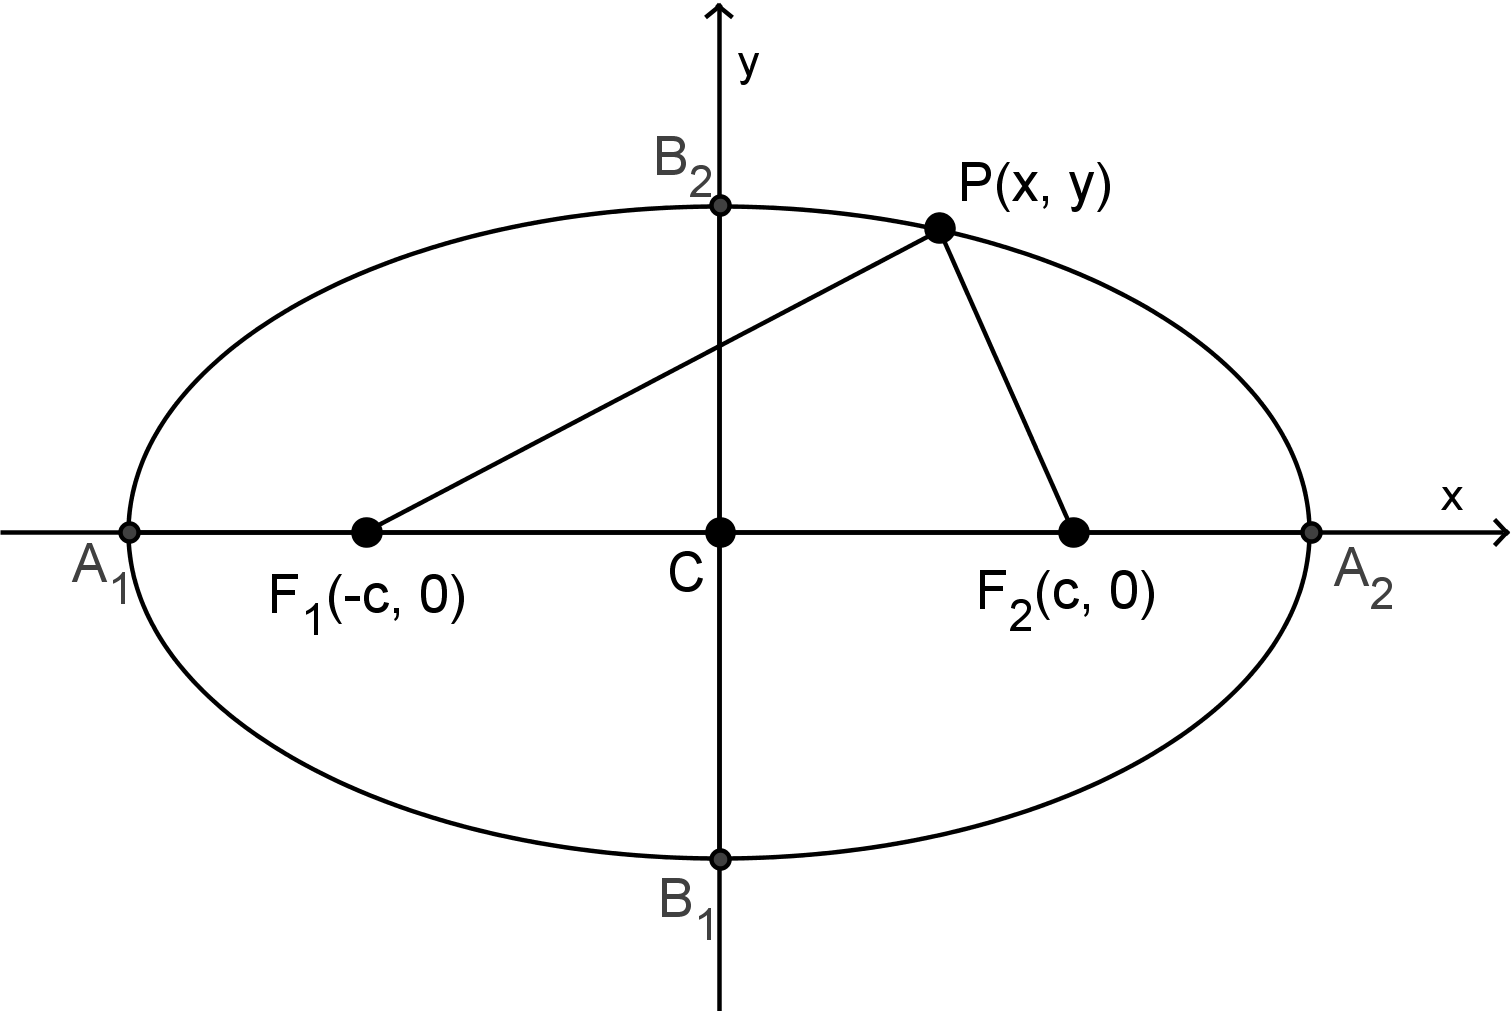
\includegraphics[width=0.45\linewidth]{analitica/imagens/elipseh1.png}
\caption{Elipse }
\label{fig:elipseh1}
\end{figure}

Para o caso do eixo maior sobre o eixo $Oy$, teremos uma situação análoga, com a seguinte \textit{equação reduzida}:

$$\frac{x^2}{b^2}+\frac{y^2}{a^2}=1$$

Para identificar o eixo maior da elipse, basta verificar onde está o maior denominador. Por exemplo, para a elipse $\displaystyle \frac{x^2}{16}+\frac{y^2}{9}=1$, temos que o eixo maior será $Ox$, pois o termo $x^2$ possui o maior denominador.

Para um caso mais geral, considerando o centro da elipse em $C(h, k)$, a equação da elipse será dada por $$\frac{\left(x-h\right)^2}{a^2}+\frac{\left(y-k\right)^2}{b^2}=1$$ que possui o eixo maior paralelo a $Ox$, ou $$\frac{\left(x-h\right)^2}{b^2}+\frac{\left(y-k\right)^2}{a^2}=1$$ que possui eixo maior paralelo ao eixo $Oy$.

\section{Hipérbole}

Hipérbole é o conjunto de todos os pontos de um plano cuja diferença das distâncias a dois pontos fixos $F_1$ e $F_2$ desse plano é constante.

Consideremos no plano dois pontos distintos $F_1$ e $F_2$, tal que a distância $d(F_1, F_2)=2c$, e um número real positivo $a$, de modo que $a<c$.

Seja $P(x, y)$ um ponto do plano, $P$ pertence à hipérbole se, e somente se,

$$|d(P, F_1)-d(P, F_2)|=2a$$

Ou, seja, a hipérbole é uma curva com dois ramos, e desta forma um ponto $P$ pertence à hipérbole se, e somente se
$$d(P, F_1)-d(P, F_2)=\pm 2a$$

\begin{figure}[H]
\begin{minipage}[b]{0.45\linewidth}
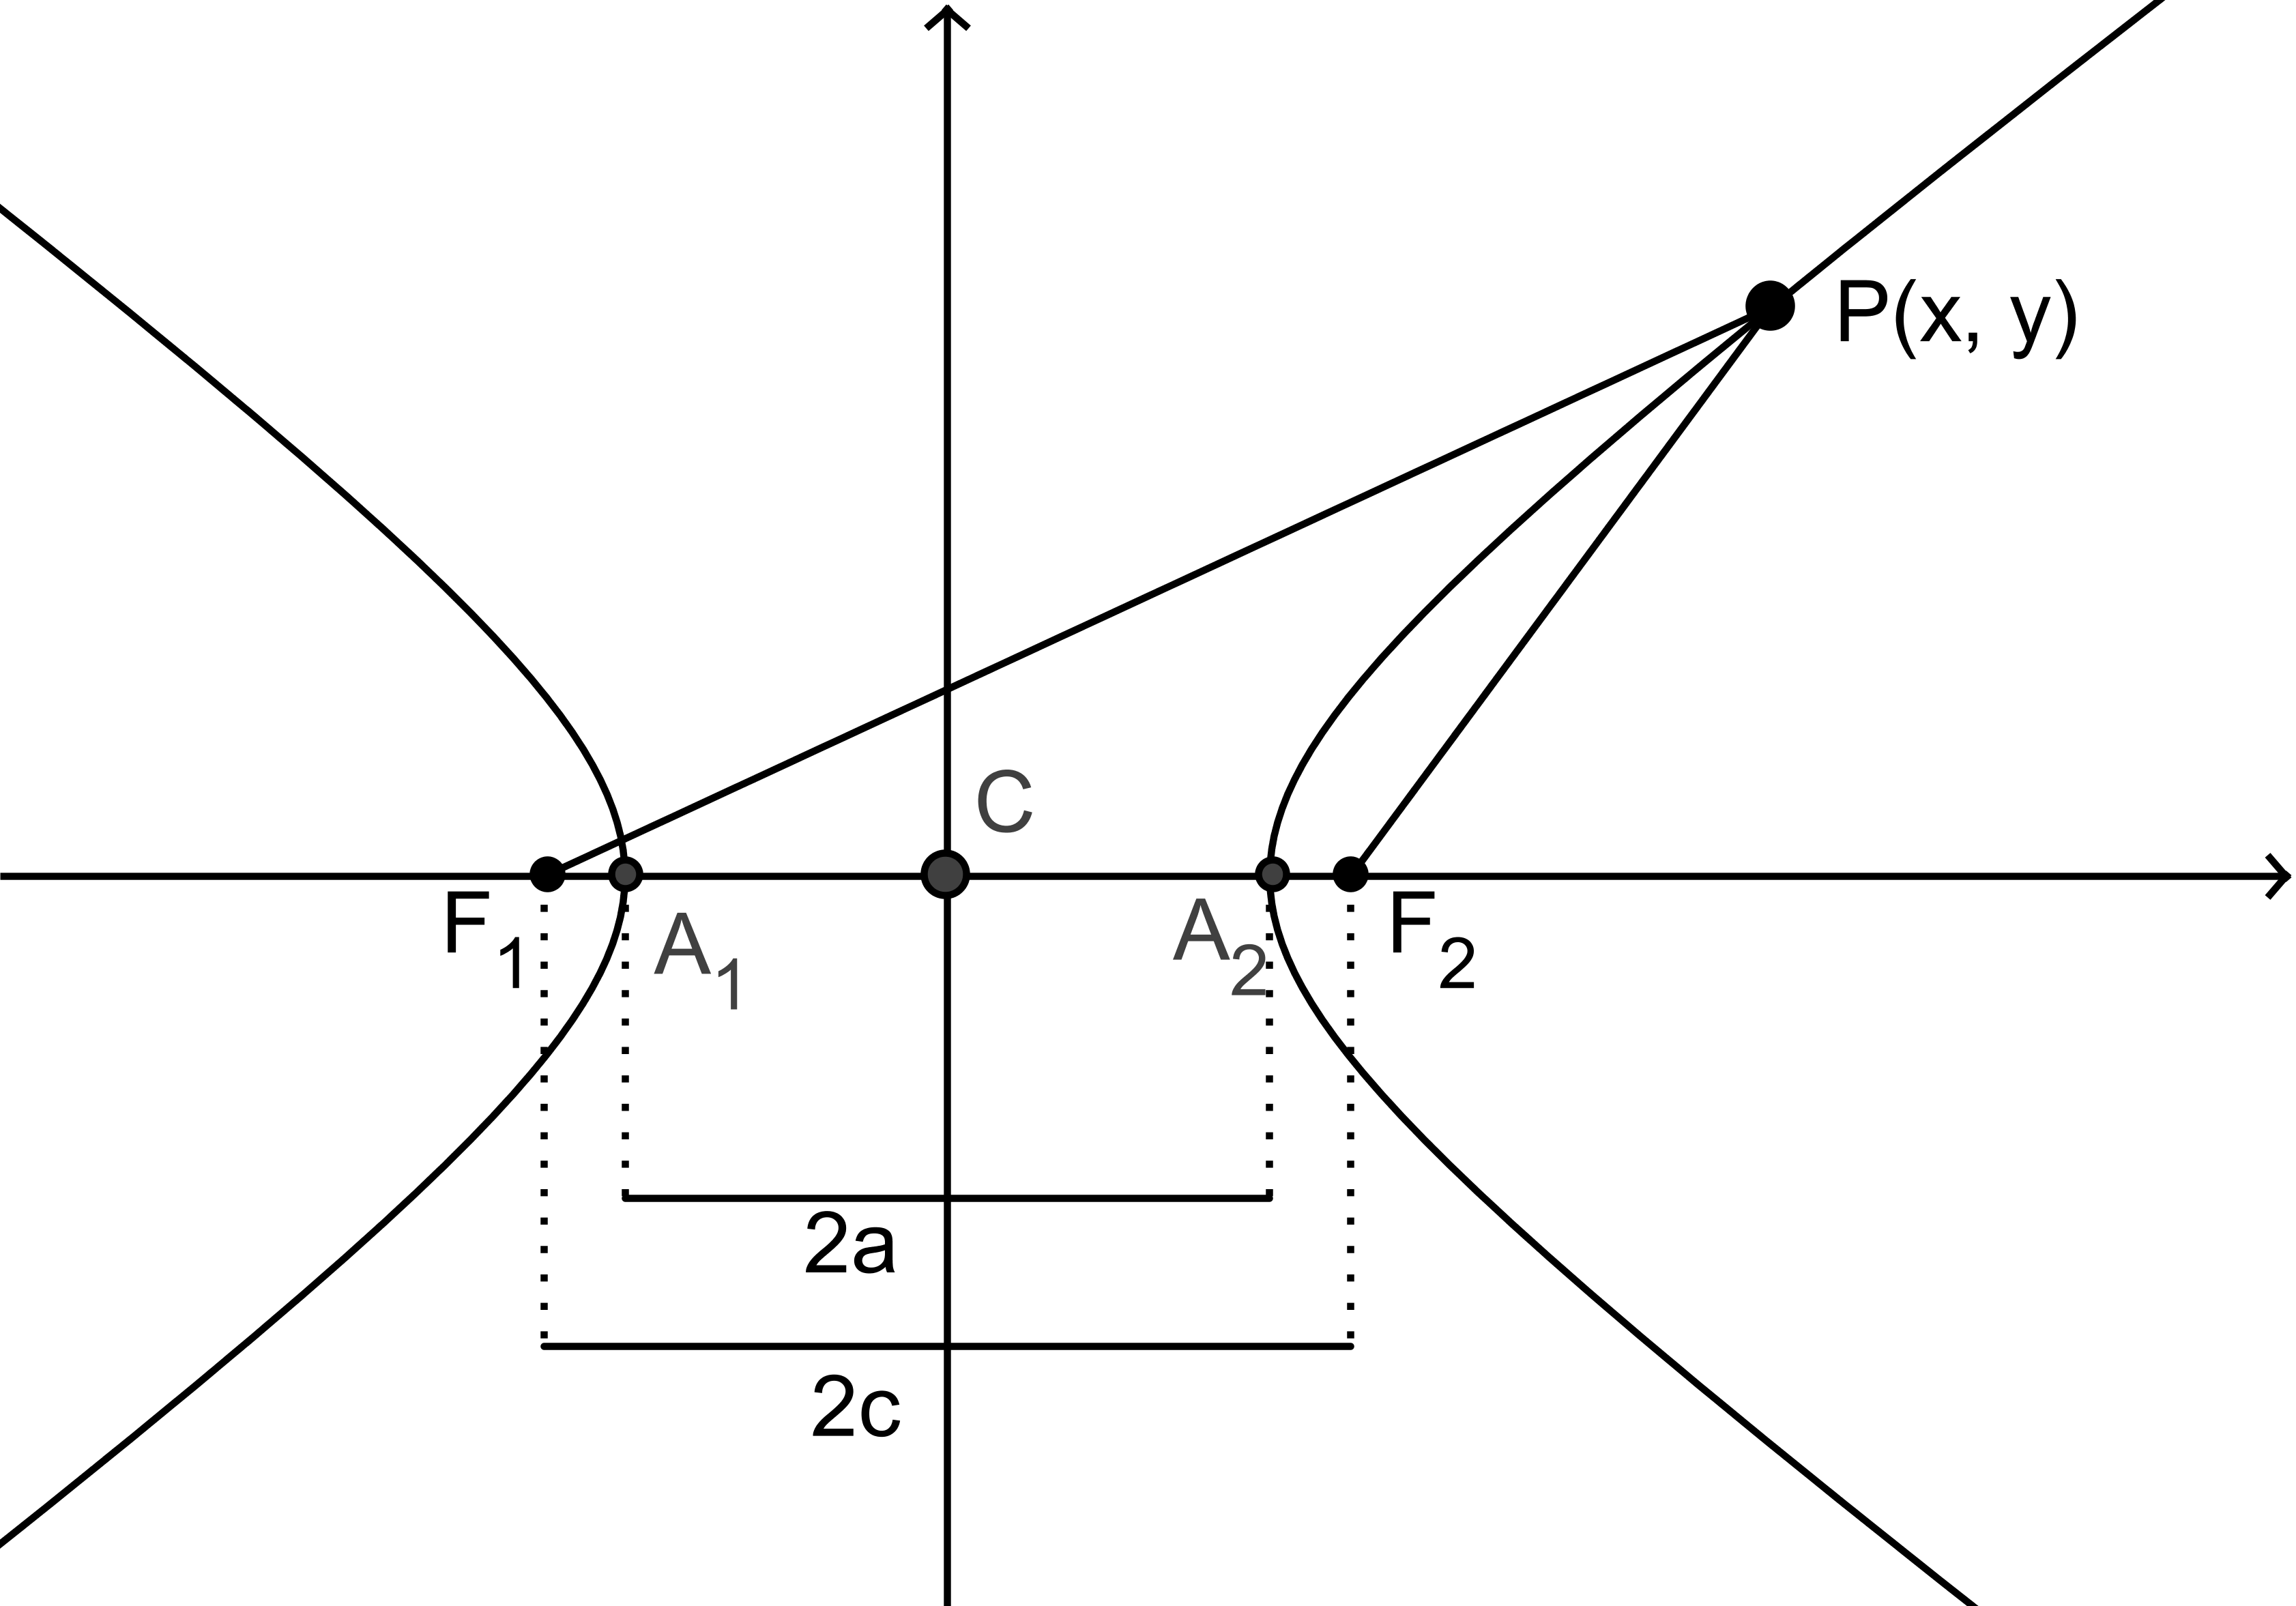
\includegraphics[width=\linewidth]{analitica/imagens/hiperboleh.png}
\caption{Hipérbole}
\label{fig:hiperboel}
\end{minipage} \hfill
\begin{minipage}[b]{0.45\linewidth}
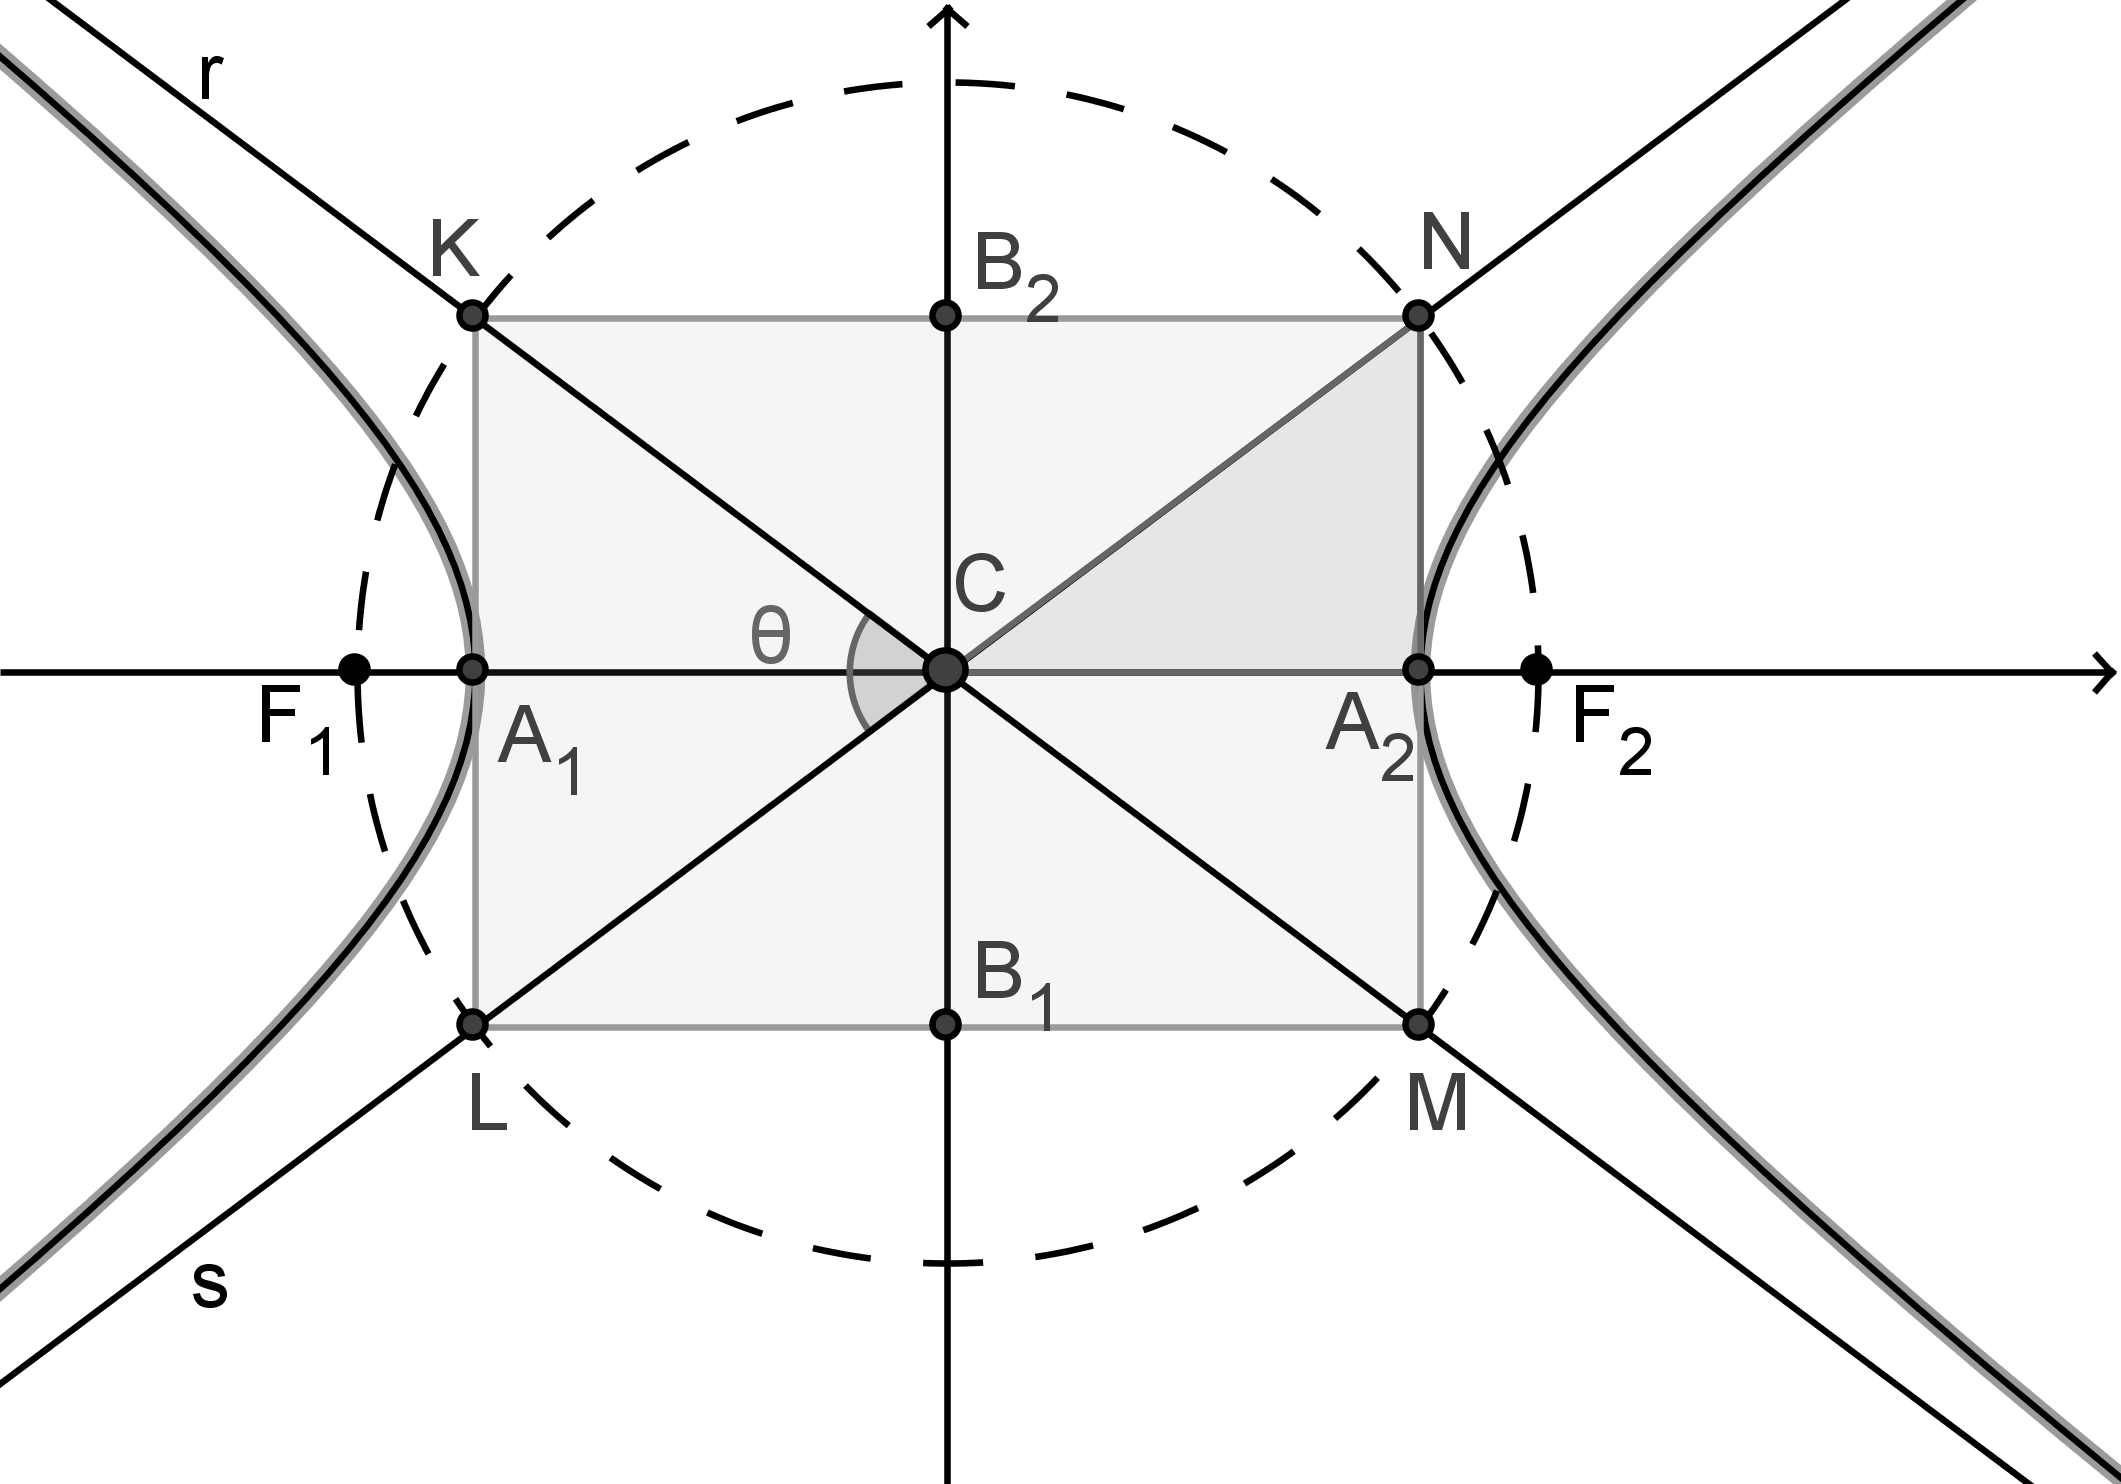
\includegraphics[width=\linewidth]{analitica/imagens/hiperboleh2.png}
\caption{Hipérbole com assíntotas}
\label{fig:hiperbole2}
\end{minipage}
\end{figure}

A hipérbole possui os seguintes elementos:
\begin{itemize}
  \item \textbf{Focos:} são os pontos $F_1$ e $F_2$.
  \item \textbf{Distância focal:} é a distância $2c$ entre os focos.
  \item \textbf{Centro:} é o ponto médio do segmento $F_1F_2$.
  \item \textbf{Eixo real ou transverso:} é o segmento $A_1A_2$ de comprimento $2a$.
  \item \textbf{Eixo imaginário ou não-transverso:} é o segmento $B_1B_2$ de comprimento $2b$. O eixo imaginário é perpendicular ao segmento $A_1A_2$ no centro $C$.
  \item \textbf{Excentricidade:} é o número real $\displaystyle e=\frac{c}{a}$. A excentricidade da hipérbole está relacionada com sua ``abertura'', ou com o ângulo $\theta$ indicado.
\end{itemize}
Observe que: $$c^2=a^2+b^2$$ e esta igualdade mostra que $a$ e $b$ são menores do que $c$.

\subsection{Equações reduzidas da hipérbole}

Considere um sistema cartesiano, e adotemos os focos da hipérbole sobre o eixo $Ox$. Desta forma, use $F_1(-c, 0)$, $F_2(c,0)$, a distância entre os focos $2c$, a constante da definição $2a$ e utilize a fórmula da distância para deduzir a equação reduzida da elipse.
\begin{eqnarray*}
|d(P, F_1)-d(P, F_2)|&=&2a \\
\left| \sqrt{(x+c)^2+y^2} - \sqrt{(x-c)^2+y^2}\right| & = & 2a  \\
&\vdots &\\
\frac{x^2}{a^2}-\frac{y^2}{b^2}& =& 1
\end{eqnarray*}
que é a \textit{equação reduzida} para esta situação.

\begin{figure}[H]
\centering
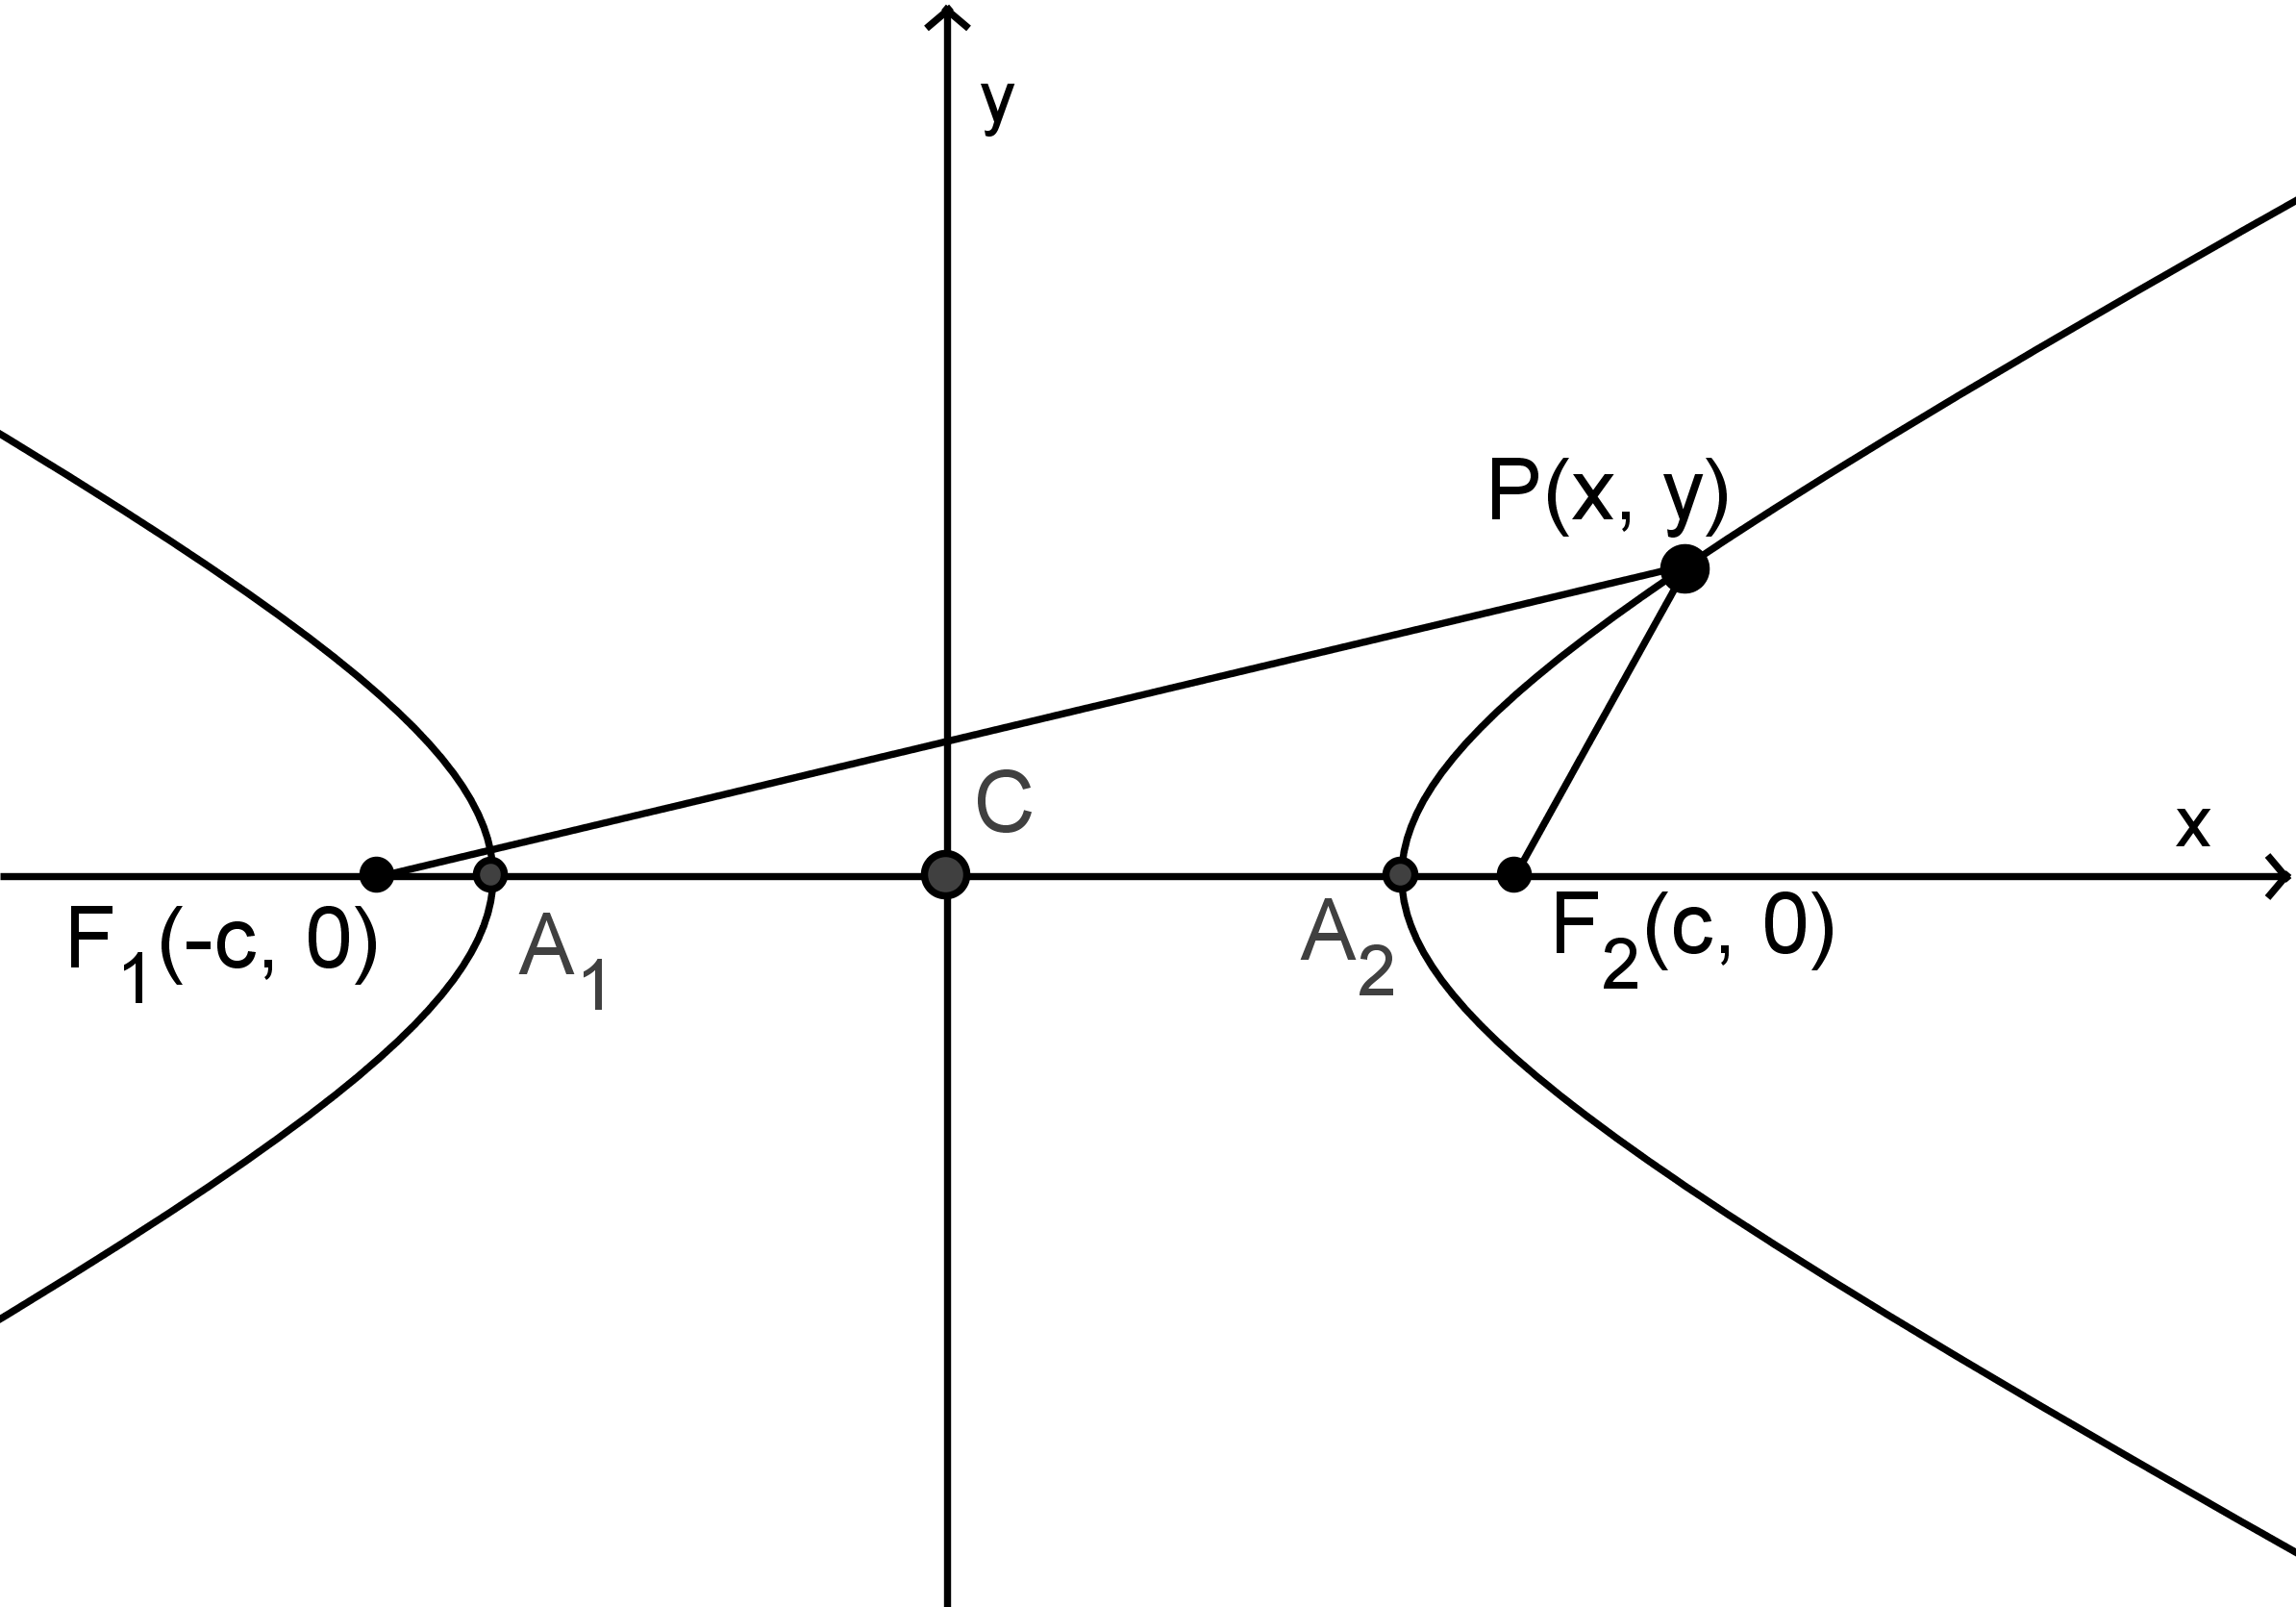
\includegraphics[width=0.45\linewidth]{analitica/imagens/hiperboleh3.png}
\caption{Hipérbole}
\label{fig:hiperh3}
\end{figure}

Para o caso do eixo real sobre o eixo $Oy$, teremos uma situação análoga, com a seguinte \textit{equação reduzida}:

$$\frac{y^2}{a^2}-\frac{x^2}{b^2}=1$$

\begin{figure}[H]
\centering
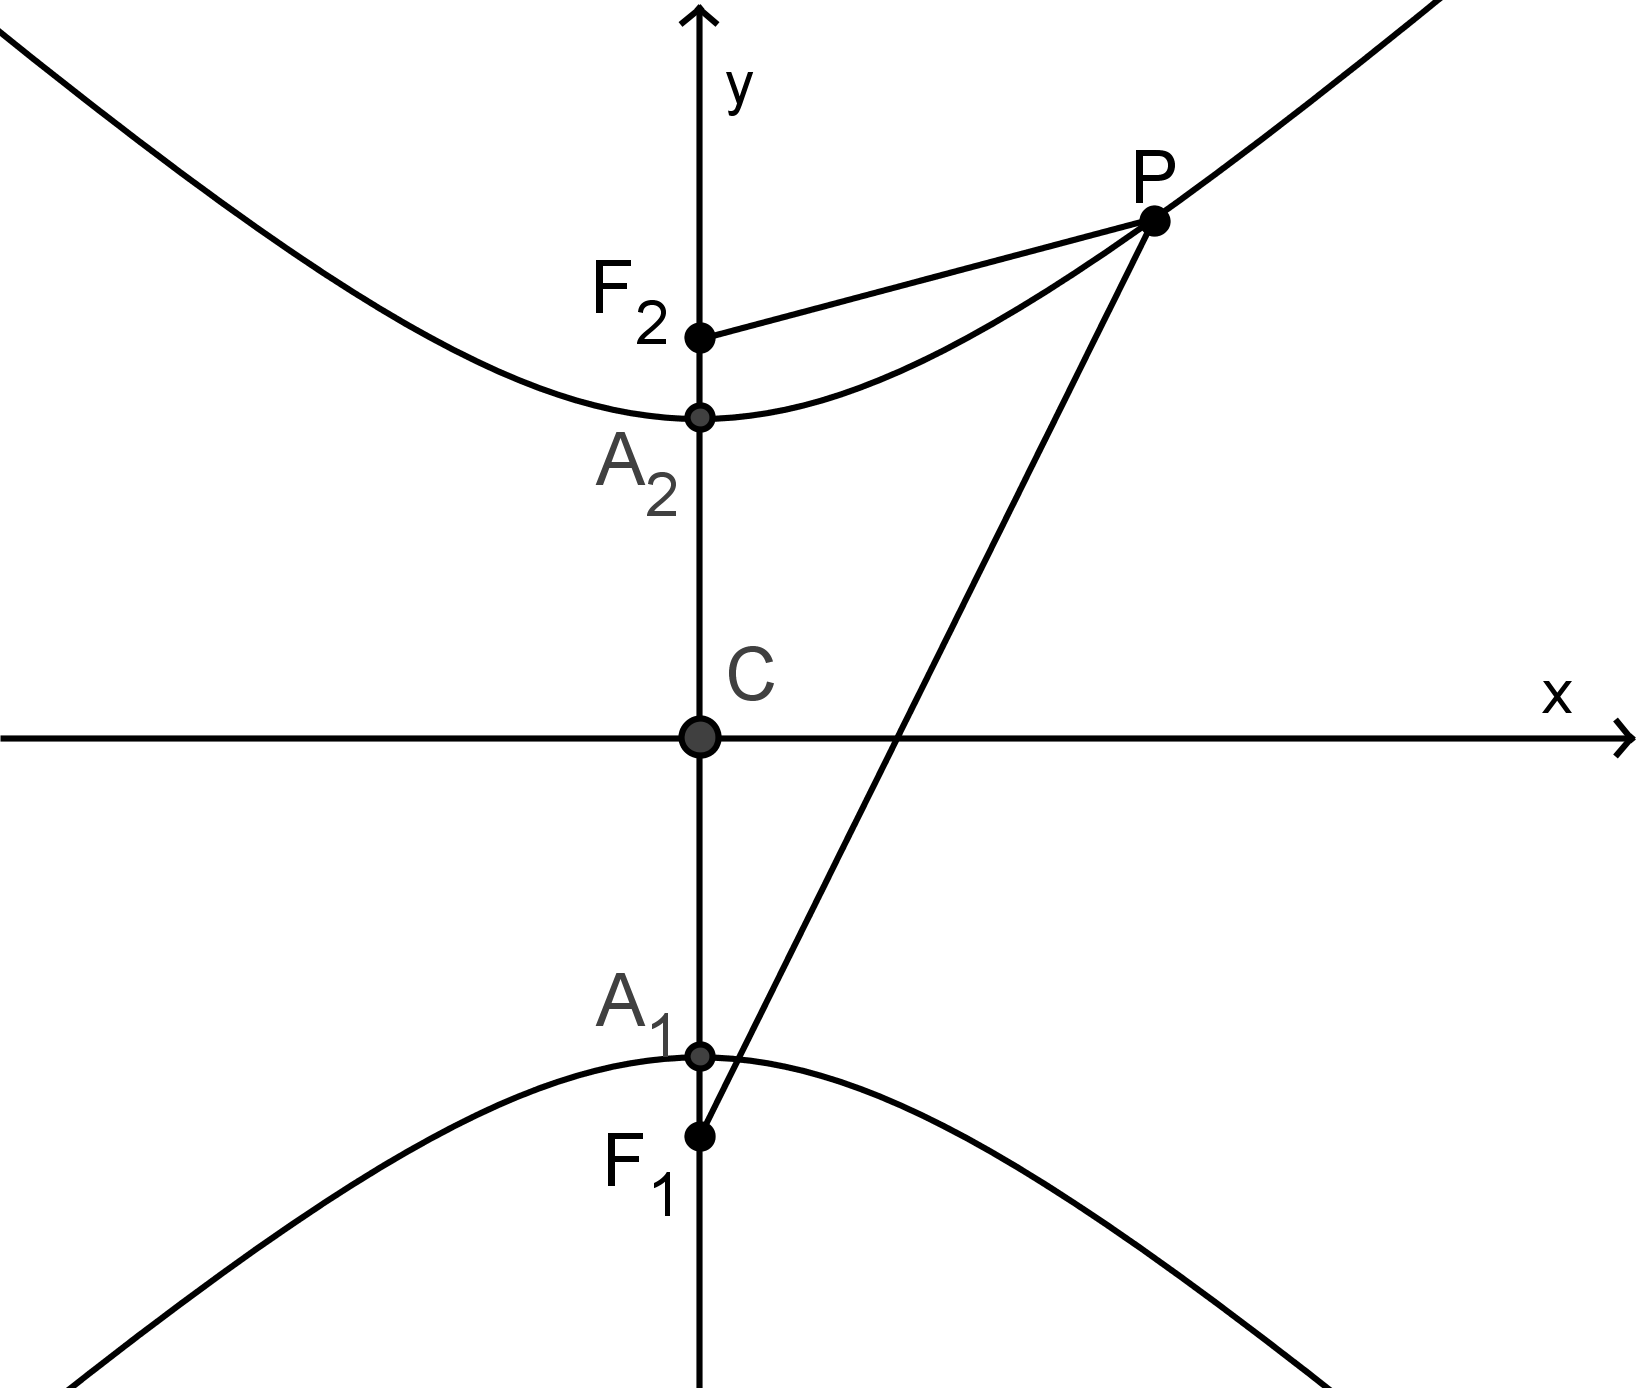
\includegraphics[width=0.35\linewidth]{analitica/imagens/hiperbolev.png}
\caption{Hipérbole com eixo real sobre $Oy$}
\label{fig:hiperv}
\end{figure}

\vspace{1cm}

Para um caso mais geral, considerando o centro da hipérbole em $C(h, k)$, a equação da hipérbole será dada por $$\frac{\left(x-h\right)^2}{a^2}-\frac{\left(y-k\right)^2}{b^2}=1$$ que possui o eixo real paralelo a $Ox$, ou $$\frac{\left(y-k\right)^2}{a^2}-\frac{\left(x-h\right)^2}{b^2}=1$$ que possui eixo real paralelo ao eixo $Oy$.
\part{Geometria Euclidiana}
	\parttoc
\chapter{Noções Primitivas}
Para iniciar o estudo da geometria euclidiana, iremos nos basear em proposições e entes primitivos. São estes o ponto, a reta e o plano. \par %DESENHO de ponto, reta e plano%
No livro \textit{Os Elementos}, Euclides descreve estes entes através de suas dimensões. Ponto é aquilo que não tem parte, nem dimensão. Reta é aquilo que tem comprimento sem largura. Plano é aquilo que tem comprimento e largura. %conferir as citações.
Aqui, usaremos letras latinas maiúsculas para pontos, letras latinas minúsculas para retas e letras gregas para planos. \par 
Além dos entes acima, tomaremos os seguintes postulados sem demonstrações.

\begin{post}[Postulado da Existência]
Em uma reta, bem como fora dela, existem infinitos pontos.
Num plano, há infinitos pontos.
\end{post}
\begin{post}[Postulado da Determinação da Reta]
Dois pontos distintos determinam uma única reta que passa por eles.
\end{post}
\begin{df}
Pontos \emph{colineares} são pontos que pertencem a uma mesma reta.
\end{df}
\begin{post}[Postulado da Determinação do Plano]
Três pontos não colineares determinam um único plano que passa por eles.
\end{post}
\begin{post}[Postulado da Inclusão]
Se uma reta tem dois pontos distintos em um plano, então esta reta está contida nesse mesmo plano.
\end{post}
\begin{df}
Pontos \emph{coplanares} são pontos que pertencem a um mesmo plano.
\end{df}
\begin{df}
Duas retas são ditas \emph{concorrentes} se, e somente se, elas tem um único ponto em comum.
\end{df}

\section{Retas}
\blindtext %texto
\subsection{Segmentos de Reta}
Para definirmos um segmento, necessitamos da noção de estar entre. Esta noção segue os seguintes axiomas: \par 
\begin{itemize}
\item Se $P$ está entre $A$ e $B$, então, $A$, $B$ e $P$ são colineares.
\item Se $P$ está entre $A$ e $B$, então, $A$, $B$ e $P$ são distintos dois a dois.
\item Se $P$ está entre $A$ e $B$, então, $A$ não está entre $P$ e $B$, nem $B$ está entre $A$ e $P$.
\item Quaisquer que sejam os pontos $A$ e $B$, se $A \neq B$, então existe $P$ tal que $P$ está entre $A$ e $B$.
\end{itemize}
\begin{df}
Dados $A$ e $B$ distintos, o segmento $\overline{AB}$ é o conjunto dos pontos que estão entre $A$ e $B$.
\end{df}
	\subsubsection{Relações entre Segmentos}
    \paragraph{Segmentos Consecutivos}
    \begin{df}
    Dois segmentos de reta são \emph{consecutivos} se, e somente se, a extremidade de um deles é também extremidade do outro. \end{df}
    \paragraph{Segmentos Colineares}
    \begin{df}
    Dois segmentos de reta são \emph{colineares} se, e somente se, estão contidos em uma mesma reta. \end{df}
    \paragraph{Segmentos Adjacentes}
    \begin{df}
    Dois segmentos de reta consecutivos e colineares são ditos \emph{adjacentes} se, e somente se, a intersecção entre os segmentos for a extremidade compartilhada. \end{df}
    \paragraph{Congruência de Segmentos}
    A relação de congruência, denotada por $\overline{AB} \equiv \overline{CD}$ é uma noção primitiva que satisfaz os seguintes postulados:
    \begin{itemize}
    \item \textbf{Reflexiva}: todo segmento é congruente a si mesmo, ou seja, $\overline{AB} \equiv \overline{AB}$.
    \item \textbf{Simétrica}: se $\overline{AB} \equiv \overline{CD}$, então $\overline{CD} \equiv \overline{AB}$
    \item \textbf{Transitiva}: se $\overline{AB} \equiv \overline{CD}$ e $\overline{CD} \equiv \overline{EF}$, então $\overline{AB} \equiv \overline{EF}$.
    \end{itemize}
\subsection{Semirreta}
\begin{df}
A semirreta $\overrightarrow{AB}$, com origem em $A$ que passa por $B$, é definida como o conjunto de pontos do segmento $\overline{AB}$ unido dos pontos $X$ tais que $B$ está entre $A$ e $X$. Assim, a semirreta se prolonga infinitamente em um sentido.\par 
\end{df}
\paragraph{Semirreta Oposta} Temos, também, a semirreta oposta a $AB$, o conjunto dos pontos $X$ tais que $A$ está entre $X$ e $B$.
Assim, dados dois pontos $A$ e $B$ distintos, temos:
\begin{itemize}
\item a reta $AB$;
\item o segmento $\overline{AB}$
\item a semirreta $\overrightarrow{AB}$
\item a semirreta oposta a $\overrightarrow{AB}$
\item a semirreta $\overrightarrow{BA}$
\item a semirreta oposta a $\overrightarrow{BA}$
\end{itemize}

\subsubsection{Transporte de Segmentos}
\begin{post}[Postulado do Transporte de Segmentos]
Dados um segmento $\overline{AB}$ e uma semirreta de origem $A'$, existe sobre esta semirreta um único ponto $B'$ tal que $\overline{A'B'}$ seja congruente a $\overline{AB}$.
\end{post}
\paragraph{Comparação de Segmentos} Dados dois segmentos $\overline{AB}$ e $\overline{CD}$, pelo postulado do transporte podemos obter um ponto $P$ na semirreta $\overrightarrow{AB}$, tal que $\overline{AP} \equiv \overline{CD}$. Assim, temos três situações:
\begin{itemize}
\item se $P$ está entre $A$ e $B$, então $\overline{AB} > \overline{CD}$
\item se $B$ está entre $P$ e $A$, $\overline{AB} < \overline{CD}$
\item se $P = B$, $\overline{AB} \equiv \overline{CD}$
\end{itemize}
\paragraph{Soma de Segmentos} Dados dois segmentos $\overline{AB}$ e $\overline{CD}$ e tomando uma semirreta qualquer de origem $R$, na qual estão os segmentos adjacentes $\overline{RS}$ e $\overline{ST}$ tais que $\overline{RS} \equiv \overline{AB}$ e $\overline{ST} \equiv \overline{CD}$, temos que o segmento $\overline{RT}$ é a soma de $\overline{AB}$ e $\overline{CD}$.\\
Dizemos que o segmento $\overline{RS}$ que é soma de $n$ segmentos congruentes a $\overline{AB}$ é múltiplo de $\overline{AB}$ segundo $n$, ou seja, $\overline{RS}=n \cdot \overline{AB}$.
\paragraph{Ponto Médio} \begin{df}
O ponto $M$ de um segmento $\overline{AB}$ é dito ponto médio de $\overline{AB}$ se, e somente se, $M \in \overline{AB}$ e $\overline{AM} \equiv \overline{MB}$.
\begin{proof}[Unicidade do Ponto Médio]
Suponhamos $X$ e $Y$ distintos, pontos médios de $\overline{AB}$. Assim, teríamos: \[\overline{AX} \equiv \overline{XB} \textrm{ e } \overline{AY} \equiv \overline{YB}\]
Portanto, podemos afirmar que
\[ \left. \begin{array}{ll}
			X\textrm{ está entre }A\textrm{ e }Y &\Rightarrow \overline{AY} > \overline{AX}\\
            &\textrm{e}\\
			Y\textrm{está entre }X\textrm{ e }B &\Rightarrow \overline{XB}>\overline{YB} \end{array} \right\} \Rightarrow \overline{AY}>\overline{AX}\equiv \overline{XB}>\overline{YB}\]
o que é absurdo, pois $\overline{AY} \equiv \overline{YB}$, ou então
\[ \left. \begin{array}{ll}
			Y\textrm{ está entre }A\textrm{ e }X &\Rightarrow \overline{AX} > \overline{AY}\\
			&\textrm{e}\\
			X\textrm{ está entre }Y\textrm{ e }B &\Rightarrow \overline{YB} > \overline{XB}
		\end{array} \right\} \Rightarrow \overline{AX}>\overline{YA}\equiv \overline{YB} > \overline{XB}\]
        o que é absurdo, pois $\overline{AX}\equiv \overline{XB}$. Portanto, o ponto médio é único.
\end{proof}
\end{df}

\paragraph{Medida do Segmento} A medida de um segmento $\overline{AB}$ é denotada por $m(\overline{AB})$ ou simplesmente $AB$. A medida de um segmento não nulo é um número real positivo associado ao segmento tal que:
\begin{itemize}
\item Segmentos congruentes possuem medidas iguais.
\item Se um segmento é maior do que outro, sua medida é maior do que a medida do outro.
\item A medida de um segmento soma é a soma das medidas dos segmentos parcelas.
\end{itemize}
\subparagraph{Distância Geométrica} A distância geométrica entre dois pontos $A$ e $B$ é o segmento $\overline{AB}$ ou qualquer segmento congruente a $\overline{AB}$.
\subparagraph{Distância Métrica} A distância métrica entre dois pontos $A$ e $B$ é a medida do segmento $\overline{AB}$. Esta medida é medida através de uma unidade, como o metro, o centímetro ou qualquer outra unidade definida. \\ 
Se $A+B$, temos que a distância geométrica é nula, e a distância métrica é igual a zero.

\subsection{Ângulos}
\begin{df}
\emph{Ângulo} é o nome dado a união de duas semirretas $\overrightarrow{OA}$ e $\overrightarrow{OB}$ de mesma origem ``$O$'', chamada \emph{vértice}. Denotamos este ângulo por $A\hat{O}B$.
\end{df}
Se $\overrightarrow{OA}=\overrightarrow{OB}$, chamamos este ângulo de \emph{ângulo nulo}. Se $\overrightarrow{OA}$ é oposta a $\overrightarrow{OB}$, chamamos este ângulo de \emph{ângulo raso}.
\subsubsection{Regiões Convexas}
\begin{df}
Um conjunto de pontos $\Phi$ é dito \emph{convexo} se, e somente se, para quaisquer pontos $A,B \in \Phi$, $\overline{AB} \subset \Phi$.
Se uma região não é convexa, ela é chamada de \emph{região côncava}.
\end{df}
\begin{post}[Postulado da separação dos pontos de um plano]
Uma reta $r$ de um plano $\alpha$ separa este plano em dois conjuntos de pontos $\alpha'$ e $\alpha''$ tais que:
\begin{enumerate}[i)]
\item $\alpha' \cap \alpha'' = \emptyset$
\item $\alpha'$ e $\alpha''$ são convexos
\item $A \in \alpha', B \in \alpha''$,  $\overline{AB} \cap r \neq \emptyset $
\end{enumerate}
\end{post}
\begin{df}
Chamamos as regiões $\alpha'$ e $\alpha''$ de \emph{semiplanos abertos}. $\alpha' \cup r$ e $\alpha'' \cup r$ são chamados \emph{semiplanos}, onde $r$ é dita a \emph{origem} de cada um dos semiplanos. $\alpha'$ e $\alpha'$ são ditos \emph{semiplanos opostos}.
\end{df}
\paragraph{Interior do Ângulo} O interior de $A\hat{O}B$ pertencente ao plano $\Sigma$ é a intersecção dos semiplanos abertos:
\begin{itemize}
\item $\alpha_1$ com origem na reta $\overleftrightarrow{OA}$ que contém o ponto $B$. 
\item $\beta_1$ com origem na reta $\overleftrightarrow{OB}$ que contém o ponto $A$.
\end{itemize}
O interior de um ângulo é convexo, e a união de um ângulo com seu interior é chamada \emph{setor angular}.
\paragraph{Exterior do Ângulo} O exterior de $A\hat{O}B$ é o conjunto dos pontos pertencentes ao plano $\Sigma$ que não pertencem ao ângulo ou ao seu interior. Assim, é a união de dois semiplanos $\alpha_2$ e $\beta_2$, opostos a $\alpha_1$ e $\beta_1$, respectivamente. O exterior de um ângulo é côncavo.
\subsubsection{Relações entre Ângulos}
	\paragraph{Ângulos Consecutivos}
    Dois ângulos são ditos consecutivos se possuem um lado compartilhado.
    \begin{df}
Dois ângulos são \emph{consecutivos} se, e somente se, um lado de um deles é também lado do outro.
\end{df}
    \paragraph{Ângulos Adjacentes}
    Dois ângulos consecutivos são ditos adjacentes se não possuem pontos interiores em comum.
    \begin{df}
Dois ângulos consecutivos são \emph{adjacentes} se, e somente se\[{Interior}_{A\hat{O}B} \cap {Interior}_{B\hat{O}C} = \emptyset\]
\end{df}
    \paragraph{Ângulos opostos pelo Vértice}
    %o fato de serem congruentes só pode ser provado com o suplementar adjacente. então colocar lá
    \paragraph{Ângulos Congruentes}
\subsection{Transporte de Ângulos}
	\paragraph{Comparação de Ângulos}
    \paragraph{Soma de Ângulos}
    \paragraph{Bissetriz de um Ângulo}
\subsection{Medidas de Ângulos}
	\paragraph{Ângulo Suplementar Adjacente}
    Dado um ângulo $A\hat{O}B$, a semirreta $\overrightarrow{OC}$ oposta a $\overrightarrow{OA}$ e a semirreta $\overrightarrow{OB}$, dizemos que $B\hat{O}C$ é \emph{suplementar adjacente} a $A\hat{O}B$. 
    \begin{prop}
Dois ângulos opostos pelo vértice são congruentes.
\begin{proof}
Tomemos os ângulos opostos pelo vértice $\angle AOB$ e $\angle COD$. Assim, temos que o ângulo $\angle BOC$ é suplementar adjacente de ambos $\angle AOB$ e $\angle COD$.\\
Assim, temos que $\angle AOB \equiv \angle COD$.
\end{proof}
\end{prop}
    \paragraph{Ângulo Reto} \emph{Ângulo reto} é todo ângulo congruente ao seu suplementar adjacente.
    \paragraph{Ângulo Agudo} Um ângulo \emph{menor do que} um ângulo reto é chamado \emph{ângulo agudo}.
    \paragraph{Ângulo Obtuso} Um ângulo \emph{maior do que} um ângulo reto é chamado \emph{ângulo obtuso}.
    \paragraph{Medida de um Ângulo} 
    \subparagraph{Unidades de Medida} 
    \paragraph{Ângulos Complementares} 
    \paragraph{Ângulos Suplementares} 
\chapter{Triângulos}
A partir de três pontos não colineares, conseguimos definir segmentos cuja intersecção, dois a dois, são suas extremidades. A partir da união destes segmentos, definimos triângulos.
\begin{df}
Dados três pontos $A,B,C$ não colineares, denominamos a união dos segmentos $\overline{AB}, \overline{BC}, \overline{CA}$ de triângulo $ABC$.
\[\textrm{triângulo } ABC = \triangle ABC = \overline{AB} \cup \overline{BC} \cup \overline{CA}\]
\end{df}
As extremidades dos segmentos que formam o triângulo são chamadas \emph{vértices}. Os ângulos $\angle ABC$, $\angle BCA$ e $\angle CAB$ são ditos \emph{opostos} aos segmentos $\overline{AC}$, $\overline{AB}$, $\overline{CB}$ (enquanto os segmentos são chamados \emph{lados}). Usualmente utilizamos a letra do vértice oposto para a medida de um segmento, ou seja, $c$ é a medida do segmento $\overline{AB}$.

\Blindtext
\part{Lógica}
	\parttoc
\chapter{Proposições}
\begin{df}
Proposição lógica é uma sentença declarativa sem variável com valor lógico definido (verdadeiro ou falso). O valor lógico de uma proposição $p$ é denotado por $\mathcal{V}(p)$.
\end{df}
\begin{exemplo}
\[p:\text{ O Brasil é um país da América do Sul}\]
\[q:\ 3 \in \mathbb{N}\]
\[r: 9 \ge \sqrt{99} \]
\[\mathcal{V}(p)\Leftrightarrow V\]
\end{exemplo}

Cada proposição possui um valor lógico próprio, que segue certos princípios:
\begin{itemize}
	\item \textbf{Princípio da Identidade:} uma proposição falsa é falsa, e uma proposição verdadeira é verdadeira.
	\item \textbf{Princípio do Terceiro Excluído:} uma proposição lógica é verdadeira ou falsa, não existindo um terceiro valor lógico. 
	\item \textbf{Princípio da Não-Contradição:} uma proposição lógica verdadeira não é falsa, e uma proposição falsa não é verdadeira, ou seja, uma proposição não pode ser falsa e verdadeira simultaneamente.
\end{itemize}
Proposições lógicas podem ser simples ou compostas. Os exemplos acima são proposições simples. Proposições compostas são formadas por duas ou mais proposições simples ligadas por meio de conetivos lógicos.
\begin{exemplo}
\[p \textbf{ e } q: \text{O Brasil é um país da América do Sul \textbf{e }} 3 \in \mathbb{N}\]
\[\textbf{se } r \textbf{ então }q:\text{ \textbf{se} }  9 \ge \sqrt{99} \text{ \textbf{então} } \ 3 \in \mathbb{N}\]
\[\textbf{não } p: \text{O Brasil \textbf{não }é um país da América do Sul}\]
\end{exemplo}

\section{Tabela-Verdade}
Para representar as combinações de valores lógicos de uma ou mais proposições, é comum se utilizar a tabela-verdade. É uma tabela composta por colunas em mesmo número do que as proposições a serem analisadas, e o número de linhas é igual a \(2^n\), sendo n o número de proposições. Isto é facilmente explicado, sabendo que cada proposição possui um valor lógico definido, verdadeiro ou falso.

\begin{table}[H]
\centering
\caption{Tabela Verdade para 2 proposições}
\label{2prop}
\begin{tabular}{c|c} 
\textbf{p} & \textbf{q} \\ \hline
V          & V          \\
V          & F          \\
F          & V          \\
F          & F         
\end{tabular}
\end{table}
\vspace{-0.5cm}
\begin{table}[H]
\centering
\caption{Tabela Verdade para 3 proposições}
\label{3prop}
\begin{tabular}{c|c|c}
\textbf{p}  & \textbf{q} &  \textbf{r} \\ \hline
V          & V          & V          \\
V          & V          & F          \\
V          & F          & V          \\
V          & F          & F          \\
F          & V          & V          \\
F          & V          & F          \\
F          & F          & V          \\
F          & F          & F         
\end{tabular}
\end{table}

\section{Conetivos Lógicos}
Os conetivos ou operadores lógicos são elementos que relacionam ou alteram proposições. São eles:
\subsection*{Negação}
A negação é um operador unário: ela opera apenas sobre o valor da proposição simples. Assim, se a proposição $p$ é verdadeira, sua negação, $\sim p$ é falsa. Se a proposição $p$ é falsa, $\sim p$ é verdadeira. A negação é interpretada como \textit{não ...} ou \textit{não é verdade que ...} .
\begin{table}[H]
\centering
\caption{Negação}
\label{not}
\begin{tabular}{c|c}
\textbf{p} & \textbf{$\sim$ p} \\ \hline
V          & F                 \\
F          & V                
\end{tabular}
\end{table}

\begin{exemplo}
Vamos supor $p: \text{A girafa é um mamífero}.$ $\sim p$, então, seria ``a girafa \textbf{não} é um mamífero.'' Já que o nosso $p$ é verdadeiro ($\mathcal{V}(p) \Leftrightarrow V$), o nosso $\sim p$ é falso ($\mathcal{V}(\sim p) \Leftrightarrow F$).
\end{exemplo}

\subsection*{Conjunção}
A conjunção verifica a existência de uma proposição falsa. Se alguma proposição é falsa, a conjunção será falsa. Se ambas as proposições forem verdadeiras, a conjunção das proposições será verdadeira. A conjunção é interpretada como \textit{``... e ...''} .
\begin{table}[H]
\centering
\caption{Conjunção}
\label{and}
\begin{tabular}{c|c|c}
\textbf{p} & \textbf{q} & \textbf{p $\wedge$ q} \\ \hline
V          & V          & V             \\
V          & F          & F             \\
F          & V          & F             \\
F          & F          & F            
\end{tabular}
\end{table}

\begin{exemplo}
$p:\text{João está com fome}$, $q:\text{Maria está com sede}$. Se João estiver com fome ($\mathcal{V}(p) \Leftrightarrow V$) e Maria estiver com sede ($\mathcal{V}(q) \Leftrightarrow V$), então p $\wedge$ q é verdadeiro ($\mathcal{V}(p \wedge q) \Leftrightarrow V$), pois as duas proposições são verdadeiras . Nos outros casos, como o João pode estar sem fome ($\mathcal{V}(p) \Leftrightarrow F$), ou a Maria estar sem sede ($\mathcal{V}(q) \Leftrightarrow F$), ou os dois estarem simultaneamente sem fome e sede respectivamente, nossa conjunção é falsa ($\mathcal{V}(p \wedge q) \Leftrightarrow F$), pois temos pelo menos uma proposição falsa. 
\end{exemplo}

\subsection*{Disjunção}
A disjunção verifica a existência de uma proposição verdadeira. Se ao menos uma proposição é verdadeira, a disjunção será verdadeira. Se ambas as proposições forem falsas, a disjunção das proposições será falsa. A disjunção é interpretada como \textit{``... ou ...''} .
\begin{table}[H]
\centering
\caption{Disjunção}
\label{or}
\begin{tabular}{c|c|c}
\textbf{p} & \textbf{q} & \textbf{p $\vee$ q} \\ \hline
V          & V          & V             \\
V          & F          & V             \\
F          & V          & V             \\
F          & F          & F            
\end{tabular}
\end{table}
\begin{exemplo}
$p:\text{Maria viajará para a Argentina}$, $q:\text{Maria viajará com João}$. Se Maria viajar para a Argentina ($\mathcal{V}(p) \Leftrightarrow V$) com o João ($\mathcal{V}(q) \Leftrightarrow V$), então Maria viajou para a Argentina ou com o João ($\mathcal{V}(p \vee q) \Leftrightarrow V$). Apenas caso Maria não viaje para a Argentina, nem com o João, ($\mathcal{V}(p \vee q) \Leftrightarrow F$).
\end{exemplo}

\subsection*{Condicional}
O condicional é um operador que gera uma relação de hipótese-tese. Para o condicional ser verdadeiro, devemos verificar a primeira proposição. Caso esta seja verdadeira, devemos analisar a segunda proposição. Caso a primeira seja verdadeira, o valor lógico do condicional será equivalente ao da segunda proposição. Caso a primeira seja falsa, o condicional é verdadeiro (a condição não se aplica). O condicional é interpretado como \textit{``se ... então ...''} .
\begin{table}[H]
\centering
\caption{Condicional}
\label{ifso}
\begin{tabular}{c|c|c}
\textbf{p} & \textbf{q} & \textbf{p $\rightarrow$ q} \\ \hline
V          & V          & V             \\
V          & F          & F             \\
F          & V          & V             \\
F          & F          & V            
\end{tabular}
\end{table}
\begin{exemplo}
$p: \text{João é menor de idade}.$, $\: q: \text{João tem autorização dos pais}$. Caso João seja menor de idade ($\mathcal{V}(p) \Leftrightarrow V$), então ele deverá ter autorização dos pais ($\mathcal{V}(q) \Leftrightarrow V$) para que entre na festa ($\mathcal{V}\left( p \rightarrow q\right) \Leftrightarrow V$). Caso João seja maior de idade ($\mathcal{V}(p) \Leftrightarrow F$), ele não precisará da autorização dos pais, pois tendo ela ou não ele entrará na festa.
\end{exemplo}

\subsection*{Bicondicional}
O bicondicional é um operador que compara o valor lógico das proposições. Se o valor das proposições for equivalente (ambas verdadeiras ou falsas), o bicondicional será verdadeiro. Caso contrário (uma verdadeira e uma falsa), o bicondicional será falso. O bicondicional é interpretado como \textit{``... se e somente se ...''} .
\begin{table}[H]
\centering
\caption{Bicondicional}
\label{ifonlyif}
\begin{tabular}{c|c|c}
\textbf{p} & \textbf{q} & \textbf{p $\leftrightarrow$ q} \\ \hline
V          & V          & V             \\
V          & F          & F             \\
F          & V          & F             \\
F          & F          & V            
\end{tabular}
\end{table}
\begin{exemplo}
$p: \text{Taís está triste}$, $q: \text{Paulo xingou Taís}$. O bicondicional $p \Leftrightarrow q$ equivale a frase ``Taís está triste se e somente se Paulo xingou Taís''. Caso Taís não esteja triste ($\mathcal{V}(p) \Leftrightarrow F$), podemos dizer que Paulo não xingou-a ($\mathcal{V}(q) \Leftrightarrow F$).
\end{exemplo}

\section{Cálculo Proposicional}
Os operadores, através de suas tabelas verdade, apresentam várias propriedades. Estas podem ser usadas para simplificar proposições compostas.

\subsection*{Princípios}
\begin{itemize}
	\item \textbf{Princípio da Não-Contradição:} $p \: \wedge \sim p \Leftrightarrow F$
	\item \textbf{Princípio do Terceiro Excluído:} $p \: \vee \sim p \Leftrightarrow V$
\end{itemize}

\subsection*{Propriedades das Operações}
As propriedades listadas a seguir são de fácil demonstração utilizando-se da construção da tabela verdade.
\subsubsection{Negação}
\begin{itemize}
	\item \textbf{Dupla Negação:} $\sim \left( \sim p\right) \Leftrightarrow p$
	\item \textbf{Lei de Morgan:} $\sim \! \left( p \wedge q\right) \Leftrightarrow \: \sim p \: \vee \: \sim \! q$
	\item \textbf{Lei de Morgan:} $\sim \! \left( p \vee q\right) \Leftrightarrow \: \sim p \: \wedge \: \sim \! q$
\end{itemize}

\subsubsection{Conjunção}
\begin{itemize}
	\item \textbf{Comutatividade:} $p \wedge q \Leftrightarrow q \wedge p$
	\item \textbf{Associatividade:} $p \wedge \left(q \wedge r \right) \Leftrightarrow \left( p \wedge q \right) \wedge r$
	\item \textbf{Elemento Neutro:} $p \wedge V \Rightarrow p$
	\item \textbf{Elemento Absorvente:} $p \wedge F \Rightarrow F$
	\item \textbf{Idempotência:} $p \wedge p \Rightarrow p$
\end{itemize}

\subsubsection{Disjunção}
\begin{itemize}
	\item \textbf{Comutatividade:} $p \vee q \Leftrightarrow q \vee p$
	\item \textbf{Associatividade:} $p \vee \left(q \vee r \right) \Leftrightarrow \left( p \vee q \right) \vee r$
	\item \textbf{Elemento Neutro:} $p \vee F \Rightarrow p$
	\item \textbf{Elemento Absorvente:} $p \vee V \Rightarrow V$
	\item \textbf{Idempotência:} $p \vee p \Rightarrow p$
\end{itemize}

\subsubsection{Conjunção e Disjunção}
\begin{itemize}
	\item \textbf{Absorção $\wedge$/$\vee$:}\footnote{Lê-se ``da conjunção em relação a disjunção''.} $p \wedge \left( p \vee q \right) \Rightarrow p$
	\item \textbf{Absorção $\mathbf{\vee}$/$\mathbf{\wedge}$:} $p \vee \left( p \wedge q \right) \Rightarrow p$
	\item \textbf{Distributividade $\wedge$/$\vee$:} $p \wedge \left( q \vee r \right) \Leftrightarrow \left( p \wedge q \right) \vee \left(p \wedge r \right)$
	\item \textbf{Distributividade $\mathbf{\vee}$/$\mathbf{\wedge}$:} $p \vee \left( q \wedge r \right) \Leftrightarrow \left(p \vee q \right) \wedge \left(p \vee r \right)$
\end{itemize}

\subsubsection{Condicional}
\begin{itemize}
	\item \textbf{Forma Disjuntiva do Condicional:} $p \rightarrow q \Leftrightarrow \: \sim p \vee q$
	\item \textbf{Modus Ponens:} $\left(p \rightarrow q \right) \wedge p \Rightarrow q$
	\item \textbf{Modus Tollens:} $\left(p \rightarrow q \right) \wedge \sim q \Rightarrow \sim p$
	\item \textbf{Forma Contra-positiva:} $p \rightarrow q \Leftrightarrow \: \sim q \rightarrow \sim p$
	\item \textbf{Bicondicional:} $p \leftrightarrow q \Leftrightarrow \left(p \rightarrow q \right) \wedge \left( q \rightarrow p \right)$
\end{itemize}

\section{Quantificadores Lógicos}
Os quantificadores possuem a função de nos informar a respeito da quantidade de elementos em determinada situação. Por exemplo, a proposição \textit{``todo homem é mortal''} nos informa uma condição sobre todos os homens. Existem dois quantificadores lógicos:

\subsection*{Quantificador Universal}
O quantificador universal, interpretado como ``para todo'' ou ``para qualquer'', é utilizado quando queremos nos referir a todos os elementos de um conjunto. A sentença lógica \[\forall \ n \in \mathbb{N}, n \in \mathbb{Z}\] diz que ``para qualquer $n$ natural, $n$ é um número inteiro''.

\subsection*{Quantificador Existencial}
O quantificador existencial é utilizado quando queremos afirmar que ao menos um elemento do conjunto satisfaz a proposição. Normalmente interpretado como ``existe'' ou ``existe ao menos um''. Por exemplo, \[\exists \ n \in \mathbb{N}, n^2=n\] é uma sentença que diz respeito a dois elementos do conjunto, o $0$ e o $1$, mas apenas um deles já garante a veracidade da sentença. Normalmente seria lida como ``existe $n$ natural tal que $n^2$ é igual a $n$.''\par 
Existe também o quantificador existencial único, utilizado em situações como \[\exists ! \ x \in \mathbb{Z}, x+5=2\] onde existe apenas um valor que satisfaz a sentença. Comumente lido como ``existe um único $x$ inteiro tal que $x+5$ é igual a $2$''

\section{Tautologia, Contradição e Contingência}
Certas proposições compostas possuem seu valor lógico definido indiferente aos valores das proposições simples. Estas são chamadas de tautologia e contradição.
Chama-se \emph{tautologia} toda proposição composta cujo valor lógico é sempre verdadeiro. A proposição $p \rightarrow p$ é um exemplo de tautologia. \par 
\emph{Contradição} é o nome dado a uma proposição composta cujo valor lógico é sempre falso. Por exemplo, $q \: \wedge \sim \! q$.\par 
Proposições compostas que não são tautologias nem contradições são chamadas \emph{contingências} ou \emph{proposições indeterminadas}.

\subsection*{Equivalência e Implicação}
Duas proposições são ditas \emph{equivalentes} se apresentam os mesmos valores lógicos independente dos valores lógicos das proposições simples.\par 
Para realizar a verificação de uma equivalência, o bicondicional entre as proposições deve ser uma tautologia, ou seja, as proposições devem apresentar o mesmo valor lógico em todas as linhas da tabela.
\begin{table}[H]
\centering
\caption[Equivalência]{Verificação da equivalência}
\begin{tabular}{c|c|c|c}
$\mathbf{p}$ & $\mathbf{\sim \! p}$ & $\mathbf{\sim \! ( \sim \! p)}$ & $\mathbf{p \leftrightarrow \ \sim \! ( \sim \! p)}$ \\ \hline
V & F & V & V \\
F & V & F & V                                        
\end{tabular}
\end{table}
Uma proposição $q$ é dita \emph{implicação} de $p$ se $q$ é verdadeira todas as vezes que $p$ for verdadeira. Assim, sempre que tivermos $p$ verdadeira, podemos afirmar que $q$ também o será.\par 
O exemplo clássico de Aristóteles (\textit{``todo homem é mortal e Sócrates é homem; logo, Sócrates é mortal''}) é um exemplo de implicação. Não podemos dizer que todo mortal é homem, nem que aqueles que não são homens não são mortais. Mas podemos afirmar que todos os homens são mortais. \par 
Para realizar a verificação de uma implicação, o condicional $p \rightarrow q$ deve ser uma tautologia.
\begin{table}[H]
\centering
\caption[Implicação]{Verificação da implicação}
\label{imply}
\begin{tabular}{c|c|c|c|c}
$\mathbf{p}$ & $\mathbf{q}$ & $\mathbf{p \vee q}$ & $\mathbf{p \wedge \left( p \vee q\right)}$ & $\mathbf{p \wedge \left( p \vee q\right) \rightarrow p}$ \\ \hline
V & V & V & V & V \\
V & F & V & V & V \\
F & V & V & F & V \\
F & F & F & F & V
\end{tabular}
\end{table}
\chapter{Técnicas de Demonstração}
Demonstração, segundo os autores deste material, é um método científico-matemático que utiliza-se da linguagem e da lógica para registrar formalmente um raciocínio. É importante ressaltar que a característica mais importante da demonstração matemática é sua integridade, veracidade e falseabilidade. Análogo ao pensamento científico, onde o mais importante é o processo e não as descobertas, é de suma importância para o aluno compreender que a clareza, objetividade e argumentação lógica são pontos chave na prova matemática.

\section{Prova Direta}
A prova direta é uma forma de se mostrar algo como verdadeiro a partir de teoremas, axiomas e outras propriedades já demonstradas, onde cada passo implica no próximo.\par 
\begin{exemplo} \emph{(Desigualdade das Médias)}
\[\sqrt{pq} \le \frac{p+q}{2},\ \forall p,q \in \mathbb{R}_{+}\]
\begin{proof}
Tomemos $p, q \in \mathbb{R}_{+}$.
\begin{align*}
{\left(p-q \right)}^2 &\ge 0 \\
p^2 - 2pq + q^2 &\ge 0 \\
p^2 + 2pq + q^2 &\ge 4pq \\
{\left(p+q \right)}^2 &\ge 4pq\\
p+q &\ge 2 \sqrt{pq}\\
\frac{p+q}{2} &\ge \sqrt{pq}
\end{align*}
\end{proof}
\end{exemplo}

\section{Prova por Absurdo}
A prova por absurdo é semelhante à prova por contradição, pois é também é indireta. Mas, ao contrário da prova por contradição, onde provamos $\sim \! q \rightarrow \sim \! p$, na prova por absurdo supomos $p \: \wedge \sim \! q$ e buscamos chegar a um absurdo ($F$).
\begin{exemplo}
\[ x+x=x \Rightarrow x=0\]
\begin{proof}
Suponhamos que $(x+x=x) \wedge (x \neq 0)$. Assim temos que $2x=x$, e como $x \neq 0$, podemos realizar o cancelamento de $x$, que resulta em $2=1$, o que é um absurdo. Portanto, $x+x=x \Rightarrow x=0$.
\end{proof}
\end{exemplo}

\section{Prova por Contradição}
A prova por contradição é dita como uma prova indireta, pois é realizada através da contraposição do condicional, ou seja, se queremos provar $p \rightarrow q$, provamos $\sim \! q \rightarrow \sim \! p$. \par 
\begin{exemplo} \emph{(Desigualdade das Médias)}
\[\sqrt{pq} \le \frac{p+q}{2},\ \forall p,q \in \mathbb{R}_{+}\]
\begin{proof}
Suponhamos que existam $p,q \in \mathbb{R}_+$ tais que
\begin{align*}
\sqrt{pq} &> \frac{p+q}{2} \\
pq &> \frac{(p+q)^2}{4} \\
4pq &> p^2 +2pq +q^2 \\
0 &> p^2 -2pq + q^2 \\
0 &> {(p-q)}^2
\end{align*}
O que é um absurdo, pois qualquer número real ao quadrado é maior ou igual a zero.
\end{proof}
\end{exemplo}

\section{Prova por Indução}
A prova por indução é usada em conjuntos discretos bem ordenados, como $\mathbb{N}$ e seus subconjuntos. Ela se baseia em supor que se dado número possui certa propriedade, seu sucessor também a possui. Assim, se gera um ``efeito dominó'', cobrindo todos os números após este.
\begin{enumerate}
	\item \textbf{Base de Indução}: Prova-se a propriedade para o primeiro número $n$ do conjunto (ou para qualquer elemento $n$ do conjunto).
	\item \textbf{Hipótese de Indução}: Supõe-se que a propriedade seja válida para $n=k$ (ou que seja válida para qualquer $n\le k$).
	\item \textbf{Prova}: Utilizando a hipótese de indução, prova-se a propriedade para $n=k+1$.
\end{enumerate}
\begin{exemplo}
\[1^2 + 2^2 + \cdots + n^2 = \frac{n(n+1)(2n+1)}{6}, \: n>0 \]
\begin{proof}
\textbf{Base de Indução}\par
Para $n=1$, temos:
\[1^2 = \frac{1(1+1)(2+1)}{6}=1\]\par 
Portanto, a igualdade é valida para $n=1$.\\
\textbf{Hipótese de Indução}\par
Suponhamos válida para $n=k$. Assim, temos que:
\[1^2 + 2^2 + \cdots + k^2 = \frac{k(k+1)(2k+1)}{6}, \: n=k>0\]
\textbf{Prova}\par 
Para $n=k+1$, temos:
\begin{align*}
&1^2 + 2^2 + \cdots + k^2 + (k+1)^2 &= \\
&\frac{k(k+1)(2k+1)}{6} + (k+1)^2 &= \\
&(k+1)\left[ \frac{k(2k+1)}{6} + (k+1)\right] &= \\
&(k+1)\left[ \frac{2k^2+ 7k + 6}{6}\right] &= \\
&(k+1)\left[ \frac{(k+2)(2k+3)}{6}\right] &= \\
&\left[ \frac{(k+1)[(k+1)+1][2(k+1)+1]}{6}\right] &
\end{align*} \par 
Portanto, a proposição é válida para $n=k+1$. Assim, \[1^2 + 2^2 + \cdots + n^2 = \frac{n(n+1)(2n+1)}{6}, \: n>0 \]
\end{proof}
\end{exemplo}

\section{Prova por Construção}
Geralmente utilizada em demonstrações da Geometria, que prova a existência de certo elemento matemático através de um algoritmo para a sua construção.
\begin{comment}
\begin{exemplo}
Dado um segmento $\overline{AB}$, existe um triângulo equilátero de base $\overline{AB}$.
\begin{proof}
Sejam dois pontos $A, B$, tais que $A \neq B$. Assim, existe a circunferência $\gamma$ com centro em A que passa pelo ponto B. Existe, também, a circunferência $\lambda$ com centro em B que passa pelo ponto A.\par  Como $d(A,B) = \overline{AB} < r(\lambda) + r(\gamma) = 2 \overline{AB}$. Assim, as circunferências são  secantes e portanto $\lambda \cap \gamma = \{C, D\}$. \par Assim, está definido $\triangle ABD$. Como $\overline{AD}$, $\overline{BD}$ e $\overline{AB}$ são raios de uma mesma circunferência, $\triangle ABD$ é um triângulo equilátero.
\end{proof}
\end{exemplo}
\end{comment}

\begin{exemplo}
Dados três pontos não colineares distintos, existe uma única circunferência que contém os três.
\begin{proof}
Sejam $A,B,C$ pontos distintos e não colineares. Assim, está definido o $\triangle ABC$. A parir do segmento $\overline{AB}$, temos $r_1$ mediatriz de $\overline{AB}$, ou seja, a reta perpendicular que passa por seu ponto médio. A partir do segmento $\overline{BC}$, temos $r_2$ mediatriz de $\overline{BC}$. Sendo $A,B,C$ não colineares, então $r_1 \not\parallel r_2 \Rightarrow r_1 \cap r_2 = \{P\}$. Assim, através da propriedade das mediatrizes, $d(AP)=d(BP)$ e $d(BP)=d(CP)$. Portanto, $d(AP)=d(BP)=d(CP)=r$. Assim, existe $C_{(P,r)}$, tal que $C_{(P,r)}$ é uma circunferência de centro em $P$ e raio $r$. \par 
Como a mediatriz de um segmento é o conjunto de todos os pontos que possuem a mesma distância das extremidades do segmento, e a intersecção entre as retas é um ponto, esta circunferência é única.
\end{proof}
\end{exemplo}
Partindo do exemplo acima, podemos seguir estes passos para determinar a circunferência que passa por quaisquer três pontos não colineares distintos. Por isso, dizemos que a existência e a unicidade desta circunferência estão provadas.
\section{Prova por Exaustão}
A prova por exaustão é baseada em utilizar todos os valores possíveis e, com isso, afirmar a veracidade da afirmação. É indicada para conjuntos finitos e com poucos elementos. É impossível para conjuntos infinitos. \par 
\begin{exemplo}
\[n! \le n^2, n \in A\]
\[A=\{1,2,3\}\]
\begin{proof}
Para $n=1$, temos:
\begin{align*}
1^2&=1 \\
1!&=1 \\
1 &\le 1
\end{align*}
Para $n=2$, temos:
\begin{align*}
2^2 &= 4 \\
2! &= 2 \\
2 &\le 4
\end{align*}
Para $n=3$, temos:
\begin{align*}
3^2&=9\\
3!&=6\\
6 &\le 9
\end{align*}
Portanto, $n! \le n^2$ para todo $n \in A$.
\end{proof}
\end{exemplo}

%\listoftables %até agora não usamos ainda... mas tá aqui o comando
%\listoffigures
%\bibliography{docs/refb}

\end{document}